\RequirePackage[l2tabu,orthodox]{nag} % for package advice

% TODO: decide if one-sided/two-sided
% \documentclass[headsepline,footsepline,footinclude=false,fontsize=11pt,paper=a4,listof=totoc,bibliography=totoc,BCOR=12mm,DIV=12]{scrbook} % two-sided
\documentclass[headsepline,footsepline,footinclude=false,oneside,fontsize=11pt,paper=a4,listof=totoc,bibliography=totoc]{scrbook} % one-sided

\input{settings/packages}
% Basic information for cover & title page
\newcommand*{\getUniversity}{Technical University of Munich} %{Technische Universität München}
\newcommand*{\getFaculty}{Department of Informatics}
\newcommand*{\getTitle}{Student Starter Kit\\ [2.5mm] Version 2019b}
\newcommand*{\getTitleGer}{Deutscher Titel}
\newcommand*{\getAuthor}{Name of Author}
\newcommand*{\getDoctype}{Bachelor's Thesis in Informatics}
\newcommand*{\getSupervisor}{Prof. Dr.-Ing. Matthias Althoff}
\newcommand*{\getAdvisor}{Markus Koschi, M.Sc.}
\newcommand*{\getSubmissionDate}{01.01.2019}
\newcommand*{\getSubmissionLocation}{Munich}

\newcommand{\arstretch}[1]{\renewcommand{\arraystretch}{#1}} %to change the row spacing in tables
% TODO: add custom commands etc.

% Settings for bibliography
\bibliography{content/literature}

% Settings for fonts
\setkomafont{disposition}{\normalfont\bfseries} % use serif font for headings
\linespread{1.05} % adjust line spread for mathpazo font

% Settings for glossaries
%\renewcommand{\glsnamefont}[1]{\normalfont\bfseries #1} % use serif font for glossary entry titles
%\makeglossaries{}

% Settings for pgfplots
%\pgfplotsset{compat=1.9} % TODO: adjust to your installed version
%\pgfplotsset{
%  % For available color names, see http://www.latextemplates.com/svgnames-colors
%  cycle list={CornflowerBlue\\Dandelion\\ForestGreen\\BrickRed\\},
%}

% Settings for lstlistings
%\lstset{%
%  basicstyle=\ttfamily,
%  columns=fullflexible,
%  autogobble,
%  keywordstyle=\bfseries\color{MediumBlue},
%  stringstyle=\color{DarkGreen}
%}
% \input{pages/glossary} % TODO: uncomment if glossary needed
% \input{pages/acronyms} % TODO: uncomment if list of abbreviations needed

\def\mathdefault#1{#1}
\everymath=\expandafter{\the\everymath\displaystyle}

\ifdefined\pdftexversion\else  % non-pdftex case.
	\usepackage{fontspec}
\fi
\makeatletter\@ifpackageloaded{underscore}{}{\usepackage[strings]{underscore}}\makeatother

\begin{document}
\input{settings/cover}

\frontmatter{}
\input{settings/title}
\input{settings/disclaimer}
% \input{settings/acknowledgements}
\chapter{\abstractname}
Motion planning is a critical component of robotics and autonomous systems, requiring algorithms that efficiently generate safe and feasible
trajectories.
This thesis investigates motion planning for autonomous vehicles by framing it as an optimization problem that balances safety, efficiency, and
computational feasibility.
A central challenge in the optimal control of autonomous driving is the vehicle dynamics model, where a trade-off exists between model accuracy and
computational speed.
This trade-off becomes especially significant in real-time planning for dynamic environments, where vehicles must navigate while accounting for
constraints such as road boundaries and vehicle dynamics.

To address these challenges, we develop optimization-based motion planning approaches using both the double integrator and bicycle models.
Our methodology reformulates the motion planning problem within a convex optimization framework, enabling the efficient computation of feasible
trajectories while preserving computational tractability.
Initially, the approach employs a double integrator model augmented with additional constraints to capture vehicle dynamics without sacrificing
convexity.
By formulating the problem in the Frenet coordinate frame, we exploit a structured representation that simplifies trajectory generation.
System linearization, constraint reformulation, and convex relaxation techniques are applied to manage nonlinearities, ensuring both solution
robustness and computational efficiency.

To enhance model fidelity while retaining computational efficiency, the methodology is further extended to incorporate a bicycle model.
This extension allows for a more accurate representation of vehicle dynamics, particularly in scenarios demanding realistic steering and acceleration
constraints.
The bicycle model is approximated to maintain convexity, utilizing techniques such as bilinear term relaxation and auxiliary variables to manage
nonconvex components.
The proposed approach is evaluated through simulations to assess its performance.

The results demonstrate that the framework can generate feasible and efficient trajectories while maintaining computational efficiency.
The evaluation confirms its applicability across a variety of planning scenarios, underscoring its potential for use in autonomous driving
applications.

\microtypesetup{protrusion=false}
\tableofcontents{}
\microtypesetup{protrusion=true}

\mainmatter{}
\chapter{Introduction}
\section{Overview} \label{sec:overview}

\begin{figure}[b]
	\centering
	\begin{tikzpicture}[
			node distance=1cm,
			auto,
			thick,
			box/.style={rectangle, draw, text width=2cm, align=center, rounded corners, minimum height=1.5cm},
			arrow/.style={-Latex, thick},
			label/.style={font=\small, text width=2cm, align=center},
			highlighted/.style={fill=blue!30, font=\bfseries}
		]
		% Nodes
		\node[box] (route) {Route Planning};
		\node[box] (behavior) [right=of route] {Behavioral Layer};
		\node[box] (motion) [right=of behavior, highlighted] {Motion Planning Layer};
		\node[box] (local) [right=of motion] {Local Feedback};

		% Initial and final arrows
		\draw[arrow] (-2, 0) -- (route.west);
		\draw[arrow] (route.east) -- (behavior.west);
		\draw[arrow] (behavior.east) -- (motion.west);
		\draw[arrow] (motion.east) -- (local.west);
		\draw[arrow] (local.east) -- (11.8, 0);

		% Text labels below arrows
		% \node[label] at (-1.2, -1.25) {Destination};
		% \node[label] at (11.2, -1.25) {Control Commands};

	\end{tikzpicture}
	\caption{Overview of Motion Planning Problem Decomposition}
	\label{fig:motion_planning_overview}
\end{figure}

The motion planning system for autonomous driving is typically organized into a hierarchical, layered architecture that efficiently handles both
large-scale navigation and local trajectory optimization.
Figure \ref{fig:motion_planning_overview} illustrates this decomposition, adapted from ~\cite{paden_survey_2016}, and emphasizes the motion planning
layer, which is the focus of this work.

At the highest level, the Route Planning component takes a user-specified destination and uses search- or graph-based methods to generate a
high-level route through the road network.
This global planner addresses large-scale navigation by selecting a sequence of waypoints that outline the overall path from the start location to
the destination.

Following route planning, the Behavioral Layer refines the generated waypoints by incorporating environmental factors such as other vehicles,
obstacles, and road signs.
This step ensures that the vehicle adapts to dynamic traffic conditions and selects a behavioral strategy appropriate for the current driving
context.

Once the behavioral strategy is set, the Motion Planning Layer takes center stage.
Building on insights from early demonstrations in the DARPA Grand and Urban Challenges \cite{thrun_stanley_2006,montemerlo_junior_2008}, the motion
planning literature has evolved to tackle a wide variety of environments—from structured highways and urban roads to unstructured parking lots and
off-road terrains.
A unifying theme across these scenarios is the production of collision-free, dynamically feasible trajectories that account for comfort and
operational constraints.

In this context, an optimization-based local planner refines the global route into a smooth, continuous guiding trajectory in real
time~\cite{van_hierarchical_2020}.
Unlike the global route—represented as a series of discrete waypoints—this trajectory not only satisfies road rules and safety constraints but also
ensures fluid, comfortable motion that adapts to dynamic obstacles, road curvature, and other real-time factors.

Another critical element in the motion planning pipeline is the vehicle model.
This model defines the vehicle's position and orientation in the real world and predicts how these states evolve over time.
The choice of vehicle model significantly impacts both the accuracy and the computational complexity of the planning process: simpler models offer
efficiency at the cost of precision, whereas more complex models yield higher fidelity with increased computational demands.

Finally, the Local Feedback component executes the planned trajectory by generating precise control commands—steering, throttle, and brake
inputs—based on real-time vehicle and environmental feedback.
This closed-loop control ensures that the trajectory is followed accurately, even as conditions evolve.

% Next, the Behavioral Layer refines these waypoints by considering environmental factors such as other vehicles, obstacles, and road signs, ensuring
% the vehicle adapts to dynamic traffic conditions.
% Once a behavioral strategy is determined, the Motion Planning Layer takes center stage.
% Building on insights from early demonstrations in the DARPA Grand and Urban Challenges \cite{thrun_stanley_2006,montemerlo_junior_2008}, the motion
% planning literature has evolved to handle a wide variety of environments—from structured highways and urban roads to unstructured parking lots and
% off-road terrains.
% A unifying theme across these scenarios is the need to produce collision-free, dynamically feasible trajectories that also account for comfort and
% operational constraints.

% In this context, an optimization-based local planner refines the global route into a dynamically feasible, collision-free trajectory in real time
% \cite{van_hierarchical_2020}.
% Unlike the global route, which is represented as a series of waypoints, the resulting trajectory is a smooth, continuous guiding curve.
% It not only ensures compliance with road rules and safety constraints but also guarantees a fluid and comfortable motion that adapts to dynamic
% obstacles, road curvature, and other real-time factors.

% Another critical element in the motion planning pipeline is the vehicle model, which defines the position and orientation of the vehicle in the real
% world and predicts how these states evolve over time.
% The choice of model significantly impacts both the accuracy and computational complexity of the planning process.
% While simpler models are computationally efficient, they may lack precision; conversely, more complex models provide higher fidelity at the cost of
% increased computational resources.

% Finally, the Local Feedback component executes the plan by generating precise control commands—steering, throttle, and brake inputs—based on
% real-time vehicle and environmental feedback, ensuring that the trajectory is followed accurately.

% The motion planning problem can be divided into four main components, each representing an essential aspect of the system.
% Figure \ref{fig:motion_planning_overview} illustrates this decomposition, adapted from \cite{paden_survey_2016}, with an emphasis on the motion
% planning layer, which is the focus of this work.

% The process begins with the user providing a travel destination, which serves as the input to the Route Planning component.
% This phase generates a sequence of waypoints through a predefined road network.
% Next, the Behavioral Layer refines the waypoints by considering environmental factors such as other vehicles, obstacles, and road signs, ensuring the
% vehicle adapts to dynamic traffic conditions.
% Once a behavioral strategy is determined, the Motion Planning Layer generates a trajectory that satisfies physical and safety constraints, ensuring
% feasibility and compliance with road rules.
% Finally, the Local Feedback component executes the plan by generating precise control commands—steering, throttle, and brake inputs—based on
% real-time vehicle and environmental feedback.

Finding an exact solution to the motion planning problem is computationally intractable in most cases.
As a result, numerical methods are commonly used to approximate solutions.
These approaches fall into three main categories:

\begin{enumerate}
	\item Graph-Based Algorithms discretize the vehicle's state space and connect valid
	      transitions with edges, allowing a graph search algorithm to determine an optimal
	      trajectory

	\item Incremental Tree Approaches expand a search tree by randomly applying control
	      commands and simulating state transitions until a feasible trajectory is found.

	\item Optimization-Based Methods formulate the problem as an optimization task over a function space, minimizing an objective function (e.g., travel time, energy efficiency)
	      while respecting constraints.
\end{enumerate}

We focus on optimization-based motion planning, which offers a structured and efficient approach to trajectory generation while ensuring collision
avoidance and adherence to vehicle dynamics.
Compared to graph-based or Incremental Tree approaches, optimization-based methods provide smoother and more dynamically feasible trajectories by
directly incorporating vehicle dynamics constraints.
Additionally, they offer deterministic performance with guaranteed feasibility, avoiding the sampling inconsistencies and discontinuities often found
in tree-based methods.
By leveraging convex optimization and constraint reformulation, this approach efficiently computes safe and feasible trajectories while maintaining
real-time performance in dynamic environments.

Building on these advantages, we review existing optimization-based motion planning approaches, highlighting key methodologies, challenges, and
advancements in the field.

\section{Problem Formulation} \label{sec:problem_formulation}

The goal of motion planning is to compute a feasible and optimal trajectory for an autonomous vehicle that safely navigates from an initial state to
a goal region while satisfying dynamic and environmental constraints.
Using an optimization-based approach, this problem can be formulated as finding a function $\pi(t): [0,T] \to \mathcal{X}$,where $\mathcal{X}$ is the
configuration space representing all feasible vehicle states, and $T$ is the planning horizon.

The vehicle starts at an initial configuration $x_{\text{initial}} \in \mathcal{X}$, and must reach a goal region $X_{\text{goal}} \subset
	\mathcal{X}$ within the time horizon T .
The trajectory must also satisfy constraints on its derivatives, such as velocity, acceleration, and higher-order dynamics, which are represented by
a predicate $D(\pi(t), \pi'(t), \pi''(t), \dots)$.

To formulate this as an optimization problem, we define an objective function $J(\pi): \Pi[\mathcal{X}, T] \to \mathbb{R}$ that evaluates the quality
of a given trajectory $\pi(t)$ over the planning horizon.
This function may incorporate metrics such as smoothness, energy efficiency, safety, or time minimization.

\subsubsection{Problem Definition: Optimal Trajectory Planning} \label{subsec:optimal_trajectory_planning}

Given a 6-tuple $(\mathcal{X}, x_{\text{initial}}, X_{\text{goal}}, D, J, T)$, the task is to find:

\begin{align}
	x^* & = \underset{\pi \in \Pi(\mathcal{X},T)}{\operatorname{arg\,min}}
	J(\pi)                                                                                                                        \\ \text{s.t.
	}   & \quad \pi(0) = x_{\text{initial}}                                                                                       \\
	    & \quad \pi(T) \in X_{\text{goal}}                                                                                        \\
	    & \quad \pi(t) \in \mathcal{X},                                    & \text{for all} \quad t \in [0,T]                     \\
	    & \quad D(\pi(t), \pi'(t), \pi''(t), \dots),                       & \text{for all} \quad t \in [0,T] \label{eq:dynamics}
\end{align}

This formulation ensures that the computed trajectory is feasible, adheres to the vehicle's dynamic constraints, and optimizes a desired cost
function.
The next sections will discuss methods for solving this problem efficiently using numerical optimization techniques.

\section{Related Work} \label{sec:related_work}

Several surveys have synthesized the state of the art in motion planning for autonomous driving.
Claussmann et al.
compare classical graph-search algorithms, sampling-based methods, and optimization-based planners,
emphasizing the need for trajectories that respect vehicle dynamics and safety constraints, particularly in high-speed highway scenarios \cite{claussmann_review_2020}.
They highlight the role of Model Predictive Control (MPC) in generating feasible and efficient trajectories.

For urban driving, Paden et al.
categorize planning methods into variational, graph-based, and sampling-based approaches, stressing how model fidelity and computational constraints
influence method selection \cite{paden_survey_2016}.
They highlight the effectiveness of convex formulations, such as quadratic programming, in making trajectory optimization tractable while balancing
accuracy and efficiency.

González et al.
provide a broader review, identifying two key challenges: avoiding moving obstacles and ensuring real-time re-planning in dynamic environments \cite{gonzalez_bautista_review_2015}.
They note advancements in computing and optimization that enable real-time trajectory generation but emphasize the trade-off between solution
optimality and computational feasibility.

Across these works, a common theme emerges: motion planning must balance vehicle dynamics, safety constraints, and computational efficiency.
Convex optimization has become a crucial tool in achieving this balance, setting the stage for the methods explored in this thesis.
\subsection{Classical Motion Planning Approaches}

Early motion planning research focused on finding feasible paths in a geometric sense, often treating the vehicle as a point mass and ignoring
detailed dynamics.
Graph-based algorithms (e.g., A*, D* \cite{dolgov_path_2010}) discretize the state or configuration space into grids or lattices to search for
collision-free paths, but they can become computationally intractable in high-dimensional spaces.
Sampling-based planners, such as Probabilistic Roadmaps (PRM) and Rapidly-exploring Random Trees (RRT), offered a breakthrough in efficiency by
randomly sampling the continuous configuration space \cite{orthey_sampling-based_2024}.
PRM methods construct a graph of randomly-sampled collision-free configurations, while RRT incrementally grows a tree from the start state toward the
goal by sampling random inputs \cite{orthey_sampling-based_2024}.
These methods are probabilistically complete, meaning they will find a solution if one exists given enough time.
Variants like RRT* and PRM* were later developed to achieve asymptotic optimality (convergence towards the optimal path as samples increase) for
metrics like path length.

Despite their success in finding feasible paths even in high-dimensional or complex environments, classical planners have notable limitations.
They typically produce geometric paths without timing information, requiring a separate velocity profile or trajectory generation step to account for
kinematics and dynamics.
Moreover, they do not inherently optimize a specific cost function (beyond maybe path length for RRT*), so the resulting paths may be suboptimal in
terms of travel time, energy, or comfort.
In practice, an initial path from a sampling or graph search planner often needs refinement.
For example, trajectory optimization algorithms are commonly employed to smooth and shorten a raw path from an RRT or grid planner
\cite{schulman_finding_2013}, adjusting the path points or timing to satisfy dynamic constraints and improve optimality.
This two-stage approach (planning then post-optimization) can work, but it separates feasibility and optimality into distinct steps.
The transition to optimization-based methods aims to unify these steps by directly computing trajectories that are both feasible and optimal under
the given criteria.

\subsection{Optimization-Based Motion Planning}
Rather than searching discretely for a path, trajectory optimization treats motion planning as a continuous optimization problem: finding a
time-parametrized state/control sequence that minimizes a cost (such as time or energy) while satisfying system dynamics and constraints.
This approach is rooted in optimal control theory.
Modern optimal control solvers often use direct methods (also known as transcription methods) which discretize the continuous-time problem into a
finite-dimensional problem.
In a direct transcription approach, the time horizon is divided into $N$ intervals, and the state $x_n$ and control input $u_n$ at each time step are
treated as decision variables.
The vehicle's discrete-time dynamics $x_{n+1} = f(x_n, u_n)$ are imposed as constraints linking these variables across time
\cite{tedrake2023trajopt}.
This transforms the trajectory planning task into a large constrained optimization (typically a nonlinear program).
When the system dynamics are linear (or linearized) and constraints and costs are convex (e.g., quadratic cost, linear constraints), the
transcription yields a convex optimization problem – specifically a linear or quadratic program that can be solved efficiently to global optimality
\cite{tedrake2023trajopt}.
In such cases, algorithms can reliably find the optimal trajectory in real time, even online within a model predictive control loop
\cite{tedrake2023trajopt}.

However, for a car-like vehicle, the true dynamics are nonlinear and involve non-convex constraints (especially for obstacle avoidance).
Directly transcribed optimal trajectory planning generally leads to a non-convex problem that standard solvers can only solve to local optimality.
A rich body of work has explored strategies to cope with this non-convexity.
One strategy is to exploit sequential convex optimization: the idea is to iteratively approximate the non-convex problem with a sequence of convex
problems that are easier to solve.
For instance, Schulman et al.
present a trajectory optimizer that at each iteration linearizes or convexifies the collision avoidance constraints and solves a convex sub-problem; by
gradually tightening the approximation, the method converges to a feasible local optimum \cite{schulman_finding_2013}.
Such sequential convex programming approaches (including algorithms like CHOMP and TrajOpt) have demonstrated fast convergence on complex motion
planning tasks, effectively handling high-dimensional robots by solving a series of convex sub-problems.
The key advantage is that each convexified problem can be solved to global optimality, providing a well-defined improvement at each iteration.
The downside is that global optimality of the overall non-convex problem is not guaranteed – the result depends on the quality of the convex
approximations and initial guesses.
Nevertheless, these methods illustrate the central role of convex optimization in modern motion planning: even when the full problem is non-convex,
formulating as much as possible in convex terms (dynamics, cost, safe regions, etc.) leads to more robust and efficient solvers.

Another prominent trajectory optimization framework is Model Predictive Control (MPC) \cite{falcone_predictive_2007,gray_robust_2013}, which can be
seen as a particular implementation of optimal control solved repeatedly in a receding horizon.
In MPC, at each time step a finite-horizon optimal control problem is solved (often by direct transcription as above) to yield an optimal trajectory
and control sequence, of which only the first few control actions are applied before the horizon slides forward.
MPC has been widely adopted in vehicle trajectory planning and tracking due to its ability to handle multi-constraint, multi-variable control
problems in real time.
To ensure tractability, MPC formulations for vehicles often make simplifying assumptions on the vehicle model.
Depending on the scenario, MPC can employ either a kinematic model or a dynamic model, and either use the full nonlinear model or a linearized
version of it \cite{xia_survey_2024}.
Nonlinear MPC (using the full vehicle dynamics) provides higher fidelity and can accurately capture system behavior, but at the cost of significant
computational load \cite{xia_survey_2024}.
For real-time performance, especially in fast update cycles, practitioners commonly use linear time-varying (LTV) MPC or linear time-invariant (LTI)
MPC, where the vehicle model is linearized around a current operating point or along a reference trajectory \cite{xia_survey_2024}.
This yields a convex quadratic program at each MPC step, greatly reducing computation time while still accounting for vehicle constraints (like
acceleration limits, steering limits, etc.)
\cite{xia_survey_2024}.
However, even with linearization, solving constrained optimal control problems in real time remains computationally demanding, especially at high
planning frequencies.
To further enhance efficiency, many trajectory planners adopt simplified motion models that maintain convexity while retaining key dynamic
properties.
One such approach is the use of linear integrator models, which abstract vehicle motion into a set of linear equations, enabling fast convex
optimization.

\subsection{Vehicle Dynamics Modeling in Planning}

\subsubsection{Linear Integrator Models for Convex Optimization}

Linear integrator models (e.g. double or triple integrators for position, velocity, and acceleration) are popular in trajectory planning because they
yield linear dynamics that make the optimization problem convex.
With such models, vehicle dynamics are expressed as simple linear equations (position as a double-integrator of acceleration, etc.).
For instance, modeling motion with a triple integrator (including acceleration as a state and jerk as control) lets one impose acceleration limits as
linear state constraints \cite{esterle_optimal_2020}.
Esterle et al.
leverage this property to encode vehicle non-holonomic behavior (orientation) and collision avoidance with linear constraints,
using a disjunctive (mixed-integer) formulation to approximate the otherwise nonlinear orientation constraints \cite{esterle_optimal_2020}.
By approximating non-holonomy in this way, they maintain a convex formulation (MIQP) for the planner while still respecting vehicle orientation
limits, and show that the resulting trajectories remain feasible when validated with a full nonlinear model \cite{esterle_optimal_2020}.
This demonstrates how integrator-based models can incorporate complex vehicle constraints through clever linear approximations, preserving convexity
of the optimization.

However, a challenge arises when planning on curved roads or general road topologies using simple integrator models.
In a global frame, ensuring the vehicle stays within lane/road boundaries introduces coupling between the vehicle's lateral and longitudinal motion
(e.g. curvature and speed constraints) that is generally nonlinear.
Eilbrecht and Stursberg point out that planning with linear integrator dynamics on a curved road inherently produces non-convex coupled constraints
on states and inputs \cite{eilbrecht_challenges_2020}.
For example, limiting lateral acceleration or enforcing a maximum curvature for a given speed couples the longitudinal velocity and lateral position
in a non-convex way.
This coupling can impede computationally efficient planning \cite{eilbrecht_challenges_2020}.
To address this, they propose modifying such constraints via inner approximations – effectively relaxing or convexifying the road-curvature
constraints \cite{eilbrecht_challenges_2020}.
By computing convex inner approximations of the feasible region (using methods like quantifier elimination), they transform the originally non-convex
road constraints into conservative convex constraints \cite{eilbrecht_challenges_2020}.
The result is that the planner can safely account for road geometry (staying in lane on curved roads) without losing the convex nature of the
problem.
This insight underlines the need for carefully formulated constraints: even with a double-integrator model, one often must introduce additional
constraints (like lateral acceleration limits, curvature bounds, or road boundary conditions) and approximate them in convex form to retain a
tractable optimization problem.

\subsubsection{Kinematic vs.
	Dynamic Bicycle Models and Constraints}

Vehicle models range from simple kinematic bicycles (single-track models without tire
slip dynamics) to more complex dynamic models that include tire forces and slip.
A key trade-off is that kinematic models are simpler and can often be handled in (or approximated to) a convex optimization framework, whereas
dynamic models are more accurate but lead to non-convex formulations that usually require nonlinear or mixed-integer programming.
Kong et al.
compare these two model types and highlight this trade-off \cite{kong_kinematic_2015}.
In their study, a kinematic single-track model (bicycle model) was used in an MPC controller and contrasted with a full dynamic single-track
(tire-force) model.
They found that the kinematic model can achieve similar prediction accuracy as the dynamic model when discretized appropriately, while being
significantly less computationally expensive \cite{kong_kinematic_2015}.
Notably, using a coarse update rate (200 ms) with the kinematic model yielded accuracy comparable to a 100 ms update with the dynamic model
\cite{kong_kinematic_2015}.
At identical update rates, the kinematic model actually predicted vehicle motion more accurately than the dynamic model in their tests
\cite{kong_kinematic_2015}.
This indicates that for many planning scenarios (especially at moderate speeds), a well-tuned kinematic model is sufficient and can be used with a
larger time-step, directly reducing computation load.

Another advantage of the kinematic bicycle model noted by Kong et al.
is its numerical robustness at low speeds.
The dynamic model with tire equations can suffer singularities or poor conditioning as speed approaches zero (e.g. in stop-and-go scenarios), whereas
the kinematic model has no such issue \cite{kong_kinematic_2015}.
This means a planner based on a kinematic model can naturally handle scenarios like stop-and-go traffic or tight maneuvers, which might complicate a
dynamic model-based optimizer.
Indeed, Kong et al.
report that their kinematic-model MPC could handle a wide range of speeds (including zero) with lower computational cost,
while the dynamic model-based controller struggled in very low-speed regimes \cite{kong_kinematic_2015}.
The flip side is that at higher speeds (where significant lateral tire forces and slip arise), the dynamic model outperforms the kinematic model in
accuracy \cite{kong_kinematic_2015}.
In other words, the kinematic model is convex-friendly and adequate for low-to-mid speed planning, but one must impose additional constraints to
ensure it stays within its valid regime; beyond that regime (e.g. high-speed cornering), a dynamic model (which leads to a non-convex problem) would
capture necessary effects like tire slip more accurately \cite{kong_kinematic_2015}.

To reconcile the use of a simpler model with vehicle limits, researchers introduce constraints or adaptive limits into kinematic model planners.
One common approach is to enforce a speed-dependent curvature or steering constraint to mimic the handling limits of the vehicle.
Polack et al.
implement this by limiting the steering angle as a function of forward velocity in their kinematic bicycle MPC planner \cite{polack_guaranteeing_2018}.
This effectively imposes an upper bound on curvature (or lateral acceleration) at high speeds – a direct analog of an "adaptive lateral speed
constraint".
By doing so, they ensure the planned trajectory remains feasible for the real vehicle at all times \cite{polack_guaranteeing_2018}.
In fact, Polack et al.
emphasize that this speed-conditioned steering limit "ensures the validity of the kinematic bicycle model at any time" \cite{polack_guaranteeing_2018}.
In practice, this means the planner will automatically slow down the vehicle (or reduce steering commands) for sharp turns, respecting a friction or
handling limit without needing a full dynamic model.
The steering-angle constraint coupled with speed is a nonlinear coupling (since allowable steering depends on velocity), but it can be handled by
conservative approximation or by embedding it as a lookup constraint in the MPC.
This kind of model-based constraint is an example of a relaxation technique: it keeps the optimization mostly convex (the kinematic model and other
constraints remain linear or convex), by carving out any solutions that would violate the vehicle's true dynamic limits.
Similarly, Polack's two-level architecture \cite{polack_guaranteeing_2018} uses a 10 Hz kinematic-MPC planner with these constraints, then a 100 Hz
low-level controller to track the plan.
This ensured consistency between the planned path and what the dynamic controller could actually follow, effectively guaranteeing that the convex
planner's output was feasible for the real car's dynamics.

In summary, kinematic bicycle models with added constraints combine the best of both worlds: they retain the convex (or easily linearized) structure
of the motion planning problem while capturing essential vehicle limitations.
If a planner uses a pure double-integrator or kinematic model without such constraints, it may generate trajectories that a real vehicle cannot
follow (e.g. demanding too high lateral acceleration on a curve).
The cited works show how to avoid that: by integrating road geometry and vehicle handling constraints (e.g. lateral acceleration, curvature, or
steering limits that depend on speed) into the model, one can maintain a convex optimization formulation that is both computationally efficient and
yields physically feasible trajectories \cite{polack_guaranteeing_2018,eilbrecht_challenges_2020}.

\subsection{Summary}

The reviewed literature highlights the critical trade-offs in motion planning: simplified models enable convex optimization and real-time
feasibility, but additional constraints must be imposed to ensure trajectory feasibility.
Linear integrator models provide a computationally efficient formulation but require convex approximations for road geometry and vehicle constraints.
Kinematic models, when constrained appropriately, offer a balance between efficiency and dynamic feasibility, while dynamic models provide higher
accuracy at a significant computational cost.

Building upon these insights, this thesis develops a motion planning framework that leverages convex formulations of vehicle dynamics and road
topology constraints.
The next section formalizes this problem statement.


\section{Thesis Structure} \label{sec:thesis_structure}
This thesis is organized into six chapters.
Chapter 2 introduces the fundamental concepts necessary for the methodology, including convex discrete-time optimization and vehicle modeling
approaches such as the point mass and bicycle models.
Chapter 3 presents the proposed motion planning methods, detailing coordinate transformations, constraint formulations, model dynamics
approximations, and convex relaxation techniques.
It also explores various modeling strategies, including soft constraints and auxiliary variables.
Chapter 4 focuses on the implementation and evaluation of the proposed methods, describing performance analysis, simulation results, and challenges.
Chapter 5 discusses the findings, their implications, and possible improvements, outlining future research directions.
Finally, Chapter 6 concludes the thesis by summarizing its key contributions and highlighting the broader impact of the research.


\chapter{Preliminaries}
\input{content/preliminaries/notation.tex}
\section{Problem Formulation} \label{sec:convex_discrete_time_optimization}

Motion planning for autonomous vehicles must simultaneously address two fundamental challenges: ensuring collision-free trajectories and accurately
capturing the vehicle's dynamic behavior.
In this section, we introduce a discrete-time formulation of the trajectory planning problem and discuss its inherent computational complexity.
This lays the groundwork for our convex optimization approach.

\subsection{Computational Complexity} \label{subsec:complexity}

Optimal trajectory planning is computationally intractable and classified as PSPACE-Hard \cite{reif_complexity_1979}, with resource requirements
growing exponentially with problem size.
This complexity arises from the continuous state space, non-convex vehicle dynamics constraints, and the need to enforce collision avoidance while
satisfying dynamic constraints.
These challenges, akin to the classic Movers' Problem, are further complicated by time dependencies and evolving vehicle behavior.
Exact solutions are impractical for real-time use, necessitating numerical optimization, heuristics, or approximate solvers for efficient
near-optimal solutions.

\subsection{Discrete-Time Problem Formulation}

To render the trajectory planning problem tractable, we discretize the continuous-time formulation into a finite set of time steps.
Let $\mathcal{X}$ denote the set of valid vehicle states and $\mathcal{U}$ the set of feasible control inputs.
We define the trajectory at discrete time points $\{t_i\}_{i=1,\dots ,m}$, with the state at time $t_i$ denoted by $\pi(t_i) = x_i$.
Our objective is to minimize a cumulative cost function $ J: \mathcal{X} \times \mathcal{U} \to \mathbb{R}, $ which penalizes deviations from desired
behaviors, including collisions and dynamic infeasibilities.

\subsubsection{Discrete-Time Optimal Trajectory Planning}\label{subsubsec:discrete_time_optimal_trajectory_planning}

Given a 7-tuple
$
	(\mathcal{X}, \mathcal{U}, x_{\text{initial}}, X_{\text{goal}}, f, J, \{t_i\}_{i=1,\dots ,m}),
$
the discrete-time optimal trajectory planning problem is defined as:
\begin{align}
	u^*     & = \underset{u \in \mathcal{U}^{m-1}}{\operatorname{arg\,min}} \sum_{i=1}^{m-1}
	J(x_{i+1}, u_{i}), \label{eq:obj}                                                                                                                                   \\ \text{s.t.
	} \quad & x_1  = x_{\text{initial}} \label{eq:init}                                                                                                                 \\
	        & x_m          \in X_{\text{goal}} \subseteq \mathcal{X} \label{eq:goal}                                                                                    \\
	        & (x_i, u_i)   \in \mathcal{C} \subseteq \mathcal{X} \times \mathcal{U}          & \text{for all}\, i \in \{1, \dots, m-1\} \label{eq:coupling_constraints} \\
	        & x_{i+1}      = x_i + \Delta t_i \, f(x_i, u_i)                                 & \text{for all}\, i \in \{1, \dots, m-1\} \label{eq:discrete_dynamics}
\end{align}
where $\Delta t_i = t_{i+1} - t_i$, and $\mathcal{C}$ represents the set of coupling constraints that jointly enforce collision avoidance and the vehicle's dynamic limitations.
The system dynamics are approximated using an integration scheme, as specified in \eqref{eq:discrete_dynamics}, which estimates the state at time
$t_{i+1}$ based on the state at time $t_i$ and the control input $u_i$.

\subsubsection{Disciplined Convex Programming (DCP)}

The DCP framework imposes specific rules on how optimization problems must be formulated, which helps in verifying the convexity of the problem and
guarantees that the problem can be solved efficiently.
The key principles of DCP are as follows:
\begin{itemize}
	\item The objective function must be convex over the feasible set if it is to be minimized, or concave if it is to
	      be maximized.
	\item Constraints must be formulated in one of the following forms:
	      \begin{itemize}
		      \item An equality constraint between affine expressions: \(\text{affine} = \text{affine}\),
		      \item An inequality constraint where a convex function is bounded above by a concave function: \(\text{convex} \leq \text{concave}\).
	      \end{itemize}
\end{itemize}
The use of DCP in this work involves defining the cost function and constraints in a manner that satisfies the DCP rules.
We will use the term \textit{convex constraint} or \textit{convex form} to refer to constraints that adhere to these rules.

\section{Vehicle Models} \label{sec:vehicle_models}

A vehicle model defines the position and orientation of a vehicle in the real world and predicts how these states evolve over time.
The choice of model significantly impacts the accuracy and computational complexity of motion planning.
Simpler models, while computationally efficient, may lack precision, whereas more complex models provide higher fidelity but require greater
computational resources.

This section introduces two fundamental models used in trajectory planning [15]: the point mass model, which provides a simplified kinematic
representation, and the bicycle model, which captures essential vehicle dynamics.
In both models, the system's state is represented by a vector $x$, containing relevant variables such as position, velocity, and orientation, while
the control inputs, represented by a vector $u$, influence state transitions over time.
The vehicle dynamics for both models can be generally expressed as:
\begin{equation}
	\dot{x} = f(x, u)
\end{equation}
where $f(x, u)$ represents the system dynamics as a function of the state vector $x$ and the
control inputs $u$.

\subsection{Point Mass Model} \label{subsec:point_mass_model}

The point mass model (PM) represents the vehicle as a point in space with velocity components along the x- and y-axes.
It simplifies vehicle motion by ignoring orientation and steering dynamics, making it computationally efficient for trajectory optimization.
The vehicle state is represented by four variables:

\begin{equation}
	x = \begin{bmatrix} p_x \\ p_y \\ v_x \\ v_y \end{bmatrix}
	\label{eq:states_pm}
\end{equation}
where $p_x$ and $p_y$ define the position in a fixed global coordinate system, while $v_x$ and $v_y$
represent the velocity components in the respective directions.

The control inputs are:

\begin{equation}
	u = \begin{bmatrix} a_x \\ a_y \end{bmatrix}
	\label{eq:controls_pm}
\end{equation}
where $a_x$ and $a_y$ denote accelerations along the $x$- and $y$-axes.
The system follows the linear dynamics:

\begin{equation}
	\dot{x} = \begin{bmatrix}
		v_x \\
		v_y \\
		a_x \\
		a_y
	\end{bmatrix}
\end{equation}

Additionally, the control inputs are constrained by:

\begin{equation}
	\sqrt{u_1^2 + u_2^2} \leq a_{\max}
\end{equation}
where $a_max$ limits the maximum allowable acceleration.
Despite its simplicity, the point mass model is widely used for trajectory planning due to its convex formulation and computational efficiency.
However, it lacks the ability to represent steering dynamics and vehicle orientation, making it less suitable for applications requiring
high-precision maneuvering.

\subsection{Bicycle Model} \label{subsec:bicycle_model}

The bicycle model, also known as the kinematic single-track model (KST), provides a more detailed representation of vehicle motion by incorporating
orientation and steering dynamics.
This model is well-suited for trajectory planning in autonomous driving as it captures essential vehicle behavior while remaining computationally
tractable.

The state vector consists of five variables:
\begin{equation}
	x = \begin{bmatrix} p_x \\ p_y \\ \delta \\ v \\ \psi \end{bmatrix}
	\label{eq:states_kst}
\end{equation}
where:
\begin{itemize}
	\item $p_x$ and $p_y$ represent the vehicle's position in the global coordinate system,
	\item $\delta$ is the front-wheel steering angle,
	\item $v$ is the longitudinal velocity of the rear wheel, and
	\item $\psi$ is the vehicle's orientation relative to the global $x$-axis.
\end{itemize}

The control inputs are:
\begin{equation}
	u = \begin{bmatrix} v_{\delta} \\ a_{x} \end{bmatrix}
	\label{eq:controls_kst}
\end{equation}
where $v_{\delta}$ is the steering velocity, and $a_{\text{long}}$ is the longitudinal acceleration.

The vehicle's motion follows the kinematic equations:
\begin{align}
	 & \dot{p}_x = v\cos(\psi)                                                   \\
	 & \dot{p}_y = v\sin(\psi)                                                   \\
	 & \dot{\delta} = v_{\delta}                                                 \\
	 & \dot{v} = a_{\text{long}}                                                 \\
	 & \dot{\psi} = \frac{v}{l_{wb}} \tan(\delta) \label{eq:dpsi_steering_angle} \\
\end{align}
where $l_wb$ represents the wheelbase length.

The single-track name arises from approximating both front and rear wheels as single contact points, assuming no lateral slip.
This simplification makes the model suitable for path planning while still capturing fundamental steering dynamics.

The bicycle model is visualized in Figure \ref{fig:bicycle_model}.

\begin{figure}[h]
	\centering
	\begin{tikzpicture}
		% Axes
		\draw[->] (0,0) -- (2,0) node[right] {$x$};
		\draw[->] (0,0) -- (0,2) node[above] {$y$};

		% Rear Wheel
		\fill (2,2) circle (2pt); % Draws a small point at (2,2)

		% Vehicle body
		\draw[thick,rotate around={11.536959-90:(2,2)}] (1.8,1.3) rectangle (2.2,2.7);
		\draw[thick,rotate around={26.536959-90:(7,3)}] (6.8,2.3) rectangle (7.2,3.7);

		% Wheelbase
		\draw[-] (2,2) -- (7,3);
		\draw[dashed] (2,2) -- (1.7,3.5);
		\draw[dashed] (7,3) -- (6.7,4.5);
		\draw[dashed, <->] (1.8,3) -- (6.8,4) node[midway,above] {$l_{wb}$};

		% Velocity vector
		\draw[->] (2,2.1) -- (4,2.5) node[midway,above] {$v$};

		% Heading angle
		\draw[dashed] (3.25,2.25) -- (6,2.25);
		\draw[->] (6,2.25) arc (0:11.536959:2.75);
		\node at (5.7,2.5) {$\psi$};

		% Steering angle
		\draw[dashed] (7,3) -- (8.5,3.3);
		\draw[dashed] (7,3) -- ++(26.536959:1.5);
		\draw[->] (8.5,3.3) arc (11.536959:26.536959:1.5);
		\node at (8.2,3.43) {$\delta$};

		% Displacement vector
		\draw[dashed,thick,->] (0,0) -- (1.95,1.95)
		node[midway, left, shift={(-0,+0.4)}] {$\begin{bmatrix}s_x \\ s_y \end{bmatrix}$};
	\end{tikzpicture}
	\caption{Bicycle model representation of a vehicle.}
	\label{fig:bicycle_model}
\end{figure}

Additional constraints ensure realistic vehicle behavior.
A maximum acceleration
constraint is imposed:
\begin{equation}
	\sqrt{u_2^2 + (x_4\dot{x}_5)^2} \leq a_{\max}
\end{equation}

For both models, the vehicle is additionally constrained by its velocity range, steering angle range, and the rate of change of the steering angle.
These constraints are natural and should not be overlooked.

\subsection{Curve Following Coordinate System} \label{subsec:curve_following_coordinate_system}

In addition to the global coordinate system, a curve-following coordinate system, commonly known as the Frenet frame, can be used to simplify the
representation of vehicle motion along a predefined path.
The Frenet frame consists of the arc-length coordinate s and the lateral offset n from the path, as shown in Figure \ref{fig:frenet_frame}.

\begin{figure}[h]
	\centering
	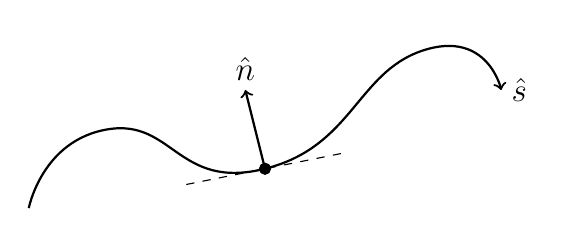
\begin{tikzpicture}
		% Draw the reference path (curved)
		\draw[thick, ->] plot [smooth, tension=1] coordinates {(-3,-1) (-2,0) (0,-0.5) (2,1) (3,0.5)}  node[right] {\large $\hat{s}$};

		% Vehicle position
		\filldraw [black] (0,-0.5) circle (2pt);
		% \node[below left] at (0,-0.5) {\textbf{Vehicle}};

		% Tangent vector (s direction)
		% \draw[->, thick] (0,-0.5) -- (1,0.8);
		% \node[right] at (1,0.8) {\large $\hat{s}$};

		% Normal vector (n direction)
		\draw[->, thick] (0,-0.5) -- (-0.25,0.5);
		\node[above] at (-0.25,0.5) {\large $\hat{n}$};

		% Dashed line for local reference
		\draw[dashed] (-1,-0.7) -- (1,-0.3);
	\end{tikzpicture}
	\caption{Frenet Frame Representation}
	\label{fig:frenet_frame}
\end{figure}

\chapter{Methodology}
\section{Motion Planning Using the Double Integrator Model} \label{sec:motion_planning_using_point_mass}

This section develops a motion planning framework using the double integrator model from \ref{subsec:point_mass_model}, transitioning from a global
coordinate representation to a Frenet frame formulation, as introduced in \ref{subsec:curve_following_coordinate_system}.
The Frenet frame provides a more structured approach for path tracking along a predefined road, accounting for curvature and alignment errors.
Our formulation builds on the work of Eilbrecht et al.
\cite{eilbrecht_challenges_2020} and systematically addresses motion dynamics, constraints, and control strategies.

\subsection{Overview of the Motion Planning Framework}

To effectively model and control vehicle motion, we employ a structured approach that systematically integrates kinematics, dynamics, constraints,
and control transformations.

We begin by defining the \textbf{coordinate transformation and kinematics}, introducing the curvature $C(s)$ of the reference path and the alignment
error $\xi = \psi - \theta$.
These definitions allow us to derive the first- and second-order kinematic equations, which describe how the vehicle's body-fixed velocity components
influence its evolution in Frenet coordinates.

Next, we formulate the \textbf{system dynamics} within the Frenet frame, defining the state vector and control inputs.
By incorporating the effects of curvature and alignment error, we capture both longitudinal and lateral dynamics within our model.

To address the nonlinearities introduced by the curvature terms, we employ \textbf{feedback linearization}.
This process involves assuming alignment to simplify the nonlinear dynamics, enabling the introduction of artificial control variables that linearize
the system.

To ensure that the planned trajectories remain within physical and operational limits, we carefully handle \textbf{constraint formulation}.
We derive bounds on velocity and acceleration and map them from the body-fixed frame to the Frenet frame, thereby enforcing vehicle and road
constraints within the planning model.

A key challenge in motion planning is the presence of \textbf{non-convexities} introduced by curvature-dependent constraints.
To address this, we use \textbf{quantifier elimination} techniques to obtain convex inner approximations of the feasible set.
We explore two approaches:
\begin{itemize}
	\item Interval Fitting, which provides a computationally efficient, box-shaped approximation of the constraint set.
	\item Cylindrical Algebraic Decomposition (CAD), a method from computer algebra that decomposes space into cylindrical cells to eliminate quantifiers while preserving logical equivalence.
\end{itemize}

Once an optimal trajectory is determined, we establish a \textbf{control transformation} that maps the optimized state and control variables to
physical vehicle inputs.
This step derives the necessary steering angle and longitudinal acceleration, ensuring compatibility with standard vehicle controllers.

Next, we provide the \textbf{exact discretization of the double integrator model}, ensuring an accurate transition from continuous to discrete-time
dynamics.
By leveraging matrix exponentials, this formulation preserves system behavior over discrete time steps.

Finally, we present the \textbf{complete motion planning model} as a formalized representation.
This encapsulates the system's state-space dynamics, control inputs, constraints, and transformation mappings.

\subsection{Coordinate Transformation and Kinematics}

In this subsection, we establish the foundation for our motion planning framework by describing the geometry of the reference path and deriving the
vehicle's kinematic equations in the Frenet frame.

First, let \(\theta(s)\) denote the tangent angle at an arc length \(s\) along the reference path.
The curvature, \(C(s)\), quantifies the rate of change of this tangent angle with respect to \(s\) and is defined as:
\begin{equation}
	C(s) := \frac{d\theta}{ds}.
\end{equation}

Next, consider the vehicle's orientation, \(\psi\).
To measure how much the vehicle deviates from following the road's direction, we define the alignment error \(\xi\) as:
\begin{equation}
	\xi := \psi - \theta.
\end{equation}
This error quantifies the difference between the vehicle's heading and the path's tangent direction.

Using these definitions and standard coordinate transformation techniques \cite{eilbrecht_challenges_2020}, we can derive the vehicle's motion
dynamics in the Frenet frame.
In this framework, the velocity components in the vehicle's body-fixed frame are directly related to the time derivatives of the Frenet coordinates.

\paragraph{First-Order Kinematics}\label{par:first_order_kinematics}
The following equations describe how the vehicle's position evolves along the path:
\begin{align}
	\dot{s}\,(1 - n\,C(s)) & = v_x\cos{\xi} - v_y\sin{\xi}, \label{eq:first_derivative_long} \\
	\dot{n}                & = v_x\sin{\xi} + v_y\cos{\xi}, \label{eq:first_derivative_lat}
\end{align}
where:
\begin{itemize}
	\item \(s\) is the longitudinal position along the reference path,
	\item \(n\) represents the lateral deviation from the path,
	\item \(v_x\) and \(v_y\) are the velocity components in the body-fixed frame.
\end{itemize}
Note that the term \(1 - n\,C(s)\) adjusts the longitudinal progress to account for the path's curvature.

\paragraph{Acceleration Dynamics}\label{par:acceleration_dynamics}
To capture the dynamics of acceleration in the Frenet frame, we introduce transformed acceleration components \(a_{x,tn}\) and \(a_{y,tn}\).
These dynamics are given by:
\begin{align}
	a_{x,tn} & = (a_x - v_y\,\dot{\psi})\cos{\xi} - (a_y + v_x\,\dot{\psi})\sin{\xi}, \label{eq:second_derivative_long} \\
	a_{y,tn} & = (a_x - v_y\,\dot{\psi})\sin{\xi} + (a_y + v_x\,\dot{\psi})\cos{\xi}, \label{eq:second_derivative_lat}
\end{align}
with the following definitions:
\begin{align}
	a_{x,tn} & := \ddot{s}\,(1 - n\,C(s)) - 2\dot{n}\,C(s)\dot{s} - n\,C'(s)\dot{s}^2, \label{def:axtn} \\
	a_{y,tn} & := \ddot{n} + C(s)\dot{s}^2\,(1 - n\,C(s)). \label{def:aytn}
\end{align}
These equations illustrate how the vehicle's acceleration in the Frenet frame is influenced by both its inherent dynamics (through \(\ddot{s}\) and
\(\ddot{n}\)) and the geometry of the reference path (through \(C(s)\) and its derivative \(C'(s)\)).

In summary, this subsection defines the key geometric parameters and derives the kinematic equations necessary for representing vehicle motion in the
Frenet frame.
These results set the stage for the subsequent development of the full motion planning model.

\subsection{System Dynamics Formulation}

We can now formalize the motion planning model in the Frenet frame by defining the state and control input vectors.
The state vector, denoted by \(x_{di}\), captures the vehicle's position, alignment error, and their corresponding velocities:
\begin{equation}
	x_{di} = \begin{bmatrix}
		s       \\
		n       \\
		\xi     \\
		\dot{s} \\
		\dot{n} \\
		\dot{\psi}
	\end{bmatrix},
\end{equation}
where:
\begin{itemize}
	\item \(s\) is the longitudinal position along the reference path,
	\item \(n\) is the lateral deviation,
	\item \(\xi\) is the alignment error (\(\psi - \theta\)),
	\item \(\dot{s}\), \(\dot{n}\), and \(\dot{\psi}\) are the corresponding time derivatives.
\end{itemize}

The control inputs are represented by the vector \(u_{di}\), which comprises the body-fixed accelerations:
\begin{equation}
	u_{di} = \begin{bmatrix}
		a_x \\
		a_y \\
		a_\psi
	\end{bmatrix}.
\end{equation}

Using the kinematic relationships derived earlier in \nameref{par:first_order_kinematics} and \nameref{par:acceleration_dynamics}, the dynamics of the double integrator model in the Frenet frame can be expressed as:
\begin{equation}
	\label{eq:frenet_frame_pm_dynamics_0}
	f_{di}(x_{di}, u_{di}) = \begin{bmatrix}
		\dot{s}                                                                                \\
		\dot{n}                                                                                \\
		\dot{\psi} - C(s)\dot{s}                                                               \\
		\displaystyle \frac{a_{x,tn} + 2\dot{n}\,C(s)\dot{s} + n\,C'(s)\dot{s}^2}{1 - n\,C(s)} \\
		a_{y,tn} - C(s)\dot{s}^2(1 - n\,C(s))                                                  \\
		a_\psi
	\end{bmatrix}.
\end{equation}

This formulation captures the vehicle's motion along a curved path by incorporating both its intrinsic dynamics and the influence of road curvature.
It is important to note that the curvature terms \(C(s)\) and \(C'(s)\) introduce non-convexities into the system dynamics.
We address these challenges in subsequent sections through feedback linearization.

\subsection{Linearization via Feedback Control} \label{subsec:constraints}
To simplify the nonlinear dynamics introduced by the curvature terms, we first decouple the body-fixed inputs in
\eqref{eq:frenet_frame_pm_dynamics_0}.
By substituting \eqref{eq:frenet_frame_pm_dynamics_0} the accelerations in the Frenet frame with their body-fixed relations from
\eqref{eq:second_derivative_long} and \eqref{eq:second_derivative_lat} in \eqref{eq:frenet_frame_pm_dynamics_0}, we obtain:
\begin{align}
	\frac{(a_x - v_y\,\dot{\psi})\cos{\xi} - (a_y + v_x\,\dot{\psi})\sin{\xi} + 2\dot{n}\,C(s)\dot{s} + n\,C'(s)\dot{s}^2}{1 - n\,C(s)} \\
	(a_x - v_y\,\dot{\psi})\sin{\xi} + (a_y + v_x\,\dot{\psi})\cos{\xi} - C(s)\dot{s}^2(1 - n\,C(s))
\end{align}
We observe that both entries contain the body-fixed control inputs \(a_x\) and \(a_y\).
To simplify the model, we make the following key assumption.

\subsubsection{Assumption: Alignment Error} \label{subsubsec:alignment_error}
We assume that the vehicle is always aligned with the road, i.e.,
\begin{equation}
	\xi = \psi - \theta = 0.
\end{equation}
This assumption leads to several useful simplifications:
\begin{itemize}
	\item The body-fixed accelerations are directly given by the transformed accelerations:
	      \[
		      [a_x,\, a_y] = [a_{x,tn},\, a_{y,tn}].
	      \]
	\item The rate of change of the vehicle's orientation becomes:
	      \[
		      \dot{\psi} = \dot{\theta} = C(s)\,\dot{s},
	      \]
	      where \(C(s)=\frac{d\theta}{ds}\).
	\item The yaw acceleration satisfies:
	      \[
		      a_\psi = \ddot{\psi} = \ddot{\theta} = C'(s)\,\dot{s}^2 + C(s)\,\ddot{s}.
	      \]
\end{itemize}
Although this assumption fixes the orientation to the road, the vehicle is still permitted lateral movement via lateral acceleration.

With this alignment assumption, the dynamics become affine in \(a_{x,tn}\) and \(a_{y,tn}\).
This property allows us to introduce artificial control inputs that will fully linearize the system.

\subsubsection{Introducing Artificial Control Inputs}

Define the artificial control input vector \(\tilde{u}_{di}\) as:
\begin{equation}
	\label{eq:artificial_controls}
	\tilde{u}_{di} := \begin{bmatrix}
		u_t \\
		u_n
	\end{bmatrix} :=
	\begin{bmatrix}
		\displaystyle \frac{a_{x,tn} + 2\dot{n}\,C(s)\dot{s} + n\,C'(s)\dot{s}^2}{1 - n\,C(s)} \\
		a_{y,tn} - C(s)\dot{s}^2(1 - n\,C(s))
	\end{bmatrix}.
\end{equation}
These artificial control inputs will be used to linearize the system dynamics, a process known as feedback linearization.
This technique is thoroughly explained in \cite{khalil_nonlinear_2002}.
In the following section, we will briefly introduce the concept of feedback linearization before applying it in our motion planning framework.

\subsubsection{Supplementary Background: Feedback Linearization}

Feedback linearization is a nonlinear control technique that transforms a nonlinear system into an equivalent linear system by means of a suitable
change of variables and state-feedback law.
Consider a general nonlinear system of the form:
\begin{equation}
	\dot{x} = f(x) + G(x)\,u,
\end{equation}
where
\begin{itemize}
	\item \(x \in \mathbb{R}^n\) is the state vector,
	\item \(f(x)\) represents the system dynamics,
	\item \(G(x)\) is the input matrix,
	\item \(u \in \mathbb{R}^m\) is the control input.
\end{itemize}
For feedback linearization, it is typical to assume that the system is fully actuated, i.e., \[ \text{rank}\bigl(G(x)\bigr) = n, \] ensuring that
\(G(x)\) is invertible in the region of interest.
Under this assumption, one can define a new control input \(v\) such that:
\begin{equation}
	u = G(x)^{-1}\,\bigl[v - f(x)\bigr].
\end{equation}
By canceling the nonlinear dynamics \(f(x)\), the new input \(v\) governs an equivalent linear system that can be addressed with standard linear
control techniques.

\subsubsection{Resulting Simplified Model}\label{subsubsec:resulting_simplified_model}

Returning to our model, we can use the artificial control inputs \(\tilde{u}_{di}\) to linearize the system dynamics.
Given our assumption of no alignment error \ref{subsubsec:alignment_error}, the state variables can be simplified by removing the orientation
\(\psi\), as it is fixed to the road.
The reduced state vector is:
\[
	\tilde{x}_{di} = \begin{bmatrix} s, & n, & \dot{s}, & \dot{n} \end{bmatrix}^T,
\]
and the new artificial control inputs are:
\[
	\tilde{u}_{di} = \begin{bmatrix} u_t, & u_n \end{bmatrix}^T.
\]
Under these definitions, the system dynamics simplify to:
\begin{equation}
	\label{eq:pm_final_dynamics}
	\tilde{f}_{di}(\tilde{x}_{di}, \tilde{u}_{di}) = \begin{bmatrix}
		\dot{s} \\
		\dot{n} \\
		u_t     \\
		u_n
	\end{bmatrix}.
\end{equation}

With the dynamics now expressed in a simplified, linear form, our next task is to ensure that the planned trajectories adhere to both the vehicle's
physical limitations and the geometric constraints of the road.
In the following section, we establish the coupling constraints between the state variables and control inputs for our discrete-time optimal
trajectory planning problem (see \eqref{eq:coupling_constraints}) based on \cite{eilbrecht_challenges_2020}.

\subsection{Constraint Handling}

This subsection addresses the constraints imposed by the vehicle's physical limits and the road geometry.
We first define the constraints on state variables and control inputs in the body-fixed frame and then map them to the Frenet frame.
This mapping allows us to formulate the overall coupling constraint set that must be satisfied during trajectory planning.
We will also discuss the challenge of non-convexity arising from these coupling constraints and formulate the problem of finding a convex
under-approximation.

Let \(\square\) denote any planning variable.
For each variable, we define constant upper and lower bounds during planning, denoted by \(\overline{\square}\) and \(\underline{\square}\),
respectively.
For example, in the vehicle's body-fixed frame the velocity constraints are expressed as:
\begin{align}
	\underline{v_x} \leq v_x \leq \overline{v_x}, \\
	\underline{v_y} \leq v_y \leq \overline{v_y}.
\end{align}

By applying the first-order kinematics from \eqref{eq:first_derivative_long} and \eqref{eq:first_derivative_lat} with the alignment error set to \(\xi=0\), these velocity bounds translate into the Frenet frame as follows:
\begin{align}
	\underline{v_x} \leq \dot{s}\,(1 - n\,C(s)) \leq \overline{v_x}, \\
	\underline{v_y} \leq \dot{n} \leq \overline{v_y}.
\end{align}
Here, \(\dot{s}\) represents the longitudinal speed adjusted by the term \((1 - n\,C(s))\) to account for the curvature of the road, and \(\dot{n}\)
is the lateral speed.

For acceleration constraints, we typically define two types:
\begin{itemize}
	\item A norm constraint that limits the overall acceleration, ensuring that the combined longitudinal and lateral accelerations lie within a circle of radius \(c\), similar to \eqref{eq:acceleration_constraint_preliminaries_di}:
	      \begin{equation}
		      a_x^2 + a_y^2 \leq c.
	      \end{equation}
	\item Individual bounds on the longitudinal and lateral accelerations:
	      \begin{align}
		      \underline{a_x} \leq a_x \leq \overline{a_x}, \\
		      \underline{a_y} \leq a_y \leq \overline{a_y}.
	      \end{align}
\end{itemize}

To map these acceleration constraints to the Frenet frame, we use the definition \eqref{eq:artificial_controls} of our artificial variables
\eqref{eq:artificial_controls} and the first implication $a_x=a_{x,tn}$ and $a_y=a_{y,tn}$ from our alignment error assumption
\ref{subsubsec:alignment_error}.
These equations allow us to establish a mapping that relates the state variables and artificial control inputs \((\tilde{x}_{di}, \tilde{u}_{di})\)
to the body-fixed accelerations by solving for $a_x$ and $a_y$.
This mapping is defined as:
\begin{equation}
	\label{def:g}
	g(\tilde{x}_{di}, \tilde{u}_{di}) :=
	\begin{bmatrix}
		(1 - n\,C(s))\,u_t - \bigl(2\dot{n}\,C(s)\dot{s} + n\,C'(s)\dot{s}^2\bigr) \\
		u_n + C(s)\,\dot{s}^2\,(1 - n\,C(s))
	\end{bmatrix}
	=
	\begin{bmatrix}
		a_x \\
		a_y
	\end{bmatrix}.
\end{equation}
Substituting this mapping into the individual acceleration constraints, we derive the following bounds in the Frenet frame:
\begin{align}
	\begin{bmatrix}
		\underline{a_x} \\[2mm] \underline{a_y}
	\end{bmatrix} \leq g(\tilde{x}_{di}, \tilde{u}_{di}) \leq \begin{bmatrix}
		                                                          \overline{a_x} \\[2mm] \overline{a_y}
	                                                          \end{bmatrix} \\[2mm]
	\|g(\tilde{x}_{di}, \tilde{u}_{di})\|^2 \leq c.
\end{align}

Next, we need to impose limits on the yaw rate and yaw acceleration.
The yaw rate is defined as \(C(s)\,\dot{s}\), and the yaw acceleration is given by \(C'(s)\,\dot{s}^2 + C(s)\,u_t\), as derived from the second and
third implications of our alignment error assumption \ref{subsubsec:alignment_error}.
\begin{align}
	\underline{\dot{\psi}} \leq C(s)\,\dot{s} \leq \overline{\dot{\psi}}, \\
	\underline{a_{\psi}} \leq C'(s)\,\dot{s}^2 + C(s)\,u_t \leq \overline{a_{\psi}}.
\end{align}

Thus, we have successfully modeled the physical limits of the vehicle in the Frenet frame.
The constraints arising from the road topology can be represented using the Frenet frame coordinates from our state variables, \(s\) and \(n\).
To adhere to DCP rules, we allow the lateral range to depend on the arc length \(s\).
This is achieved by defining the bounds \(\underline{n}(s)\) and \(\overline{n}(s)\) for the lateral deviation, where \(\underline{n}(s)\) is convex
in \(s\) and \(\overline{n}(s)\) is concave in \(s\).
The arc length \(s\) is constrained by the constant bounds \(\underline{s}\) and \(\overline{s}\).

Combining all introduced constants, the overall coupling constraint set \(\mathcal{C}\) is defined as:
\begin{equation}
	\mathcal{C} := \left\{
	\begin{bmatrix} \tilde{x}_{di} \\ \tilde{u}_{di} \end{bmatrix} \; \middle|\;
	\begin{aligned}
		 & \underline{s} \leq s \leq \overline{s},                                                        \\
		 & \underline{n}(s) \leq n \leq \overline{n}(s),                                                  \\
		 & \underline{v_x} \leq \dot{s}\,(1 - n\,C(s)) \leq \overline{v_x},                               \\
		 & \underline{v_y} \leq \dot{n} \leq \overline{v_y},                                              \\
		 & \underline{\dot{\psi}} \leq C(s)\,\dot{s} \leq \overline{\dot{\psi}},                          \\
		 & \underline{a_{\psi}} \leq C'(s)\,\dot{s}^2 + C(s)\,u_t \leq \overline{a_{\psi}},               \\
		 & \begin{bmatrix}
			   \underline{a_x} \\[2mm] \underline{a_y}
		   \end{bmatrix} \leq g(\tilde{x}_{di}, \tilde{u}_{di}) \leq \begin{bmatrix}
			                                                             \overline{a_x} \\[2mm] \overline{a_y}
		                                                             \end{bmatrix}, \\
		 & \|g(\tilde{x}_{di}, \tilde{u}_{di})\|^2 \leq c.
	\end{aligned}
	\right\}.
\end{equation}

The constraint set \(\mathcal{C}\) is highly non-convex, primarily due to the curvature terms \(C(s)\) and \(C'(s)\) and their nonlinear interaction
with the state and control inputs.
To handle this non-convexity, we seek to derive a convex inner approximation of the feasible set \(\mathcal{C}\).
This objective is defined here and addressed in the following section.

\subsubsection{Problem Definition: Finding an Inscribed Polytope}
\label{problem:inscribed_polytope}

To handle the non-convexity, our approach is to approximate \(\mathcal{C}\) with an inscribed polytope \(\hat{C}\) that is convex.
Formally, we seek to determine:
\begin{equation}
	\hat{C} = \left\{ \begin{bmatrix}
		\tilde{x}_{di} \\[2mm] \tilde{u}_{di}
	\end{bmatrix} \; \middle|\;
	N \begin{bmatrix}
		\tilde{x}_{di} \\[2mm] \tilde{u}_{di}
	\end{bmatrix} \leq b
	\right\} \subseteq \mathcal{C},
\end{equation}
where \(N\) and \(b\) represent a set of linear inequalities whose intersection forms the polytope.
In the following section, we will demonstrate how to address this problem.

\subsection{Convex Approximation via Quantifier Elimination}
This section addresses the problem of determining an inscribed polytope, as defined in Problem \ref{problem:inscribed_polytope}.
Our approach begins by simplifying the original constraint set through dimensionality reduction.

To achieve this, we decouple the state variables $s$, $n$, and $\dot{n}$, each of which is independently constrained within an interval:

\begin{align}
	\label{eq:state_constraints}
	\underline{s} \leq s \leq \overline{s},       \\
	\underline{n}(s) \leq n \leq \overline{n}(s), \\
	\underline{\dot{n}} \leq \dot{n} \leq \overline{\dot{n}}.
\end{align}

By ensuring that the remaining constraints hold for all values of $s$, $n$, and $\dot{n}$ within their respective intervals, we effectively reduce
the problem to a lower-dimensional space involving only the remaining variables.

We define the reduced constraint set, $\tilde{C}$, over the variables $\dot{s}$ and the artificial control inputs $\tilde{u}_{di}$ as follows:

\begin{equation}
	\tilde{C} =
	\left\{ \;
	\begin{bmatrix}
		\dot{s} \\
		u_t     \\
		u_n
	\end{bmatrix}
	\; \middle|\;
	\begin{bmatrix}
		\tilde{x}_{di} \\ \tilde{u}_{di}
	\end{bmatrix} \in \mathcal{C}, \quad \forall
	\begin{bmatrix}
		s \\
		n \\
		\dot{n}
	\end{bmatrix} \in
	\begin{bmatrix}
		\underline{s}, \overline{s} \\
		\underline{n}, \overline{n} \\
		\underline{\dot{n}}, \overline{\dot{n}}
	\end{bmatrix}
	\right\}.
\end{equation}

To make $\tilde{C}$ practically useful, we aim to express it as a set of linear inequalities.
Since quantifiers cannot be directly modeled according to the DCP rules, we need to eliminate them.

The task of expressing $\tilde{C}$ as linear inequalities can be framed as a problem of \textbf{quantifier elimination}, a common technique in
computer algebra.
The goal of quantifier elimination is to transform a formula containing quantified variables into an equivalent form without quantifiers.

In our case, the constraint set can be expressed as the quantified formula:

\begin{equation}
	\label{eq:forall_formula}
	\phi :=
	\forall
	\begin{bmatrix}
		s \\
		n \\
		\dot{n}
	\end{bmatrix} \in
	\begin{bmatrix}
		\underline{s}, \overline{s} \\
		\underline{n}, \overline{n} \\
		\underline{\dot{n}}, \overline{\dot{n}}
	\end{bmatrix}: \quad
	\begin{aligned}
		 & \underline{v_x} \leq \dot{s}(1-nC(s)) \leq \overline{v_x} \quad \land                         \\
		 & \underline{\dot{\psi}} \leq C(s)\dot{s} \leq \overline{\dot{\psi}} \quad \land                \\
		 & \underline{a_{\psi}} \leq C'(s)\dot{s}^2 + C(s)u_t \leq \overline{a_{\psi}} \quad \land       \\
		 & \begin{bmatrix}
			   \underline{a_x} \\[2mm] \underline{a_y}
		   \end{bmatrix} \leq g(\tilde{x}_{di},\tilde{u}_{di}) \leq \begin{bmatrix}
			                                                            \overline{a_x} \\[2mm] \overline{a_y}
		                                                            \end{bmatrix} \quad \land \\
		 & \|g(\tilde{x}_{di}, \tilde{u}_{di})\|^2 \leq c.
	\end{aligned}
\end{equation}

Typically, quantifier elimination seeks a formula $\phi'$ such that:

\[ \phi' \iff \phi \] where $\phi'$ contains no quantifiers.
However, in our case, we relax this requirement and allow $\phi'$ to be a sufficient condition for $\phi$, meaning:

\[ \phi'
	\implies \phi \]

This means that $\phi'$ describes a subset of $\tilde{C}$.
This relaxation has two advantages:

It enables more efficient algorithms for quantifier elimination, as we do not need an exact
equivalent formula, and it may be necessary, as $\tilde{C}$ is not guaranteed to be convex.

We propose two approaches to eliminate the quantifiers in $\phi$ and express $\tilde{C}$ as a set of linear inequalities.
The first approach involves interval fitting for the state variables and control inputs, and we will present the results to facilitate replication.
The second approach uses Cylindrical Algebraic Decomposition (CAD) to eliminate the quantifiers.
Since CAD has multiple implementations and explaining this complex algorithm is beyond the scope of this work, we will only present the idea behind
it by demonstrating the algorithm on an example.
Finally, we will compare the results of both approaches and discuss their advantages and disadvantages.

Either approach will provide us with a polytope $\tilde{C}$, which we can use to define the solution to Problem:
\begin{equation}
	\label{eq:pm_coupling_constraints}
	\hat{C} = \tilde{C} \times [\underline{s}, \overline{s}] \times [\underline{n}, \overline{n}] \times [\underline{\dot{n}}, \overline{\dot{n}}]
\end{equation}

\subsubsection{Approach 1: Interval Fitting for State Variables and Control Inputs} \label{subsubsec:interval_fitting}
The idea of the first approach is to find intervals for the variables of interest, namely $\dot{s}$, $u_t$, and $u_n$, such that for any values these
variables may take within those intervals, the implications from \eqref{eq:forall_formula} hold.
Each condition of these implications follows a specific pattern.
Let $x \in \{\dot{s}, u_t, u_n\}$ and $y$ be a vector containing the remaining variables that are part of the condition.
\begin{equation}
	\label{eq:cur_condition}
	c_{min} \leq f(x, y) \leq c_{max}
\end{equation}
where $x \in \mathbb{R}$, $y \in \mathbb{R}^n$, and $f: \mathbb{R}^{n+1} \to \mathbb{R}$, with constants $c_{min}, c_{max} \in \mathbb{R}$.
The variable $x$ is selected such that all other variables contained in $y$ are bounded.
Additionally, $x$ is chosen so that $f$ is affine in $x$, represented by:
\begin{equation}
	f(x, y) = a(y) x + b(y)
\end{equation}
where $a, b : \mathbb{R}^n \to \mathbb{R}$. Since $a$ and $b$ are continuous functions over a bounded domain $Y$, we can find bounds on $a(y)$ and $b(y)$:
\begin{equation}
	a_{min} \leq a(y) \leq a_{max}, \quad b_{min} \leq b(y) \leq b_{max}
\end{equation}
Our goal is to find an interval $[\underline{x}, \overline{x}]$ for $x$ such that
\begin{equation}
	x\in [\underline{x}, \overline{x}] \implies \forall y\in Y: c_{min} \leq f(x, y) \leq c_{max}
\end{equation}

We define $X := [\underline{x}, \overline{x}]$.
To calculate $X$, we perform a case distinction based on the possible signs of $a(y)$.
Let's start with

\textbf{1.
}
$a(y) > 0$:
We can subtract \eqref{eq:cur_condition} with $b(y)$ and divide by $a(y)$:
\[
	\frac{c_{min}-b(y)}{a(y)} \leq x \leq \frac{c_{max}-b(y)}{a(y)}
\]
Since we have to ensure the condition holds even in the worst case, $X$ is given by:
\[
	\underline{x} =
	\begin{cases}
		\begin{array}{ll}
			\frac{c_{min}-b_{min}}{a_{max}}, & \text{if } c_{min}-b_{min} < 0 \\[10pt]
			\frac{c_{min}-b_{min}}{a_{min}}, & \text{otherwise}
		\end{array}
	\end{cases}
\]
\[
	\overline{x} =
	\begin{cases}
		\begin{array}{ll}
			\frac{c_{max}-b_{max}}{a_{min}}, & \text{if } c_{max}-b_{max} < 0 \\[10pt]
			\frac{c_{max}-b_{max}}{a_{max}}, & \text{otherwise}
		\end{array}
	\end{cases}
\]

\textbf{2.}
$a(y) \geq 0$:
Since $a(y) = 0$ for some $y\in Y$, we have to test if this condition holds:
\[
	c_{min} \leq b_{min} \text{ and } b_{max} \leq c_{max}
\]
If this condition does not hold, then $X=\emptyset$.
Otherwise, we exclude all $y \in Y$ for which $a(y)=0$ and proceed to the first case.

\textbf{3.}
$a(y) < 0$:
We can again subtract $b(y)$ from \eqref{eq:cur_condition} and divide by $a(y)$, but this time the direction of the inequalities changes:
\[
	\frac{c_{max}-b(y)}{a(y)} \leq x \leq \frac{c_{min}-b(y)}{a(y)}
\]
and by looking at the worst cases of the lower and upper bound, we can calculate $X$:
\[
	\underline{x} =
	\begin{cases}
		\begin{array}{ll}
			\frac{c_{max}-b_{max}}{a_{max}}, & \text{if } c_{max}-b_{max} < 0 \\[10pt]
			\frac{c_{max}-b_{max}}{a_{min}}, & \text{otherwise}
		\end{array}
	\end{cases}
\]
\[
	\overline{x} =
	\begin{cases}
		\begin{array}{ll}
			\frac{c_{min}-b_{min}}{a_{min}}, & \text{if } c_{min}-b_{min} < 0 \\[10pt]
			\frac{c_{min}-b_{min}}{a_{max}}, & \text{otherwise}
		\end{array}
	\end{cases}
\]

\textbf{4.}
$a(y) \leq 0$:
Similar to the second case, we need to check if $c_{min} \leq b_{min}$ and $b_{max} \leq c_{max}$ hold.
If not, set $X=\emptyset$.
Otherwise, ignore the values where $a(y)$ equals zero and proceed to the third case.

\textbf{5.}
We have so far considered all the cases where $a(y)$ cannot take both positive and negative values.
We now consider the last case, where $a_{min} < 0$ and $a_{max} > 0$.
Since $a(y) = 0$ for some values, we first check if $c_{min} \leq b_{min}$ and $b_{max} \leq c_{max}$.
If this condition does not hold, we set $X = \emptyset$.
Otherwise, $X$ is given by:

\[ \underline{x} = \max \left\{ \frac{c_{min} - b_{min}}{a_{max}}, \frac{c_{max} - b_{max}}{a_{min}}
	\right\} \]

\[ \overline{x} = \min \left\{ \frac{c_{max} - b_{max}}{a_{max}}, \frac{c_{min} - b_{min}}{a_{min}} \right\} \]

If we end up with $x_{max} < x_{min}$, set $X=\emptyset$.

All of this applies nicely to our scenario, as we can systematically apply these rules to each constraint step by step.
The resulting polytope, based on the interval approach, is box-shaped.
This shape further reduces our set of possible state variables and control inputs.

\subsubsection{Approach 2: Cylindrical Algebraic Decomposition} \label{subsubsec:cad}

The second approach is to use Cylindrical Algebraic Decomposition (CAD) to find the inscribed polytope.
This method is computationally more expensive but provides a more accurate result.
The idea is to find an equivalent formula without quantifiers for a given formula containing quantifiers.
This can be done using CAD.

CAD is a method used in computer algebra for solving systems of polynomial equations and inequalities.
Given a set of polynomial equations and inequalities, CAD decomposes the space into a finite number of cylindrical cells.
Each cell is described by a sequence of polynomial inequalities and has a constant truth value over the input set of polynomial equations and
inequalities.
This way, one only needs to pick one point from each cell to check the truth value of the input set.
The number of cells grows doubly exponentially with the number of variables in the input set.
Several implementations of CAD exist.

We will illustrate how the algorithm works, but it is beyond the scope of this work to explain the implementations in detail.
Instead, we provide a basic example to illustrate the algorithm without delving into the details.
You can find more information in the literature \cite{caviness_quantifier_1998, england_cylindrical_2020}.

\subsubsection{Example CAD}
To illustrate the process of eliminating $\forall$ quantifiers, consider the following problem:

\[ \forall x, x^2 + bx + 1 \geq 0
\]

Since quantifier elimination is typically performed on existential quantifiers, we first solve the problem for:

\[ \exists x, x^2 + bx + 1 < 0 \]

Once we have the solution for this problem, we can take the compliment over
$\mathbb{R}$ to obtain the solution for the original problem.
We start by applying CAD to the polynomial $x^2 + bx + 1$, which results in 7 cells, as illustrated in Figure \ref{fig:example_cells}.
Most of the cells are open, and if the edge of the cell is part of it, it is depicted with the same color but dashed.

\begin{figure}[h]
	\centering
	\definecolor{redviolet}{rgb}{0.78, 0.08, 0.52}
	\begin{tikzpicture}
		\begin{axis}[
				xlabel={$b$},
				ylabel={$x$},
				axis lines=middle,
				enlargelimits=true,
				legend pos=north west,
			]

			% Define the boundaries as paths
			\addplot [name path=RightUpper, domain=2:5, samples=100, thick, redviolet!30, dashed] {-(x/2) + 1/2 * sqrt(-4 + x^2)};
			\addplot [name path=RightLower, domain=2:5, samples=100, thick, teal!30, dashed] {-(x/2) - 1/2 * sqrt(-4 + x^2)};
			\addplot [name path=LeftUpper, domain=-5:-2, samples=100, thick,blue!30, dashed] {-(x/2) + 1/2 * sqrt(-4 + x^2)};
			\addplot [name path=LeftLower, domain=-5:-2, samples=100, thick,cyan!30, dashed] {-(x/2) - 1/2 * sqrt(-4 + x^2)};

			% Define vertical lines as paths but make them invisible
			\addplot [name path=lineInnerRight,dashed, thick,  red!30] coordinates {(2,-5) (2,5)};
			\addplot [name path=lineInnerLeft, dashed, thick, red!30] coordinates {(-2,-5) (-2,5)};

			% Define horizontal boundaries as paths but make them invisible
			\addplot [name path=lineUpperLeft, draw=none] coordinates {(-5,5) (-2,5)};
			\addplot [name path=lineUpperRight, draw=none] coordinates {(2,5) (5,5)};
			\addplot [name path=lineLowerLeft, draw=none] coordinates {(-5,-5) (-2,-5)};
			\addplot [name path=lineLowerRight, draw=none] coordinates {(2,-5) (5,-5)};

			% Region 1: b>2, x >= -(b/2) + 1/2 sqrt(-4 + b^2)
			\addplot [fill=redviolet!30, opacity=0.5] fill between[of=RightUpper and lineUpperRight];

			% % Region 2: b>2, x <= -(b/2) - 1/2 sqrt(-4 + b^2)
			\addplot [fill=teal!30, opacity=0.5] fill between[of=RightLower and lineLowerRight];

			% % Region 3: b<-2, x >= -(b/2) + 1/2 sqrt(-4 + b^2)
			\addplot [fill=blue!30, opacity=0.5] fill between[of=LeftUpper and lineUpperLeft];

			% % Region 4: b<-2, x <= -(b/2) - 1/2 sqrt(-4 + b^2)
			\addplot [fill=cyan!30, opacity=0.5] fill between[of=LeftLower and lineLowerLeft];

			% % Region 5: -2 ≤ b ≤ 2 (rectangle covering all x values)
			\addplot [fill=red!30, opacity=0.5] fill between[of=lineInnerLeft and lineInnerRight];

			% % Region 6: b>2, x > -(b/2) - 1/2 Sqrt[-4+b^2], x < -(b/2) + 1/2 Sqrt[-4+b^2]
			\addplot [fill=cyan!30, opacity=0.3] fill between[of=RightUpper and RightLower];

			% % Region 7: b<-2, x > -(b/2) - 1/2 Sqrt[-4+b^2], x < -(b/2) + 1/2 Sqrt[-4+b^2]
			\addplot [fill=gray!30, opacity=0.3] fill between[of=LeftUpper and LeftLower];

		\end{axis}
	\end{tikzpicture}
	\caption{Illustrating the cells with shaded regions.}
	\label{fig:example_cells}
\end{figure}
We now need to check the truth value of the polynomial inequality $x^2 + bx + 1 < 0$ for each cell by picking a random sample and evaluating the
inequality.
The cells where the inequality holds true are colored in green and then projected onto the $b$-axis.
The resulting intervals are the solution to the existential quantifier elimination, which is $(-\infty, -2) \cup (2, \infty)$.
As an input to the algorithm, one must define an order of precedence for the variables.
In its first phase, the algorithm projects the space iteratively from $\mathbb{R}^n$ to $\mathbb{R}^{n-1}$ until it reaches $\mathbb{R}^1$.
This is done by removing one of the remaining variables in each iteration, starting with the last in the order of precedence.
Therefore, if $b$ is defined as the first variable, the sets of polynomial inequalities for each cell will always contain an interval for $b$, which
corresponds to the projection on the axis.
This allows us to directly read the resulting intervals, which is shown in Figure \ref{fig:remaining_cells}.

\begin{figure}[h]
	\centering
	\begin{tikzpicture}
		\begin{axis}[
				xlabel={$b$},
				ylabel={$x$},
				axis lines=middle,
				enlargelimits=true,
				legend pos=north west,
			]

			% Define the boundaries as paths
			\addplot [name path=RightUpper, domain=2:5, samples=100, thick, black!30, dashed] {-(x/2) + 1/2 * sqrt(-4 + x^2)};
			\addplot [name path=RightLower, domain=2:5, samples=100, thick, black!30, dashed] {-(x/2) - 1/2 * sqrt(-4 + x^2)};
			\addplot [name path=LeftUpper, domain=-5:-2, samples=100, thick,black!30, dashed] {-(x/2) + 1/2 * sqrt(-4 + x^2)};
			\addplot [name path=LeftLower, domain=-5:-2, samples=100, thick,black!30, dashed] {-(x/2) - 1/2 * sqrt(-4 + x^2)};

			% Define vertical lines as paths but make them invisible
			\addplot [name path=lineInnerRight,dashed, thick,  draw=none] coordinates {(2,-5) (2,5)};
			\addplot [name path=lineInnerLeft, dashed, thick, draw=none] coordinates {(-2,-5) (-2,5)};

			% Define horizontal boundaries as paths but make them invisible
			\addplot [name path=lineUpperLeft, draw=none] coordinates {(-5,5) (-2,5)};
			\addplot [name path=lineUpperRight, draw=none] coordinates {(2,5) (5,5)};
			\addplot [name path=lineLowerLeft, draw=none] coordinates {(-5,-5) (-2,-5)};
			\addplot [name path=lineLowerRight, draw=none] coordinates {(2,-5) (5,-5)};

			% % Region 6: b>2, x > -(b/2) - 1/2 Sqrt[-4+b^2], x < -(b/2) + 1/2 Sqrt[-4+b^2]
			\addplot [fill=green!30, opacity=0.3] fill between[of=RightUpper and RightLower];

			% % Region 7: b<-2, x > -(b/2) - 1/2 Sqrt[-4+b^2], x < -(b/2) + 1/2 Sqrt[-4+b^2]
			\addplot [fill=green!30, opacity=0.3] fill between[of=LeftUpper and LeftLower];

			\node[circle,draw,inner sep=1pt, green!60] (openCircleRight) at (axis cs:2,0) {};
			\draw[thick, green!60] (openCircleRight) -- (axis cs:5.5,0);
			\node[circle,draw,inner sep=1pt, green!60] (openCircleLeft) at (axis cs:-2,0) {};
			\draw[thick, green!60] (openCircleLeft) -- (axis cs:-5.5,0);
		\end{axis}
	\end{tikzpicture}
	\caption{Illustrating the remaining cells.}
	\label{fig:remaining_cells}
\end{figure}
Since $(-\infty, -2) \cup (2, \infty)$ is the solution for $\exists x, x^2 + bx + 1 < 0$, the solution for the original problem is obtained by taking
the complement of this set:

\[ \forall x, x^2 + bx + 1 \geq 0 \iff b \in [-2, 2] \]

Using this technique for
eliminating quantifiers from formulas, we can apply it to find an inscribed polytope.

\subsubsection{Comparison of Interval Fitting and CAD Approaches}

In our benchmarks, the first approach, despite its simplicity, performed remarkably well.
We used the following parameters for the benchmarks:
\begin{itemize}
	\item $C(s) \in \left[-\frac{1}{200}, 0\right]$, $s \in [0, 10]$, $n \in [0, 2]$
	\item $v_x \in [0, 10]$, $v_y \in [-2, 2]$, $a_x \in [-3, 6]$, $a_y \in [-4, 4]$
	\item $\dot{\psi} \in [-5, 5]$, $a_\psi \in [-2, 2]$
\end{itemize}

The results are shown in the following Figure \ref{fig:qe-comparison}.

\begin{figure}[h]
	\centering
	% First image
	\begin{subfigure}[b]{0.32\textwidth}
		\centering
		\includegraphics[width=\textwidth]{figures/inner_polytope/region_x3u1_plot_gr1.eps}
		\caption{Region $\dot{s}$ vs $u_t$}
	\end{subfigure}
	% Second image
	\begin{subfigure}[b]{0.32\textwidth}
		\centering
		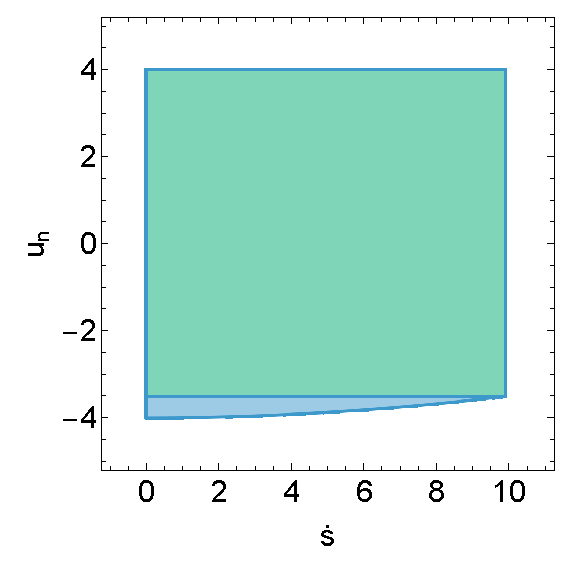
\includegraphics[width=\textwidth]{figures/inner_polytope/region_x3u2_plot_gr1.eps}
		\caption{Region $\dot{s}$ vs $u_n$}
	\end{subfigure}
	% Third image
	\begin{subfigure}[b]{0.32\textwidth}
		\centering
		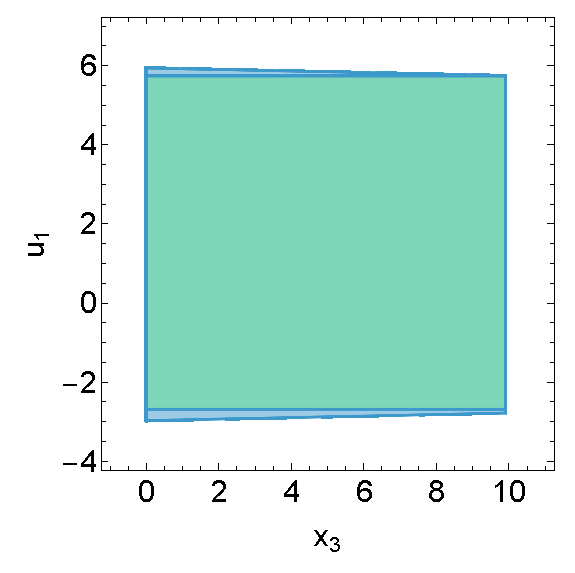
\includegraphics[width=\textwidth]{figures/inner_polytope/plot_gr1.eps}
		\caption{Region $u_t$ vs $u_n$}
	\end{subfigure}
	\caption{In Green using Interval Fitting \ref{subsubsec:interval_fitting} and in Blue using CAD \ref{subsubsec:cad}.}
	\label{fig:qe-comparison}
\end{figure}

In conclusion, eliminating the quantifiers with the first approach leads to a near-optimal result, comparable to the one achieved using the second
approach with CAD.
However, using CAD has a significant downside that we have not yet mentioned.
It is not guaranteed that the resulting formula is convex.
Typically, you will encounter disjunctions of polynomial inequalities, which cannot be handled by a convex solver without resorting to integer
programming or an equivalent approach.
It is also not guaranteed that each polynomial inequality follows the DCP rules, even if the set described by the resulting formula is convex.
Additional techniques would be required to use the second approach for our planner.

In cases where the resulting set is convex, we used a sampling approach to obtain an inner approximation described by half-spaces.
This results in a sequence of linear constraints that all must be satisfied, thus losing a small proportion of the original set.
Consequently, the difference between our first approach and the second approach becomes even smaller.
Additionally, we end up with double or triple the number of constraints on each state variable and each control input, which may lead to slower
solver times.

Overall, while the CAD approach provides a more accurate result, the first approach offers a good balance between computational efficiency and
accuracy, making it a viable option for practical applications.

\subsubsection{Limitations and Outlook}\label{subsubsec:limitations_and_outlook}

While the $\forall$-elimination approach provides a computationally efficient method to find intervals for the variables of interest, it can be quite restrictive for several reasons:

\begin{itemize}
	\item \textbf{Conservativeness:}
	      The approach tends to be conservative because it ensures that the constraints hold for all possible values within the intervals.
	      This often leads to smaller intervals, which may exclude feasible solutions that could be considered by less conservative methods.
	\item \textbf{Dependence on Affine Functions:}
	      The first method relies on the assumption that the function $f(x, y)$ is affine in $x$ and all variables in $y$ are bounded.
	      If this assumption does not hold, the approach may not be applicable.
\end{itemize}

Overall, while the $\forall$-elimination approach is useful for its simplicity and computational efficiency, it may lead to overly restrictive
solutions that do not fully exploit the feasible region.

Consider a scenario with a tight turn followed by a long straight road.
In such cases, the model will restrict $\dot{s}$ to an interval that is valid for both the tight turn and the straight road.
Consequently, the model will find a solution, but it will not be able to drive fast on the straight road, even though it is possible to drive faster
on the straight road than on the tight turn.

To address this issue, we can introduce segments of the road, one for the straight road and one for the tight turn.
We can independently construct the coupling constraints set for each segment.
However, this introduces a new problem: how to switch between the segments.
Our solution involves using the current vehicle velocity to predict when the vehicle will reach the end of the segment.
Knowing the vehicle's current position, velocity, and the distance to the end of the segment, we can calculate the time it will take to reach the
end.

Further, both approaches do not consider the possibility of achieving a larger feasible set by restricting $\dot{n}$ to a smaller interval.
The first approach handles the problem by using the bounds on $s$, $n$, and $\dot{n}$ to find the intervals for $\dot{s}$, which are then used for
$u_t$ and finally for $u_n$.
However, changing the order may lead to better results for desired driving behavior.

Given the simplicity of the first approach, we implemented a non-linear program that defines the relationships between the intervals with variables
as upper and lower bounds.
By adding constraints, we can define an objective that models certain driving behaviors.
For example, one might want to be able to slow down as quickly as possible or maximize the upper speed limit.
The latter objective leads to the following intervals:

\begin{figure}[h]
	\centering
	\begin{subfigure}[b]{0.45\textwidth}
		\centering
		\begin{align*}
			0    & \leq s \leq 10       \\
			0    & \leq n \leq 2        \\
			0    & \leq \dot{s} \leq 10 \\
			-2   & \leq \dot{n} \leq 2  \\
			-2.9 & \leq u_t \leq 5.9    \\
			-4   & \leq u_n \leq 3.75
		\end{align*}
		\caption{Initial Approach}
	\end{subfigure}
	\hfill
	\begin{subfigure}[b]{0.45\textwidth}
		\centering
		\begin{align*}
			0      & \leq s \leq 10,         \\
			0      & \leq n \leq 2,          \\
			0      & \leq \dot{s} \leq 10.05 \\
			-2     & \leq \dot{n} \leq 2     \\
			-2.899 & \leq u_t \leq 5.929     \\
			-4     & \leq u_n \leq 3.746
		\end{align*}
		\caption{Using Non-Linear Programming}
	\end{subfigure}
	\caption{Comparison of two sets of intervals for state variables and control inputs.}
\end{figure}

As you can see, the intervals on the right are preferable, as they only slightly reduce longitudinal acceleration while allowing for higher speeds.

In conclusion, we have successfully developed our first vehicle model for motion planning that can be solved using a convex solver.
Next, we will introduce a transformation that maps the state variables and control inputs of the planning model to a steering angle, which can be
used to control a vehicle based on the equations from \cite{eilbrecht_challenges_2020}.
A similar approach is demonstrated in \cite{werling_optimal_2010}, which served as an additional inspiration.


\subsection{Determining the Steering Angle} \label{subsec:determining_the_steering_angle}

Typically, a vehicle is controlled through throttle, brakes, and a steering angle.
To incorporate these controls, we need to move away from visualizing our model as a box aligned with the road.
Instead, we will treat the model as a point and define its orientation based on its velocity.
We set $v_y = 0$ and $a_y=0$ to reflect that lateral motion arises solely from steering, thereby keeping the lateral velocity state zero and
capturing lateral movement through changes in heading rather than a separate lateral speed.
Using the equations \eqref{eq:first_derivative_long} and \eqref{eq:first_derivative_lat} with $v_y = 0$, we can solve for $v_x$.
\begin{equation}
	v := v_x = \sqrt{(1-nC(s))^2\dot{s}^2 + \dot{n}^2}
\end{equation}
Dividing $\dot{n}$ by $\dot{s}$ combined with  \eqref{eq:first_derivative_long} and \eqref{eq:first_derivative_lat} yields:
\begin{equation}
	\frac{\dot{n}}{\dot{s}} = (1-nC(s))\tan(\xi) = (1-nC(s))\tan(\psi - \theta)
\end{equation}
which we can solve for $\psi$ to get the orientation of the vehicle.
\begin{equation}
	\psi = \theta + \arctan\left(\frac{\dot{n}}{\dot{s}(1-nC(s))}\right)
\end{equation}

Using the state variables and $g$ from \eqref{def:g}, we can calculate $a_{x,tn}$ and $a_{y,tn}$ from \eqref{def:axtn} and \eqref{def:aytn},
respectively.
By substituting these values into equations \eqref{eq:second_derivative_long} and \eqref{eq:second_derivative_lat}, and setting $a_y = 0$, we can
determine the longitudinal acceleration and the change in orientation.
Additionally, we assume $|\xi| \leq \frac{\pi}{2}$ to ensure that $\cos{\xi} \neq 0$.
\begin{align}
	\dot{\psi} = \frac{a_{y,tn} - \tan(\xi) a_{x,tn}}{v (\tan(\xi) \sin(\xi) + \cos(\xi))} \\
	a := a_x = \frac{a_{x,tn} + v \dot{\psi} \sin(\xi)}{\cos{\xi}}
\end{align}
Our bicycle models \eqref{eq:dpsi_steering_angle} enables us to calculate the steering angle.
\begin{equation}
	\delta = \arctan(l_{wb}\frac{\dot{\psi}}{v})
\end{equation}
With those equations, we can define a transformation.
\begin{equation}
	T(\tilde{x}_{di}, \tilde{u}_{di}) = [p_x, p_y, \psi, \dot{\psi}, v, a, \delta] \label{eq:pm_state_transformation} \end{equation}

\subsection{Exact Discretization of the Double Integrator Model}

Using the simplified state and control representation from
Section~\ref{subsubsec:resulting_simplified_model}, the system dynamics \eqref{eq:pm_final_dynamics} are discretized using the matrix exponential
method \cite{kailath_linear_1980, ogata_modern_2010}.
The discrete-time system is formulated as:

\begin{equation}
	\label{eq:discrete_time_dynamics_di}
	\tilde{x}_{di, k+1} = A_d \tilde{x}_{di, k} + B_d \tilde{u}_{di, k} =: f_{d, di}(\tilde{x}_{di, k}, \tilde{u}_{di, k}, \Delta t),
\end{equation}

where the exact discretization is given by:

\begin{equation}
	A_d = e^{A \Delta t}, \quad B_d = \left( \int_0^{\Delta t} e^{A \tau} d\tau \right) B.
\end{equation}

Using the closed-form solution for the matrix exponential \cite{noauthor_matrix_nodate}, we obtain:

\begin{equation}
	A_d = \begin{bmatrix}
		1 & 0 & \Delta t & 0        \\
		0 & 1 & 0        & \Delta t \\
		0 & 0 & 1        & 0        \\
		0 & 0 & 0        & 1
	\end{bmatrix},
	\quad
	B_d = \begin{bmatrix}
		\frac{\Delta t^2}{2} & 0                    \\
		0                    & \frac{\Delta t^2}{2} \\
		\Delta t             & 0                    \\
		0                    & \Delta t
	\end{bmatrix}.
\end{equation}

This formulation ensures that the discrete-time representation accurately follows the continuous-time system over a sampling interval \( \Delta t \),
preserving dynamic consistency while enabling efficient convex optimization.
The resulting discrete-time model will be used in the subsequent trajectory planning formulation.

\subsection{Final Model Representation} \label{subsec:pm_resulting_model}

Our final model is represented by the following tuple.
\begin{equation}
	M_{pm} = (\tilde{x}_{di}, \tilde{u}_{di}, f_{d, di}, \hat{C}, T)
	\label{model:point_mass}
\end{equation}

\section{Motion Planning using Bicycle Model} \label{sec:motion_planning_using_bicylce}
Instead of using the point mass model, we can employ the bicycle model to represent vehicle dynamics more accurately.
We have already introduced the bicycle model with a steering angle and an orientation.
Now, we will combine this model with the concepts from the previous chapter.
Our objective is to represent the state variables in the road-aligned frame.
The state and control variables of the bicycle model, defined in the global coordinate system, are given in equations \eqref{eq:states_kst} and
\eqref{eq:controls_kst}.

\subsection{Transforming Global Cartesian Coordinates to Frenet Frame} \label{subsec:bicycle_conversion_of_cartesian_to_frenet}

In this section, we derive the state transition model in the Frenet frame.

We begin by considering the dynamics of the bicycle model in the global coordinate system, which are described by
\eqref{eq:kst_dpx}-\eqref{eq:dpsi_steering_angle}.

To express vehicle motion in the Frenet frame, we define the deviation from the reference path using the lateral displacement $n$ and the orientation
error $\xi = \psi - \theta$, where $\theta$ is the heading of the reference path.
The path curvature $C(s)$ relates to its arc length parameter $s$ as $\dot{\theta} = C(s) \dot{s}$.

Using the previously derived equations \eqref{eq:first_derivative_long} and \eqref{eq:first_derivative_lat}, we obtain the state transition equations in the Frenet frame:

\begin{align} \dot{s} &= \frac{v\cos\xi}{1 - nC(s)} \\ \dot{n} &= v\sin\xi \\ \dot{\xi} &= \dot{\psi} - C(s)\dot{s} \end{align}

By integrating these equations with the bicycle model, we derive a complete state transition model in the Frenet frame.
The state variables and control inputs for the bicycle model in the Frenet frame are defined in \eqref{def:kst_frenet_states} and
\eqref{def:kst_frenet_controls}.
\begin{align}
	x_{kst} & = \begin{bmatrix}
		            s & n & \xi & v & \delta
	            \end{bmatrix}^T
	\label{def:kst_frenet_states}        \\[10pt]
	u_{kst} & = \begin{bmatrix}
		            a & v_\delta
	            \end{bmatrix}^T
	\label{def:kst_frenet_controls}
\end{align}

The dynamics of model are described by \eqref{eq:kst_frenet_dynamics}.

\begin{equation}
	f_{kst}(x_{kst}, u_{kst}) =
	\begin{bmatrix}
		\frac{v \cos\xi}{1 - nC(s)}                \\[8pt]
		v \sin\xi                                  \\[8pt]
		\frac{1}{l_{wb}}v \tan\delta - C(s)\dot{s} \\[8pt]
		a                                          \\[8pt]
		v_\delta
	\end{bmatrix}.
	\label{eq:kst_frenet_dynamics}
\end{equation}

In the following section, we will present an approach how the model dynamics can be approximated to apply to the DCP rules.

\subsection{Model Dynamics Approximation} \label{subsec:approximation_of_model_dynamics}

For this model, we will stick to the body-fixed control inputs, which keeps the coupling constraints convex.
Instead, we aim to linearize the model dynamics using two new techniques.
These techniques allow us to maintain the constraints without shifting, as was necessary in the previous chapter.
This ensures a more accurate and computationally efficient representation of the vehicle's motion.

To simplify the model, we make the following assumption: $nC(s)$ is close to zero.
This is valid since $n$ represents the vehicle's lateral position relative to the reference path, and $C(s)$ is the curvature of the reference path,
which is typically small enough for this assumption to hold.
We will analyze the terms that introduce non-linearity into the model.

\subsubsection{Non-Linear Terms}

The state transition model contains four non-linear terms.
We will linearize these terms using appropriate approximations.
\[
	\frac{v \cos\xi}{1 - nC(s)} ,
	v \sin\xi                   ,
	v \tan\delta                ,
	C(s)\dot{s}
\]

Given our assumption that $nC(s) \approx 0$, we can simplify the first term as follows:

\[ \frac{v \cos\xi}{1 - nC(s)} \approx v
	\cos\xi \]

\subsubsection{First Order Taylor Polynomial} To linearize the trigonometric terms, we use the first-order Taylor
polynomial approximation around a reference point.
The first-order Taylor expansion of a function $f(x)$ around a point $x_0$ is given by:

\[ f(x) \approx f(x_0) + \frac{df}{dx}
	(x_0) (x - x_0) \]

Using the first-order Taylor polynomial to approximate the trigonometric functions $\sin$, $\cos$, and $\tan$
around the reference points $\xi_0$ and $\delta_0$, we obtain the following linearizations:

\[ \cos(\xi) \approx \cos(\xi_0) -
	\sin(\xi_0) (\xi - \xi_0) \] \[ \sin(\xi) \approx \sin(\xi_0) + \cos(\xi_0) (\xi - \xi_0) \] \[ \tan(\delta) \approx \tan(\delta_0) +
	\frac{1}{\cos^2(\delta_0)} (\delta - \delta_0) \]

These approximations are known as small angle approximations, which are valid
when the angles $\xi$ and $\delta$ are close to their reference values.
In vehicle dynamics, it is often reasonable to assume that the heading alignment error $\xi$ and the steering angle $\delta$ do not change rapidly,
especially when the vehicle is closely following a reference path.
This allows us to simplify the trigonometric functions using their first-order Taylor expansions.

By substituting these approximations into the state transition model, we obtain the following terms:
\begin{align*}
	 & v (\cos(\xi_0) - \sin(\xi_0) (\xi - \xi_0))                         \\
	 & v (\sin(\xi_0) + \cos(\xi_0) (\xi - \xi_0))                         \\
	 & v (\tan(\delta_0) + \frac{1}{\cos^2(\delta_0)} (\delta - \delta_0))
\end{align*}
Since our reference values $\xi_0$ and $\delta_0$ are treated as constants during planning, the only remaining non-linear terms are: $$v \xi, v
	\delta, C(s)\dot{s}$$

These are known as bilinear terms, which occur when the product of two variables appears in the equations,
rendering the system non-linear.
Since $C(s)$ is a function of $s$, we will introduce an additional assumption.
We have previously demonstrated that our road can be modeled in segments, a technique we employed for the Point Mass Model to achieve less
conservative coupling constraints.
In this context, we will apply the same approach to linearize our dynamics.

\subsubsection{Assumption: Piece Wise Linear Curvature}

We assume that the curvature can be approximated as a piece-wise linear function.

\[
	C(s) = \begin{cases}
		a_1s+b_1 & \text{if } s \in [s_0, s_1]     \\
		a_2s+b_2 & \text{if } s \in [s_1, s_2]     \\
		\vdots                                     \\
		a_ns+b_n & \text{if } s \in [s_{n-1}, s_n]
	\end{cases}
\]

This transformation reduces the nonlinear term $C(s)\dot{s}$ to a bilinear term $s\dot{s}$, which still requires linearization.

In the next section, we will introduce a relaxation method to achieve this.

\subsection{Convex Relaxation of Bilinear Terms} \label{subsec:convex_relaxation_for_bilinear_terms}

To handle bilinear terms of the form $xy$, we introduce a new variable $w$ and apply the McCormick relaxation.
The McCormick relaxation is a technique that linearizes bilinear terms by introducing auxiliary variables and constraints.
This technique allows us to represent the bilinear terms as a set of linear constraints, which can be solved efficiently using convex optimization
methods.
This relaxation only works if the variables $x$ and $y$ are bounded:

\[ \underline{x} \leq x \leq \overline{x}, \qquad
	\underline{y} \leq y \leq \overline{y} \] with constants $\underline{x}, \overline{x}, \underline{y}, \overline{y} \in \mathbb{R}$.

We introduce an auxiliary variable $w$ to approximate the bilinear term $xy$.
Linear constraints are applied to bound $w$ and ensure it accurately represents the bilinear term $xy$.
These constraints are derived from the bounds of the variables $x$, $y$, and the bilinear term $xy$, as shown below:

\[
	\begin{aligned}
		w & \geq \underline{x} y + x \underline{y} - \underline{x} \underline{y}, \\
		w & \geq \overline{x} y + x \overline{y} - \overline{x} \overline{y},     \\
		w & \leq \overline{x} y + x \underline{y} - \overline{x} \underline{y},   \\
		w & \leq \underline{x} y + x \overline{y} - \underline{x} \overline{y}.
	\end{aligned}
\]
The idea behind these constraints is to create a convex lower bound and a concave upper bound for the bilinear term $xy$.
For example, the first bound is constructed as follows: \[ a = (x - \underline{x}) \geq 0, b = (y - \underline{y}) \geq 0 \] Since $a$ and $b$ are
both non-negative, we can multiply them to get and obtain our first lower bound: \[ ab = xy - \underline{x}y - x\underline{y} +
	\underline{x}\underline{y} \geq 0 \iff xy \geq \underline{x}y + x\underline{y} - \underline{x}\underline{y} \]

To derive all
possible lower and upper bounds, we can apply this pattern to $a \in \{x - \underline{x}, \overline{x} - x\}$ and $b \in \{y - \underline{y},
	\overline{y} - y\}$.
For any of the four possible combinations of $a$ and $b$, we get $ab \geq 0$ and can therefore establish either an upper or lower bound for $xy$.

\begin{figure}[h]
	\centering
	\begin{subfigure}[b]{0.45\textwidth}
		\centering
		\resizebox{\textwidth}{!}{\input{figures/mccormick/mccormick-bounds-0-upper.pgf}}
		\caption{Difference to the upper bound}
		\label{fig:mccormick_0_upper}
	\end{subfigure}
	\hfill
	\begin{subfigure}[b]{0.45\textwidth}
		\centering
		\resizebox{\textwidth}{!}{\input{figures/mccormick/mccormick-bounds-0-lower.pgf}}
		\caption{Difference to the lower bound}
		\label{fig:mccormick_0_lower}
	\end{subfigure}
	\caption{McCormick relaxation bounds for the bilinear term $ xy $.}
	\label{fig:mccormick_bounds_0}
\end{figure}

Figure \ref{fig:mccormick_0_upper} shows the difference to the upper bound, while Figure \ref{fig:mccormick_0_lower} shows the difference to the
lower bound for the range $ -2 \leq x \leq 2 $ and $ 0 \leq y \leq 50 $.
It is evident that the bounds become tighter as $ x $ and $ y $ approach their respective limits.

\begin{figure}[h!]
	\centering
	\begin{subfigure}[b]{0.45\textwidth}
		\centering
		\resizebox{\textwidth}{!}{%% Creator: Matplotlib, PGF backend
%%
%% To include the figure in your LaTeX document, write
%%   \input{<filename>.pgf}
%%
%% Make sure the required packages are loaded in your preamble
%%   \usepackage{pgf}
%%
%% Also ensure that all the required font packages are loaded; for instance,
%% the lmodern package is sometimes necessary when using math font.
%%   \usepackage{lmodern}
%%
%% Figures using additional raster images can only be included by \input if
%% they are in the same directory as the main LaTeX file. For loading figures
%% from other directories you can use the `import` package
%%   \usepackage{import}
%%
%% and then include the figures with
%%   \import{<path to file>}{<filename>.pgf}
%%
%% Matplotlib used the following preamble
%%   \def\mathdefault#1{#1}
%%   \everymath=\expandafter{\the\everymath\displaystyle}
%%   
%%   \ifdefined\pdftexversion\else  % non-pdftex case.
%%     \usepackage{fontspec}
%%   \fi
%%   \makeatletter\@ifpackageloaded{underscore}{}{\usepackage[strings]{underscore}}\makeatother
%%
\begingroup%
\makeatletter%
\begin{pgfpicture}%
\pgfpathrectangle{\pgfpointorigin}{\pgfqpoint{4.377484in}{3.839102in}}%
\pgfusepath{use as bounding box, clip}%
\begin{pgfscope}%
\pgfsetbuttcap%
\pgfsetmiterjoin%
\definecolor{currentfill}{rgb}{1.000000,1.000000,1.000000}%
\pgfsetfillcolor{currentfill}%
\pgfsetlinewidth{0.000000pt}%
\definecolor{currentstroke}{rgb}{1.000000,1.000000,1.000000}%
\pgfsetstrokecolor{currentstroke}%
\pgfsetdash{}{0pt}%
\pgfpathmoveto{\pgfqpoint{0.000000in}{0.000000in}}%
\pgfpathlineto{\pgfqpoint{4.377484in}{0.000000in}}%
\pgfpathlineto{\pgfqpoint{4.377484in}{3.839102in}}%
\pgfpathlineto{\pgfqpoint{0.000000in}{3.839102in}}%
\pgfpathlineto{\pgfqpoint{0.000000in}{0.000000in}}%
\pgfpathclose%
\pgfusepath{fill}%
\end{pgfscope}%
\begin{pgfscope}%
\pgfsetbuttcap%
\pgfsetmiterjoin%
\definecolor{currentfill}{rgb}{1.000000,1.000000,1.000000}%
\pgfsetfillcolor{currentfill}%
\pgfsetlinewidth{0.000000pt}%
\definecolor{currentstroke}{rgb}{0.000000,0.000000,0.000000}%
\pgfsetstrokecolor{currentstroke}%
\pgfsetstrokeopacity{0.000000}%
\pgfsetdash{}{0pt}%
\pgfpathmoveto{\pgfqpoint{0.516434in}{0.499074in}}%
\pgfpathlineto{\pgfqpoint{3.713060in}{0.499074in}}%
\pgfpathlineto{\pgfqpoint{3.713060in}{3.695699in}}%
\pgfpathlineto{\pgfqpoint{0.516434in}{3.695699in}}%
\pgfpathlineto{\pgfqpoint{0.516434in}{0.499074in}}%
\pgfpathclose%
\pgfusepath{fill}%
\end{pgfscope}%
\begin{pgfscope}%
\pgfpathrectangle{\pgfqpoint{0.516434in}{0.499074in}}{\pgfqpoint{3.196625in}{3.196625in}}%
\pgfusepath{clip}%
\pgfsys@transformshift{0.516434in}{0.499074in}%
\pgftext[left,bottom]{\includegraphics[interpolate=true,width=3.200000in,height=3.200000in]{figures/mccormick/mccormick-bounds-1-upper-img0.png}}%
\end{pgfscope}%
\begin{pgfscope}%
\pgfsetbuttcap%
\pgfsetroundjoin%
\definecolor{currentfill}{rgb}{0.000000,0.000000,0.000000}%
\pgfsetfillcolor{currentfill}%
\pgfsetlinewidth{0.803000pt}%
\definecolor{currentstroke}{rgb}{0.000000,0.000000,0.000000}%
\pgfsetstrokecolor{currentstroke}%
\pgfsetdash{}{0pt}%
\pgfsys@defobject{currentmarker}{\pgfqpoint{0.000000in}{-0.048611in}}{\pgfqpoint{0.000000in}{0.000000in}}{%
\pgfpathmoveto{\pgfqpoint{0.000000in}{0.000000in}}%
\pgfpathlineto{\pgfqpoint{0.000000in}{-0.048611in}}%
\pgfusepath{stroke,fill}%
}%
\begin{pgfscope}%
\pgfsys@transformshift{0.516434in}{0.499074in}%
\pgfsys@useobject{currentmarker}{}%
\end{pgfscope}%
\end{pgfscope}%
\begin{pgfscope}%
\definecolor{textcolor}{rgb}{0.000000,0.000000,0.000000}%
\pgfsetstrokecolor{textcolor}%
\pgfsetfillcolor{textcolor}%
\pgftext[x=0.516434in,y=0.401852in,,top]{\color{textcolor}{\rmfamily\fontsize{9.000000}{10.800000}\selectfont\catcode`\^=\active\def^{\ifmmode\sp\else\^{}\fi}\catcode`\%=\active\def%{\%}$\mathdefault{\ensuremath{-}2.00}$}}%
\end{pgfscope}%
\begin{pgfscope}%
\pgfsetbuttcap%
\pgfsetroundjoin%
\definecolor{currentfill}{rgb}{0.000000,0.000000,0.000000}%
\pgfsetfillcolor{currentfill}%
\pgfsetlinewidth{0.803000pt}%
\definecolor{currentstroke}{rgb}{0.000000,0.000000,0.000000}%
\pgfsetstrokecolor{currentstroke}%
\pgfsetdash{}{0pt}%
\pgfsys@defobject{currentmarker}{\pgfqpoint{0.000000in}{-0.048611in}}{\pgfqpoint{0.000000in}{0.000000in}}{%
\pgfpathmoveto{\pgfqpoint{0.000000in}{0.000000in}}%
\pgfpathlineto{\pgfqpoint{0.000000in}{-0.048611in}}%
\pgfusepath{stroke,fill}%
}%
\begin{pgfscope}%
\pgfsys@transformshift{0.916012in}{0.499074in}%
\pgfsys@useobject{currentmarker}{}%
\end{pgfscope}%
\end{pgfscope}%
\begin{pgfscope}%
\definecolor{textcolor}{rgb}{0.000000,0.000000,0.000000}%
\pgfsetstrokecolor{textcolor}%
\pgfsetfillcolor{textcolor}%
\pgftext[x=0.916012in,y=0.401852in,,top]{\color{textcolor}{\rmfamily\fontsize{9.000000}{10.800000}\selectfont\catcode`\^=\active\def^{\ifmmode\sp\else\^{}\fi}\catcode`\%=\active\def%{\%}$\mathdefault{\ensuremath{-}1.75}$}}%
\end{pgfscope}%
\begin{pgfscope}%
\pgfsetbuttcap%
\pgfsetroundjoin%
\definecolor{currentfill}{rgb}{0.000000,0.000000,0.000000}%
\pgfsetfillcolor{currentfill}%
\pgfsetlinewidth{0.803000pt}%
\definecolor{currentstroke}{rgb}{0.000000,0.000000,0.000000}%
\pgfsetstrokecolor{currentstroke}%
\pgfsetdash{}{0pt}%
\pgfsys@defobject{currentmarker}{\pgfqpoint{0.000000in}{-0.048611in}}{\pgfqpoint{0.000000in}{0.000000in}}{%
\pgfpathmoveto{\pgfqpoint{0.000000in}{0.000000in}}%
\pgfpathlineto{\pgfqpoint{0.000000in}{-0.048611in}}%
\pgfusepath{stroke,fill}%
}%
\begin{pgfscope}%
\pgfsys@transformshift{1.315591in}{0.499074in}%
\pgfsys@useobject{currentmarker}{}%
\end{pgfscope}%
\end{pgfscope}%
\begin{pgfscope}%
\definecolor{textcolor}{rgb}{0.000000,0.000000,0.000000}%
\pgfsetstrokecolor{textcolor}%
\pgfsetfillcolor{textcolor}%
\pgftext[x=1.315591in,y=0.401852in,,top]{\color{textcolor}{\rmfamily\fontsize{9.000000}{10.800000}\selectfont\catcode`\^=\active\def^{\ifmmode\sp\else\^{}\fi}\catcode`\%=\active\def%{\%}$\mathdefault{\ensuremath{-}1.50}$}}%
\end{pgfscope}%
\begin{pgfscope}%
\pgfsetbuttcap%
\pgfsetroundjoin%
\definecolor{currentfill}{rgb}{0.000000,0.000000,0.000000}%
\pgfsetfillcolor{currentfill}%
\pgfsetlinewidth{0.803000pt}%
\definecolor{currentstroke}{rgb}{0.000000,0.000000,0.000000}%
\pgfsetstrokecolor{currentstroke}%
\pgfsetdash{}{0pt}%
\pgfsys@defobject{currentmarker}{\pgfqpoint{0.000000in}{-0.048611in}}{\pgfqpoint{0.000000in}{0.000000in}}{%
\pgfpathmoveto{\pgfqpoint{0.000000in}{0.000000in}}%
\pgfpathlineto{\pgfqpoint{0.000000in}{-0.048611in}}%
\pgfusepath{stroke,fill}%
}%
\begin{pgfscope}%
\pgfsys@transformshift{1.715169in}{0.499074in}%
\pgfsys@useobject{currentmarker}{}%
\end{pgfscope}%
\end{pgfscope}%
\begin{pgfscope}%
\definecolor{textcolor}{rgb}{0.000000,0.000000,0.000000}%
\pgfsetstrokecolor{textcolor}%
\pgfsetfillcolor{textcolor}%
\pgftext[x=1.715169in,y=0.401852in,,top]{\color{textcolor}{\rmfamily\fontsize{9.000000}{10.800000}\selectfont\catcode`\^=\active\def^{\ifmmode\sp\else\^{}\fi}\catcode`\%=\active\def%{\%}$\mathdefault{\ensuremath{-}1.25}$}}%
\end{pgfscope}%
\begin{pgfscope}%
\pgfsetbuttcap%
\pgfsetroundjoin%
\definecolor{currentfill}{rgb}{0.000000,0.000000,0.000000}%
\pgfsetfillcolor{currentfill}%
\pgfsetlinewidth{0.803000pt}%
\definecolor{currentstroke}{rgb}{0.000000,0.000000,0.000000}%
\pgfsetstrokecolor{currentstroke}%
\pgfsetdash{}{0pt}%
\pgfsys@defobject{currentmarker}{\pgfqpoint{0.000000in}{-0.048611in}}{\pgfqpoint{0.000000in}{0.000000in}}{%
\pgfpathmoveto{\pgfqpoint{0.000000in}{0.000000in}}%
\pgfpathlineto{\pgfqpoint{0.000000in}{-0.048611in}}%
\pgfusepath{stroke,fill}%
}%
\begin{pgfscope}%
\pgfsys@transformshift{2.114747in}{0.499074in}%
\pgfsys@useobject{currentmarker}{}%
\end{pgfscope}%
\end{pgfscope}%
\begin{pgfscope}%
\definecolor{textcolor}{rgb}{0.000000,0.000000,0.000000}%
\pgfsetstrokecolor{textcolor}%
\pgfsetfillcolor{textcolor}%
\pgftext[x=2.114747in,y=0.401852in,,top]{\color{textcolor}{\rmfamily\fontsize{9.000000}{10.800000}\selectfont\catcode`\^=\active\def^{\ifmmode\sp\else\^{}\fi}\catcode`\%=\active\def%{\%}$\mathdefault{\ensuremath{-}1.00}$}}%
\end{pgfscope}%
\begin{pgfscope}%
\pgfsetbuttcap%
\pgfsetroundjoin%
\definecolor{currentfill}{rgb}{0.000000,0.000000,0.000000}%
\pgfsetfillcolor{currentfill}%
\pgfsetlinewidth{0.803000pt}%
\definecolor{currentstroke}{rgb}{0.000000,0.000000,0.000000}%
\pgfsetstrokecolor{currentstroke}%
\pgfsetdash{}{0pt}%
\pgfsys@defobject{currentmarker}{\pgfqpoint{0.000000in}{-0.048611in}}{\pgfqpoint{0.000000in}{0.000000in}}{%
\pgfpathmoveto{\pgfqpoint{0.000000in}{0.000000in}}%
\pgfpathlineto{\pgfqpoint{0.000000in}{-0.048611in}}%
\pgfusepath{stroke,fill}%
}%
\begin{pgfscope}%
\pgfsys@transformshift{2.514325in}{0.499074in}%
\pgfsys@useobject{currentmarker}{}%
\end{pgfscope}%
\end{pgfscope}%
\begin{pgfscope}%
\definecolor{textcolor}{rgb}{0.000000,0.000000,0.000000}%
\pgfsetstrokecolor{textcolor}%
\pgfsetfillcolor{textcolor}%
\pgftext[x=2.514325in,y=0.401852in,,top]{\color{textcolor}{\rmfamily\fontsize{9.000000}{10.800000}\selectfont\catcode`\^=\active\def^{\ifmmode\sp\else\^{}\fi}\catcode`\%=\active\def%{\%}$\mathdefault{\ensuremath{-}0.75}$}}%
\end{pgfscope}%
\begin{pgfscope}%
\pgfsetbuttcap%
\pgfsetroundjoin%
\definecolor{currentfill}{rgb}{0.000000,0.000000,0.000000}%
\pgfsetfillcolor{currentfill}%
\pgfsetlinewidth{0.803000pt}%
\definecolor{currentstroke}{rgb}{0.000000,0.000000,0.000000}%
\pgfsetstrokecolor{currentstroke}%
\pgfsetdash{}{0pt}%
\pgfsys@defobject{currentmarker}{\pgfqpoint{0.000000in}{-0.048611in}}{\pgfqpoint{0.000000in}{0.000000in}}{%
\pgfpathmoveto{\pgfqpoint{0.000000in}{0.000000in}}%
\pgfpathlineto{\pgfqpoint{0.000000in}{-0.048611in}}%
\pgfusepath{stroke,fill}%
}%
\begin{pgfscope}%
\pgfsys@transformshift{2.913903in}{0.499074in}%
\pgfsys@useobject{currentmarker}{}%
\end{pgfscope}%
\end{pgfscope}%
\begin{pgfscope}%
\definecolor{textcolor}{rgb}{0.000000,0.000000,0.000000}%
\pgfsetstrokecolor{textcolor}%
\pgfsetfillcolor{textcolor}%
\pgftext[x=2.913903in,y=0.401852in,,top]{\color{textcolor}{\rmfamily\fontsize{9.000000}{10.800000}\selectfont\catcode`\^=\active\def^{\ifmmode\sp\else\^{}\fi}\catcode`\%=\active\def%{\%}$\mathdefault{\ensuremath{-}0.50}$}}%
\end{pgfscope}%
\begin{pgfscope}%
\pgfsetbuttcap%
\pgfsetroundjoin%
\definecolor{currentfill}{rgb}{0.000000,0.000000,0.000000}%
\pgfsetfillcolor{currentfill}%
\pgfsetlinewidth{0.803000pt}%
\definecolor{currentstroke}{rgb}{0.000000,0.000000,0.000000}%
\pgfsetstrokecolor{currentstroke}%
\pgfsetdash{}{0pt}%
\pgfsys@defobject{currentmarker}{\pgfqpoint{0.000000in}{-0.048611in}}{\pgfqpoint{0.000000in}{0.000000in}}{%
\pgfpathmoveto{\pgfqpoint{0.000000in}{0.000000in}}%
\pgfpathlineto{\pgfqpoint{0.000000in}{-0.048611in}}%
\pgfusepath{stroke,fill}%
}%
\begin{pgfscope}%
\pgfsys@transformshift{3.313482in}{0.499074in}%
\pgfsys@useobject{currentmarker}{}%
\end{pgfscope}%
\end{pgfscope}%
\begin{pgfscope}%
\definecolor{textcolor}{rgb}{0.000000,0.000000,0.000000}%
\pgfsetstrokecolor{textcolor}%
\pgfsetfillcolor{textcolor}%
\pgftext[x=3.313482in,y=0.401852in,,top]{\color{textcolor}{\rmfamily\fontsize{9.000000}{10.800000}\selectfont\catcode`\^=\active\def^{\ifmmode\sp\else\^{}\fi}\catcode`\%=\active\def%{\%}$\mathdefault{\ensuremath{-}0.25}$}}%
\end{pgfscope}%
\begin{pgfscope}%
\pgfsetbuttcap%
\pgfsetroundjoin%
\definecolor{currentfill}{rgb}{0.000000,0.000000,0.000000}%
\pgfsetfillcolor{currentfill}%
\pgfsetlinewidth{0.803000pt}%
\definecolor{currentstroke}{rgb}{0.000000,0.000000,0.000000}%
\pgfsetstrokecolor{currentstroke}%
\pgfsetdash{}{0pt}%
\pgfsys@defobject{currentmarker}{\pgfqpoint{0.000000in}{-0.048611in}}{\pgfqpoint{0.000000in}{0.000000in}}{%
\pgfpathmoveto{\pgfqpoint{0.000000in}{0.000000in}}%
\pgfpathlineto{\pgfqpoint{0.000000in}{-0.048611in}}%
\pgfusepath{stroke,fill}%
}%
\begin{pgfscope}%
\pgfsys@transformshift{3.713060in}{0.499074in}%
\pgfsys@useobject{currentmarker}{}%
\end{pgfscope}%
\end{pgfscope}%
\begin{pgfscope}%
\definecolor{textcolor}{rgb}{0.000000,0.000000,0.000000}%
\pgfsetstrokecolor{textcolor}%
\pgfsetfillcolor{textcolor}%
\pgftext[x=3.713060in,y=0.401852in,,top]{\color{textcolor}{\rmfamily\fontsize{9.000000}{10.800000}\selectfont\catcode`\^=\active\def^{\ifmmode\sp\else\^{}\fi}\catcode`\%=\active\def%{\%}$\mathdefault{0.00}$}}%
\end{pgfscope}%
\begin{pgfscope}%
\definecolor{textcolor}{rgb}{0.000000,0.000000,0.000000}%
\pgfsetstrokecolor{textcolor}%
\pgfsetfillcolor{textcolor}%
\pgftext[x=2.114747in,y=0.235185in,,top]{\color{textcolor}{\rmfamily\fontsize{11.000000}{13.200000}\selectfont\catcode`\^=\active\def^{\ifmmode\sp\else\^{}\fi}\catcode`\%=\active\def%{\%}$v_1$}}%
\end{pgfscope}%
\begin{pgfscope}%
\pgfsetbuttcap%
\pgfsetroundjoin%
\definecolor{currentfill}{rgb}{0.000000,0.000000,0.000000}%
\pgfsetfillcolor{currentfill}%
\pgfsetlinewidth{0.803000pt}%
\definecolor{currentstroke}{rgb}{0.000000,0.000000,0.000000}%
\pgfsetstrokecolor{currentstroke}%
\pgfsetdash{}{0pt}%
\pgfsys@defobject{currentmarker}{\pgfqpoint{-0.048611in}{0.000000in}}{\pgfqpoint{-0.000000in}{0.000000in}}{%
\pgfpathmoveto{\pgfqpoint{-0.000000in}{0.000000in}}%
\pgfpathlineto{\pgfqpoint{-0.048611in}{0.000000in}}%
\pgfusepath{stroke,fill}%
}%
\begin{pgfscope}%
\pgfsys@transformshift{0.516434in}{0.499074in}%
\pgfsys@useobject{currentmarker}{}%
\end{pgfscope}%
\end{pgfscope}%
\begin{pgfscope}%
\definecolor{textcolor}{rgb}{0.000000,0.000000,0.000000}%
\pgfsetstrokecolor{textcolor}%
\pgfsetfillcolor{textcolor}%
\pgftext[x=0.354976in, y=0.455671in, left, base]{\color{textcolor}{\rmfamily\fontsize{9.000000}{10.800000}\selectfont\catcode`\^=\active\def^{\ifmmode\sp\else\^{}\fi}\catcode`\%=\active\def%{\%}$\mathdefault{0}$}}%
\end{pgfscope}%
\begin{pgfscope}%
\pgfsetbuttcap%
\pgfsetroundjoin%
\definecolor{currentfill}{rgb}{0.000000,0.000000,0.000000}%
\pgfsetfillcolor{currentfill}%
\pgfsetlinewidth{0.803000pt}%
\definecolor{currentstroke}{rgb}{0.000000,0.000000,0.000000}%
\pgfsetstrokecolor{currentstroke}%
\pgfsetdash{}{0pt}%
\pgfsys@defobject{currentmarker}{\pgfqpoint{-0.048611in}{0.000000in}}{\pgfqpoint{-0.000000in}{0.000000in}}{%
\pgfpathmoveto{\pgfqpoint{-0.000000in}{0.000000in}}%
\pgfpathlineto{\pgfqpoint{-0.048611in}{0.000000in}}%
\pgfusepath{stroke,fill}%
}%
\begin{pgfscope}%
\pgfsys@transformshift{0.516434in}{1.138399in}%
\pgfsys@useobject{currentmarker}{}%
\end{pgfscope}%
\end{pgfscope}%
\begin{pgfscope}%
\definecolor{textcolor}{rgb}{0.000000,0.000000,0.000000}%
\pgfsetstrokecolor{textcolor}%
\pgfsetfillcolor{textcolor}%
\pgftext[x=0.290741in, y=1.094996in, left, base]{\color{textcolor}{\rmfamily\fontsize{9.000000}{10.800000}\selectfont\catcode`\^=\active\def^{\ifmmode\sp\else\^{}\fi}\catcode`\%=\active\def%{\%}$\mathdefault{10}$}}%
\end{pgfscope}%
\begin{pgfscope}%
\pgfsetbuttcap%
\pgfsetroundjoin%
\definecolor{currentfill}{rgb}{0.000000,0.000000,0.000000}%
\pgfsetfillcolor{currentfill}%
\pgfsetlinewidth{0.803000pt}%
\definecolor{currentstroke}{rgb}{0.000000,0.000000,0.000000}%
\pgfsetstrokecolor{currentstroke}%
\pgfsetdash{}{0pt}%
\pgfsys@defobject{currentmarker}{\pgfqpoint{-0.048611in}{0.000000in}}{\pgfqpoint{-0.000000in}{0.000000in}}{%
\pgfpathmoveto{\pgfqpoint{-0.000000in}{0.000000in}}%
\pgfpathlineto{\pgfqpoint{-0.048611in}{0.000000in}}%
\pgfusepath{stroke,fill}%
}%
\begin{pgfscope}%
\pgfsys@transformshift{0.516434in}{1.777724in}%
\pgfsys@useobject{currentmarker}{}%
\end{pgfscope}%
\end{pgfscope}%
\begin{pgfscope}%
\definecolor{textcolor}{rgb}{0.000000,0.000000,0.000000}%
\pgfsetstrokecolor{textcolor}%
\pgfsetfillcolor{textcolor}%
\pgftext[x=0.290741in, y=1.734321in, left, base]{\color{textcolor}{\rmfamily\fontsize{9.000000}{10.800000}\selectfont\catcode`\^=\active\def^{\ifmmode\sp\else\^{}\fi}\catcode`\%=\active\def%{\%}$\mathdefault{20}$}}%
\end{pgfscope}%
\begin{pgfscope}%
\pgfsetbuttcap%
\pgfsetroundjoin%
\definecolor{currentfill}{rgb}{0.000000,0.000000,0.000000}%
\pgfsetfillcolor{currentfill}%
\pgfsetlinewidth{0.803000pt}%
\definecolor{currentstroke}{rgb}{0.000000,0.000000,0.000000}%
\pgfsetstrokecolor{currentstroke}%
\pgfsetdash{}{0pt}%
\pgfsys@defobject{currentmarker}{\pgfqpoint{-0.048611in}{0.000000in}}{\pgfqpoint{-0.000000in}{0.000000in}}{%
\pgfpathmoveto{\pgfqpoint{-0.000000in}{0.000000in}}%
\pgfpathlineto{\pgfqpoint{-0.048611in}{0.000000in}}%
\pgfusepath{stroke,fill}%
}%
\begin{pgfscope}%
\pgfsys@transformshift{0.516434in}{2.417049in}%
\pgfsys@useobject{currentmarker}{}%
\end{pgfscope}%
\end{pgfscope}%
\begin{pgfscope}%
\definecolor{textcolor}{rgb}{0.000000,0.000000,0.000000}%
\pgfsetstrokecolor{textcolor}%
\pgfsetfillcolor{textcolor}%
\pgftext[x=0.290741in, y=2.373646in, left, base]{\color{textcolor}{\rmfamily\fontsize{9.000000}{10.800000}\selectfont\catcode`\^=\active\def^{\ifmmode\sp\else\^{}\fi}\catcode`\%=\active\def%{\%}$\mathdefault{30}$}}%
\end{pgfscope}%
\begin{pgfscope}%
\pgfsetbuttcap%
\pgfsetroundjoin%
\definecolor{currentfill}{rgb}{0.000000,0.000000,0.000000}%
\pgfsetfillcolor{currentfill}%
\pgfsetlinewidth{0.803000pt}%
\definecolor{currentstroke}{rgb}{0.000000,0.000000,0.000000}%
\pgfsetstrokecolor{currentstroke}%
\pgfsetdash{}{0pt}%
\pgfsys@defobject{currentmarker}{\pgfqpoint{-0.048611in}{0.000000in}}{\pgfqpoint{-0.000000in}{0.000000in}}{%
\pgfpathmoveto{\pgfqpoint{-0.000000in}{0.000000in}}%
\pgfpathlineto{\pgfqpoint{-0.048611in}{0.000000in}}%
\pgfusepath{stroke,fill}%
}%
\begin{pgfscope}%
\pgfsys@transformshift{0.516434in}{3.056374in}%
\pgfsys@useobject{currentmarker}{}%
\end{pgfscope}%
\end{pgfscope}%
\begin{pgfscope}%
\definecolor{textcolor}{rgb}{0.000000,0.000000,0.000000}%
\pgfsetstrokecolor{textcolor}%
\pgfsetfillcolor{textcolor}%
\pgftext[x=0.290741in, y=3.012972in, left, base]{\color{textcolor}{\rmfamily\fontsize{9.000000}{10.800000}\selectfont\catcode`\^=\active\def^{\ifmmode\sp\else\^{}\fi}\catcode`\%=\active\def%{\%}$\mathdefault{40}$}}%
\end{pgfscope}%
\begin{pgfscope}%
\pgfsetbuttcap%
\pgfsetroundjoin%
\definecolor{currentfill}{rgb}{0.000000,0.000000,0.000000}%
\pgfsetfillcolor{currentfill}%
\pgfsetlinewidth{0.803000pt}%
\definecolor{currentstroke}{rgb}{0.000000,0.000000,0.000000}%
\pgfsetstrokecolor{currentstroke}%
\pgfsetdash{}{0pt}%
\pgfsys@defobject{currentmarker}{\pgfqpoint{-0.048611in}{0.000000in}}{\pgfqpoint{-0.000000in}{0.000000in}}{%
\pgfpathmoveto{\pgfqpoint{-0.000000in}{0.000000in}}%
\pgfpathlineto{\pgfqpoint{-0.048611in}{0.000000in}}%
\pgfusepath{stroke,fill}%
}%
\begin{pgfscope}%
\pgfsys@transformshift{0.516434in}{3.695699in}%
\pgfsys@useobject{currentmarker}{}%
\end{pgfscope}%
\end{pgfscope}%
\begin{pgfscope}%
\definecolor{textcolor}{rgb}{0.000000,0.000000,0.000000}%
\pgfsetstrokecolor{textcolor}%
\pgfsetfillcolor{textcolor}%
\pgftext[x=0.290741in, y=3.652297in, left, base]{\color{textcolor}{\rmfamily\fontsize{9.000000}{10.800000}\selectfont\catcode`\^=\active\def^{\ifmmode\sp\else\^{}\fi}\catcode`\%=\active\def%{\%}$\mathdefault{50}$}}%
\end{pgfscope}%
\begin{pgfscope}%
\definecolor{textcolor}{rgb}{0.000000,0.000000,0.000000}%
\pgfsetstrokecolor{textcolor}%
\pgfsetfillcolor{textcolor}%
\pgftext[x=0.235185in,y=2.097387in,,bottom,rotate=90.000000]{\color{textcolor}{\rmfamily\fontsize{11.000000}{13.200000}\selectfont\catcode`\^=\active\def^{\ifmmode\sp\else\^{}\fi}\catcode`\%=\active\def%{\%}$v_2$}}%
\end{pgfscope}%
\begin{pgfscope}%
\pgfsetrectcap%
\pgfsetmiterjoin%
\pgfsetlinewidth{0.803000pt}%
\definecolor{currentstroke}{rgb}{0.000000,0.000000,0.000000}%
\pgfsetstrokecolor{currentstroke}%
\pgfsetdash{}{0pt}%
\pgfpathmoveto{\pgfqpoint{0.516434in}{0.499074in}}%
\pgfpathlineto{\pgfqpoint{0.516434in}{3.695699in}}%
\pgfusepath{stroke}%
\end{pgfscope}%
\begin{pgfscope}%
\pgfsetrectcap%
\pgfsetmiterjoin%
\pgfsetlinewidth{0.803000pt}%
\definecolor{currentstroke}{rgb}{0.000000,0.000000,0.000000}%
\pgfsetstrokecolor{currentstroke}%
\pgfsetdash{}{0pt}%
\pgfpathmoveto{\pgfqpoint{3.713060in}{0.499074in}}%
\pgfpathlineto{\pgfqpoint{3.713060in}{3.695699in}}%
\pgfusepath{stroke}%
\end{pgfscope}%
\begin{pgfscope}%
\pgfsetrectcap%
\pgfsetmiterjoin%
\pgfsetlinewidth{0.803000pt}%
\definecolor{currentstroke}{rgb}{0.000000,0.000000,0.000000}%
\pgfsetstrokecolor{currentstroke}%
\pgfsetdash{}{0pt}%
\pgfpathmoveto{\pgfqpoint{0.516434in}{0.499074in}}%
\pgfpathlineto{\pgfqpoint{3.713060in}{0.499074in}}%
\pgfusepath{stroke}%
\end{pgfscope}%
\begin{pgfscope}%
\pgfsetrectcap%
\pgfsetmiterjoin%
\pgfsetlinewidth{0.803000pt}%
\definecolor{currentstroke}{rgb}{0.000000,0.000000,0.000000}%
\pgfsetstrokecolor{currentstroke}%
\pgfsetdash{}{0pt}%
\pgfpathmoveto{\pgfqpoint{0.516434in}{3.695699in}}%
\pgfpathlineto{\pgfqpoint{3.713060in}{3.695699in}}%
\pgfusepath{stroke}%
\end{pgfscope}%
\begin{pgfscope}%
\pgfsetbuttcap%
\pgfsetmiterjoin%
\definecolor{currentfill}{rgb}{1.000000,1.000000,1.000000}%
\pgfsetfillcolor{currentfill}%
\pgfsetlinewidth{0.000000pt}%
\definecolor{currentstroke}{rgb}{0.000000,0.000000,0.000000}%
\pgfsetstrokecolor{currentstroke}%
\pgfsetstrokeopacity{0.000000}%
\pgfsetdash{}{0pt}%
\pgfpathmoveto{\pgfqpoint{3.891959in}{0.499074in}}%
\pgfpathlineto{\pgfqpoint{4.051791in}{0.499074in}}%
\pgfpathlineto{\pgfqpoint{4.051791in}{3.695699in}}%
\pgfpathlineto{\pgfqpoint{3.891959in}{3.695699in}}%
\pgfpathlineto{\pgfqpoint{3.891959in}{0.499074in}}%
\pgfpathclose%
\pgfusepath{fill}%
\end{pgfscope}%
\begin{pgfscope}%
\pgfsys@transformshift{3.890000in}{0.509102in}%
\pgftext[left,bottom]{\includegraphics[interpolate=true,width=0.160000in,height=3.200000in]{figures/mccormick/mccormick-bounds-1-upper-img1.png}}%
\end{pgfscope}%
\begin{pgfscope}%
\pgfsetbuttcap%
\pgfsetroundjoin%
\definecolor{currentfill}{rgb}{0.000000,0.000000,0.000000}%
\pgfsetfillcolor{currentfill}%
\pgfsetlinewidth{0.803000pt}%
\definecolor{currentstroke}{rgb}{0.000000,0.000000,0.000000}%
\pgfsetstrokecolor{currentstroke}%
\pgfsetdash{}{0pt}%
\pgfsys@defobject{currentmarker}{\pgfqpoint{0.000000in}{0.000000in}}{\pgfqpoint{0.048611in}{0.000000in}}{%
\pgfpathmoveto{\pgfqpoint{0.000000in}{0.000000in}}%
\pgfpathlineto{\pgfqpoint{0.048611in}{0.000000in}}%
\pgfusepath{stroke,fill}%
}%
\begin{pgfscope}%
\pgfsys@transformshift{4.051791in}{0.499074in}%
\pgfsys@useobject{currentmarker}{}%
\end{pgfscope}%
\end{pgfscope}%
\begin{pgfscope}%
\definecolor{textcolor}{rgb}{0.000000,0.000000,0.000000}%
\pgfsetstrokecolor{textcolor}%
\pgfsetfillcolor{textcolor}%
\pgftext[x=4.149013in, y=0.455671in, left, base]{\color{textcolor}{\rmfamily\fontsize{9.000000}{10.800000}\selectfont\catcode`\^=\active\def^{\ifmmode\sp\else\^{}\fi}\catcode`\%=\active\def%{\%}$\mathdefault{0}$}}%
\end{pgfscope}%
\begin{pgfscope}%
\pgfsetbuttcap%
\pgfsetroundjoin%
\definecolor{currentfill}{rgb}{0.000000,0.000000,0.000000}%
\pgfsetfillcolor{currentfill}%
\pgfsetlinewidth{0.803000pt}%
\definecolor{currentstroke}{rgb}{0.000000,0.000000,0.000000}%
\pgfsetstrokecolor{currentstroke}%
\pgfsetdash{}{0pt}%
\pgfsys@defobject{currentmarker}{\pgfqpoint{0.000000in}{0.000000in}}{\pgfqpoint{0.048611in}{0.000000in}}{%
\pgfpathmoveto{\pgfqpoint{0.000000in}{0.000000in}}%
\pgfpathlineto{\pgfqpoint{0.048611in}{0.000000in}}%
\pgfusepath{stroke,fill}%
}%
\begin{pgfscope}%
\pgfsys@transformshift{4.051791in}{1.138399in}%
\pgfsys@useobject{currentmarker}{}%
\end{pgfscope}%
\end{pgfscope}%
\begin{pgfscope}%
\definecolor{textcolor}{rgb}{0.000000,0.000000,0.000000}%
\pgfsetstrokecolor{textcolor}%
\pgfsetfillcolor{textcolor}%
\pgftext[x=4.149013in, y=1.094996in, left, base]{\color{textcolor}{\rmfamily\fontsize{9.000000}{10.800000}\selectfont\catcode`\^=\active\def^{\ifmmode\sp\else\^{}\fi}\catcode`\%=\active\def%{\%}$\mathdefault{10}$}}%
\end{pgfscope}%
\begin{pgfscope}%
\pgfsetbuttcap%
\pgfsetroundjoin%
\definecolor{currentfill}{rgb}{0.000000,0.000000,0.000000}%
\pgfsetfillcolor{currentfill}%
\pgfsetlinewidth{0.803000pt}%
\definecolor{currentstroke}{rgb}{0.000000,0.000000,0.000000}%
\pgfsetstrokecolor{currentstroke}%
\pgfsetdash{}{0pt}%
\pgfsys@defobject{currentmarker}{\pgfqpoint{0.000000in}{0.000000in}}{\pgfqpoint{0.048611in}{0.000000in}}{%
\pgfpathmoveto{\pgfqpoint{0.000000in}{0.000000in}}%
\pgfpathlineto{\pgfqpoint{0.048611in}{0.000000in}}%
\pgfusepath{stroke,fill}%
}%
\begin{pgfscope}%
\pgfsys@transformshift{4.051791in}{1.777724in}%
\pgfsys@useobject{currentmarker}{}%
\end{pgfscope}%
\end{pgfscope}%
\begin{pgfscope}%
\definecolor{textcolor}{rgb}{0.000000,0.000000,0.000000}%
\pgfsetstrokecolor{textcolor}%
\pgfsetfillcolor{textcolor}%
\pgftext[x=4.149013in, y=1.734321in, left, base]{\color{textcolor}{\rmfamily\fontsize{9.000000}{10.800000}\selectfont\catcode`\^=\active\def^{\ifmmode\sp\else\^{}\fi}\catcode`\%=\active\def%{\%}$\mathdefault{20}$}}%
\end{pgfscope}%
\begin{pgfscope}%
\pgfsetbuttcap%
\pgfsetroundjoin%
\definecolor{currentfill}{rgb}{0.000000,0.000000,0.000000}%
\pgfsetfillcolor{currentfill}%
\pgfsetlinewidth{0.803000pt}%
\definecolor{currentstroke}{rgb}{0.000000,0.000000,0.000000}%
\pgfsetstrokecolor{currentstroke}%
\pgfsetdash{}{0pt}%
\pgfsys@defobject{currentmarker}{\pgfqpoint{0.000000in}{0.000000in}}{\pgfqpoint{0.048611in}{0.000000in}}{%
\pgfpathmoveto{\pgfqpoint{0.000000in}{0.000000in}}%
\pgfpathlineto{\pgfqpoint{0.048611in}{0.000000in}}%
\pgfusepath{stroke,fill}%
}%
\begin{pgfscope}%
\pgfsys@transformshift{4.051791in}{2.417049in}%
\pgfsys@useobject{currentmarker}{}%
\end{pgfscope}%
\end{pgfscope}%
\begin{pgfscope}%
\definecolor{textcolor}{rgb}{0.000000,0.000000,0.000000}%
\pgfsetstrokecolor{textcolor}%
\pgfsetfillcolor{textcolor}%
\pgftext[x=4.149013in, y=2.373646in, left, base]{\color{textcolor}{\rmfamily\fontsize{9.000000}{10.800000}\selectfont\catcode`\^=\active\def^{\ifmmode\sp\else\^{}\fi}\catcode`\%=\active\def%{\%}$\mathdefault{30}$}}%
\end{pgfscope}%
\begin{pgfscope}%
\pgfsetbuttcap%
\pgfsetroundjoin%
\definecolor{currentfill}{rgb}{0.000000,0.000000,0.000000}%
\pgfsetfillcolor{currentfill}%
\pgfsetlinewidth{0.803000pt}%
\definecolor{currentstroke}{rgb}{0.000000,0.000000,0.000000}%
\pgfsetstrokecolor{currentstroke}%
\pgfsetdash{}{0pt}%
\pgfsys@defobject{currentmarker}{\pgfqpoint{0.000000in}{0.000000in}}{\pgfqpoint{0.048611in}{0.000000in}}{%
\pgfpathmoveto{\pgfqpoint{0.000000in}{0.000000in}}%
\pgfpathlineto{\pgfqpoint{0.048611in}{0.000000in}}%
\pgfusepath{stroke,fill}%
}%
\begin{pgfscope}%
\pgfsys@transformshift{4.051791in}{3.056374in}%
\pgfsys@useobject{currentmarker}{}%
\end{pgfscope}%
\end{pgfscope}%
\begin{pgfscope}%
\definecolor{textcolor}{rgb}{0.000000,0.000000,0.000000}%
\pgfsetstrokecolor{textcolor}%
\pgfsetfillcolor{textcolor}%
\pgftext[x=4.149013in, y=3.012972in, left, base]{\color{textcolor}{\rmfamily\fontsize{9.000000}{10.800000}\selectfont\catcode`\^=\active\def^{\ifmmode\sp\else\^{}\fi}\catcode`\%=\active\def%{\%}$\mathdefault{40}$}}%
\end{pgfscope}%
\begin{pgfscope}%
\pgfsetbuttcap%
\pgfsetroundjoin%
\definecolor{currentfill}{rgb}{0.000000,0.000000,0.000000}%
\pgfsetfillcolor{currentfill}%
\pgfsetlinewidth{0.803000pt}%
\definecolor{currentstroke}{rgb}{0.000000,0.000000,0.000000}%
\pgfsetstrokecolor{currentstroke}%
\pgfsetdash{}{0pt}%
\pgfsys@defobject{currentmarker}{\pgfqpoint{0.000000in}{0.000000in}}{\pgfqpoint{0.048611in}{0.000000in}}{%
\pgfpathmoveto{\pgfqpoint{0.000000in}{0.000000in}}%
\pgfpathlineto{\pgfqpoint{0.048611in}{0.000000in}}%
\pgfusepath{stroke,fill}%
}%
\begin{pgfscope}%
\pgfsys@transformshift{4.051791in}{3.695699in}%
\pgfsys@useobject{currentmarker}{}%
\end{pgfscope}%
\end{pgfscope}%
\begin{pgfscope}%
\definecolor{textcolor}{rgb}{0.000000,0.000000,0.000000}%
\pgfsetstrokecolor{textcolor}%
\pgfsetfillcolor{textcolor}%
\pgftext[x=4.149013in, y=3.652297in, left, base]{\color{textcolor}{\rmfamily\fontsize{9.000000}{10.800000}\selectfont\catcode`\^=\active\def^{\ifmmode\sp\else\^{}\fi}\catcode`\%=\active\def%{\%}$\mathdefault{50}$}}%
\end{pgfscope}%
\begin{pgfscope}%
\pgfsetrectcap%
\pgfsetmiterjoin%
\pgfsetlinewidth{0.803000pt}%
\definecolor{currentstroke}{rgb}{0.000000,0.000000,0.000000}%
\pgfsetstrokecolor{currentstroke}%
\pgfsetdash{}{0pt}%
\pgfpathmoveto{\pgfqpoint{3.891959in}{0.499074in}}%
\pgfpathlineto{\pgfqpoint{3.971875in}{0.499074in}}%
\pgfpathlineto{\pgfqpoint{4.051791in}{0.499074in}}%
\pgfpathlineto{\pgfqpoint{4.051791in}{3.695699in}}%
\pgfpathlineto{\pgfqpoint{3.971875in}{3.695699in}}%
\pgfpathlineto{\pgfqpoint{3.891959in}{3.695699in}}%
\pgfpathlineto{\pgfqpoint{3.891959in}{0.499074in}}%
\pgfpathclose%
\pgfusepath{stroke}%
\end{pgfscope}%
\end{pgfpicture}%
\makeatother%
\endgroup%
}
		\caption{Difference to the upper bound}
		\label{fig:mccormick_1_upper}
	\end{subfigure}
	\hfill
	\begin{subfigure}[b]{0.45\textwidth}
		\centering
		\resizebox{\textwidth}{!}{\input{figures/mccormick/mccormick-bounds-1-lower.pgf}}
		\caption{Difference to the lower bound}
		\label{fig:mccormick_1_lower}
	\end{subfigure}
	\caption{McCormick relaxation with tighter bounds on $ x $.}
	\label{fig:mccormick_bounds_1}
\end{figure}
Figures \ref{fig:mccormick_1_upper} and \ref{fig:mccormick_1_lower} show the results when $ x $ is more tightly bounded, specifically $ -2 \leq x
	\leq 0 $.
It is also clear that the maximum deviation is significantly reduced compared to the previous scenario, demonstrating that tighter bounds lead to a
more accurate relaxation.

\subsubsection{Improve Bounds}

To refine the McCormick relaxation bounds, we enforce tighter limits on the variables in the bilinear terms.
Narrower ranges yield a more accurate approximation of these products by reducing conservatism in the relaxation.

For example, if the variable $ x $ is always in the range $-1 \leq x \leq 1$ and $ y $ is within $ 0 \leq y \leq 25 $, applying these stricter bounds
enhances the approximation accuracy.

For the vehicle velocity, we can derive tighter bounds using the current velocity and the known acceleration limits.
Let $ v_0 $ be the current velocity, $\underline{a}$ the minimum acceleration, and $\overline{a}$ the maximum acceleration.
Then the velocity at the next time step $ v_1 $ is bounded by:

\[ v_1 \in \Bigl[v_0 + \underline{a}\Delta t,\ v_0 +
		\overline{a}\Delta t\Bigr] \] where $ \Delta t $ is the time step.

By iteratively applying these bounds for subsequent time steps, we can obtain increasingly precise constraints for the velocity.
This leads to a tighter and more efficient McCormick relaxation for the bilinear terms.

\[ v_2 \in [v_0 + 2\underline{a} \Delta t, v_0 +
		2\overline{a} \Delta t] \]
In summary, enhancing the McCormick relaxation bounds involves the following steps:
1.
Analyzing the problem in detail to determine accurate and realistic variable limits.
2.
Employing tighter bounds for the variables that appear in the bilinear terms.
3.
Using these refined limits to achieve a more precise approximation of the bilinear expressions.

This strategy ensures that the McCormick relaxation delivers a more accurate and efficient representation of the bilinear terms, which is critical
for the precise modeling and control of vehicle dynamics.

\subsection{Final Model} \label{subsec:bicycle_resulting_model}

The final approximated dynamics model in the Frenet frame, which integrates the linearized non-linear terms with the McCormick relaxation for the bilinear terms, is given by:

\begin{equation}
	\label{eq:kst_final_dynamics}
	\tilde{f}_{kst}(x_{kst}, u_{kst}) =
	\begin{bmatrix}
		v (\cos(\xi_0) + \sin(\xi_0)\xi_0) - \sin(\xi_0) w_{v,\xi}                                                                                                 \\[8pt]
		v (\sin(\xi_0) - \cos(\xi_0)\xi_0) + \cos(\xi_0) w_{v,\xi}                                                                                                 \\[8pt]
		\frac{v}{l_{wb}} (\tan(\delta_0) - \frac{\delta_0}{\cos^2(\delta_0)}) + \frac{w_{v,\delta}}{\cos^2(\delta_0)}  - a_{i(s)} w_{s,\dot{s}} - b_{i(s)} \dot{s} \\[8pt]
		a                                                                                                                                                          \\[8pt]
		v_\delta
	\end{bmatrix}
\end{equation}
Here, the auxiliary variables $w_{v,\xi}$, $w_{v,\delta}$, and $w_{s,\dot{s}}$ are introduced via the McCormick relaxation to linearize the bilinear
terms $v\xi$, $v\delta$, and $s\dot{s}$, respectively.
The curvature is modeled as a piece wise linear function, where $a_{i(s)}$ and $b_{i(s)}$ denote the slope and intercept for the interval $[s_{i-1},
			s_i]$, selected according to the current value of $s$.
For planning purposes, the index $i(s)$ will be treated as a constant at each time step by predicting the relevant road segment.
The following additional constraints enforce the McCormick relaxation:
\begin{figure}[h]
	\centering
	\begin{subfigure}[b]{0.3\textwidth}
		\centering
		\[
			\begin{aligned}
				w_{v,\xi} & \geq \underline{v} \xi + v \underline{\xi} - \underline{v} \underline{\xi}, \\
				w_{v,\xi} & \geq \overline{v} \xi + v \overline{\xi} - \overline{v} \overline{\xi},     \\
				w_{v,\xi} & \leq \overline{v} \xi + v \underline{\xi} - \overline{v} \underline{\xi},   \\
				w_{v,\xi} & \leq \underline{v} \xi + v \overline{\xi} - \underline{v} \overline{\xi}.
			\end{aligned}
		\]
	\end{subfigure}
	\hfill
	\begin{subfigure}[b]{0.3\textwidth}
		\centering
		\[
			\begin{aligned}
				w_{v,\delta} & \geq \underline{v} \delta + v \underline{\delta} - \underline{v} \underline{\delta}, \\
				w_{v,\delta} & \geq \overline{v} \delta + v \overline{\delta} - \overline{v} \overline{\delta},     \\
				w_{v,\delta} & \leq \overline{v} \delta + v \underline{\delta} - \overline{v} \underline{\delta},   \\
				w_{v,\delta} & \leq \underline{v} \delta + v \overline{\delta} - \underline{v} \overline{\delta}.
			\end{aligned}
		\]
	\end{subfigure}
	\hfill
	\begin{subfigure}[b]{0.3\textwidth}
		\centering
		\[
			\begin{aligned}
				w_{s,\dot{s}} & \geq \underline{s} \dot{s} + s \underline{\dot{s}} - \underline{s} \underline{\dot{s}}, \\
				w_{s,\dot{s}} & \geq \overline{s} \dot{s} + s \overline{\dot{s}} - \overline{s} \overline{\dot{s}},     \\
				w_{s,\dot{s}} & \leq \overline{s} \dot{s} + s \underline{\dot{s}} - \overline{s} \underline{\dot{s}},   \\
				w_{s,\dot{s}} & \leq \underline{s} \dot{s} + s \overline{\dot{s}} - \underline{s} \overline{\dot{s}}.
			\end{aligned}
		\]
	\end{subfigure}
	\caption{McCormick relaxation constraints for the bilinear terms.}
	\label{fig:mccormick_constraints}
\end{figure}

\subsubsection{Coupling Constraints} \label{sec:kst_coupling_constraints}
% Revised introduction to coupling constraints
The coupling constraints limit the state and control variables to ranges that reflect vehicle performance and road conditions.
In our optimization setup, these constraints help maintain realistic and consistent bounds.
They are specified as follows:

\begin{align}
	 & s \in [\underline{s}, \overline{s}], \quad n \in [\underline{n}(s), \overline{n}(s)], \quad \xi
	\in [\underline{\xi}, \overline{\xi}], \quad v \in [\underline{v}, \overline{v}], \quad \delta \in [\underline{\delta}, \overline{\delta}] \label{eq:coupling_kst_0} \\
	 & v_\delta \in [\underline{v_\delta}, \overline{v_\delta}], \quad a \in \Bigl[\underline{a}_{x,b},\, \overline{a}_{x,b}\min\Bigl\{1,
		\frac{v_S}{v}\Bigr\}\Bigr] \label{eq:coupling_kst_1}
\end{align}
where $ v_S $ is a parameter representing a scaling factor, which is used to encounter limiting engine power and
breaking power.

Finally, we must consider the friction circle constraint.
\begin{equation}
	\sqrt{a^2 + (\frac{v^2}{l_{wb}} \tan(\delta))^2} \leq a_{max}
	\label{eq:friction_circle}
\end{equation}
We define $v^* := max\{|\underline{v}|, |\overline{v}|\}$ and $\delta^* := max\{|\underline{\delta}|, |\overline{\delta}|\}$.
Utilizing that $\tan(\delta) \leq \frac{\tan(\delta^*)}{\delta^*}\delta$ leads to a bit more conservative constraint.
\begin{equation}
	a^2 + (\frac{1}{l_{wb}}\frac{\tan(\delta^*)}{\delta^*})^2 v^4 \delta^2 \leq a_{max}^2
	\label{eq:friction_circle_stricter}
\end{equation}

Next, we derive an upper bound $w$ for the term $v^4 \delta^2$, which will be used to further simplify our friction circle constraints.

\subsubsection{Upper Bound for $v^4 \delta^2$}

We are applying a diamond shaped set, by introducing the hyperplanes:
\begin{align}
	d_v  v + d_\delta  \delta \leq w \label{eq:first_hyperplane} \\
	d_v  v - d_\delta  \delta \leq w                             \\
	-d_v v + d_\delta \delta  \leq w                             \\
	-d_v v - d_\delta \delta  \leq w \label{eq:last_hyperplane}
\end{align}
where $d_v = \frac{1}{v^*}$ and $d_\delta = \frac{1}{\delta^*}$.

To determine an appropriate value for $w$, we set \eqref{eq:friction_circle_stricter} as an equality and solve for $\delta$.
\begin{equation}
	\delta = h(a) \frac{1}{v^2}
	\label{eq:delta_v_relation}
\end{equation}
where \[h(a):=\frac{l_{wb} \delta^*}{\tan(\delta^*)}\sqrt{{a_{max}}^2 - a^2}\]
We want to push the hyperplane as close the bounds as possible, such that is tangent to the bounds, which lets us solve for $w$ by the deriving \eqref{eq:delta_v_relation} after $v$ and setting it equal to slope of the first hyperplane.
\begin{equation}
	\frac{\partial\delta}{\partial v} = -2 h(a) \frac{1}{v^3} \overset{!}{=} -\frac{d_v}{d_\delta} \iff v = \sqrt[3]{2h(a)\frac{d_\delta}{d_v}}
\end{equation}
Substituting the value of $v$ into \eqref{eq:delta_v_relation}, we get:
\begin{equation}
	\delta = h(a) \left(2h(a)\frac{d_\delta}{d_v}\right)^{-\frac{2}{3}}
\end{equation}
These values for $v$ and $\delta$ must lie on the first hyperplane, resulting in:
\begin{equation}
	w = w(a) = d_v \sqrt[3]{2h(a)\frac{d_\delta}{d_v}} + d_\delta h(a) \left(2h(a)\frac{d_\delta}{d_v}\right)^{-\frac{2}{3}}
\end{equation}

To obtain a convex upper bound for $w$, we fit an irrational function of the form:
\begin{equation}
	w(a) \approx \tilde{w}(a) := c_1 - \frac{1}{(|a| - c_2)^{2n}}
	\label{eq:fitting_irrational}
\end{equation}
where $c_1 = w(0)$ and $c_2 = a_{max} + c_1^{-\frac{1}{2n}}$.

Based on our vehicle parameters $\delta^*=0.910$, $l_{wb}=2.4$, and $a_{max}=11.5$, we evaluated this approach on a velocity limit of $v^*=14$.
Figure \ref{fig:w_vs_a} illustrates the function $w(a)$ and its approximation with $n=2$ as a function of the acceleration $a$.

\begin{figure}[h]\centering
	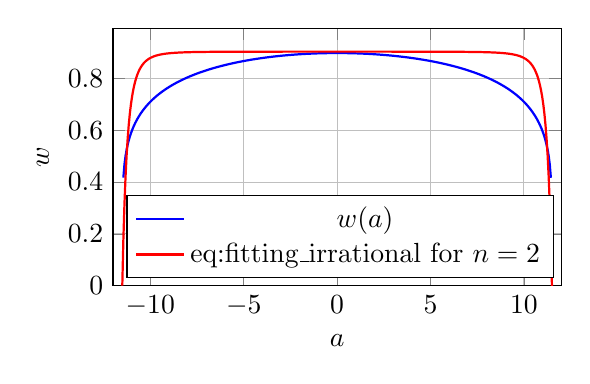
\begin{tikzpicture}
		\begin{axis}[
				xlabel={$a$},
				ylabel={$w$},
				width=0.6\textwidth,
				height=0.4\textwidth,
				grid=major,
				legend pos=south west,
				xmin=-12, xmax=12,
				ymin=0
			]
			\addplot[domain=-11.5:11.5,samples=400, blue, thick] { (1/14)*((51.282*sqrt(132.25 - x^2))^(1/3)) + (1/0.910)*(1.667*sqrt(132.25 - x^2))*((51.282*sqrt(132.25 - x^2))^(-2/3)) };
			\addlegendentry{$w(a)$}
			\addplot[domain=-11.5:11.5,samples=400,red, thick] { 0.9040595325562741-1/((abs(x)-12.525535603937156)^4) };
			\addlegendentry{\eqref{eq:fitting_irrational} for $n=2$}
		\end{axis}
	\end{tikzpicture}
	\caption{Plot of $w$ versus $a$ and its approximation.}
	\label{fig:w_vs_a}
\end{figure}

% \pgfkeys{/pgf/fpu=true}
The following figures \ref{fig:resulting_diamonds} visualize the friction circle \eqref{eq:friction_circle}, its tighter constraint
\eqref{eq:friction_circle_stricter} and the resulting diamond-shaped bounds for $v$ and $\delta$ for a fixed value of $a$.

\begin{figure}[h]
	\centering
	\begin{subfigure}{0.49\textwidth}
		\centering
		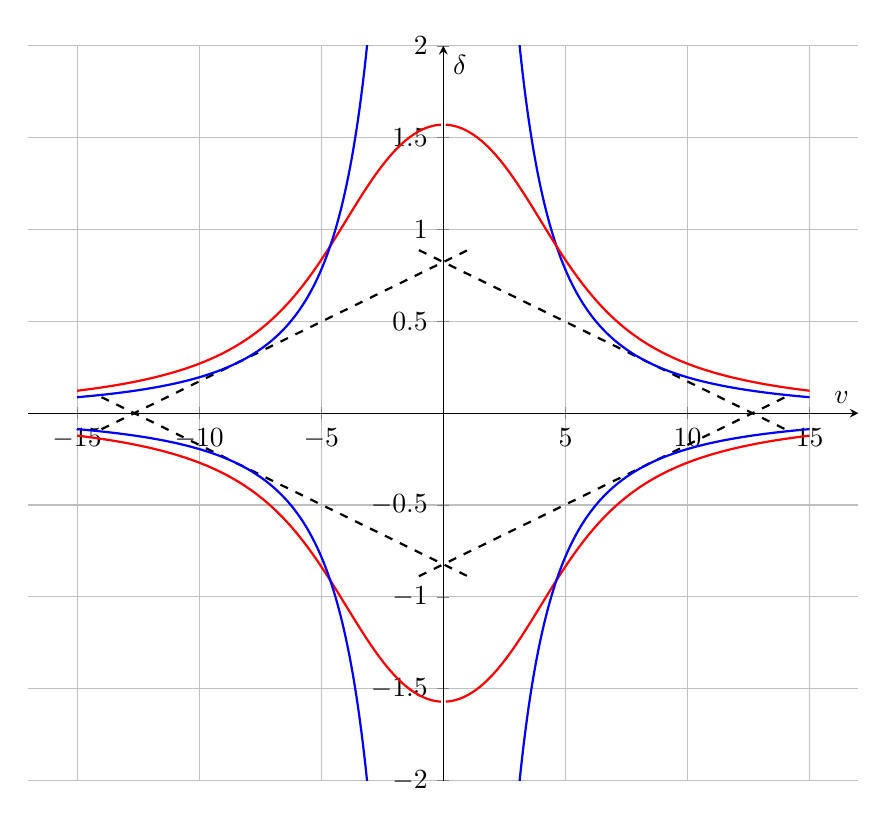
\begin{tikzpicture}
			\begin{axis}[
					xlabel={$v$},
					ylabel={$\delta$},
					width=\textwidth,
					height=0.9\textwidth,
					axis lines=middle,
					grid=major,
					legend pos=north west,
					xmin=-17, xmax=17,
					ymin=-2, ymax=2,
					legend to name=namedlegend, % Shared legend
					legend style={draw=none, cells={anchor=west}, font=\footnotesize},
				]

				% Define constants
				\def\vmax{14}
				\def\deltaMax{0.91}
				\def\lwb{2.4}
				\def\amax{11.5}
				\def\avar{0}

				% Diamond constraints
				\def\dv{1/\vmax}
				\def\ddelta{1/\deltaMax}
				\def\wvar{0.9040595325562741}

				\addplot[domain=-1:14, samples=400, dashed, thick, black]
				({x},{(\wvar-\dv*x )*\deltaMax});

				% Improved friction constraint
				\addplot[domain=2:15, samples=200, thick, blue]
				({x}, {sqrt(\amax^2 - \avar^2) * (1/(x^2)) * (\lwb * \deltaMax) / tan(\deltaMax r)});

				% Friction-circle constraints
				\addplot[domain=0.1:15, samples=200, thick, red]
				({x}, {rad(atan(\amax*\lwb/(x^2)))});

				\addplot[domain=-1:14, samples=400, dashed, thick, black]
				({x},{(\dv*x-\wvar )*\deltaMax});

				\addplot[domain=-14:1, samples=400, dashed, thick, black]
				({x},{(\wvar+\dv*x )*\deltaMax});

				\addplot[domain=-14:1, samples=400, dashed, thick, black]
				({x},{(-\wvar - \dv*x )*\deltaMax});

				% Friction-circle constraints
				\addplot[domain=0.1:15, samples=200, thick, red]
				({x}, {-rad(atan(\amax*\lwb/(x^2)))});

				\addplot[domain=-15:-0.1, samples=200, thick, red]
				({x}, {rad(atan(\amax*\lwb/(x^2)))});

				\addplot[domain=-15:-0.1, samples=200, thick, red]
				({x}, {-rad(atan(\amax*\lwb/(x^2)))});

				% Improved friction constraint
				\addplot[domain=-15:-2, samples=200, thick, blue]
				({x}, {sqrt(\amax^2 - \avar^2) * (1/(x^2)) * (\lwb * \deltaMax) / tan(\deltaMax r)});

				\addplot[domain=2:15, samples=200, thick, blue]
				({x}, {-sqrt(\amax^2 - \avar^2) * (1/(x^2)) * (\lwb * \deltaMax) / tan(\deltaMax r)});

				\addplot[domain=-15:-2, samples=200, thick, blue]
				({x}, {-sqrt(\amax^2 - \avar^2) * (1/(x^2)) * (\lwb * \deltaMax) / tan(\deltaMax r)});

				% Define legend
				\legend{Diamond Constraint, Tighter Friction Constraint, Friction Constraint}
			\end{axis}
		\end{tikzpicture}
		\caption{Plot of the resulting diamond at $a=0$.}
		\label{fig:resulting_diamond_0}
	\end{subfigure}
	\hfill
	\begin{subfigure}{0.49\textwidth}
		\centering
		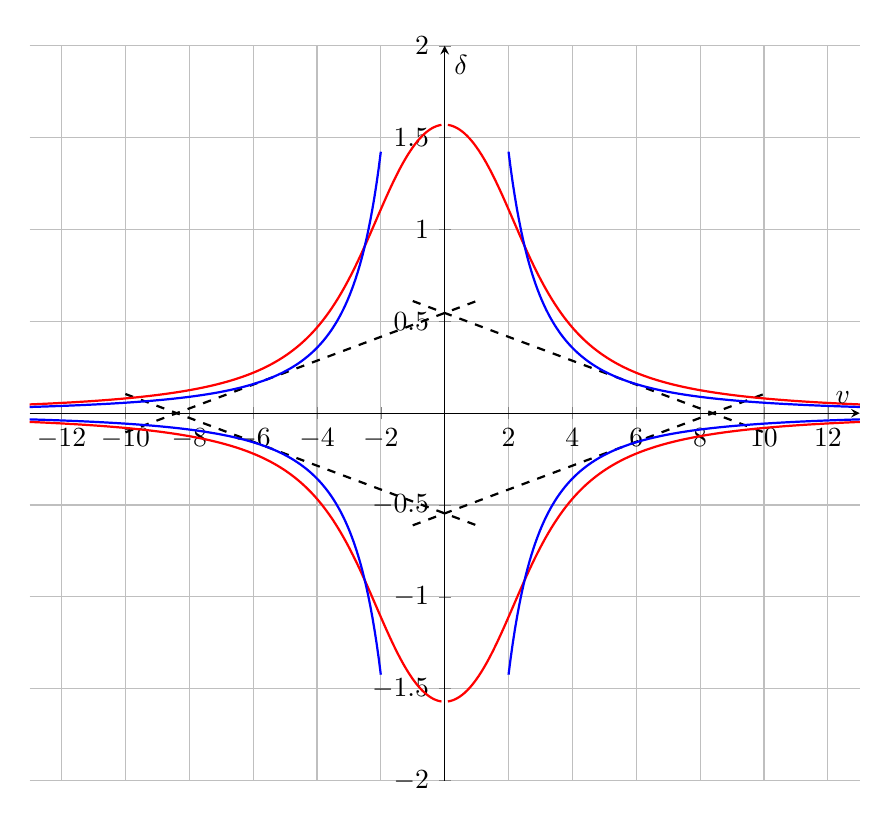
\begin{tikzpicture}
			\begin{axis}[
					xlabel={$v$},
					ylabel={$\delta$},
					width=\textwidth,
					height=0.9\textwidth,
					axis lines=middle,
					grid=major,
					legend pos=north west,
					xmin=-13, xmax=13,
					ymin=-2, ymax=2,
				]

				% Define constants
				\def\vmax{14}
				\def\deltaMax{0.91}
				\def\lwb{2.4}
				\def\amax{11.5}
				\def\avar{11}

				% Diamond constraints
				\def\dv{1/\vmax}
				\def\ddelta{1/\deltaMax}
				\def\wvar{0.5995469115149037}

				\addplot[domain=-1:10, samples=400, dashed, thick, black]
				({x},{(\wvar-\dv*x )*\deltaMax});

				\addplot[domain=-1:10, samples=400, dashed, thick, black]
				({x},{(\dv*x-\wvar )*\deltaMax});

				\addplot[domain=-10:1, samples=400, dashed, thick, black]
				({x},{(\wvar+\dv*x )*\deltaMax});

				\addplot[domain=-10:1, samples=400, dashed, thick, black]
				({x},{(-\wvar - \dv*x )*\deltaMax});

				% Friction-circle constraints
				\addplot[domain=0.1:15, samples=200, thick, red]
				({x}, {rad(atan(sqrt(\amax^2 - \avar^2)*\lwb/(x^2)))});

				\addplot[domain=0.1:15, samples=200, thick, red]
				({x}, {-rad(atan(sqrt(\amax^2 - \avar^2)*\lwb/(x^2)))});

				\addplot[domain=-15:-0.1, samples=200, thick, red]
				({x}, {rad(atan(sqrt(\amax^2 - \avar^2)*\lwb/(x^2)))});

				\addplot[domain=-15:-0.1, samples=200, thick, red]
				({x}, {-rad(atan(sqrt(\amax^2 - \avar^2)*\lwb/(x^2)))});

				% Improved friction constraint
				\addplot[domain=2:15, samples=200, thick, blue]
				({x}, {sqrt(\amax^2 - \avar^2) * (1/(x^2)) * (\lwb * \deltaMax) / tan(\deltaMax r)});

				\addplot[domain=-15:-2, samples=200, thick, blue]
				({x}, {sqrt(\amax^2 - \avar^2) * (1/(x^2)) * (\lwb * \deltaMax) / tan(\deltaMax r)});

				\addplot[domain=2:15, samples=200, thick, blue]
				({x}, {-sqrt(\amax^2 - \avar^2) * (1/(x^2)) * (\lwb * \deltaMax) / tan(\deltaMax r)});

				\addplot[domain=-15:-2, samples=200, thick, blue]
				({x}, {-sqrt(\amax^2 - \avar^2) * (1/(x^2)) * (\lwb * \deltaMax) / tan(\deltaMax r)});
			\end{axis}
		\end{tikzpicture}
		\caption{Plot of the resulting diamond at $a=11$.}
		\label{fig:resulting_diamond_1}
	\end{subfigure}
	% Shared legend
	\ref{namedlegend}
	\caption{Comparison of the resulting diamond constraints for different acceleration values.}
	\label{fig:resulting_diamonds}
\end{figure}

In conclusion, this approach constructs a convex approximation of the friction circle and allows for weighting either $v$ or $\delta$ by setting
$v^*$.
The final constraint can be stated as follows:
\begin{equation}
	a^2 + (\frac{1}{l_{wb}}\frac{\tan(\delta^*)}{\delta^*})^2 w \leq a_{max}^2
	\label{eq:final_friction_circle}
\end{equation}
where $w$ is new introduced auxiliary variable, which is bounded by:
\begin{equation}
	0 \leq w \leq \tilde{w}(a)
	\label{eq:final_friction_circle_bounds}
\end{equation}
Our final model is now complete and ready for use in the optimization process.
It is represented by the tuple
\begin{equation}
	M_{kst}=(x_{kst}, u_{kst}, \tilde{f}_{kst}, \{w_{v,\xi}, w_{v,\delta}, w_{s,\dot{s}}, w\}, C) \label{model:kst} \end{equation} where $C$ consists of
the coupling constraints \eqref{eq:coupling_kst_0}, \eqref{eq:coupling_kst_1}, the McCormick bounds \eqref{fig:mccormick_constraints}, the introduced
hyperplanes \eqref{eq:first_hyperplane}-\eqref{eq:last_hyperplane}, and our approximated friction circle \eqref{eq:final_friction_circle} with
\eqref{eq:final_friction_circle_bounds}.

% \subsection{Linearize Quadratic Term}

% In this section, we will linearize the quadratic term $s^2$ in the state transition model.
% For quadratic terms, which occur in equality constraints, we can use the McCormick relaxation technique, which is typically used for bilinear terms,
% but can also be applied to quadratic terms.
% However, in the case of quadratic terms, we can achieve better bounds.
% For the lower bound, which must be convex, we can simply use the term itself, as a quadratic term is always convex.
% The best upper bound can be obtained by connecting the points defined by the bounds on $s$.
% \[
% 	s^2 \leq (\underline{s} + \overline{s})s - \underline{s}\overline{s}
% \]

\section{Modeling Techniques} \label{ch:modeling_techniques}

In the previous chapters, we have explored various modeling techniques that are essential for solving complex optimization problems.
We began by discussing the decoupling of variables using quantifier elimination, a powerful method that simplifies the problem by reducing the number
of variables involved.
This technique is particularly useful in scenarios where the relationships between variables are intricate and non-linear.

Next, we examined convex relaxations, specifically focusing on McCormick envelopes for bilinear terms.
Convex relaxations are important for transforming non-convex problems into convex ones, which are easier to solve.
McCormick envelopes provide a way to approximate bilinear terms with convex functions, thereby enabling the use of efficient convex optimization
algorithms.

In this section, we present a collection of commonly used modeling methods for convex programming.
These methods serve as a practical guide for formulating and solving convex optimization problems.

\subsection{Soft Constraints}

Soft constraints are used in optimization problems where certain constraints can be violated to some extent, but with a penalty.
This is in contrast to hard constraints, which must be strictly satisfied.
Soft constraints are particularly useful in real-world scenarios where it is often impractical to meet all constraints perfectly.

To incorporate soft constraints into a convex optimization problem, we introduce slack variables and a penalty term in the objective function.
The slack variables measure the extent of constraint violation, and the penalty term ensures that violations are minimized.

Consider a constraint of the form \( g(x) \leq 0 \).
To make this constraint soft, we introduce a slack variable \( s \geq 0 \) and modify the constraint to \( g(x) \leq s \).
We then add a penalty term \( \lambda s \) to the objective function, where \( \lambda \) is a positive weight that controls the trade-off between
minimizing the original objective and satisfying the constraint.

The modified optimization problem can be written as:
\begin{align*}
	\min_{x, s} \quad       & f(x) + \lambda s \\
	\text{subject to} \quad & g(x) \leq s      \\
	                        & s \geq 0
\end{align*}

By adjusting the value of \( \lambda \), we can control the degree to which the soft constraint is enforced.
A larger \( \lambda \) places more emphasis on satisfying the constraint, while a smaller \( \lambda \) allows for greater flexibility in violating
the constraint.

\subsection{Auxiliary Variables}

Auxiliary variables can be used for modeling in many ways.
In our models we are the defining the road with as a function over $s$ the distance along the road.
One common part objective may be to minimize the offset to the center of the road.
The first formulation that may come to mind is: \[ \min g(x, u) + \left( n - \frac{\overline{n}(s) - \underline{n}(s)}{2} \right) \] This is a valid
formulation, but it is not convex.
Instead, we are using different approach to formulate the offset to the center of the road.
\[
	\min \left\{ \overline{n}(s) - n, n - \underline{n}(s) \right\}
\]
which gives us the distance to the closer boundary of the road.
This formulation is concave, if $\overline{n}(s)$ is concave and $\underline{n}(s)$ is convex.
By introducing the auxiliary variable $d$ which is constrained by: \[ 0 \leq d \leq \min \left\{ \overline{n}(s) - n, n - \underline{n}(s) \right\}
\] we can reformulate the objective as: \[ \min g(x, u) - d^2 \] This formulation is convex and can be solved efficiently.

To visualize these formulations, we can plot them using a constant value for \(\overline{n}(s)\) and \(\underline{n}(s)\).
Let's assume \(\overline{n}(s) = 5\) and \(\underline{n}(s) = 1\).

\begin{figure}[H]
	\centering
	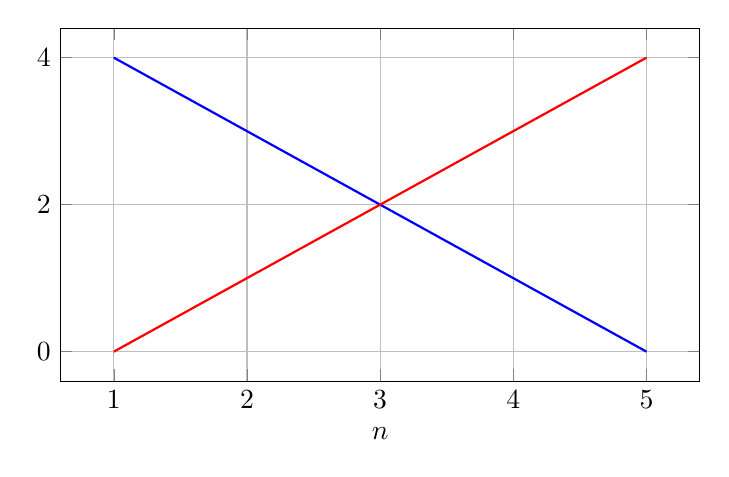
\begin{tikzpicture}
		\begin{axis}[
				xlabel={$n$},
				legend pos=outer north east,
				grid=major,
				width=0.8\textwidth,
				height=0.5\textwidth
			]
			\addplot[domain=1:5, samples=100, thick, blue] {5-x};
			\addplot[domain=1:5, samples=100, thick, red] {x-1};
		\end{axis}
	\end{tikzpicture}
	\caption{Plot of distance to road boundaries}
	\label{fig:road_boundaries}
\end{figure}

In this plot \ref{fig:road_boundaries}, the blue line represents \(\overline{n}(s) - n\), the red line represents \(n - \underline{n}(s)\).

We can also plot the objective function for the new formulation.

\begin{figure}[H]
	\centering
	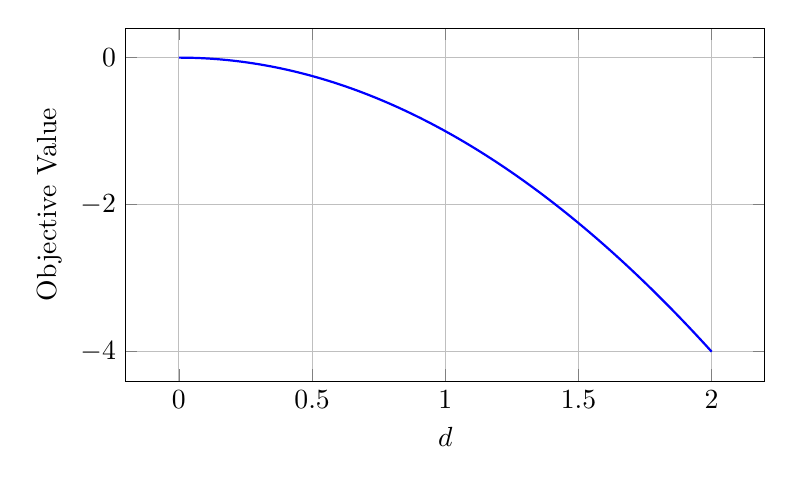
\begin{tikzpicture}
		\begin{axis}[
				xlabel={$d$},
				ylabel={Objective Value},
				legend pos=outer north east,
				grid=major,
				width=0.8\textwidth,
				height=0.5\textwidth
			]
			\addplot[domain=0:2, samples=100, thick, blue] {-x^2};
		\end{axis}
	\end{tikzpicture}
	\caption{Plot of the objective function}
	\label{fig:objective_functions}
\end{figure}

While \(-\min(5 - x, x - 1)\) is a convex function, it is piece wise linear, which can lead to difficulties in optimization.
The benefit of using an auxiliary variable in this context is that it allows us to transform a piece wise linear and potentially non-differentiable
objective function into a smooth and differentiable convex function.
This transformation simplifies the optimization process, making it more efficient and reliable.
Specifically, by introducing the auxiliary variable \( d \) and reformulating the objective as \(\min g(x, u) - d^2\), we obtain a function that is
easier to handle with gradient-based optimization algorithms, which rely on smoothness and differentiability to find optimal solutions effectively.

\subsection{Penalty Methods}

Penalty methods are another approach to handle constraints in optimization problems.
These methods incorporate constraints into the objective function by adding a penalty term that increases the objective value when constraints are
violated.
This approach transforms a constrained optimization problem into an unconstrained one, which can be easier to solve.

Consider an optimization problem with a constraint \( g(x) \leq 0 \).
In a penalty method, we modify the objective function to include a penalty term \( P(g(x)) \) that penalizes constraint violations.
A common choice for the penalty term is a quadratic function, such as \( P(g(x)) = \mu \max(0, g(x))^2 \), where \( \mu \) is a positive penalty
parameter.

The modified optimization problem can be written as:
\begin{align*}
	\min_{x} \quad & f(x) + \mu \max(0, g(x))^2
\end{align*}

By adjusting the value of \( \mu \), we can control the severity of the penalty for constraint violations.
A larger \( \mu \) places more emphasis on satisfying the constraint, while a smaller \( \mu \) allows for greater flexibility in violating the
constraint.

Penalty methods are particularly useful when dealing with complex constraints that are difficult to handle directly.
By incorporating these constraints into the objective function, we can leverage efficient unconstrained optimization algorithms to find solutions.

\subsection{Lagrangian Relaxation}

Lagrangian relaxation is a technique used to simplify complex optimization problems by relaxing some of the constraints and incorporating them into
the objective function using Lagrange multipliers.
This approach transforms the original problem into a simpler one that can be solved more easily.

Consider an optimization problem with a constraint \( g(x) \leq 0 \).
In Lagrangian relaxation, we introduce a Lagrange multiplier \( \lambda \geq 0 \) and form the Lagrangian function:
\[
	L(x, \lambda) = f(x) + \lambda g(x)
\]

The relaxed optimization problem can be written as:
\begin{align*}
	\min_{x} \quad          & L(x, \lambda)  \\
	\text{subject to} \quad & \lambda \geq 0
\end{align*}

By solving the relaxed problem for different values of \( \lambda \), we can obtain a lower bound on the optimal value of the original problem.
The quality of the bound depends on the choice of \( \lambda \), and finding the best value of \( \lambda \) is an optimization problem in itself.

Lagrangian relaxation is particularly useful in combinatorial optimization problems, where it can provide strong bounds and guide the search for
optimal solutions.
It is also a key component of more advanced techniques, such as the Lagrangian duality and the subgradient method.

\subsection{Conclusion}

In this chapter, we have explored various modeling techniques that are essential for solving complex optimization problems.
We discussed the use of soft constraints, auxiliary variables, penalty methods, and Lagrangian relaxation, each of which offers unique advantages for
handling different types of constraints and objectives.
By understanding and applying these techniques, we can formulate and solve optimization problems more effectively, leading to better solutions and
improved performance in practical applications.


\chapter{Evaluation}
\chapter{Kinematic Single Track Model in Frenet Frame}

We have already introduced the kinematic single track model in which a steering angle and an orientation, which will now combine with the idea of the
previous chapter.
We want to model our state variables in the road aligned frame, which is the Frenet frame.
The states and controls variables of the kinematic single track model are defined in the global coordinate system are defined as in \ref{eq:states_kst} and \ref{eq:controls_kst}:

\begin{figure}[h]
	\centering
	\begin{subfigure}[b]{0.45\textwidth}
		\centering
		$x = \begin{bmatrix} p_x \\ p_y \\ \delta \\ v \\ \psi \end{bmatrix}$
		\caption{State Variables}
	\end{subfigure}
	\hfill
	\begin{subfigure}[b]{0.45\textwidth}
		\centering
		$u = \begin{bmatrix} v_{\delta} \\ a_{\text{long}} \end{bmatrix}$
		\caption{Control Inputs}
	\end{subfigure}
\end{figure}

Our goal is not model dynamics and state variables in the Frenet frame.

\section{Implementation Details} \label{sec:implementation_details}

For our evaluation, we need to determine the road segment for each time point, configure our solver to solve the optimization problem, and provide
the time points $\{t_i\}_{i=1,\dots,n}$.

\subsection{Road Segments}

For our double integrator model, we want to split up the road into segments, based on mainly their curvature.
As already discussed this approach allows the model to have a larger search space during planning.
The introduced kinematic single track model assumes the curvature to be linear, which is only practical for the road topology if we allow a piece
wise linear curvature and select the current piece.
We can easily add other road topology constraints to be dependent by the current segment, such as the road width.

Our planner operates on a time horizon, divided into discrete time steps $\{t_i\}_{i=1,\dots,n}$.
For each time point, we seek the state and the transition to the next time point, controlled by the input.
The transition is constrained by the dynamics of the model, the state variables, and the control input through coupling constraints.
To make the dynamics and coupling constraints dependent on the road segment, we need to provide the current road segment for each time point.

Given the start and end of each road segment $\{[s_{i-1}, s_{i}]\}_{i=1,\dots,m}$ and the current position $s$ of the vehicle, with a reference velocity
$v(t)$ which can be time-dependent, we can determine the current road segment for each time point by:
\begin{equation}
	i_{s, \{s_{i}\}_{i=0,\dots,m}, v}: \{t_i\}_{i=1,\dots,n} \to \{1,\dots,m\}, t \mapsto i(t) = \min \left\{ j \mid s + \int_{0}^{t} v(\sigma) d\sigma \leq s_j \right\}
\end{equation}

This function can be used to determine the road segment-dependent variables.
We want to make not only the curvature road segment-dependent but also the road width.
The road width consists of the left $\overline{n}(s)$ and right $\underline{n}(s)$ lane width.
The left lane width can be concave, and the right lane width can be convex.
Thus, our implementation of a road segment includes a linear curvature, a concave and convex lane width, and the length of the segment.
This can be extended to include, for example, the upper velocity limits for each segment.

\subsection{Planner}

The convex discrete-time optimization problem will be solved using an external solver, which we refer to as the planner, as it provides the solution
to the motion planning problem.
Our trajectory planner is parameterized by a tuple $(\text{dim}(x), \text{dim}(u), f, \mathcal{C})$, which includes the dimensions of the state
variables, the dimensions of the control inputs, the dynamics equation represented by $f$, and the coupling constraints represented by $\mathcal{C}$.
The time horizon and discretization are given by $\{t_i\}_{i=0,\dots,n}$.

To construct the variables and constraints for our planner, we need to define the state variables, control inputs, and the constraints that describe
the transitions between states.

First, we define the state variables and control inputs for each time step $t_i$:
\begin{equation}
	x(t_i) \in \mathbb{R}^{dim(x)}, u(t_i) \in \mathbb{R}^{dim(u)}
\end{equation}

The system dynamics differ based on the chosen model:

\textbf{Double Integrator Model:} Given the exact discretization of the double integrator
model in \eqref{eq:discrete_time_dynamics_di}, we define the system dynamics constraint as:
\begin{equation}
	x(t_i) = f_{d,di}(x(t_{i-1}), u(t_{i-1}), t_i - t_{i-1})
\end{equation}
\textbf{Bicycle Model:}
Since the dynamics of the kinematic bicycle model include auxiliary variables, we apply forward Euler discretization to the continuous-time dynamics:
\begin{equation}
	x(t_i) = x(t_{i-1}) + \tilde{f}_{kst}(x(t_{i-1}), u(t_{i-1})) \cdot (t_i - t_{i-1})
\end{equation}
where $\tilde{f}_{kst}$ is defined in \eqref{eq:kst_final_dynamics}.

These system dynamics, combined with the coupling constraints and additional constraints, define the full set of variables and constraints used by
the planner.

Given the initial state $x_{initial}$, we model our initial condition with the constraint $x(t_0) = x_{initial}$.
For our evaluation, we did not impose any additional constraints on the final state.
Instead, we modeled our driving behavior through the objective function.

We implemented our optimization problem using Python with the 'cvxpy' library and solved it using the 'MOSEK' solver.

While our planner primarily relies on hard constraints to ensure feasibility and adherence to system dynamics, real-world scenarios often introduce
uncertainties, disturbances, or conflicting objectives that make strict constraint satisfaction impractical.
To address this, we incorporate soft constraints, which allow for controlled constraint relaxation in exchange for a penalty.
By integrating soft constraints into the optimization framework, we can balance feasibility with optimality, enabling more flexible and robust motion
planning.

\subsection{Soft Constraints}

Soft constraints are used in optimization problems where certain constraints can be violated to some extent, but with a penalty.
This is in contrast to hard constraints, which must be strictly satisfied.
Soft constraints are particularly useful in real-world scenarios where it is often impractical to meet all constraints perfectly.

To incorporate soft constraints into a convex optimization problem, we introduce slack variables and a penalty term in the objective function.
The slack variables measure the extent of constraint violation, and the penalty term ensures that violations are minimized.

Consider a constraint of the form \( g(x) \leq 0 \).
To make this constraint soft, we introduce a slack variable \( s \geq 0 \) and modify the constraint to \( g(x) \leq s \).
We then add a penalty term \( \lambda s \) to the objective function, where \( \lambda \) is a positive weight that controls the trade-off between
minimizing the original objective and satisfying the constraint.

The modified optimization problem can be written as:
\begin{align*}
	\min_{x, s} \quad       & f(x) + \lambda s \\
	\text{subject to} \quad & g(x) \leq s      \\
	                        & s \geq 0
\end{align*}

By adjusting the value of \( \lambda \), we can control the degree to which the soft constraint is enforced.
A larger \( \lambda \) places more emphasis on satisfying the constraint, while a smaller \( \lambda \) allows for greater flexibility in violating
the constraint.

\subsection{Replanning Strategy}

In our simulation, we employed a replanning strategy to implement a feedback mechanism.
In addition to the time horizon, we implemented a fixed time interval, shorter than the time horizon, after which the planner recalculates the
trajectory from the current position of the vehicle.
This replanning mechanism allows the planner to adjust to changes in the environment or deviations from the planned path.
We employed a time discretization of equal intervals for the replanning time interval, and the time intervals increase linearly for the remaining
time horizon.

\begin{figure}[h]
	\centering
	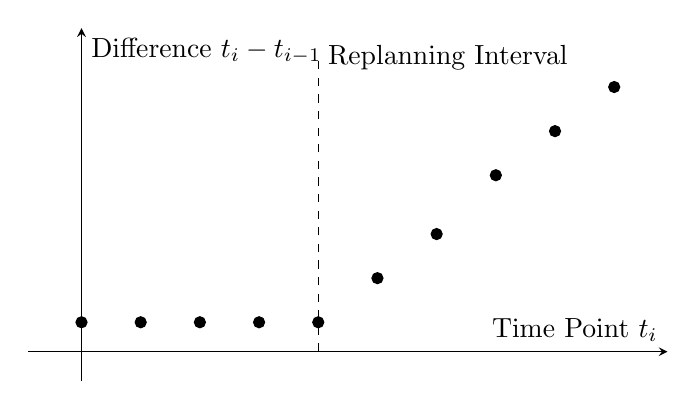
\begin{tikzpicture}
		\begin{axis}[
				xlabel={Time Point $t_i$},
				ylabel={Difference $t_i - t_{i-1}$},
				width=0.8\textwidth,
				height=0.5\textwidth,
				grid=major,
				axis lines=middle,
				enlargelimits=true,
				xtick=\empty, % Remove x-axis ticks
				ytick=\empty, % Remove y-axis ticks
				clip=false
			]
			% Data points
			\addplot[only marks, mark=*, mark size=2pt]
			coordinates {
					(0,0.2) (1,0.2) (2,0.2) (3,0.2) (4,0.2) (5,0.5) (6,0.8) (7,1.2) (8,1.5) (9,1.8)
				};

			% Dashed vertical line for replanning interval
			\addplot[dashed] coordinates {(4,0) (4,2)};

			% Replanning label
			\node[anchor=west] at (axis cs:4,2) {Replanning Interval};

		\end{axis}
	\end{tikzpicture}
	\caption{Time points and their differences to previous time points}
	\label{fig:time_points}
\end{figure}

Figure \ref{fig:time_points} illustrates the time points and their intervals.
The states for the time points to the left of the dashed line are simulated, after which a replanning is triggered.
This replanning follows the same time discretization pattern as the initial planning phase.
The term $\Delta t$ refers to the time intervals between the initial time points, which vary across the different benchmark scenarios.
The slope of time difference after the replanning interval is given by $\Delta^2 t_{replan}$.

Next, we introduce our benchmarking framework, consisting of configurations, such as objectives, road.

\section{Performance Evaluation} \label{sec:performance-evaluation}

\subsection{Objectives} \label{subsec:objectives}

Our trajectory planner aims to minimize a cost function that represents the driving behavior we desire.
The cost function is composed of several objectives, each weighted by a corresponding factor.

The primary objectives considered are control effort, deviation from the reference trajectory, and terminal state accuracy.
The control effort objective aims to minimize
the numerical derivatives of control inputs to ensure smooth driving, represented by the cost function:
\begin{equation}
	J_{control} = \sum_{i=0}^{n-1} \left\| d_1(t_i) \right\|^2
\end{equation}
where $d_1(t_i)\in \mathbb{R}^{dim(u)}$ is an auxiliary variable constrained by: \[
	d_1(t_i) = \frac{u(t_i) - u(t_{i-1})}{t_i - t_{i-1}}
\]

The tracking objective aims to minimize the deviation from the center of the road, represented by the cost function:
\begin{equation}
	J_{tracking} = \sum_{i=0}^{n} d_2(t_i)^2 \end{equation} where $d_2(t_i)\in \mathbb{R}$ is an auxiliary variable representing the negative distance to
the closest boundary, constrained by: \[ \max \left\{ n(t_i)-\overline{n}(s(t_i)), \underline{n}(s(t_i)) - n(t_i) \right\} \leq d_2(t_i)\] By
minimizing $J_{tracking}$, we maximize the distance to the road boundaries, which is optimal when the vehicle is centered on the road.

The terminal state objective aims to minimize the deviation from a desired terminal state $x_{final}$ at the final time step $t_n$, represented by the cost function:
\begin{equation}
	J_{terminal} = \|x(t_n) - x_{final}\|^2
\end{equation}

The total cost function $J$ is a weighted sum of these objectives:
\begin{equation}
	J = \alpha J_{control} + \beta J_{tracking} + \gamma J_{terminal} \label{eq:cost_function_combined} \end{equation} where $\alpha$, $\beta$, and
$\gamma$ are the weights that determine the relative importance of each objective.
By minimizing this cost function, our trajectory planner generates a trajectory that balances control effort, tracking the reference trajectory, and
accuracy in reaching the desired terminal state.

Since some of our objectives, such as $J_{tracking}$, involve nonlinear or nonconvex formulations, directly incorporating them into the optimization
problem can be challenging.
To address this, we introduce auxiliary variables that allow us to reformulate certain objectives into convex, computationally efficient expressions.
These auxiliary variables help model constraints and cost functions in a way that preserves convexity while maintaining the intended optimization
behavior.

\subsubsection{Auxiliary Variables}

Auxiliary variables can be used for modeling in many ways.
In our models we are the defining the road with as a function over $s$ the distance along the road.
One common part objective may be to minimize the offset to the center of the road.
The first formulation that may come to mind is: \[ \min g(x, u) + \left( n - \frac{\overline{n}(s) - \underline{n}(s)}{2} \right)^2 \] This is a
valid formulation, but it is not convex.
Instead, we are using different approach to formulate the offset to the center of the road.
\[
	\max \left\{ n - \overline{n}(s),  \underline{n}(s) - n \right\}
\]
which gives us the negative distance to the closer boundary of the road.
This formulation is convex, if $\overline{n}(s)$ is concave and $\underline{n}(s)$ is convex.
By introducing the auxiliary variable $d$ which is constrained by: \[ \max \left\{ n - \overline{n}(s), \underline{n}(s) - n \right\} \leq d \] we
can reformulate the objective as: \[ \min g(x, u) + d^2 \] This formulation is convex and can be solved efficiently.

To visualize these formulations, we can plot them using a constant value for \(\overline{n}(s)\) and \(\underline{n}(s)\) in Figure
\ref{fig:auxiliary_variables}.
Let's assume \(\overline{n}(s) = 5\) and \(\underline{n}(s) = 1\).

\begin{figure}[H]
	\centering
	\begin{subfigure}{0.48\textwidth}
		\centering
		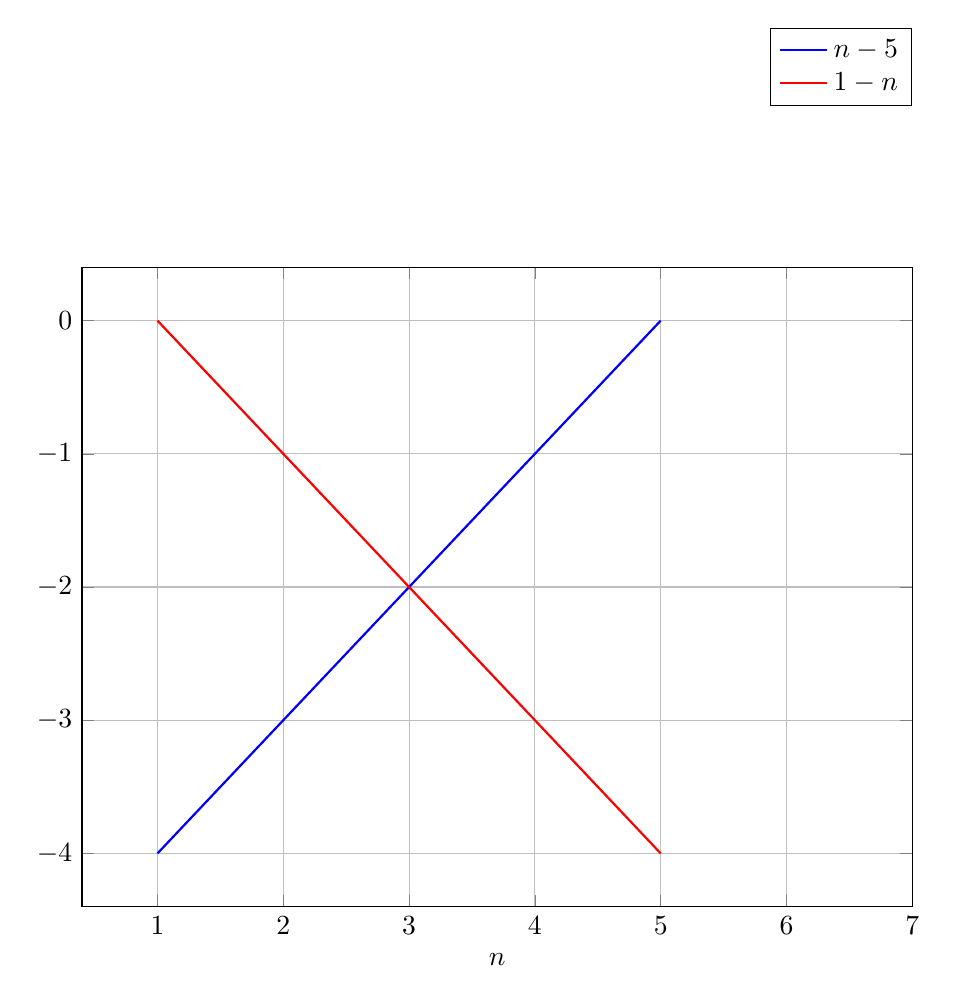
\begin{tikzpicture}
			\begin{axis}[
					xlabel={$n$},
					legend style={at={(axis cs:7,2.2)},anchor=north east},
					grid=major,
					width=\textwidth,
					height=0.8\textwidth,
					xmax=7,
				]
				\addplot[domain=1:5, samples=100, thick, blue] {x-5};
				\addplot[domain=1:5, samples=100, thick, red] {1-x};
				\legend{$n - 5$, $1-n$}
			\end{axis}
		\end{tikzpicture}
		\caption{Negative Distance to Road Boundaries}
		\label{fig:road_boundaries}
	\end{subfigure}
	\hfill
	\begin{subfigure}{0.48\textwidth}
		\centering
		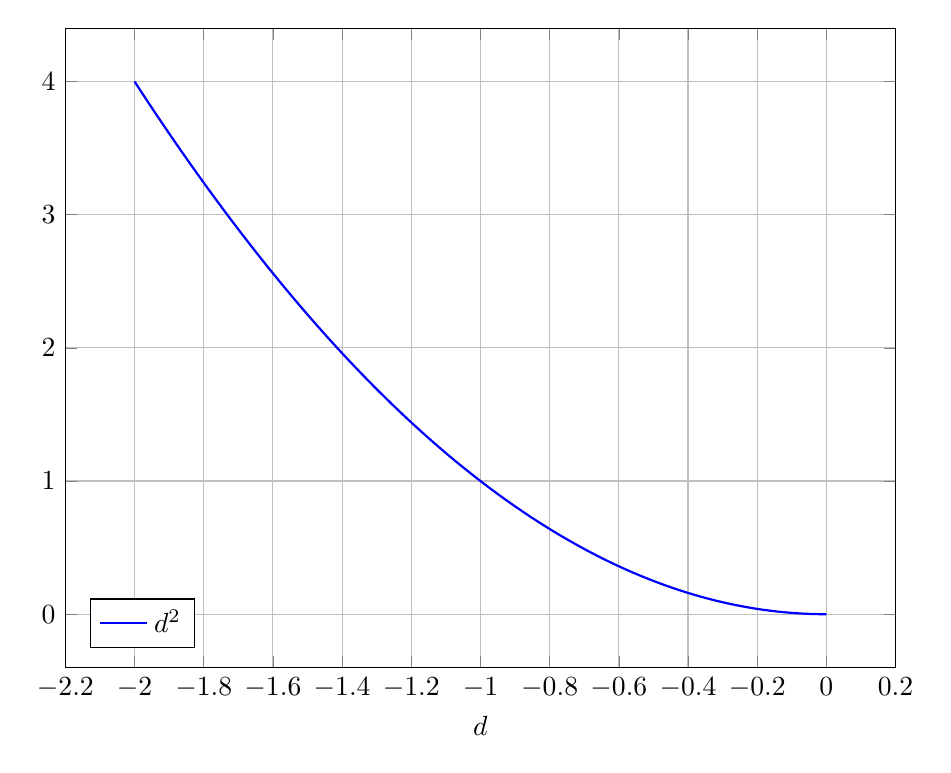
\begin{tikzpicture}
			\begin{axis}[
					xlabel={$d$},
					legend pos=south west,
					grid=major,
					width=\textwidth,
					height=0.8\textwidth
				]
				\addplot[domain=-2:0, samples=100, thick, blue] {x^2};
				\legend{$d^2$}
			\end{axis}
		\end{tikzpicture}
		\caption{Objective Function}
		\label{fig:objective_functions}
	\end{subfigure}
	\caption{Plots the distance to the road boundaries and the objective function.}
	\label{fig:auxiliary_variables}
\end{figure}

While \(\max(x-5, 1-x)\) is a convex function, it is piecewise linear, which can lead to difficulties in optimization.
The benefit of using an auxiliary variable in this context is that it allows us to transform a piecewise linear and potentially non-differentiable
objective function into a smooth and differentiable convex function.
This transformation simplifies the optimization process, making it more efficient and reliable.
Specifically, by introducing the auxiliary variable \( d \) and reformulating the objective as \(\min g(x, u) + d^2\), we obtain a function that is
easier to handle with gradient-based optimization algorithms, which rely on smoothness and differentiability to find optimal solutions effectively.

\subsection{Scenarios} \label{subsec:scenarios}

In order to evaluate the performance of our trajectory planner, we implemented several driving scenarios.
These scenarios are designed to test different aspects of the planner's capabilities.
The Straight Road scenario evaluates the planner's ability to maintain a straight path with minimal control effort, ensuring smooth and efficient
driving.
In the Left Turn scenario, the planner's performance is assessed based on its ability to execute a smooth left turn while adhering to the reference
trajectory.
The Lane Change scenario tests the planner's capability to perform a lane change maneuver safely and efficiently, highlighting its responsiveness and
precision.
The Slalom scenario challenges the planner to navigate through a series of closely spaced obstacles, requiring precise control and smooth transitions
between maneuvers.
The Elchtest, also known as the moose test, evaluates the planner's ability to perform a sudden evasive maneuver to avoid an obstacle, testing its
quick decision-making and control under pressure.
The Elchtest scenario can be visualized as follows:
\begin{figure}[H]
	\centering
	\begin{tikzpicture}
		\draw[thick, dashed] (0,-0.5) -- (5,-0.5); % Road boundary
		\draw[thick, dashed] (0,0.5) -- (3,0.5); % Road boundary
		\draw[thick, dashed] (3,0.5) -- (3,1.5); % Road boundary
		\draw[thick, dashed] (5,0.5) -- (5,-0.5); % Road boundary
		\draw[thick, dashed] (5,0.5) -- (7,0.5); % Road boundary
		\draw[thick, dashed] (3,1.5) -- (9,1.5); % Road boundary
		\draw[thick, dashed] (9,0.5) -- (9,1.5); % Road boundary
		\draw[thick, dashed] (7,0.5) -- (7,-0.5); % Road boundary
		\draw[thick, dashed] (7,-0.5) -- (12,-0.5); % Road boundary
		\draw[thick, dashed] (9,0.5) -- (12,0.5); % Road boundary
		\node at (0,0) {Start};
		\node at (12,0) {End};
	\end{tikzpicture}
	\caption{Elchtest scenario visualization}
	\label{fig:elchtest}
\end{figure}

Finally, the Sharp U Turn scenario tests the planner's ability to execute a sharp U-turn, challenging its control effort and adherence to the desired
terminal state.

By evaluating the planner in these diverse scenarios, we can gain a comprehensive understanding of its strengths and areas for improvement.

\begin{longtable}{l c c c c c}
	\caption{Overview of Road Segments and Their Properties}                                                                                             \\
	\toprule
	\textbf{Road Name}                & \textbf{Segment} & \textbf{Length} & \textbf{Curvature} & \multicolumn{2}{c}{\textbf{Lane Width}}                \\
	\cmidrule(lr){5-6}
	                                  &                  &                 &                    & \textbf{Start}                          & \textbf{End} \\
	\midrule
	\endfirsthead

	\multicolumn{6}{c}{\textit{Continued from previous page}}                                                                                            \\
	\toprule
	\textbf{Road Name}                & \textbf{Segment} & \textbf{Length} & \textbf{Curvature} & \multicolumn{2}{c}{\textbf{Lane Width}}                \\
	\cmidrule(lr){5-6}
	                                  &                  &                 &                    & \textbf{Start}                          & \textbf{End} \\
	\midrule
	\endhead

	\bottomrule
	\multicolumn{6}{c}{\textit{Continued on next page}}                                                                                                  \\
	\endfoot

	\bottomrule
	\endlastfoot

	\multirow{5}{*}{Elchtest}         & 1                & 12.0            & 0.000              & [-1.0,1.0]                              & [-1.0,1.0]   \\
	                                  & 2                & 13.5            & 0.000              & [-1.0,1.0]                              & [2.0,4.7]    \\
	                                  & 3                & 11.0            & 0.000              & [2.0,4.7]                               & [2.0,4.7]    \\
	                                  & 4                & 12.5            & 0.000              & [2.0,4.7]                               & [-1.0,1.0]   \\
	                                  & 5                & 12.0            & 0.000              & [-1.0,1.0]                              & [-1.0,1.0]   \\
	\midrule
	\multirow{1}{*}{Left Turn}        & 1                & 235.6           & 0.007              & [-2.0,2.0]                              & [-2.0,2.0]   \\
	\midrule
	\multirow{1}{*}{Straight}         & 1                & 180.0           & 0.000              & [-2.0,2.0]                              & [-2.0,2.0]   \\
	\midrule
	\multirow{4}{*}{Lane Change}      & 1                & 30.0            & 0.000              & [-2.0,2.0]                              & [-2.0,2.0]   \\
	                                  & 2                & 20.9            & 0.025              & [-2.0,2.0]                              & [-2.0,2.0]   \\
	                                  & 3                & 20.9            & -0.025             & [-2.0,2.0]                              & [-2.0,2.0]   \\
	                                  & 4                & 30.0            & 0.000              & [-2.0,2.0]                              & [-2.0,2.0]   \\
	\midrule
	\multirow{5}{*}{Slalom}           & 1                & 20.0            & 0.000              & [-2.0,2.0]                              & [-2.0,2.0]   \\
	                                  & 2                & 94.2            & -0.033             & [-2.0,2.0]                              & [-2.0,2.0]   \\
	                                  & 3                & 94.2            & 0.033              & [-2.0,2.0]                              & [-2.0,2.0]   \\
	                                  & 4                & 94.2            & -0.033             & [-2.0,2.0]                              & [-2.0,2.0]   \\
	                                  & 5                & 20.0            & 0.000              & [-2.0,2.0]                              & [-2.0,2.0]   \\
	\midrule
	\multirow{3}{*}{Feasible Curve}   & 1                & 20.0            & 0.000              & [-2.0,2.0]                              & [-2.0,2.0]   \\
	                                  & 2                & 15.7            & 0.200              & [-2.0,2.0]                              & [-2.0,2.0]   \\
	                                  & 3                & 20.0            & 0.000              & [-2.0,2.0]                              & [-2.0,2.0]   \\
	\midrule
	\multirow{3}{*}{Infeasible Curve} & 1                & 20.0            & 0.000              & [-2.0,2.0]                              & [-2.0,2.0]   \\
	                                  & 2                & 8.8             & 0.357              & [-2.0,2.0]                              & [-2.0,2.0]   \\
	                                  & 3                & 20.0            & 0.000              & [-2.0,2.0]                              & [-2.0,2.0]   \\
	\midrule
	\label{tab:road_segments}
\end{longtable}

Table \ref{tab:road_segments} provides an overview of the road segments used in our evaluation scenarios.
Each segment is characterized by its length, curvature, and lane width at the start and end points.
This detailed breakdown helps in understanding the specific challenges posed by each scenario and how the trajectory planner adapts to different road
conditions.

\subsection{Simulation Setup} \label{subsec:simulation}

For the vehicle simulation, we employ a more sophisticated model from \cite{noauthor_dateien_2021} and discretize its dynamics using the Runge-Kutta
method \cite{griffiths_rungekutta_2010}, which offers greater accuracy compared to the forward Euler method used for trajectory planning.
To ensure reproducibility, we define the model using the following state variables and control inputs: \[ x = [p_x, p_y, \delta, v, \psi, \dot{\psi},
	\beta]^T, u = [a_x, v_{\delta}]^T \] where $p_x$, $p_y$ represent the vehicle's position coordinates, $\delta$ is the steering angle, $v$ is the
velocity, $\psi$ is the yaw angle, $\dot{\psi}$ is the yaw rate, $\beta$ is the slip angle, $a_x$ is the longitudinal acceleration, and $v_\delta$ is
the steering rate.

The model's dynamics are governed by the following equations, valid for $|v|\geq0.1$:
\[
	f(x, u) = \begin{bmatrix}
		v\cos(\psi + \beta)                                  \\
		v\sin(\psi + \beta)                                  \\
		v_\delta                                             \\
		a_x                                                  \\
		\dot{\psi}                                           \\
		\frac{\mu\,m}{I_{z}(l_{r}+l_{f})}\Bigl(
		l_{f}\,C_{S,f}\bigl(g\,l_{r}-a_xh_{cg}\bigr)\,\delta \\
		\;+                                                 \;\bigl[l_{r}\,C_{S,r}\bigl(g\,l_{f}+a_xh_{cg}\bigr)
			\;-\;l_{f}\,C_{S,f}\bigl(g\,l_{r}-a_xh_{cg}\bigr)\bigr]\,\beta
		\Bigr)                                               \\
		\quad -\;\Bigl[
		l_{f}^{2}\,C_{S,f}\bigl(g\,l_{r}-a_xh_{cg}\bigr)
		\;+\;
		l_{r}^{2}\,C_{S,r}\bigl(g\,l_{f}+a_xh_{cg}\bigr)
		\Bigr]
		\frac{\dot{\psi}}{v}                                 \\
		\frac{\mu}{v\,\bigl(l_{r}+l_{f}\bigr)}\Bigl(
		C_{S,f}\bigl(g\,l_{r}-a_xh_{cg}\bigr)\,\delta
		\;-\;
		\bigl[C_{S,r}\bigl(g\,l_{f}+a_xh_{cg}\bigr)          \\
			\;+\;
		C_{S,f}\bigl(g\,l_{r}-a_xh_{cg}\bigr)\bigr]\,\beta   \\
		\quad +\;\bigl[
			C_{S,r}\bigl(g\,l_{f}+a_xh_{cg}\bigr)\,l_{r}
			\;-\;
			C_{S,f}\bigl(g\,l_{r}-a_xh_{cg}\bigr)\,l_{f}
			\bigr]
		\frac{\dot{\psi}}{v}
		\Bigr)
		\;-\;
		\dot{\psi}
	\end{bmatrix}
\]
For smaller velocities $|v|<0.1$, the dynamics simplify to:
\[
	f(x, u) = \begin{bmatrix}
		v\cos(\psi + \beta) \\
		v\sin(\psi + \beta) \\
		v_\delta            \\
		a_x                 \\
		\dot{\psi}          \\
		\frac{1}{l_{wb}}
		\biggl(
		a_x\,\cos( \beta)\,\tan(\delta)
		\;-\;
		v\,\sin( \beta)\,\tan(\delta)\,\dot{x}_{7}
		\;+\;
		\frac{v\,\cos( \beta)}{\cos^2(\delta)}\,
		v_{\delta}
		\biggr)
		\\
		\frac{1}{1 +
			\bigl(\tan(\delta)\tfrac{l_{r}}{l_{wb}}\bigr)^2}
		\;\cdot\;
		\frac{l_{r}}{l_{wb}\,\cos^2(\delta)}\,
		v_{\delta}
	\end{bmatrix}
\]

We consider a vehicle, with the identifier '1' from \cite{noauthor_dateien_2021} of length \(l = 4.298\,\mathrm{m}\) and width \(w =
1.674\,\mathrm{m}\), with total mass \(m = 1.225\times10^3\,\mathrm{kg}\) and moment of inertia \(I_z = 1.538\times10^3\,\mathrm{kg\,m}^2\).
The center of gravity is located \(l_f = 0.883\,\mathrm{m}\) from the front axle and \(l_r = 1.508\,\mathrm{m}\) from the rear axle, at a height
\(h_{cg} = 0.557\,\mathrm{m}\).
The front and rear cornering stiffness coefficients are both \(C_{S,f} = C_{S,r} = 20.89\,\text{[1/rad]}\), and the friction coefficient is \(\mu =
1.048\).
The switching velocity for the dynamics is set to \(v_S = 4.755\,\mathrm{m/s}\).

\subsection{Results}
\label{subsec:results}

Throughout our simulations, we defined specific ranges for the control inputs to ensure realistic vehicle behavior.
The longitudinal acceleration, $a_x$, was constrained within $[-6, 3]$ m/s², while the steering rate, $v_\delta$, was limited to $[-0.5, 0.5]$ rad/s.
Additionally, the steering angle, $\delta$, was bounded within $[-0.698, 0.698]$ radians.
\[
	a_x \in [-6, 3] \text{ m/s²}, \quad v_\delta \in [-0.5, 0.5] \text{ rad/s}, \quad \delta \in [-0.698, 0.698] \text{ rad}
\]
To evaluate performance under different conditions, we simulated all scenarios at three distinct speeds:
\[
	v_{low}=5 \text{m/s}, v_{mid}=10 \text{m/s}, \text{and } v_{high}=20 \text{m/s}.
\]
We also allowed the vehicle to decelerate down to $70\%$ of its initial speed.

For time discretization, we implemented two configurations, represented as \[ t_{\text{conf}} = (T, R, \Delta t, \Delta^2 t_{\text{replan}}) \] where
$T$ is the time horizon, $R$ is the replanning interval, the initial constant time interval $\Delta t$ for the first few time points, and the
increasing time interval $\Delta^2 t_{\text{replan}}$ for the remaining time points as illustrated in \ref{fig:time_points}.
The first configuration, $t_{\text{conf}}^{(1)}$, was set to a smaller time horizon with a finer $\Delta t$, while the second configuration,
$t_{\text{conf}}^{(2)}$, used a larger time horizon with a coarser $\Delta t$ as well as a smaller slope for the time steps after the replanning
interval, providing two distinct approaches for evaluating planning and control strategies.
\begin{align*}
	t_{\text{conf}}^{(1)} = (3\text{s}, 0.1\text{s}, 10\text{ms}, 40\text{ms}) \\
	t_{\text{conf}}^{(2)} = (5\text{s}, 0.1\text{s}, 20\text{ms}, 20\text{ms})
\end{align*}

We used four objectives to evaluate performance: the control effort cost $J_{control}$, the trajectory tracking cost $J_{tracking}$, the terminal
cost $J_{terminal}$, and the combined cost function $J$ from \eqref{eq:cost_function_combined}, with weighting factors $\alpha = 1$, $\beta = 10^3$,
and $\gamma = 10^4$.
Those weights were chosen to equally balance the objectives.
\[
	J_{control}, J_{tracking}, J_{terminal}, J
\]

All simulations were conducted on a MacBook Air equipped with an Apple M1 processor and 16 GB of unified memory.
The operating system used was macOS 15.3 (24D60).
The simulations were executed using Python 3.11.3, compiled with Clang 13.0.0.

\subsubsection{Solver Times}

This section evaluates solver performance across different models and configurations.
We assessed efficiency by running simulations with varying velocity, scenarios, and objective functions, totaling $96$ simulations per
model-configuration pair.

Table \ref{tab:solver_performance} summarizes the average solver time and its deviation for each model and configuration.

\begin{table}[h]
	\centering
	\caption{Solver Performance for Different Models and Configurations}
	\label{tab:solver_performance}
	\begin{tabular}{lcccc}
		\toprule
		\textbf{Model}    & \textbf{Configuration}  & \textbf{Avg Time (ms)} & \textbf{Time Deviation (ms)} \\
		\midrule
		Double Integrator & $t_{\text{conf}}^{(1)}$ & 3.9                    & 1.0                          \\
		Double Integrator & $t_{\text{conf}}^{(2)}$ & 3.8                    & 1.3                          \\
		Bicycle           & $t_{\text{conf}}^{(1)}$ & 9.5                    & 2.1                          \\
		Bicycle           & $t_{\text{conf}}^{(2)}$ & 9.4                    & 2.9                          \\
		\bottomrule
	\end{tabular}
\end{table}

The double integrator model outperforms the bicycle model, achieving solver times of $3.9$ms and $3.8$ms across both configurations.
In contrast, the bicycle model requires $9.5$ms and $9.4$ms, making it over twice as slow.
Solver time deviations also differ significantly: the double integrator model exhibits deviations of $1.0$ms and $1.3$ms, while the bicycle model
experiences deviations of $2.1$ms and $2.9$ms.

This indicates that the double integrator model provides not only faster solutions but also more stable performance.

\begin{figure}[h!]
	\centering
	\resizebox{\textwidth}{!}{
		\begin{adjustbox}{clip, trim=0cm 0cm 0cm 9.8cm} % left, bottom, right, top
			\input{../code/benchmark-results/slalom-PointMassModel-44e48f14-d19d-4b3f-b484-f84f67a1bcf5/solver_metrics.pgf}
		\end{adjustbox}
	}
	\caption{Solver metrics for Slalom scenario using double integrator model}
	\label{fig:slalom_point_mass_model}
\end{figure}

\begin{figure}[h!]
	\centering
	\resizebox{\textwidth}{!}{
		\begin{adjustbox}{clip, trim=0cm 0cm 0cm 10cm} % left, bottom, right, top
			\input{../code/benchmark-results/slalom-BicycleModel-f33181f3-900a-45bf-88f1-ebadf0bf8a1e/solver_metrics.pgf}
		\end{adjustbox}
	}
	\caption{Solver metrics for Slalom scenario using kinematic bicycle model}
	\label{fig:slalom_bicycle_model}
\end{figure}

Figures \ref{fig:slalom_point_mass_model} and \ref{fig:slalom_bicycle_model} illustrate solver performance in the Slalom scenario.
\begin{itemize}
	\item The double integrator model maintains relatively stable solver times across iterations.
	\item The bicycle model exhibits more variation, aligning with the larger solver time deviations observed in Table \ref{tab:solver_performance}.
\end{itemize}

These findings confirm that the double integrator model provides a more consistent and efficient solution.

\subsubsection{Completion Rates}

Figure \ref{fig:failed_scenarios} presents the number of failed scenarios per model.
As expected, both models fail every test in the Infeasible Curve scenario, which is intentionally designed to be unsolvable.
However, when the curve radius increases slightly (making the scenario marginally feasible), both models successfully complete it at the lowest
velocity $v_{\text{low}}$.

\begin{figure}[h]
	\centering
	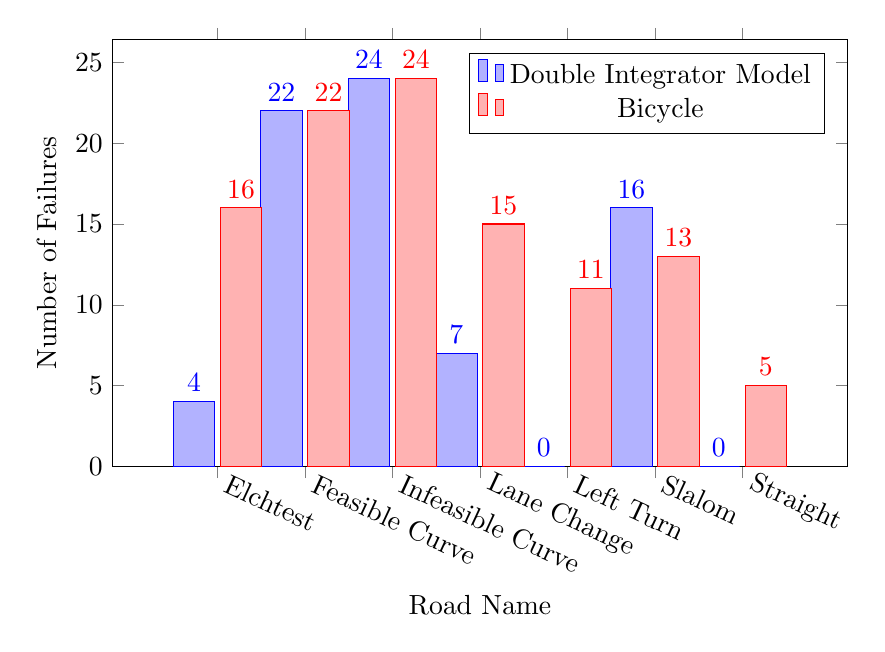
\begin{tikzpicture}
		\begin{axis}[
				ybar,
				bar width=15pt, % Increase bar width
				width=0.9\textwidth, % Increase overall figure width
				height=7cm,
				enlarge x limits=0.2, % Add some space on both sides
				symbolic x coords={Elchtest, Feasible Curve, Infeasible Curve, Lane Change, Left Turn, Slalom, Straight}, % Replace with actual road names
				xtick=data,
				xticklabel style={rotate=-25, anchor=west}, % Rotate labels for readability
				ymin=0,
				ylabel={Number of Failures},
				xlabel={Road Name},
				legend pos=north east,
				nodes near coords
			]
			% Replace the values below with actual failure counts
			\addplot coordinates {(Elchtest,4) (Feasible Curve,22) (Infeasible Curve,24) (Lane Change,7) (Left Turn,0) (Slalom,16) (Straight,0)};
			\addlegendentry{Double Integrator Model}

			\addplot coordinates {(Elchtest,16) (Feasible Curve,22) (Infeasible Curve,24) (Lane Change,15) (Left Turn,11) (Slalom,13) (Straight,5)};
			\addlegendentry{Bicycle}
		\end{axis}
	\end{tikzpicture}
	\caption{Histogram of Failed Scenarios per Model}
	\label{fig:failed_scenarios}
\end{figure}

The results indicate that higher speeds lead to higher failure rates.
However, an anomaly occurs in the Straight scenario, where the bicycle model has a higher failure rate at lower velocities.
This issue arises when using the $J_{\text{terminal}}$ objective function, which prioritizes velocity maximization.
This suggests a numerical instability that may be resolved using soft constraints.

\begin{figure}[h]
	\centering
	\begin{tikzpicture}
		\begin{groupplot}[
				group style={group size=2 by 1, horizontal sep=2cm}, % Two plots side by side
				width=0.5\textwidth, % Adjust width for each plot
				height=7cm,
				symbolic x coords={Elchtest, Feasible Curve, Lane Change, Left Turn, Slalom, Straight}, % Road names
				xtick=data,
				xticklabel style={rotate=-45, anchor=west}, % Rotate labels for readability
				ymin=0,
				ylabel={Number of Failures},
				xlabel={Road Name},
			]

			\nextgroupplot[
				title={Double Integrator Model},
				ybar stacked, % Stacked bars
				bar width=15pt, % Moved inside the groupplot
				nodes near coords, % Show numbers on bars
				every node near coord/.append style={yshift=-1pt}, % Move numbers slightly down
			]
			\addplot coordinates { (Elchtest, 0) (Feasible Curve, 6) (Lane Change, 0) (Left Turn, 0) (Slalom, 8) (Straight, 0) };
			\addplot coordinates { (Elchtest, 0) (Feasible Curve, 8) (Lane Change, 0) (Left Turn, 0) (Slalom, 0) (Straight, 0) };
			\addplot coordinates { (Elchtest, 4) (Feasible Curve, 8) (Lane Change, 7) (Left Turn, 0) (Slalom, 8) (Straight, 0) };
			\legend{5 m/s, 10 m/s, 20 m/s}

			% Second plot: Bicycle Model
			\nextgroupplot[
				title={Kinematic Bicycle Model},
				ybar stacked, % Stacked bars
				bar width=15pt, % Moved inside the groupplot
				nodes near coords, % Show numbers on bars
				every node near coord/.append style={yshift=-1pt}, % Move numbers slightly down
			]
			\addplot coordinates { (Elchtest, 3) (Feasible Curve, 6) (Lane Change, 3) (Left Turn, 2) (Slalom, 3) (Straight, 2) };
			\addplot coordinates { (Elchtest, 5) (Feasible Curve, 8) (Lane Change, 5) (Left Turn, 4) (Slalom, 5) (Straight, 2) };
			\addplot coordinates { (Elchtest, 8) (Feasible Curve, 8) (Lane Change, 7) (Left Turn, 5) (Slalom, 5) (Straight, 1) };
			\legend{5 m/s, 10 m/s, 20 m/s}
		\end{groupplot}
	\end{tikzpicture}
	\caption{Stacked Histogram of Failed Road Names per Model with Velocity}
	\label{fig:failed_scenarios_stacked}
\end{figure}

The bicycle model completes more runs in the slalom scenario compared to the double integrator model.
This is because the double integrator model considers the worst-case scenario and does not find a solution if it is infeasible to drive on the inner
side of the curve, even though it might be feasible to drive on the outer line.
For example driving at the highest speed $v_{max}$, the resulting polytope of the double integrator model is empty.
Limiting the vehicle options to the outer side and reduce the upper speed limit to $14.5$m/s results in a non-empty set.
In fact, we can observe that the bicycle model completes the slalom always at the outer lines (see \ref{fig:slalom_bicycle_model_n}), while driving
at around $14.5$m/s (see \ref{fig:slalom_bicycle_model_velocity}).

\begin{figure}[h!]
	\centering
	\resizebox{\textwidth}{!}{
		\begin{adjustbox}{clip, trim=0cm 14.5cm 0cm 4.8cm}
			%% Creator: Matplotlib, PGF backend
%%
%% To include the figure in your LaTeX document, write
%%   \input{<filename>.pgf}
%%
%% Make sure the required packages are loaded in your preamble
%%   \usepackage{pgf}
%%
%% Also ensure that all the required font packages are loaded; for instance,
%% the lmodern package is sometimes necessary when using math font.
%%   \usepackage{lmodern}
%%
%% Figures using additional raster images can only be included by \input if
%% they are in the same directory as the main LaTeX file. For loading figures
%% from other directories you can use the `import` package
%%   \usepackage{import}
%%
%% and then include the figures with
%%   \import{<path to file>}{<filename>.pgf}
%%
%% Matplotlib used the following preamble
%%   \def\mathdefault#1{#1}
%%   \everymath=\expandafter{\the\everymath\displaystyle}
%%   
%%   \ifdefined\pdftexversion\else  % non-pdftex case.
%%     \usepackage{fontspec}
%%   \fi
%%   \makeatletter\@ifpackageloaded{underscore}{}{\usepackage[strings]{underscore}}\makeatother
%%
\begingroup%
\makeatletter%
\begin{pgfpicture}%
\pgfpathrectangle{\pgfpointorigin}{\pgfqpoint{9.861316in}{7.457149in}}%
\pgfusepath{use as bounding box, clip}%
\begin{pgfscope}%
\pgfsetbuttcap%
\pgfsetmiterjoin%
\definecolor{currentfill}{rgb}{1.000000,1.000000,1.000000}%
\pgfsetfillcolor{currentfill}%
\pgfsetlinewidth{0.000000pt}%
\definecolor{currentstroke}{rgb}{1.000000,1.000000,1.000000}%
\pgfsetstrokecolor{currentstroke}%
\pgfsetdash{}{0pt}%
\pgfpathmoveto{\pgfqpoint{0.000000in}{0.000000in}}%
\pgfpathlineto{\pgfqpoint{9.861316in}{0.000000in}}%
\pgfpathlineto{\pgfqpoint{9.861316in}{7.457149in}}%
\pgfpathlineto{\pgfqpoint{0.000000in}{7.457149in}}%
\pgfpathlineto{\pgfqpoint{0.000000in}{0.000000in}}%
\pgfpathclose%
\pgfusepath{fill}%
\end{pgfscope}%
\begin{pgfscope}%
\pgfsetbuttcap%
\pgfsetmiterjoin%
\definecolor{currentfill}{rgb}{1.000000,1.000000,1.000000}%
\pgfsetfillcolor{currentfill}%
\pgfsetlinewidth{0.000000pt}%
\definecolor{currentstroke}{rgb}{0.000000,0.000000,0.000000}%
\pgfsetstrokecolor{currentstroke}%
\pgfsetstrokeopacity{0.000000}%
\pgfsetdash{}{0pt}%
\pgfpathmoveto{\pgfqpoint{0.716279in}{6.092222in}}%
\pgfpathlineto{\pgfqpoint{9.761316in}{6.092222in}}%
\pgfpathlineto{\pgfqpoint{9.761316in}{7.357149in}}%
\pgfpathlineto{\pgfqpoint{0.716279in}{7.357149in}}%
\pgfpathlineto{\pgfqpoint{0.716279in}{6.092222in}}%
\pgfpathclose%
\pgfusepath{fill}%
\end{pgfscope}%
\begin{pgfscope}%
\pgfsetbuttcap%
\pgfsetroundjoin%
\definecolor{currentfill}{rgb}{0.000000,0.000000,0.000000}%
\pgfsetfillcolor{currentfill}%
\pgfsetlinewidth{0.803000pt}%
\definecolor{currentstroke}{rgb}{0.000000,0.000000,0.000000}%
\pgfsetstrokecolor{currentstroke}%
\pgfsetdash{}{0pt}%
\pgfsys@defobject{currentmarker}{\pgfqpoint{0.000000in}{-0.048611in}}{\pgfqpoint{0.000000in}{0.000000in}}{%
\pgfpathmoveto{\pgfqpoint{0.000000in}{0.000000in}}%
\pgfpathlineto{\pgfqpoint{0.000000in}{-0.048611in}}%
\pgfusepath{stroke,fill}%
}%
\begin{pgfscope}%
\pgfsys@transformshift{1.127417in}{6.092222in}%
\pgfsys@useobject{currentmarker}{}%
\end{pgfscope}%
\end{pgfscope}%
\begin{pgfscope}%
\definecolor{textcolor}{rgb}{0.000000,0.000000,0.000000}%
\pgfsetstrokecolor{textcolor}%
\pgfsetfillcolor{textcolor}%
\pgftext[x=1.127417in,y=5.995000in,,top]{\color{textcolor}{\rmfamily\fontsize{9.000000}{10.800000}\selectfont\catcode`\^=\active\def^{\ifmmode\sp\else\^{}\fi}\catcode`\%=\active\def%{\%}$\mathdefault{0}$}}%
\end{pgfscope}%
\begin{pgfscope}%
\pgfsetbuttcap%
\pgfsetroundjoin%
\definecolor{currentfill}{rgb}{0.000000,0.000000,0.000000}%
\pgfsetfillcolor{currentfill}%
\pgfsetlinewidth{0.803000pt}%
\definecolor{currentstroke}{rgb}{0.000000,0.000000,0.000000}%
\pgfsetstrokecolor{currentstroke}%
\pgfsetdash{}{0pt}%
\pgfsys@defobject{currentmarker}{\pgfqpoint{0.000000in}{-0.048611in}}{\pgfqpoint{0.000000in}{0.000000in}}{%
\pgfpathmoveto{\pgfqpoint{0.000000in}{0.000000in}}%
\pgfpathlineto{\pgfqpoint{0.000000in}{-0.048611in}}%
\pgfusepath{stroke,fill}%
}%
\begin{pgfscope}%
\pgfsys@transformshift{2.739723in}{6.092222in}%
\pgfsys@useobject{currentmarker}{}%
\end{pgfscope}%
\end{pgfscope}%
\begin{pgfscope}%
\definecolor{textcolor}{rgb}{0.000000,0.000000,0.000000}%
\pgfsetstrokecolor{textcolor}%
\pgfsetfillcolor{textcolor}%
\pgftext[x=2.739723in,y=5.995000in,,top]{\color{textcolor}{\rmfamily\fontsize{9.000000}{10.800000}\selectfont\catcode`\^=\active\def^{\ifmmode\sp\else\^{}\fi}\catcode`\%=\active\def%{\%}$\mathdefault{1}$}}%
\end{pgfscope}%
\begin{pgfscope}%
\pgfsetbuttcap%
\pgfsetroundjoin%
\definecolor{currentfill}{rgb}{0.000000,0.000000,0.000000}%
\pgfsetfillcolor{currentfill}%
\pgfsetlinewidth{0.803000pt}%
\definecolor{currentstroke}{rgb}{0.000000,0.000000,0.000000}%
\pgfsetstrokecolor{currentstroke}%
\pgfsetdash{}{0pt}%
\pgfsys@defobject{currentmarker}{\pgfqpoint{0.000000in}{-0.048611in}}{\pgfqpoint{0.000000in}{0.000000in}}{%
\pgfpathmoveto{\pgfqpoint{0.000000in}{0.000000in}}%
\pgfpathlineto{\pgfqpoint{0.000000in}{-0.048611in}}%
\pgfusepath{stroke,fill}%
}%
\begin{pgfscope}%
\pgfsys@transformshift{4.352029in}{6.092222in}%
\pgfsys@useobject{currentmarker}{}%
\end{pgfscope}%
\end{pgfscope}%
\begin{pgfscope}%
\definecolor{textcolor}{rgb}{0.000000,0.000000,0.000000}%
\pgfsetstrokecolor{textcolor}%
\pgfsetfillcolor{textcolor}%
\pgftext[x=4.352029in,y=5.995000in,,top]{\color{textcolor}{\rmfamily\fontsize{9.000000}{10.800000}\selectfont\catcode`\^=\active\def^{\ifmmode\sp\else\^{}\fi}\catcode`\%=\active\def%{\%}$\mathdefault{2}$}}%
\end{pgfscope}%
\begin{pgfscope}%
\pgfsetbuttcap%
\pgfsetroundjoin%
\definecolor{currentfill}{rgb}{0.000000,0.000000,0.000000}%
\pgfsetfillcolor{currentfill}%
\pgfsetlinewidth{0.803000pt}%
\definecolor{currentstroke}{rgb}{0.000000,0.000000,0.000000}%
\pgfsetstrokecolor{currentstroke}%
\pgfsetdash{}{0pt}%
\pgfsys@defobject{currentmarker}{\pgfqpoint{0.000000in}{-0.048611in}}{\pgfqpoint{0.000000in}{0.000000in}}{%
\pgfpathmoveto{\pgfqpoint{0.000000in}{0.000000in}}%
\pgfpathlineto{\pgfqpoint{0.000000in}{-0.048611in}}%
\pgfusepath{stroke,fill}%
}%
\begin{pgfscope}%
\pgfsys@transformshift{5.964335in}{6.092222in}%
\pgfsys@useobject{currentmarker}{}%
\end{pgfscope}%
\end{pgfscope}%
\begin{pgfscope}%
\definecolor{textcolor}{rgb}{0.000000,0.000000,0.000000}%
\pgfsetstrokecolor{textcolor}%
\pgfsetfillcolor{textcolor}%
\pgftext[x=5.964335in,y=5.995000in,,top]{\color{textcolor}{\rmfamily\fontsize{9.000000}{10.800000}\selectfont\catcode`\^=\active\def^{\ifmmode\sp\else\^{}\fi}\catcode`\%=\active\def%{\%}$\mathdefault{3}$}}%
\end{pgfscope}%
\begin{pgfscope}%
\pgfsetbuttcap%
\pgfsetroundjoin%
\definecolor{currentfill}{rgb}{0.000000,0.000000,0.000000}%
\pgfsetfillcolor{currentfill}%
\pgfsetlinewidth{0.803000pt}%
\definecolor{currentstroke}{rgb}{0.000000,0.000000,0.000000}%
\pgfsetstrokecolor{currentstroke}%
\pgfsetdash{}{0pt}%
\pgfsys@defobject{currentmarker}{\pgfqpoint{0.000000in}{-0.048611in}}{\pgfqpoint{0.000000in}{0.000000in}}{%
\pgfpathmoveto{\pgfqpoint{0.000000in}{0.000000in}}%
\pgfpathlineto{\pgfqpoint{0.000000in}{-0.048611in}}%
\pgfusepath{stroke,fill}%
}%
\begin{pgfscope}%
\pgfsys@transformshift{7.576641in}{6.092222in}%
\pgfsys@useobject{currentmarker}{}%
\end{pgfscope}%
\end{pgfscope}%
\begin{pgfscope}%
\definecolor{textcolor}{rgb}{0.000000,0.000000,0.000000}%
\pgfsetstrokecolor{textcolor}%
\pgfsetfillcolor{textcolor}%
\pgftext[x=7.576641in,y=5.995000in,,top]{\color{textcolor}{\rmfamily\fontsize{9.000000}{10.800000}\selectfont\catcode`\^=\active\def^{\ifmmode\sp\else\^{}\fi}\catcode`\%=\active\def%{\%}$\mathdefault{4}$}}%
\end{pgfscope}%
\begin{pgfscope}%
\pgfsetbuttcap%
\pgfsetroundjoin%
\definecolor{currentfill}{rgb}{0.000000,0.000000,0.000000}%
\pgfsetfillcolor{currentfill}%
\pgfsetlinewidth{0.803000pt}%
\definecolor{currentstroke}{rgb}{0.000000,0.000000,0.000000}%
\pgfsetstrokecolor{currentstroke}%
\pgfsetdash{}{0pt}%
\pgfsys@defobject{currentmarker}{\pgfqpoint{0.000000in}{-0.048611in}}{\pgfqpoint{0.000000in}{0.000000in}}{%
\pgfpathmoveto{\pgfqpoint{0.000000in}{0.000000in}}%
\pgfpathlineto{\pgfqpoint{0.000000in}{-0.048611in}}%
\pgfusepath{stroke,fill}%
}%
\begin{pgfscope}%
\pgfsys@transformshift{9.188947in}{6.092222in}%
\pgfsys@useobject{currentmarker}{}%
\end{pgfscope}%
\end{pgfscope}%
\begin{pgfscope}%
\definecolor{textcolor}{rgb}{0.000000,0.000000,0.000000}%
\pgfsetstrokecolor{textcolor}%
\pgfsetfillcolor{textcolor}%
\pgftext[x=9.188947in,y=5.995000in,,top]{\color{textcolor}{\rmfamily\fontsize{9.000000}{10.800000}\selectfont\catcode`\^=\active\def^{\ifmmode\sp\else\^{}\fi}\catcode`\%=\active\def%{\%}$\mathdefault{5}$}}%
\end{pgfscope}%
\begin{pgfscope}%
\definecolor{textcolor}{rgb}{0.000000,0.000000,0.000000}%
\pgfsetstrokecolor{textcolor}%
\pgfsetfillcolor{textcolor}%
\pgftext[x=5.238797in,y=5.828333in,,top]{\color{textcolor}{\rmfamily\fontsize{11.000000}{13.200000}\selectfont\catcode`\^=\active\def^{\ifmmode\sp\else\^{}\fi}\catcode`\%=\active\def%{\%}Time [s]}}%
\end{pgfscope}%
\begin{pgfscope}%
\pgfsetbuttcap%
\pgfsetroundjoin%
\definecolor{currentfill}{rgb}{0.000000,0.000000,0.000000}%
\pgfsetfillcolor{currentfill}%
\pgfsetlinewidth{0.803000pt}%
\definecolor{currentstroke}{rgb}{0.000000,0.000000,0.000000}%
\pgfsetstrokecolor{currentstroke}%
\pgfsetdash{}{0pt}%
\pgfsys@defobject{currentmarker}{\pgfqpoint{-0.048611in}{0.000000in}}{\pgfqpoint{-0.000000in}{0.000000in}}{%
\pgfpathmoveto{\pgfqpoint{-0.000000in}{0.000000in}}%
\pgfpathlineto{\pgfqpoint{-0.048611in}{0.000000in}}%
\pgfusepath{stroke,fill}%
}%
\begin{pgfscope}%
\pgfsys@transformshift{0.716279in}{6.149719in}%
\pgfsys@useobject{currentmarker}{}%
\end{pgfscope}%
\end{pgfscope}%
\begin{pgfscope}%
\definecolor{textcolor}{rgb}{0.000000,0.000000,0.000000}%
\pgfsetstrokecolor{textcolor}%
\pgfsetfillcolor{textcolor}%
\pgftext[x=0.554821in, y=6.106316in, left, base]{\color{textcolor}{\rmfamily\fontsize{9.000000}{10.800000}\selectfont\catcode`\^=\active\def^{\ifmmode\sp\else\^{}\fi}\catcode`\%=\active\def%{\%}$\mathdefault{0}$}}%
\end{pgfscope}%
\begin{pgfscope}%
\pgfsetbuttcap%
\pgfsetroundjoin%
\definecolor{currentfill}{rgb}{0.000000,0.000000,0.000000}%
\pgfsetfillcolor{currentfill}%
\pgfsetlinewidth{0.803000pt}%
\definecolor{currentstroke}{rgb}{0.000000,0.000000,0.000000}%
\pgfsetstrokecolor{currentstroke}%
\pgfsetdash{}{0pt}%
\pgfsys@defobject{currentmarker}{\pgfqpoint{-0.048611in}{0.000000in}}{\pgfqpoint{-0.000000in}{0.000000in}}{%
\pgfpathmoveto{\pgfqpoint{-0.000000in}{0.000000in}}%
\pgfpathlineto{\pgfqpoint{-0.048611in}{0.000000in}}%
\pgfusepath{stroke,fill}%
}%
\begin{pgfscope}%
\pgfsys@transformshift{0.716279in}{6.494458in}%
\pgfsys@useobject{currentmarker}{}%
\end{pgfscope}%
\end{pgfscope}%
\begin{pgfscope}%
\definecolor{textcolor}{rgb}{0.000000,0.000000,0.000000}%
\pgfsetstrokecolor{textcolor}%
\pgfsetfillcolor{textcolor}%
\pgftext[x=0.490585in, y=6.451056in, left, base]{\color{textcolor}{\rmfamily\fontsize{9.000000}{10.800000}\selectfont\catcode`\^=\active\def^{\ifmmode\sp\else\^{}\fi}\catcode`\%=\active\def%{\%}$\mathdefault{10}$}}%
\end{pgfscope}%
\begin{pgfscope}%
\pgfsetbuttcap%
\pgfsetroundjoin%
\definecolor{currentfill}{rgb}{0.000000,0.000000,0.000000}%
\pgfsetfillcolor{currentfill}%
\pgfsetlinewidth{0.803000pt}%
\definecolor{currentstroke}{rgb}{0.000000,0.000000,0.000000}%
\pgfsetstrokecolor{currentstroke}%
\pgfsetdash{}{0pt}%
\pgfsys@defobject{currentmarker}{\pgfqpoint{-0.048611in}{0.000000in}}{\pgfqpoint{-0.000000in}{0.000000in}}{%
\pgfpathmoveto{\pgfqpoint{-0.000000in}{0.000000in}}%
\pgfpathlineto{\pgfqpoint{-0.048611in}{0.000000in}}%
\pgfusepath{stroke,fill}%
}%
\begin{pgfscope}%
\pgfsys@transformshift{0.716279in}{6.839198in}%
\pgfsys@useobject{currentmarker}{}%
\end{pgfscope}%
\end{pgfscope}%
\begin{pgfscope}%
\definecolor{textcolor}{rgb}{0.000000,0.000000,0.000000}%
\pgfsetstrokecolor{textcolor}%
\pgfsetfillcolor{textcolor}%
\pgftext[x=0.490585in, y=6.795795in, left, base]{\color{textcolor}{\rmfamily\fontsize{9.000000}{10.800000}\selectfont\catcode`\^=\active\def^{\ifmmode\sp\else\^{}\fi}\catcode`\%=\active\def%{\%}$\mathdefault{20}$}}%
\end{pgfscope}%
\begin{pgfscope}%
\pgfsetbuttcap%
\pgfsetroundjoin%
\definecolor{currentfill}{rgb}{0.000000,0.000000,0.000000}%
\pgfsetfillcolor{currentfill}%
\pgfsetlinewidth{0.803000pt}%
\definecolor{currentstroke}{rgb}{0.000000,0.000000,0.000000}%
\pgfsetstrokecolor{currentstroke}%
\pgfsetdash{}{0pt}%
\pgfsys@defobject{currentmarker}{\pgfqpoint{-0.048611in}{0.000000in}}{\pgfqpoint{-0.000000in}{0.000000in}}{%
\pgfpathmoveto{\pgfqpoint{-0.000000in}{0.000000in}}%
\pgfpathlineto{\pgfqpoint{-0.048611in}{0.000000in}}%
\pgfusepath{stroke,fill}%
}%
\begin{pgfscope}%
\pgfsys@transformshift{0.716279in}{7.183938in}%
\pgfsys@useobject{currentmarker}{}%
\end{pgfscope}%
\end{pgfscope}%
\begin{pgfscope}%
\definecolor{textcolor}{rgb}{0.000000,0.000000,0.000000}%
\pgfsetstrokecolor{textcolor}%
\pgfsetfillcolor{textcolor}%
\pgftext[x=0.490585in, y=7.140535in, left, base]{\color{textcolor}{\rmfamily\fontsize{9.000000}{10.800000}\selectfont\catcode`\^=\active\def^{\ifmmode\sp\else\^{}\fi}\catcode`\%=\active\def%{\%}$\mathdefault{30}$}}%
\end{pgfscope}%
\begin{pgfscope}%
\definecolor{textcolor}{rgb}{0.000000,0.000000,0.000000}%
\pgfsetstrokecolor{textcolor}%
\pgfsetfillcolor{textcolor}%
\pgftext[x=0.435029in,y=6.724686in,,bottom,rotate=90.000000]{\color{textcolor}{\rmfamily\fontsize{11.000000}{13.200000}\selectfont\catcode`\^=\active\def^{\ifmmode\sp\else\^{}\fi}\catcode`\%=\active\def%{\%}s}}%
\end{pgfscope}%
\begin{pgfscope}%
\pgfpathrectangle{\pgfqpoint{0.716279in}{6.092222in}}{\pgfqpoint{9.045038in}{1.264927in}}%
\pgfusepath{clip}%
\pgfsetrectcap%
\pgfsetroundjoin%
\pgfsetlinewidth{1.505625pt}%
\definecolor{currentstroke}{rgb}{0.000000,0.000000,1.000000}%
\pgfsetstrokecolor{currentstroke}%
\pgfsetdash{}{0pt}%
\pgfpathmoveto{\pgfqpoint{1.159663in}{6.153166in}}%
\pgfpathlineto{\pgfqpoint{1.353140in}{6.175147in}}%
\pgfpathlineto{\pgfqpoint{1.546616in}{6.199120in}}%
\pgfpathlineto{\pgfqpoint{1.740093in}{6.225072in}}%
\pgfpathlineto{\pgfqpoint{2.223785in}{6.293550in}}%
\pgfpathlineto{\pgfqpoint{2.481754in}{6.329857in}}%
\pgfpathlineto{\pgfqpoint{3.191169in}{6.430051in}}%
\pgfpathlineto{\pgfqpoint{3.449138in}{6.466355in}}%
\pgfpathlineto{\pgfqpoint{4.158552in}{6.566546in}}%
\pgfpathlineto{\pgfqpoint{4.416521in}{6.602849in}}%
\pgfpathlineto{\pgfqpoint{5.125936in}{6.703037in}}%
\pgfpathlineto{\pgfqpoint{5.383905in}{6.739338in}}%
\pgfpathlineto{\pgfqpoint{6.093320in}{6.839523in}}%
\pgfpathlineto{\pgfqpoint{6.351289in}{6.875822in}}%
\pgfpathlineto{\pgfqpoint{7.060703in}{6.976005in}}%
\pgfpathlineto{\pgfqpoint{7.318672in}{7.012303in}}%
\pgfpathlineto{\pgfqpoint{8.028087in}{7.112482in}}%
\pgfpathlineto{\pgfqpoint{8.286056in}{7.148780in}}%
\pgfpathlineto{\pgfqpoint{9.350178in}{7.299652in}}%
\pgfpathlineto{\pgfqpoint{9.350178in}{7.299652in}}%
\pgfusepath{stroke}%
\end{pgfscope}%
\begin{pgfscope}%
\pgfpathrectangle{\pgfqpoint{0.716279in}{6.092222in}}{\pgfqpoint{9.045038in}{1.264927in}}%
\pgfusepath{clip}%
\pgfsetrectcap%
\pgfsetroundjoin%
\pgfsetlinewidth{1.505625pt}%
\definecolor{currentstroke}{rgb}{1.000000,0.000000,0.000000}%
\pgfsetstrokecolor{currentstroke}%
\pgfsetdash{}{0pt}%
\pgfpathmoveto{\pgfqpoint{0.000000in}{0.000000in}}%
\pgfusepath{stroke}%
\end{pgfscope}%
\begin{pgfscope}%
\pgfpathrectangle{\pgfqpoint{0.716279in}{6.092222in}}{\pgfqpoint{9.045038in}{1.264927in}}%
\pgfusepath{clip}%
\pgfsetrectcap%
\pgfsetroundjoin%
\pgfsetlinewidth{1.505625pt}%
\definecolor{currentstroke}{rgb}{0.000000,0.501961,0.000000}%
\pgfsetstrokecolor{currentstroke}%
\pgfsetdash{}{0pt}%
\pgfpathmoveto{\pgfqpoint{1.127417in}{6.149719in}}%
\pgfusepath{stroke}%
\end{pgfscope}%
\begin{pgfscope}%
\pgfsetrectcap%
\pgfsetmiterjoin%
\pgfsetlinewidth{0.803000pt}%
\definecolor{currentstroke}{rgb}{0.000000,0.000000,0.000000}%
\pgfsetstrokecolor{currentstroke}%
\pgfsetdash{}{0pt}%
\pgfpathmoveto{\pgfqpoint{0.716279in}{6.092222in}}%
\pgfpathlineto{\pgfqpoint{0.716279in}{7.357149in}}%
\pgfusepath{stroke}%
\end{pgfscope}%
\begin{pgfscope}%
\pgfsetrectcap%
\pgfsetmiterjoin%
\pgfsetlinewidth{0.803000pt}%
\definecolor{currentstroke}{rgb}{0.000000,0.000000,0.000000}%
\pgfsetstrokecolor{currentstroke}%
\pgfsetdash{}{0pt}%
\pgfpathmoveto{\pgfqpoint{9.761316in}{6.092222in}}%
\pgfpathlineto{\pgfqpoint{9.761316in}{7.357149in}}%
\pgfusepath{stroke}%
\end{pgfscope}%
\begin{pgfscope}%
\pgfsetrectcap%
\pgfsetmiterjoin%
\pgfsetlinewidth{0.803000pt}%
\definecolor{currentstroke}{rgb}{0.000000,0.000000,0.000000}%
\pgfsetstrokecolor{currentstroke}%
\pgfsetdash{}{0pt}%
\pgfpathmoveto{\pgfqpoint{0.716279in}{6.092222in}}%
\pgfpathlineto{\pgfqpoint{9.761316in}{6.092222in}}%
\pgfusepath{stroke}%
\end{pgfscope}%
\begin{pgfscope}%
\pgfsetrectcap%
\pgfsetmiterjoin%
\pgfsetlinewidth{0.803000pt}%
\definecolor{currentstroke}{rgb}{0.000000,0.000000,0.000000}%
\pgfsetstrokecolor{currentstroke}%
\pgfsetdash{}{0pt}%
\pgfpathmoveto{\pgfqpoint{0.716279in}{7.357149in}}%
\pgfpathlineto{\pgfqpoint{9.761316in}{7.357149in}}%
\pgfusepath{stroke}%
\end{pgfscope}%
\begin{pgfscope}%
\pgfsetbuttcap%
\pgfsetmiterjoin%
\definecolor{currentfill}{rgb}{1.000000,1.000000,1.000000}%
\pgfsetfillcolor{currentfill}%
\pgfsetfillopacity{0.800000}%
\pgfsetlinewidth{1.003750pt}%
\definecolor{currentstroke}{rgb}{0.800000,0.800000,0.800000}%
\pgfsetstrokecolor{currentstroke}%
\pgfsetstrokeopacity{0.800000}%
\pgfsetdash{}{0pt}%
\pgfpathmoveto{\pgfqpoint{0.813501in}{6.665019in}}%
\pgfpathlineto{\pgfqpoint{1.481711in}{6.665019in}}%
\pgfpathquadraticcurveto{\pgfqpoint{1.509489in}{6.665019in}}{\pgfqpoint{1.509489in}{6.692797in}}%
\pgfpathlineto{\pgfqpoint{1.509489in}{7.259927in}}%
\pgfpathquadraticcurveto{\pgfqpoint{1.509489in}{7.287704in}}{\pgfqpoint{1.481711in}{7.287704in}}%
\pgfpathlineto{\pgfqpoint{0.813501in}{7.287704in}}%
\pgfpathquadraticcurveto{\pgfqpoint{0.785723in}{7.287704in}}{\pgfqpoint{0.785723in}{7.259927in}}%
\pgfpathlineto{\pgfqpoint{0.785723in}{6.692797in}}%
\pgfpathquadraticcurveto{\pgfqpoint{0.785723in}{6.665019in}}{\pgfqpoint{0.813501in}{6.665019in}}%
\pgfpathlineto{\pgfqpoint{0.813501in}{6.665019in}}%
\pgfpathclose%
\pgfusepath{stroke,fill}%
\end{pgfscope}%
\begin{pgfscope}%
\pgfsetrectcap%
\pgfsetroundjoin%
\pgfsetlinewidth{1.505625pt}%
\definecolor{currentstroke}{rgb}{0.000000,0.000000,1.000000}%
\pgfsetstrokecolor{currentstroke}%
\pgfsetdash{}{0pt}%
\pgfpathmoveto{\pgfqpoint{0.841279in}{7.183538in}}%
\pgfpathlineto{\pgfqpoint{0.980168in}{7.183538in}}%
\pgfpathlineto{\pgfqpoint{1.119056in}{7.183538in}}%
\pgfusepath{stroke}%
\end{pgfscope}%
\begin{pgfscope}%
\definecolor{textcolor}{rgb}{0.000000,0.000000,0.000000}%
\pgfsetstrokecolor{textcolor}%
\pgfsetfillcolor{textcolor}%
\pgftext[x=1.230168in,y=7.134927in,left,base]{\color{textcolor}{\rmfamily\fontsize{10.000000}{12.000000}\selectfont\catcode`\^=\active\def^{\ifmmode\sp\else\^{}\fi}\catcode`\%=\active\def%{\%}pos}}%
\end{pgfscope}%
\begin{pgfscope}%
\pgfsetrectcap%
\pgfsetroundjoin%
\pgfsetlinewidth{1.505625pt}%
\definecolor{currentstroke}{rgb}{1.000000,0.000000,0.000000}%
\pgfsetstrokecolor{currentstroke}%
\pgfsetdash{}{0pt}%
\pgfpathmoveto{\pgfqpoint{0.841279in}{6.989865in}}%
\pgfpathlineto{\pgfqpoint{0.980168in}{6.989865in}}%
\pgfpathlineto{\pgfqpoint{1.119056in}{6.989865in}}%
\pgfusepath{stroke}%
\end{pgfscope}%
\begin{pgfscope}%
\definecolor{textcolor}{rgb}{0.000000,0.000000,0.000000}%
\pgfsetstrokecolor{textcolor}%
\pgfsetfillcolor{textcolor}%
\pgftext[x=1.230168in,y=6.941254in,left,base]{\color{textcolor}{\rmfamily\fontsize{10.000000}{12.000000}\selectfont\catcode`\^=\active\def^{\ifmmode\sp\else\^{}\fi}\catcode`\%=\active\def%{\%}neg}}%
\end{pgfscope}%
\begin{pgfscope}%
\pgfsetrectcap%
\pgfsetroundjoin%
\pgfsetlinewidth{1.505625pt}%
\definecolor{currentstroke}{rgb}{0.000000,0.501961,0.000000}%
\pgfsetstrokecolor{currentstroke}%
\pgfsetdash{}{0pt}%
\pgfpathmoveto{\pgfqpoint{0.841279in}{6.796192in}}%
\pgfpathlineto{\pgfqpoint{0.980168in}{6.796192in}}%
\pgfpathlineto{\pgfqpoint{1.119056in}{6.796192in}}%
\pgfusepath{stroke}%
\end{pgfscope}%
\begin{pgfscope}%
\definecolor{textcolor}{rgb}{0.000000,0.000000,0.000000}%
\pgfsetstrokecolor{textcolor}%
\pgfsetfillcolor{textcolor}%
\pgftext[x=1.230168in,y=6.747581in,left,base]{\color{textcolor}{\rmfamily\fontsize{10.000000}{12.000000}\selectfont\catcode`\^=\active\def^{\ifmmode\sp\else\^{}\fi}\catcode`\%=\active\def%{\%}= 0}}%
\end{pgfscope}%
\begin{pgfscope}%
\pgfsetbuttcap%
\pgfsetmiterjoin%
\definecolor{currentfill}{rgb}{1.000000,1.000000,1.000000}%
\pgfsetfillcolor{currentfill}%
\pgfsetlinewidth{0.000000pt}%
\definecolor{currentstroke}{rgb}{0.000000,0.000000,0.000000}%
\pgfsetstrokecolor{currentstroke}%
\pgfsetstrokeopacity{0.000000}%
\pgfsetdash{}{0pt}%
\pgfpathmoveto{\pgfqpoint{0.716279in}{4.233472in}}%
\pgfpathlineto{\pgfqpoint{9.761316in}{4.233472in}}%
\pgfpathlineto{\pgfqpoint{9.761316in}{5.498399in}}%
\pgfpathlineto{\pgfqpoint{0.716279in}{5.498399in}}%
\pgfpathlineto{\pgfqpoint{0.716279in}{4.233472in}}%
\pgfpathclose%
\pgfusepath{fill}%
\end{pgfscope}%
\begin{pgfscope}%
\pgfsetbuttcap%
\pgfsetroundjoin%
\definecolor{currentfill}{rgb}{0.000000,0.000000,0.000000}%
\pgfsetfillcolor{currentfill}%
\pgfsetlinewidth{0.803000pt}%
\definecolor{currentstroke}{rgb}{0.000000,0.000000,0.000000}%
\pgfsetstrokecolor{currentstroke}%
\pgfsetdash{}{0pt}%
\pgfsys@defobject{currentmarker}{\pgfqpoint{0.000000in}{-0.048611in}}{\pgfqpoint{0.000000in}{0.000000in}}{%
\pgfpathmoveto{\pgfqpoint{0.000000in}{0.000000in}}%
\pgfpathlineto{\pgfqpoint{0.000000in}{-0.048611in}}%
\pgfusepath{stroke,fill}%
}%
\begin{pgfscope}%
\pgfsys@transformshift{1.127417in}{4.233472in}%
\pgfsys@useobject{currentmarker}{}%
\end{pgfscope}%
\end{pgfscope}%
\begin{pgfscope}%
\definecolor{textcolor}{rgb}{0.000000,0.000000,0.000000}%
\pgfsetstrokecolor{textcolor}%
\pgfsetfillcolor{textcolor}%
\pgftext[x=1.127417in,y=4.136250in,,top]{\color{textcolor}{\rmfamily\fontsize{9.000000}{10.800000}\selectfont\catcode`\^=\active\def^{\ifmmode\sp\else\^{}\fi}\catcode`\%=\active\def%{\%}$\mathdefault{0}$}}%
\end{pgfscope}%
\begin{pgfscope}%
\pgfsetbuttcap%
\pgfsetroundjoin%
\definecolor{currentfill}{rgb}{0.000000,0.000000,0.000000}%
\pgfsetfillcolor{currentfill}%
\pgfsetlinewidth{0.803000pt}%
\definecolor{currentstroke}{rgb}{0.000000,0.000000,0.000000}%
\pgfsetstrokecolor{currentstroke}%
\pgfsetdash{}{0pt}%
\pgfsys@defobject{currentmarker}{\pgfqpoint{0.000000in}{-0.048611in}}{\pgfqpoint{0.000000in}{0.000000in}}{%
\pgfpathmoveto{\pgfqpoint{0.000000in}{0.000000in}}%
\pgfpathlineto{\pgfqpoint{0.000000in}{-0.048611in}}%
\pgfusepath{stroke,fill}%
}%
\begin{pgfscope}%
\pgfsys@transformshift{2.739723in}{4.233472in}%
\pgfsys@useobject{currentmarker}{}%
\end{pgfscope}%
\end{pgfscope}%
\begin{pgfscope}%
\definecolor{textcolor}{rgb}{0.000000,0.000000,0.000000}%
\pgfsetstrokecolor{textcolor}%
\pgfsetfillcolor{textcolor}%
\pgftext[x=2.739723in,y=4.136250in,,top]{\color{textcolor}{\rmfamily\fontsize{9.000000}{10.800000}\selectfont\catcode`\^=\active\def^{\ifmmode\sp\else\^{}\fi}\catcode`\%=\active\def%{\%}$\mathdefault{1}$}}%
\end{pgfscope}%
\begin{pgfscope}%
\pgfsetbuttcap%
\pgfsetroundjoin%
\definecolor{currentfill}{rgb}{0.000000,0.000000,0.000000}%
\pgfsetfillcolor{currentfill}%
\pgfsetlinewidth{0.803000pt}%
\definecolor{currentstroke}{rgb}{0.000000,0.000000,0.000000}%
\pgfsetstrokecolor{currentstroke}%
\pgfsetdash{}{0pt}%
\pgfsys@defobject{currentmarker}{\pgfqpoint{0.000000in}{-0.048611in}}{\pgfqpoint{0.000000in}{0.000000in}}{%
\pgfpathmoveto{\pgfqpoint{0.000000in}{0.000000in}}%
\pgfpathlineto{\pgfqpoint{0.000000in}{-0.048611in}}%
\pgfusepath{stroke,fill}%
}%
\begin{pgfscope}%
\pgfsys@transformshift{4.352029in}{4.233472in}%
\pgfsys@useobject{currentmarker}{}%
\end{pgfscope}%
\end{pgfscope}%
\begin{pgfscope}%
\definecolor{textcolor}{rgb}{0.000000,0.000000,0.000000}%
\pgfsetstrokecolor{textcolor}%
\pgfsetfillcolor{textcolor}%
\pgftext[x=4.352029in,y=4.136250in,,top]{\color{textcolor}{\rmfamily\fontsize{9.000000}{10.800000}\selectfont\catcode`\^=\active\def^{\ifmmode\sp\else\^{}\fi}\catcode`\%=\active\def%{\%}$\mathdefault{2}$}}%
\end{pgfscope}%
\begin{pgfscope}%
\pgfsetbuttcap%
\pgfsetroundjoin%
\definecolor{currentfill}{rgb}{0.000000,0.000000,0.000000}%
\pgfsetfillcolor{currentfill}%
\pgfsetlinewidth{0.803000pt}%
\definecolor{currentstroke}{rgb}{0.000000,0.000000,0.000000}%
\pgfsetstrokecolor{currentstroke}%
\pgfsetdash{}{0pt}%
\pgfsys@defobject{currentmarker}{\pgfqpoint{0.000000in}{-0.048611in}}{\pgfqpoint{0.000000in}{0.000000in}}{%
\pgfpathmoveto{\pgfqpoint{0.000000in}{0.000000in}}%
\pgfpathlineto{\pgfqpoint{0.000000in}{-0.048611in}}%
\pgfusepath{stroke,fill}%
}%
\begin{pgfscope}%
\pgfsys@transformshift{5.964335in}{4.233472in}%
\pgfsys@useobject{currentmarker}{}%
\end{pgfscope}%
\end{pgfscope}%
\begin{pgfscope}%
\definecolor{textcolor}{rgb}{0.000000,0.000000,0.000000}%
\pgfsetstrokecolor{textcolor}%
\pgfsetfillcolor{textcolor}%
\pgftext[x=5.964335in,y=4.136250in,,top]{\color{textcolor}{\rmfamily\fontsize{9.000000}{10.800000}\selectfont\catcode`\^=\active\def^{\ifmmode\sp\else\^{}\fi}\catcode`\%=\active\def%{\%}$\mathdefault{3}$}}%
\end{pgfscope}%
\begin{pgfscope}%
\pgfsetbuttcap%
\pgfsetroundjoin%
\definecolor{currentfill}{rgb}{0.000000,0.000000,0.000000}%
\pgfsetfillcolor{currentfill}%
\pgfsetlinewidth{0.803000pt}%
\definecolor{currentstroke}{rgb}{0.000000,0.000000,0.000000}%
\pgfsetstrokecolor{currentstroke}%
\pgfsetdash{}{0pt}%
\pgfsys@defobject{currentmarker}{\pgfqpoint{0.000000in}{-0.048611in}}{\pgfqpoint{0.000000in}{0.000000in}}{%
\pgfpathmoveto{\pgfqpoint{0.000000in}{0.000000in}}%
\pgfpathlineto{\pgfqpoint{0.000000in}{-0.048611in}}%
\pgfusepath{stroke,fill}%
}%
\begin{pgfscope}%
\pgfsys@transformshift{7.576641in}{4.233472in}%
\pgfsys@useobject{currentmarker}{}%
\end{pgfscope}%
\end{pgfscope}%
\begin{pgfscope}%
\definecolor{textcolor}{rgb}{0.000000,0.000000,0.000000}%
\pgfsetstrokecolor{textcolor}%
\pgfsetfillcolor{textcolor}%
\pgftext[x=7.576641in,y=4.136250in,,top]{\color{textcolor}{\rmfamily\fontsize{9.000000}{10.800000}\selectfont\catcode`\^=\active\def^{\ifmmode\sp\else\^{}\fi}\catcode`\%=\active\def%{\%}$\mathdefault{4}$}}%
\end{pgfscope}%
\begin{pgfscope}%
\pgfsetbuttcap%
\pgfsetroundjoin%
\definecolor{currentfill}{rgb}{0.000000,0.000000,0.000000}%
\pgfsetfillcolor{currentfill}%
\pgfsetlinewidth{0.803000pt}%
\definecolor{currentstroke}{rgb}{0.000000,0.000000,0.000000}%
\pgfsetstrokecolor{currentstroke}%
\pgfsetdash{}{0pt}%
\pgfsys@defobject{currentmarker}{\pgfqpoint{0.000000in}{-0.048611in}}{\pgfqpoint{0.000000in}{0.000000in}}{%
\pgfpathmoveto{\pgfqpoint{0.000000in}{0.000000in}}%
\pgfpathlineto{\pgfqpoint{0.000000in}{-0.048611in}}%
\pgfusepath{stroke,fill}%
}%
\begin{pgfscope}%
\pgfsys@transformshift{9.188947in}{4.233472in}%
\pgfsys@useobject{currentmarker}{}%
\end{pgfscope}%
\end{pgfscope}%
\begin{pgfscope}%
\definecolor{textcolor}{rgb}{0.000000,0.000000,0.000000}%
\pgfsetstrokecolor{textcolor}%
\pgfsetfillcolor{textcolor}%
\pgftext[x=9.188947in,y=4.136250in,,top]{\color{textcolor}{\rmfamily\fontsize{9.000000}{10.800000}\selectfont\catcode`\^=\active\def^{\ifmmode\sp\else\^{}\fi}\catcode`\%=\active\def%{\%}$\mathdefault{5}$}}%
\end{pgfscope}%
\begin{pgfscope}%
\definecolor{textcolor}{rgb}{0.000000,0.000000,0.000000}%
\pgfsetstrokecolor{textcolor}%
\pgfsetfillcolor{textcolor}%
\pgftext[x=5.238797in,y=3.969583in,,top]{\color{textcolor}{\rmfamily\fontsize{11.000000}{13.200000}\selectfont\catcode`\^=\active\def^{\ifmmode\sp\else\^{}\fi}\catcode`\%=\active\def%{\%}Time [s]}}%
\end{pgfscope}%
\begin{pgfscope}%
\pgfsetbuttcap%
\pgfsetroundjoin%
\definecolor{currentfill}{rgb}{0.000000,0.000000,0.000000}%
\pgfsetfillcolor{currentfill}%
\pgfsetlinewidth{0.803000pt}%
\definecolor{currentstroke}{rgb}{0.000000,0.000000,0.000000}%
\pgfsetstrokecolor{currentstroke}%
\pgfsetdash{}{0pt}%
\pgfsys@defobject{currentmarker}{\pgfqpoint{-0.048611in}{0.000000in}}{\pgfqpoint{-0.000000in}{0.000000in}}{%
\pgfpathmoveto{\pgfqpoint{-0.000000in}{0.000000in}}%
\pgfpathlineto{\pgfqpoint{-0.048611in}{0.000000in}}%
\pgfusepath{stroke,fill}%
}%
\begin{pgfscope}%
\pgfsys@transformshift{0.716279in}{4.282131in}%
\pgfsys@useobject{currentmarker}{}%
\end{pgfscope}%
\end{pgfscope}%
\begin{pgfscope}%
\definecolor{textcolor}{rgb}{0.000000,0.000000,0.000000}%
\pgfsetstrokecolor{textcolor}%
\pgfsetfillcolor{textcolor}%
\pgftext[x=0.290741in, y=4.238728in, left, base]{\color{textcolor}{\rmfamily\fontsize{9.000000}{10.800000}\selectfont\catcode`\^=\active\def^{\ifmmode\sp\else\^{}\fi}\catcode`\%=\active\def%{\%}$\mathdefault{\ensuremath{-}0.05}$}}%
\end{pgfscope}%
\begin{pgfscope}%
\pgfsetbuttcap%
\pgfsetroundjoin%
\definecolor{currentfill}{rgb}{0.000000,0.000000,0.000000}%
\pgfsetfillcolor{currentfill}%
\pgfsetlinewidth{0.803000pt}%
\definecolor{currentstroke}{rgb}{0.000000,0.000000,0.000000}%
\pgfsetstrokecolor{currentstroke}%
\pgfsetdash{}{0pt}%
\pgfsys@defobject{currentmarker}{\pgfqpoint{-0.048611in}{0.000000in}}{\pgfqpoint{-0.000000in}{0.000000in}}{%
\pgfpathmoveto{\pgfqpoint{-0.000000in}{0.000000in}}%
\pgfpathlineto{\pgfqpoint{-0.048611in}{0.000000in}}%
\pgfusepath{stroke,fill}%
}%
\begin{pgfscope}%
\pgfsys@transformshift{0.716279in}{4.572500in}%
\pgfsys@useobject{currentmarker}{}%
\end{pgfscope}%
\end{pgfscope}%
\begin{pgfscope}%
\definecolor{textcolor}{rgb}{0.000000,0.000000,0.000000}%
\pgfsetstrokecolor{textcolor}%
\pgfsetfillcolor{textcolor}%
\pgftext[x=0.390663in, y=4.529097in, left, base]{\color{textcolor}{\rmfamily\fontsize{9.000000}{10.800000}\selectfont\catcode`\^=\active\def^{\ifmmode\sp\else\^{}\fi}\catcode`\%=\active\def%{\%}$\mathdefault{0.00}$}}%
\end{pgfscope}%
\begin{pgfscope}%
\pgfsetbuttcap%
\pgfsetroundjoin%
\definecolor{currentfill}{rgb}{0.000000,0.000000,0.000000}%
\pgfsetfillcolor{currentfill}%
\pgfsetlinewidth{0.803000pt}%
\definecolor{currentstroke}{rgb}{0.000000,0.000000,0.000000}%
\pgfsetstrokecolor{currentstroke}%
\pgfsetdash{}{0pt}%
\pgfsys@defobject{currentmarker}{\pgfqpoint{-0.048611in}{0.000000in}}{\pgfqpoint{-0.000000in}{0.000000in}}{%
\pgfpathmoveto{\pgfqpoint{-0.000000in}{0.000000in}}%
\pgfpathlineto{\pgfqpoint{-0.048611in}{0.000000in}}%
\pgfusepath{stroke,fill}%
}%
\begin{pgfscope}%
\pgfsys@transformshift{0.716279in}{4.862868in}%
\pgfsys@useobject{currentmarker}{}%
\end{pgfscope}%
\end{pgfscope}%
\begin{pgfscope}%
\definecolor{textcolor}{rgb}{0.000000,0.000000,0.000000}%
\pgfsetstrokecolor{textcolor}%
\pgfsetfillcolor{textcolor}%
\pgftext[x=0.390663in, y=4.819465in, left, base]{\color{textcolor}{\rmfamily\fontsize{9.000000}{10.800000}\selectfont\catcode`\^=\active\def^{\ifmmode\sp\else\^{}\fi}\catcode`\%=\active\def%{\%}$\mathdefault{0.05}$}}%
\end{pgfscope}%
\begin{pgfscope}%
\pgfsetbuttcap%
\pgfsetroundjoin%
\definecolor{currentfill}{rgb}{0.000000,0.000000,0.000000}%
\pgfsetfillcolor{currentfill}%
\pgfsetlinewidth{0.803000pt}%
\definecolor{currentstroke}{rgb}{0.000000,0.000000,0.000000}%
\pgfsetstrokecolor{currentstroke}%
\pgfsetdash{}{0pt}%
\pgfsys@defobject{currentmarker}{\pgfqpoint{-0.048611in}{0.000000in}}{\pgfqpoint{-0.000000in}{0.000000in}}{%
\pgfpathmoveto{\pgfqpoint{-0.000000in}{0.000000in}}%
\pgfpathlineto{\pgfqpoint{-0.048611in}{0.000000in}}%
\pgfusepath{stroke,fill}%
}%
\begin{pgfscope}%
\pgfsys@transformshift{0.716279in}{5.153236in}%
\pgfsys@useobject{currentmarker}{}%
\end{pgfscope}%
\end{pgfscope}%
\begin{pgfscope}%
\definecolor{textcolor}{rgb}{0.000000,0.000000,0.000000}%
\pgfsetstrokecolor{textcolor}%
\pgfsetfillcolor{textcolor}%
\pgftext[x=0.390663in, y=5.109834in, left, base]{\color{textcolor}{\rmfamily\fontsize{9.000000}{10.800000}\selectfont\catcode`\^=\active\def^{\ifmmode\sp\else\^{}\fi}\catcode`\%=\active\def%{\%}$\mathdefault{0.10}$}}%
\end{pgfscope}%
\begin{pgfscope}%
\pgfsetbuttcap%
\pgfsetroundjoin%
\definecolor{currentfill}{rgb}{0.000000,0.000000,0.000000}%
\pgfsetfillcolor{currentfill}%
\pgfsetlinewidth{0.803000pt}%
\definecolor{currentstroke}{rgb}{0.000000,0.000000,0.000000}%
\pgfsetstrokecolor{currentstroke}%
\pgfsetdash{}{0pt}%
\pgfsys@defobject{currentmarker}{\pgfqpoint{-0.048611in}{0.000000in}}{\pgfqpoint{-0.000000in}{0.000000in}}{%
\pgfpathmoveto{\pgfqpoint{-0.000000in}{0.000000in}}%
\pgfpathlineto{\pgfqpoint{-0.048611in}{0.000000in}}%
\pgfusepath{stroke,fill}%
}%
\begin{pgfscope}%
\pgfsys@transformshift{0.716279in}{5.443605in}%
\pgfsys@useobject{currentmarker}{}%
\end{pgfscope}%
\end{pgfscope}%
\begin{pgfscope}%
\definecolor{textcolor}{rgb}{0.000000,0.000000,0.000000}%
\pgfsetstrokecolor{textcolor}%
\pgfsetfillcolor{textcolor}%
\pgftext[x=0.390663in, y=5.400202in, left, base]{\color{textcolor}{\rmfamily\fontsize{9.000000}{10.800000}\selectfont\catcode`\^=\active\def^{\ifmmode\sp\else\^{}\fi}\catcode`\%=\active\def%{\%}$\mathdefault{0.15}$}}%
\end{pgfscope}%
\begin{pgfscope}%
\definecolor{textcolor}{rgb}{0.000000,0.000000,0.000000}%
\pgfsetstrokecolor{textcolor}%
\pgfsetfillcolor{textcolor}%
\pgftext[x=0.235185in,y=4.865936in,,bottom,rotate=90.000000]{\color{textcolor}{\rmfamily\fontsize{11.000000}{13.200000}\selectfont\catcode`\^=\active\def^{\ifmmode\sp\else\^{}\fi}\catcode`\%=\active\def%{\%}n}}%
\end{pgfscope}%
\begin{pgfscope}%
\pgfpathrectangle{\pgfqpoint{0.716279in}{4.233472in}}{\pgfqpoint{9.045038in}{1.264927in}}%
\pgfusepath{clip}%
\pgfsetrectcap%
\pgfsetroundjoin%
\pgfsetlinewidth{1.505625pt}%
\definecolor{currentstroke}{rgb}{0.000000,0.000000,1.000000}%
\pgfsetstrokecolor{currentstroke}%
\pgfsetdash{}{0pt}%
\pgfpathmoveto{\pgfqpoint{1.191909in}{4.576419in}}%
\pgfpathlineto{\pgfqpoint{1.224155in}{4.582773in}}%
\pgfpathlineto{\pgfqpoint{1.256401in}{4.590407in}}%
\pgfpathmoveto{\pgfqpoint{8.382794in}{4.574507in}}%
\pgfpathlineto{\pgfqpoint{8.415041in}{4.582901in}}%
\pgfpathlineto{\pgfqpoint{8.447287in}{4.595227in}}%
\pgfpathlineto{\pgfqpoint{8.479533in}{4.610322in}}%
\pgfpathlineto{\pgfqpoint{8.511779in}{4.627394in}}%
\pgfpathlineto{\pgfqpoint{8.544025in}{4.596868in}}%
\pgfpathlineto{\pgfqpoint{8.576271in}{4.602840in}}%
\pgfpathlineto{\pgfqpoint{8.608517in}{4.610748in}}%
\pgfpathlineto{\pgfqpoint{8.673010in}{4.629915in}}%
\pgfpathlineto{\pgfqpoint{8.705256in}{4.662220in}}%
\pgfpathlineto{\pgfqpoint{8.737502in}{4.660203in}}%
\pgfpathlineto{\pgfqpoint{8.769748in}{4.660445in}}%
\pgfpathlineto{\pgfqpoint{8.801994in}{4.662551in}}%
\pgfpathlineto{\pgfqpoint{8.834240in}{4.665843in}}%
\pgfpathlineto{\pgfqpoint{8.866486in}{4.846123in}}%
\pgfpathlineto{\pgfqpoint{8.898732in}{4.843081in}}%
\pgfpathlineto{\pgfqpoint{8.930978in}{4.842326in}}%
\pgfpathlineto{\pgfqpoint{8.963225in}{4.843412in}}%
\pgfpathlineto{\pgfqpoint{8.995471in}{4.845610in}}%
\pgfpathlineto{\pgfqpoint{9.027717in}{5.051814in}}%
\pgfpathlineto{\pgfqpoint{9.059963in}{5.048566in}}%
\pgfpathlineto{\pgfqpoint{9.092209in}{5.047625in}}%
\pgfpathlineto{\pgfqpoint{9.156701in}{5.050278in}}%
\pgfpathlineto{\pgfqpoint{9.188947in}{5.250879in}}%
\pgfpathlineto{\pgfqpoint{9.221194in}{5.247016in}}%
\pgfpathlineto{\pgfqpoint{9.253440in}{5.245278in}}%
\pgfpathlineto{\pgfqpoint{9.317932in}{5.245795in}}%
\pgfpathlineto{\pgfqpoint{9.350178in}{5.440902in}}%
\pgfpathlineto{\pgfqpoint{9.350178in}{5.440902in}}%
\pgfusepath{stroke}%
\end{pgfscope}%
\begin{pgfscope}%
\pgfpathrectangle{\pgfqpoint{0.716279in}{4.233472in}}{\pgfqpoint{9.045038in}{1.264927in}}%
\pgfusepath{clip}%
\pgfsetrectcap%
\pgfsetroundjoin%
\pgfsetlinewidth{1.505625pt}%
\definecolor{currentstroke}{rgb}{1.000000,0.000000,0.000000}%
\pgfsetstrokecolor{currentstroke}%
\pgfsetdash{}{0pt}%
\pgfpathmoveto{\pgfqpoint{1.288647in}{4.528431in}}%
\pgfpathlineto{\pgfqpoint{1.320893in}{4.526420in}}%
\pgfpathlineto{\pgfqpoint{1.353140in}{4.528503in}}%
\pgfpathlineto{\pgfqpoint{1.385386in}{4.533258in}}%
\pgfpathlineto{\pgfqpoint{1.417632in}{4.539481in}}%
\pgfpathlineto{\pgfqpoint{1.449878in}{4.444816in}}%
\pgfpathlineto{\pgfqpoint{1.482124in}{4.439606in}}%
\pgfpathlineto{\pgfqpoint{1.514370in}{4.438503in}}%
\pgfpathlineto{\pgfqpoint{1.546616in}{4.440328in}}%
\pgfpathlineto{\pgfqpoint{1.578862in}{4.443866in}}%
\pgfpathlineto{\pgfqpoint{1.611109in}{4.372210in}}%
\pgfpathlineto{\pgfqpoint{1.643355in}{4.364753in}}%
\pgfpathlineto{\pgfqpoint{1.675601in}{4.361517in}}%
\pgfpathlineto{\pgfqpoint{1.707847in}{4.361479in}}%
\pgfpathlineto{\pgfqpoint{1.740093in}{4.363400in}}%
\pgfpathlineto{\pgfqpoint{1.772339in}{4.322205in}}%
\pgfpathlineto{\pgfqpoint{1.836831in}{4.306528in}}%
\pgfpathlineto{\pgfqpoint{1.901324in}{4.294429in}}%
\pgfpathlineto{\pgfqpoint{1.933570in}{4.312159in}}%
\pgfpathlineto{\pgfqpoint{1.998062in}{4.300060in}}%
\pgfpathlineto{\pgfqpoint{2.062554in}{4.290969in}}%
\pgfpathlineto{\pgfqpoint{2.094800in}{4.330637in}}%
\pgfpathlineto{\pgfqpoint{2.159293in}{4.323349in}}%
\pgfpathlineto{\pgfqpoint{2.223785in}{4.318276in}}%
\pgfpathlineto{\pgfqpoint{2.256031in}{4.351548in}}%
\pgfpathlineto{\pgfqpoint{2.288277in}{4.349527in}}%
\pgfpathlineto{\pgfqpoint{2.320523in}{4.351658in}}%
\pgfpathlineto{\pgfqpoint{2.352769in}{4.356638in}}%
\pgfpathlineto{\pgfqpoint{2.385015in}{4.363257in}}%
\pgfpathlineto{\pgfqpoint{2.417262in}{4.346649in}}%
\pgfpathlineto{\pgfqpoint{2.449508in}{4.344579in}}%
\pgfpathlineto{\pgfqpoint{2.481754in}{4.346455in}}%
\pgfpathlineto{\pgfqpoint{2.514000in}{4.351054in}}%
\pgfpathlineto{\pgfqpoint{2.546246in}{4.357243in}}%
\pgfpathlineto{\pgfqpoint{2.578492in}{4.319179in}}%
\pgfpathlineto{\pgfqpoint{2.642984in}{4.313897in}}%
\pgfpathlineto{\pgfqpoint{2.707477in}{4.310761in}}%
\pgfpathlineto{\pgfqpoint{2.739723in}{4.313583in}}%
\pgfpathlineto{\pgfqpoint{2.804215in}{4.309624in}}%
\pgfpathlineto{\pgfqpoint{2.868707in}{4.307471in}}%
\pgfpathlineto{\pgfqpoint{2.900953in}{4.330497in}}%
\pgfpathlineto{\pgfqpoint{2.965446in}{4.329228in}}%
\pgfpathlineto{\pgfqpoint{3.029938in}{4.329322in}}%
\pgfpathlineto{\pgfqpoint{3.062184in}{4.349415in}}%
\pgfpathlineto{\pgfqpoint{3.094430in}{4.349684in}}%
\pgfpathlineto{\pgfqpoint{3.126676in}{4.354030in}}%
\pgfpathlineto{\pgfqpoint{3.158922in}{4.361029in}}%
\pgfpathlineto{\pgfqpoint{3.191169in}{4.369501in}}%
\pgfpathlineto{\pgfqpoint{3.223415in}{4.342163in}}%
\pgfpathlineto{\pgfqpoint{3.255661in}{4.341714in}}%
\pgfpathlineto{\pgfqpoint{3.287907in}{4.345333in}}%
\pgfpathlineto{\pgfqpoint{3.320153in}{4.351649in}}%
\pgfpathlineto{\pgfqpoint{3.352399in}{4.359481in}}%
\pgfpathlineto{\pgfqpoint{3.384645in}{4.309238in}}%
\pgfpathlineto{\pgfqpoint{3.449138in}{4.305734in}}%
\pgfpathlineto{\pgfqpoint{3.513630in}{4.303893in}}%
\pgfpathlineto{\pgfqpoint{3.545876in}{4.296729in}}%
\pgfpathlineto{\pgfqpoint{3.610368in}{4.293527in}}%
\pgfpathlineto{\pgfqpoint{3.674860in}{4.291999in}}%
\pgfpathlineto{\pgfqpoint{3.707107in}{4.309338in}}%
\pgfpathlineto{\pgfqpoint{3.771599in}{4.308329in}}%
\pgfpathlineto{\pgfqpoint{3.836091in}{4.308718in}}%
\pgfpathlineto{\pgfqpoint{3.868337in}{4.327219in}}%
\pgfpathlineto{\pgfqpoint{3.965076in}{4.328970in}}%
\pgfpathlineto{\pgfqpoint{3.997322in}{4.329976in}}%
\pgfpathlineto{\pgfqpoint{4.029568in}{4.343809in}}%
\pgfpathlineto{\pgfqpoint{4.061814in}{4.344830in}}%
\pgfpathlineto{\pgfqpoint{4.094060in}{4.349765in}}%
\pgfpathlineto{\pgfqpoint{4.126306in}{4.357210in}}%
\pgfpathlineto{\pgfqpoint{4.158552in}{4.366036in}}%
\pgfpathlineto{\pgfqpoint{4.190798in}{4.334843in}}%
\pgfpathlineto{\pgfqpoint{4.287537in}{4.335796in}}%
\pgfpathlineto{\pgfqpoint{4.319783in}{4.336542in}}%
\pgfpathlineto{\pgfqpoint{4.352029in}{4.324633in}}%
\pgfpathlineto{\pgfqpoint{4.448767in}{4.324814in}}%
\pgfpathlineto{\pgfqpoint{4.481013in}{4.325403in}}%
\pgfpathlineto{\pgfqpoint{4.513260in}{4.334853in}}%
\pgfpathlineto{\pgfqpoint{4.609998in}{4.336693in}}%
\pgfpathlineto{\pgfqpoint{4.642244in}{4.337701in}}%
\pgfpathlineto{\pgfqpoint{4.674490in}{4.348558in}}%
\pgfpathlineto{\pgfqpoint{4.706736in}{4.349501in}}%
\pgfpathlineto{\pgfqpoint{4.738982in}{4.354367in}}%
\pgfpathlineto{\pgfqpoint{4.771229in}{4.361753in}}%
\pgfpathlineto{\pgfqpoint{4.803475in}{4.370533in}}%
\pgfpathlineto{\pgfqpoint{4.835721in}{4.339133in}}%
\pgfpathlineto{\pgfqpoint{4.932459in}{4.339867in}}%
\pgfpathlineto{\pgfqpoint{4.964705in}{4.340525in}}%
\pgfpathlineto{\pgfqpoint{4.996951in}{4.328354in}}%
\pgfpathlineto{\pgfqpoint{5.093690in}{4.328184in}}%
\pgfpathlineto{\pgfqpoint{5.125936in}{4.328605in}}%
\pgfpathlineto{\pgfqpoint{5.158182in}{4.336717in}}%
\pgfpathlineto{\pgfqpoint{5.254920in}{4.338034in}}%
\pgfpathlineto{\pgfqpoint{5.287167in}{4.338847in}}%
\pgfpathlineto{\pgfqpoint{5.319413in}{4.348352in}}%
\pgfpathlineto{\pgfqpoint{5.351659in}{4.349074in}}%
\pgfpathlineto{\pgfqpoint{5.383905in}{4.353547in}}%
\pgfpathlineto{\pgfqpoint{5.416151in}{4.360429in}}%
\pgfpathlineto{\pgfqpoint{5.448397in}{4.368640in}}%
\pgfpathlineto{\pgfqpoint{5.480643in}{4.337960in}}%
\pgfpathlineto{\pgfqpoint{5.577382in}{4.338009in}}%
\pgfpathlineto{\pgfqpoint{5.609628in}{4.338392in}}%
\pgfpathlineto{\pgfqpoint{5.641874in}{4.325611in}}%
\pgfpathlineto{\pgfqpoint{5.738612in}{4.324644in}}%
\pgfpathlineto{\pgfqpoint{5.770858in}{4.324758in}}%
\pgfpathlineto{\pgfqpoint{5.803105in}{4.330942in}}%
\pgfpathlineto{\pgfqpoint{5.899843in}{4.331208in}}%
\pgfpathlineto{\pgfqpoint{5.932089in}{4.331649in}}%
\pgfpathlineto{\pgfqpoint{5.964335in}{4.339852in}}%
\pgfpathlineto{\pgfqpoint{5.996581in}{4.340194in}}%
\pgfpathlineto{\pgfqpoint{6.028827in}{4.344240in}}%
\pgfpathlineto{\pgfqpoint{6.061074in}{4.350687in}}%
\pgfpathlineto{\pgfqpoint{6.093320in}{4.358470in}}%
\pgfpathlineto{\pgfqpoint{6.125566in}{4.328804in}}%
\pgfpathlineto{\pgfqpoint{6.222304in}{4.328049in}}%
\pgfpathlineto{\pgfqpoint{6.254550in}{4.328228in}}%
\pgfpathlineto{\pgfqpoint{6.286796in}{4.317711in}}%
\pgfpathlineto{\pgfqpoint{6.383535in}{4.316341in}}%
\pgfpathlineto{\pgfqpoint{6.415781in}{4.316372in}}%
\pgfpathlineto{\pgfqpoint{6.448027in}{4.324889in}}%
\pgfpathlineto{\pgfqpoint{6.544765in}{4.325142in}}%
\pgfpathlineto{\pgfqpoint{6.577011in}{4.325635in}}%
\pgfpathlineto{\pgfqpoint{6.609258in}{4.336409in}}%
\pgfpathlineto{\pgfqpoint{6.738242in}{4.339230in}}%
\pgfpathlineto{\pgfqpoint{6.770488in}{4.348988in}}%
\pgfpathlineto{\pgfqpoint{6.802734in}{4.349932in}}%
\pgfpathlineto{\pgfqpoint{6.834980in}{4.354658in}}%
\pgfpathlineto{\pgfqpoint{6.867227in}{4.361800in}}%
\pgfpathlineto{\pgfqpoint{6.899473in}{4.370290in}}%
\pgfpathlineto{\pgfqpoint{6.931719in}{4.342218in}}%
\pgfpathlineto{\pgfqpoint{6.963965in}{4.342385in}}%
\pgfpathlineto{\pgfqpoint{6.996211in}{4.346059in}}%
\pgfpathlineto{\pgfqpoint{7.028457in}{4.352062in}}%
\pgfpathlineto{\pgfqpoint{7.060703in}{4.359433in}}%
\pgfpathlineto{\pgfqpoint{7.092949in}{4.322837in}}%
\pgfpathlineto{\pgfqpoint{7.157442in}{4.321709in}}%
\pgfpathlineto{\pgfqpoint{7.221934in}{4.322188in}}%
\pgfpathlineto{\pgfqpoint{7.254180in}{4.327476in}}%
\pgfpathlineto{\pgfqpoint{7.318672in}{4.327676in}}%
\pgfpathlineto{\pgfqpoint{7.383165in}{4.329527in}}%
\pgfpathlineto{\pgfqpoint{7.415411in}{4.356927in}}%
\pgfpathlineto{\pgfqpoint{7.447657in}{4.358349in}}%
\pgfpathlineto{\pgfqpoint{7.479903in}{4.363654in}}%
\pgfpathlineto{\pgfqpoint{7.512149in}{4.371527in}}%
\pgfpathlineto{\pgfqpoint{7.544395in}{4.380945in}}%
\pgfpathlineto{\pgfqpoint{7.576641in}{4.376264in}}%
\pgfpathlineto{\pgfqpoint{7.608887in}{4.378091in}}%
\pgfpathlineto{\pgfqpoint{7.641134in}{4.383568in}}%
\pgfpathlineto{\pgfqpoint{7.673380in}{4.391465in}}%
\pgfpathlineto{\pgfqpoint{7.705626in}{4.400840in}}%
\pgfpathlineto{\pgfqpoint{7.737872in}{4.384512in}}%
\pgfpathlineto{\pgfqpoint{7.770118in}{4.386300in}}%
\pgfpathlineto{\pgfqpoint{7.802364in}{4.392093in}}%
\pgfpathlineto{\pgfqpoint{7.834610in}{4.400597in}}%
\pgfpathlineto{\pgfqpoint{7.866856in}{4.410804in}}%
\pgfpathlineto{\pgfqpoint{7.899103in}{4.399916in}}%
\pgfpathlineto{\pgfqpoint{7.931349in}{4.402078in}}%
\pgfpathlineto{\pgfqpoint{7.963595in}{4.408331in}}%
\pgfpathlineto{\pgfqpoint{7.995841in}{4.417436in}}%
\pgfpathlineto{\pgfqpoint{8.028087in}{4.428415in}}%
\pgfpathlineto{\pgfqpoint{8.092579in}{4.434280in}}%
\pgfpathlineto{\pgfqpoint{8.124825in}{4.441453in}}%
\pgfpathlineto{\pgfqpoint{8.157072in}{4.451427in}}%
\pgfpathlineto{\pgfqpoint{8.189318in}{4.463347in}}%
\pgfpathlineto{\pgfqpoint{8.221564in}{4.489537in}}%
\pgfpathlineto{\pgfqpoint{8.253810in}{4.495044in}}%
\pgfpathlineto{\pgfqpoint{8.286056in}{4.504447in}}%
\pgfpathlineto{\pgfqpoint{8.318302in}{4.516609in}}%
\pgfpathlineto{\pgfqpoint{8.350548in}{4.530698in}}%
\pgfpathlineto{\pgfqpoint{8.350548in}{4.530698in}}%
\pgfusepath{stroke}%
\end{pgfscope}%
\begin{pgfscope}%
\pgfpathrectangle{\pgfqpoint{0.716279in}{4.233472in}}{\pgfqpoint{9.045038in}{1.264927in}}%
\pgfusepath{clip}%
\pgfsetrectcap%
\pgfsetroundjoin%
\pgfsetlinewidth{1.505625pt}%
\definecolor{currentstroke}{rgb}{0.000000,0.501961,0.000000}%
\pgfsetstrokecolor{currentstroke}%
\pgfsetdash{}{0pt}%
\pgfpathmoveto{\pgfqpoint{1.127417in}{4.572500in}}%
\pgfpathlineto{\pgfqpoint{1.159663in}{4.572500in}}%
\pgfpathlineto{\pgfqpoint{1.159663in}{4.572500in}}%
\pgfusepath{stroke}%
\end{pgfscope}%
\begin{pgfscope}%
\pgfsetrectcap%
\pgfsetmiterjoin%
\pgfsetlinewidth{0.803000pt}%
\definecolor{currentstroke}{rgb}{0.000000,0.000000,0.000000}%
\pgfsetstrokecolor{currentstroke}%
\pgfsetdash{}{0pt}%
\pgfpathmoveto{\pgfqpoint{0.716279in}{4.233472in}}%
\pgfpathlineto{\pgfqpoint{0.716279in}{5.498399in}}%
\pgfusepath{stroke}%
\end{pgfscope}%
\begin{pgfscope}%
\pgfsetrectcap%
\pgfsetmiterjoin%
\pgfsetlinewidth{0.803000pt}%
\definecolor{currentstroke}{rgb}{0.000000,0.000000,0.000000}%
\pgfsetstrokecolor{currentstroke}%
\pgfsetdash{}{0pt}%
\pgfpathmoveto{\pgfqpoint{9.761316in}{4.233472in}}%
\pgfpathlineto{\pgfqpoint{9.761316in}{5.498399in}}%
\pgfusepath{stroke}%
\end{pgfscope}%
\begin{pgfscope}%
\pgfsetrectcap%
\pgfsetmiterjoin%
\pgfsetlinewidth{0.803000pt}%
\definecolor{currentstroke}{rgb}{0.000000,0.000000,0.000000}%
\pgfsetstrokecolor{currentstroke}%
\pgfsetdash{}{0pt}%
\pgfpathmoveto{\pgfqpoint{0.716279in}{4.233472in}}%
\pgfpathlineto{\pgfqpoint{9.761316in}{4.233472in}}%
\pgfusepath{stroke}%
\end{pgfscope}%
\begin{pgfscope}%
\pgfsetrectcap%
\pgfsetmiterjoin%
\pgfsetlinewidth{0.803000pt}%
\definecolor{currentstroke}{rgb}{0.000000,0.000000,0.000000}%
\pgfsetstrokecolor{currentstroke}%
\pgfsetdash{}{0pt}%
\pgfpathmoveto{\pgfqpoint{0.716279in}{5.498399in}}%
\pgfpathlineto{\pgfqpoint{9.761316in}{5.498399in}}%
\pgfusepath{stroke}%
\end{pgfscope}%
\begin{pgfscope}%
\pgfsetbuttcap%
\pgfsetmiterjoin%
\definecolor{currentfill}{rgb}{1.000000,1.000000,1.000000}%
\pgfsetfillcolor{currentfill}%
\pgfsetfillopacity{0.800000}%
\pgfsetlinewidth{1.003750pt}%
\definecolor{currentstroke}{rgb}{0.800000,0.800000,0.800000}%
\pgfsetstrokecolor{currentstroke}%
\pgfsetstrokeopacity{0.800000}%
\pgfsetdash{}{0pt}%
\pgfpathmoveto{\pgfqpoint{0.813501in}{4.806269in}}%
\pgfpathlineto{\pgfqpoint{1.481711in}{4.806269in}}%
\pgfpathquadraticcurveto{\pgfqpoint{1.509489in}{4.806269in}}{\pgfqpoint{1.509489in}{4.834047in}}%
\pgfpathlineto{\pgfqpoint{1.509489in}{5.401177in}}%
\pgfpathquadraticcurveto{\pgfqpoint{1.509489in}{5.428954in}}{\pgfqpoint{1.481711in}{5.428954in}}%
\pgfpathlineto{\pgfqpoint{0.813501in}{5.428954in}}%
\pgfpathquadraticcurveto{\pgfqpoint{0.785723in}{5.428954in}}{\pgfqpoint{0.785723in}{5.401177in}}%
\pgfpathlineto{\pgfqpoint{0.785723in}{4.834047in}}%
\pgfpathquadraticcurveto{\pgfqpoint{0.785723in}{4.806269in}}{\pgfqpoint{0.813501in}{4.806269in}}%
\pgfpathlineto{\pgfqpoint{0.813501in}{4.806269in}}%
\pgfpathclose%
\pgfusepath{stroke,fill}%
\end{pgfscope}%
\begin{pgfscope}%
\pgfsetrectcap%
\pgfsetroundjoin%
\pgfsetlinewidth{1.505625pt}%
\definecolor{currentstroke}{rgb}{0.000000,0.000000,1.000000}%
\pgfsetstrokecolor{currentstroke}%
\pgfsetdash{}{0pt}%
\pgfpathmoveto{\pgfqpoint{0.841279in}{5.324788in}}%
\pgfpathlineto{\pgfqpoint{0.980168in}{5.324788in}}%
\pgfpathlineto{\pgfqpoint{1.119056in}{5.324788in}}%
\pgfusepath{stroke}%
\end{pgfscope}%
\begin{pgfscope}%
\definecolor{textcolor}{rgb}{0.000000,0.000000,0.000000}%
\pgfsetstrokecolor{textcolor}%
\pgfsetfillcolor{textcolor}%
\pgftext[x=1.230168in,y=5.276177in,left,base]{\color{textcolor}{\rmfamily\fontsize{10.000000}{12.000000}\selectfont\catcode`\^=\active\def^{\ifmmode\sp\else\^{}\fi}\catcode`\%=\active\def%{\%}pos}}%
\end{pgfscope}%
\begin{pgfscope}%
\pgfsetrectcap%
\pgfsetroundjoin%
\pgfsetlinewidth{1.505625pt}%
\definecolor{currentstroke}{rgb}{1.000000,0.000000,0.000000}%
\pgfsetstrokecolor{currentstroke}%
\pgfsetdash{}{0pt}%
\pgfpathmoveto{\pgfqpoint{0.841279in}{5.131115in}}%
\pgfpathlineto{\pgfqpoint{0.980168in}{5.131115in}}%
\pgfpathlineto{\pgfqpoint{1.119056in}{5.131115in}}%
\pgfusepath{stroke}%
\end{pgfscope}%
\begin{pgfscope}%
\definecolor{textcolor}{rgb}{0.000000,0.000000,0.000000}%
\pgfsetstrokecolor{textcolor}%
\pgfsetfillcolor{textcolor}%
\pgftext[x=1.230168in,y=5.082504in,left,base]{\color{textcolor}{\rmfamily\fontsize{10.000000}{12.000000}\selectfont\catcode`\^=\active\def^{\ifmmode\sp\else\^{}\fi}\catcode`\%=\active\def%{\%}neg}}%
\end{pgfscope}%
\begin{pgfscope}%
\pgfsetrectcap%
\pgfsetroundjoin%
\pgfsetlinewidth{1.505625pt}%
\definecolor{currentstroke}{rgb}{0.000000,0.501961,0.000000}%
\pgfsetstrokecolor{currentstroke}%
\pgfsetdash{}{0pt}%
\pgfpathmoveto{\pgfqpoint{0.841279in}{4.937442in}}%
\pgfpathlineto{\pgfqpoint{0.980168in}{4.937442in}}%
\pgfpathlineto{\pgfqpoint{1.119056in}{4.937442in}}%
\pgfusepath{stroke}%
\end{pgfscope}%
\begin{pgfscope}%
\definecolor{textcolor}{rgb}{0.000000,0.000000,0.000000}%
\pgfsetstrokecolor{textcolor}%
\pgfsetfillcolor{textcolor}%
\pgftext[x=1.230168in,y=4.888831in,left,base]{\color{textcolor}{\rmfamily\fontsize{10.000000}{12.000000}\selectfont\catcode`\^=\active\def^{\ifmmode\sp\else\^{}\fi}\catcode`\%=\active\def%{\%}= 0}}%
\end{pgfscope}%
\begin{pgfscope}%
\pgfsetbuttcap%
\pgfsetmiterjoin%
\definecolor{currentfill}{rgb}{1.000000,1.000000,1.000000}%
\pgfsetfillcolor{currentfill}%
\pgfsetlinewidth{0.000000pt}%
\definecolor{currentstroke}{rgb}{0.000000,0.000000,0.000000}%
\pgfsetstrokecolor{currentstroke}%
\pgfsetstrokeopacity{0.000000}%
\pgfsetdash{}{0pt}%
\pgfpathmoveto{\pgfqpoint{0.716279in}{2.374722in}}%
\pgfpathlineto{\pgfqpoint{9.761316in}{2.374722in}}%
\pgfpathlineto{\pgfqpoint{9.761316in}{3.639649in}}%
\pgfpathlineto{\pgfqpoint{0.716279in}{3.639649in}}%
\pgfpathlineto{\pgfqpoint{0.716279in}{2.374722in}}%
\pgfpathclose%
\pgfusepath{fill}%
\end{pgfscope}%
\begin{pgfscope}%
\pgfsetbuttcap%
\pgfsetroundjoin%
\definecolor{currentfill}{rgb}{0.000000,0.000000,0.000000}%
\pgfsetfillcolor{currentfill}%
\pgfsetlinewidth{0.803000pt}%
\definecolor{currentstroke}{rgb}{0.000000,0.000000,0.000000}%
\pgfsetstrokecolor{currentstroke}%
\pgfsetdash{}{0pt}%
\pgfsys@defobject{currentmarker}{\pgfqpoint{0.000000in}{-0.048611in}}{\pgfqpoint{0.000000in}{0.000000in}}{%
\pgfpathmoveto{\pgfqpoint{0.000000in}{0.000000in}}%
\pgfpathlineto{\pgfqpoint{0.000000in}{-0.048611in}}%
\pgfusepath{stroke,fill}%
}%
\begin{pgfscope}%
\pgfsys@transformshift{1.127417in}{2.374722in}%
\pgfsys@useobject{currentmarker}{}%
\end{pgfscope}%
\end{pgfscope}%
\begin{pgfscope}%
\definecolor{textcolor}{rgb}{0.000000,0.000000,0.000000}%
\pgfsetstrokecolor{textcolor}%
\pgfsetfillcolor{textcolor}%
\pgftext[x=1.127417in,y=2.277500in,,top]{\color{textcolor}{\rmfamily\fontsize{9.000000}{10.800000}\selectfont\catcode`\^=\active\def^{\ifmmode\sp\else\^{}\fi}\catcode`\%=\active\def%{\%}$\mathdefault{0}$}}%
\end{pgfscope}%
\begin{pgfscope}%
\pgfsetbuttcap%
\pgfsetroundjoin%
\definecolor{currentfill}{rgb}{0.000000,0.000000,0.000000}%
\pgfsetfillcolor{currentfill}%
\pgfsetlinewidth{0.803000pt}%
\definecolor{currentstroke}{rgb}{0.000000,0.000000,0.000000}%
\pgfsetstrokecolor{currentstroke}%
\pgfsetdash{}{0pt}%
\pgfsys@defobject{currentmarker}{\pgfqpoint{0.000000in}{-0.048611in}}{\pgfqpoint{0.000000in}{0.000000in}}{%
\pgfpathmoveto{\pgfqpoint{0.000000in}{0.000000in}}%
\pgfpathlineto{\pgfqpoint{0.000000in}{-0.048611in}}%
\pgfusepath{stroke,fill}%
}%
\begin{pgfscope}%
\pgfsys@transformshift{2.739723in}{2.374722in}%
\pgfsys@useobject{currentmarker}{}%
\end{pgfscope}%
\end{pgfscope}%
\begin{pgfscope}%
\definecolor{textcolor}{rgb}{0.000000,0.000000,0.000000}%
\pgfsetstrokecolor{textcolor}%
\pgfsetfillcolor{textcolor}%
\pgftext[x=2.739723in,y=2.277500in,,top]{\color{textcolor}{\rmfamily\fontsize{9.000000}{10.800000}\selectfont\catcode`\^=\active\def^{\ifmmode\sp\else\^{}\fi}\catcode`\%=\active\def%{\%}$\mathdefault{1}$}}%
\end{pgfscope}%
\begin{pgfscope}%
\pgfsetbuttcap%
\pgfsetroundjoin%
\definecolor{currentfill}{rgb}{0.000000,0.000000,0.000000}%
\pgfsetfillcolor{currentfill}%
\pgfsetlinewidth{0.803000pt}%
\definecolor{currentstroke}{rgb}{0.000000,0.000000,0.000000}%
\pgfsetstrokecolor{currentstroke}%
\pgfsetdash{}{0pt}%
\pgfsys@defobject{currentmarker}{\pgfqpoint{0.000000in}{-0.048611in}}{\pgfqpoint{0.000000in}{0.000000in}}{%
\pgfpathmoveto{\pgfqpoint{0.000000in}{0.000000in}}%
\pgfpathlineto{\pgfqpoint{0.000000in}{-0.048611in}}%
\pgfusepath{stroke,fill}%
}%
\begin{pgfscope}%
\pgfsys@transformshift{4.352029in}{2.374722in}%
\pgfsys@useobject{currentmarker}{}%
\end{pgfscope}%
\end{pgfscope}%
\begin{pgfscope}%
\definecolor{textcolor}{rgb}{0.000000,0.000000,0.000000}%
\pgfsetstrokecolor{textcolor}%
\pgfsetfillcolor{textcolor}%
\pgftext[x=4.352029in,y=2.277500in,,top]{\color{textcolor}{\rmfamily\fontsize{9.000000}{10.800000}\selectfont\catcode`\^=\active\def^{\ifmmode\sp\else\^{}\fi}\catcode`\%=\active\def%{\%}$\mathdefault{2}$}}%
\end{pgfscope}%
\begin{pgfscope}%
\pgfsetbuttcap%
\pgfsetroundjoin%
\definecolor{currentfill}{rgb}{0.000000,0.000000,0.000000}%
\pgfsetfillcolor{currentfill}%
\pgfsetlinewidth{0.803000pt}%
\definecolor{currentstroke}{rgb}{0.000000,0.000000,0.000000}%
\pgfsetstrokecolor{currentstroke}%
\pgfsetdash{}{0pt}%
\pgfsys@defobject{currentmarker}{\pgfqpoint{0.000000in}{-0.048611in}}{\pgfqpoint{0.000000in}{0.000000in}}{%
\pgfpathmoveto{\pgfqpoint{0.000000in}{0.000000in}}%
\pgfpathlineto{\pgfqpoint{0.000000in}{-0.048611in}}%
\pgfusepath{stroke,fill}%
}%
\begin{pgfscope}%
\pgfsys@transformshift{5.964335in}{2.374722in}%
\pgfsys@useobject{currentmarker}{}%
\end{pgfscope}%
\end{pgfscope}%
\begin{pgfscope}%
\definecolor{textcolor}{rgb}{0.000000,0.000000,0.000000}%
\pgfsetstrokecolor{textcolor}%
\pgfsetfillcolor{textcolor}%
\pgftext[x=5.964335in,y=2.277500in,,top]{\color{textcolor}{\rmfamily\fontsize{9.000000}{10.800000}\selectfont\catcode`\^=\active\def^{\ifmmode\sp\else\^{}\fi}\catcode`\%=\active\def%{\%}$\mathdefault{3}$}}%
\end{pgfscope}%
\begin{pgfscope}%
\pgfsetbuttcap%
\pgfsetroundjoin%
\definecolor{currentfill}{rgb}{0.000000,0.000000,0.000000}%
\pgfsetfillcolor{currentfill}%
\pgfsetlinewidth{0.803000pt}%
\definecolor{currentstroke}{rgb}{0.000000,0.000000,0.000000}%
\pgfsetstrokecolor{currentstroke}%
\pgfsetdash{}{0pt}%
\pgfsys@defobject{currentmarker}{\pgfqpoint{0.000000in}{-0.048611in}}{\pgfqpoint{0.000000in}{0.000000in}}{%
\pgfpathmoveto{\pgfqpoint{0.000000in}{0.000000in}}%
\pgfpathlineto{\pgfqpoint{0.000000in}{-0.048611in}}%
\pgfusepath{stroke,fill}%
}%
\begin{pgfscope}%
\pgfsys@transformshift{7.576641in}{2.374722in}%
\pgfsys@useobject{currentmarker}{}%
\end{pgfscope}%
\end{pgfscope}%
\begin{pgfscope}%
\definecolor{textcolor}{rgb}{0.000000,0.000000,0.000000}%
\pgfsetstrokecolor{textcolor}%
\pgfsetfillcolor{textcolor}%
\pgftext[x=7.576641in,y=2.277500in,,top]{\color{textcolor}{\rmfamily\fontsize{9.000000}{10.800000}\selectfont\catcode`\^=\active\def^{\ifmmode\sp\else\^{}\fi}\catcode`\%=\active\def%{\%}$\mathdefault{4}$}}%
\end{pgfscope}%
\begin{pgfscope}%
\pgfsetbuttcap%
\pgfsetroundjoin%
\definecolor{currentfill}{rgb}{0.000000,0.000000,0.000000}%
\pgfsetfillcolor{currentfill}%
\pgfsetlinewidth{0.803000pt}%
\definecolor{currentstroke}{rgb}{0.000000,0.000000,0.000000}%
\pgfsetstrokecolor{currentstroke}%
\pgfsetdash{}{0pt}%
\pgfsys@defobject{currentmarker}{\pgfqpoint{0.000000in}{-0.048611in}}{\pgfqpoint{0.000000in}{0.000000in}}{%
\pgfpathmoveto{\pgfqpoint{0.000000in}{0.000000in}}%
\pgfpathlineto{\pgfqpoint{0.000000in}{-0.048611in}}%
\pgfusepath{stroke,fill}%
}%
\begin{pgfscope}%
\pgfsys@transformshift{9.188947in}{2.374722in}%
\pgfsys@useobject{currentmarker}{}%
\end{pgfscope}%
\end{pgfscope}%
\begin{pgfscope}%
\definecolor{textcolor}{rgb}{0.000000,0.000000,0.000000}%
\pgfsetstrokecolor{textcolor}%
\pgfsetfillcolor{textcolor}%
\pgftext[x=9.188947in,y=2.277500in,,top]{\color{textcolor}{\rmfamily\fontsize{9.000000}{10.800000}\selectfont\catcode`\^=\active\def^{\ifmmode\sp\else\^{}\fi}\catcode`\%=\active\def%{\%}$\mathdefault{5}$}}%
\end{pgfscope}%
\begin{pgfscope}%
\definecolor{textcolor}{rgb}{0.000000,0.000000,0.000000}%
\pgfsetstrokecolor{textcolor}%
\pgfsetfillcolor{textcolor}%
\pgftext[x=5.238797in,y=2.110833in,,top]{\color{textcolor}{\rmfamily\fontsize{11.000000}{13.200000}\selectfont\catcode`\^=\active\def^{\ifmmode\sp\else\^{}\fi}\catcode`\%=\active\def%{\%}Time [s]}}%
\end{pgfscope}%
\begin{pgfscope}%
\pgfsetbuttcap%
\pgfsetroundjoin%
\definecolor{currentfill}{rgb}{0.000000,0.000000,0.000000}%
\pgfsetfillcolor{currentfill}%
\pgfsetlinewidth{0.803000pt}%
\definecolor{currentstroke}{rgb}{0.000000,0.000000,0.000000}%
\pgfsetstrokecolor{currentstroke}%
\pgfsetdash{}{0pt}%
\pgfsys@defobject{currentmarker}{\pgfqpoint{-0.048611in}{0.000000in}}{\pgfqpoint{-0.000000in}{0.000000in}}{%
\pgfpathmoveto{\pgfqpoint{-0.000000in}{0.000000in}}%
\pgfpathlineto{\pgfqpoint{-0.048611in}{0.000000in}}%
\pgfusepath{stroke,fill}%
}%
\begin{pgfscope}%
\pgfsys@transformshift{0.716279in}{2.432219in}%
\pgfsys@useobject{currentmarker}{}%
\end{pgfscope}%
\end{pgfscope}%
\begin{pgfscope}%
\definecolor{textcolor}{rgb}{0.000000,0.000000,0.000000}%
\pgfsetstrokecolor{textcolor}%
\pgfsetfillcolor{textcolor}%
\pgftext[x=0.454898in, y=2.388816in, left, base]{\color{textcolor}{\rmfamily\fontsize{9.000000}{10.800000}\selectfont\catcode`\^=\active\def^{\ifmmode\sp\else\^{}\fi}\catcode`\%=\active\def%{\%}$\mathdefault{5.0}$}}%
\end{pgfscope}%
\begin{pgfscope}%
\pgfsetbuttcap%
\pgfsetroundjoin%
\definecolor{currentfill}{rgb}{0.000000,0.000000,0.000000}%
\pgfsetfillcolor{currentfill}%
\pgfsetlinewidth{0.803000pt}%
\definecolor{currentstroke}{rgb}{0.000000,0.000000,0.000000}%
\pgfsetstrokecolor{currentstroke}%
\pgfsetdash{}{0pt}%
\pgfsys@defobject{currentmarker}{\pgfqpoint{-0.048611in}{0.000000in}}{\pgfqpoint{-0.000000in}{0.000000in}}{%
\pgfpathmoveto{\pgfqpoint{-0.000000in}{0.000000in}}%
\pgfpathlineto{\pgfqpoint{-0.048611in}{0.000000in}}%
\pgfusepath{stroke,fill}%
}%
\begin{pgfscope}%
\pgfsys@transformshift{0.716279in}{2.776555in}%
\pgfsys@useobject{currentmarker}{}%
\end{pgfscope}%
\end{pgfscope}%
\begin{pgfscope}%
\definecolor{textcolor}{rgb}{0.000000,0.000000,0.000000}%
\pgfsetstrokecolor{textcolor}%
\pgfsetfillcolor{textcolor}%
\pgftext[x=0.454898in, y=2.733152in, left, base]{\color{textcolor}{\rmfamily\fontsize{9.000000}{10.800000}\selectfont\catcode`\^=\active\def^{\ifmmode\sp\else\^{}\fi}\catcode`\%=\active\def%{\%}$\mathdefault{5.5}$}}%
\end{pgfscope}%
\begin{pgfscope}%
\pgfsetbuttcap%
\pgfsetroundjoin%
\definecolor{currentfill}{rgb}{0.000000,0.000000,0.000000}%
\pgfsetfillcolor{currentfill}%
\pgfsetlinewidth{0.803000pt}%
\definecolor{currentstroke}{rgb}{0.000000,0.000000,0.000000}%
\pgfsetstrokecolor{currentstroke}%
\pgfsetdash{}{0pt}%
\pgfsys@defobject{currentmarker}{\pgfqpoint{-0.048611in}{0.000000in}}{\pgfqpoint{-0.000000in}{0.000000in}}{%
\pgfpathmoveto{\pgfqpoint{-0.000000in}{0.000000in}}%
\pgfpathlineto{\pgfqpoint{-0.048611in}{0.000000in}}%
\pgfusepath{stroke,fill}%
}%
\begin{pgfscope}%
\pgfsys@transformshift{0.716279in}{3.120890in}%
\pgfsys@useobject{currentmarker}{}%
\end{pgfscope}%
\end{pgfscope}%
\begin{pgfscope}%
\definecolor{textcolor}{rgb}{0.000000,0.000000,0.000000}%
\pgfsetstrokecolor{textcolor}%
\pgfsetfillcolor{textcolor}%
\pgftext[x=0.454898in, y=3.077488in, left, base]{\color{textcolor}{\rmfamily\fontsize{9.000000}{10.800000}\selectfont\catcode`\^=\active\def^{\ifmmode\sp\else\^{}\fi}\catcode`\%=\active\def%{\%}$\mathdefault{6.0}$}}%
\end{pgfscope}%
\begin{pgfscope}%
\pgfsetbuttcap%
\pgfsetroundjoin%
\definecolor{currentfill}{rgb}{0.000000,0.000000,0.000000}%
\pgfsetfillcolor{currentfill}%
\pgfsetlinewidth{0.803000pt}%
\definecolor{currentstroke}{rgb}{0.000000,0.000000,0.000000}%
\pgfsetstrokecolor{currentstroke}%
\pgfsetdash{}{0pt}%
\pgfsys@defobject{currentmarker}{\pgfqpoint{-0.048611in}{0.000000in}}{\pgfqpoint{-0.000000in}{0.000000in}}{%
\pgfpathmoveto{\pgfqpoint{-0.000000in}{0.000000in}}%
\pgfpathlineto{\pgfqpoint{-0.048611in}{0.000000in}}%
\pgfusepath{stroke,fill}%
}%
\begin{pgfscope}%
\pgfsys@transformshift{0.716279in}{3.465226in}%
\pgfsys@useobject{currentmarker}{}%
\end{pgfscope}%
\end{pgfscope}%
\begin{pgfscope}%
\definecolor{textcolor}{rgb}{0.000000,0.000000,0.000000}%
\pgfsetstrokecolor{textcolor}%
\pgfsetfillcolor{textcolor}%
\pgftext[x=0.454898in, y=3.421823in, left, base]{\color{textcolor}{\rmfamily\fontsize{9.000000}{10.800000}\selectfont\catcode`\^=\active\def^{\ifmmode\sp\else\^{}\fi}\catcode`\%=\active\def%{\%}$\mathdefault{6.5}$}}%
\end{pgfscope}%
\begin{pgfscope}%
\definecolor{textcolor}{rgb}{0.000000,0.000000,0.000000}%
\pgfsetstrokecolor{textcolor}%
\pgfsetfillcolor{textcolor}%
\pgftext[x=0.399343in,y=3.007186in,,bottom,rotate=90.000000]{\color{textcolor}{\rmfamily\fontsize{11.000000}{13.200000}\selectfont\catcode`\^=\active\def^{\ifmmode\sp\else\^{}\fi}\catcode`\%=\active\def%{\%}ds}}%
\end{pgfscope}%
\begin{pgfscope}%
\pgfpathrectangle{\pgfqpoint{0.716279in}{2.374722in}}{\pgfqpoint{9.045038in}{1.264927in}}%
\pgfusepath{clip}%
\pgfsetrectcap%
\pgfsetroundjoin%
\pgfsetlinewidth{1.505625pt}%
\definecolor{currentstroke}{rgb}{0.000000,0.000000,1.000000}%
\pgfsetstrokecolor{currentstroke}%
\pgfsetdash{}{0pt}%
\pgfpathmoveto{\pgfqpoint{1.127417in}{2.432219in}}%
\pgfpathlineto{\pgfqpoint{1.772339in}{3.533659in}}%
\pgfpathlineto{\pgfqpoint{1.804585in}{3.580693in}}%
\pgfpathlineto{\pgfqpoint{1.901324in}{3.580693in}}%
\pgfpathlineto{\pgfqpoint{1.933570in}{3.533655in}}%
\pgfpathlineto{\pgfqpoint{1.965816in}{3.580693in}}%
\pgfpathlineto{\pgfqpoint{2.062554in}{3.580693in}}%
\pgfpathlineto{\pgfqpoint{2.094800in}{3.533688in}}%
\pgfpathlineto{\pgfqpoint{2.127046in}{3.580693in}}%
\pgfpathlineto{\pgfqpoint{2.223785in}{3.580693in}}%
\pgfpathlineto{\pgfqpoint{2.256031in}{3.533708in}}%
\pgfpathlineto{\pgfqpoint{2.288277in}{3.580693in}}%
\pgfpathlineto{\pgfqpoint{2.385015in}{3.580693in}}%
\pgfpathlineto{\pgfqpoint{2.417262in}{3.533648in}}%
\pgfpathlineto{\pgfqpoint{2.449508in}{3.580693in}}%
\pgfpathlineto{\pgfqpoint{2.546246in}{3.580693in}}%
\pgfpathlineto{\pgfqpoint{2.578492in}{3.533590in}}%
\pgfpathlineto{\pgfqpoint{2.610738in}{3.580693in}}%
\pgfpathlineto{\pgfqpoint{2.707477in}{3.580693in}}%
\pgfpathlineto{\pgfqpoint{2.739723in}{3.533592in}}%
\pgfpathlineto{\pgfqpoint{2.771969in}{3.580693in}}%
\pgfpathlineto{\pgfqpoint{2.868707in}{3.580693in}}%
\pgfpathlineto{\pgfqpoint{2.900953in}{3.533603in}}%
\pgfpathlineto{\pgfqpoint{2.933200in}{3.580693in}}%
\pgfpathlineto{\pgfqpoint{3.029938in}{3.580693in}}%
\pgfpathlineto{\pgfqpoint{3.062184in}{3.533609in}}%
\pgfpathlineto{\pgfqpoint{3.094430in}{3.580693in}}%
\pgfpathlineto{\pgfqpoint{3.191169in}{3.580693in}}%
\pgfpathlineto{\pgfqpoint{3.223415in}{3.533490in}}%
\pgfpathlineto{\pgfqpoint{3.255661in}{3.580693in}}%
\pgfpathlineto{\pgfqpoint{3.352399in}{3.580693in}}%
\pgfpathlineto{\pgfqpoint{3.384645in}{3.533382in}}%
\pgfpathlineto{\pgfqpoint{3.416891in}{3.580693in}}%
\pgfpathlineto{\pgfqpoint{3.513630in}{3.580693in}}%
\pgfpathlineto{\pgfqpoint{3.545876in}{3.533380in}}%
\pgfpathlineto{\pgfqpoint{3.578122in}{3.580693in}}%
\pgfpathlineto{\pgfqpoint{3.674860in}{3.580693in}}%
\pgfpathlineto{\pgfqpoint{3.707107in}{3.533389in}}%
\pgfpathlineto{\pgfqpoint{3.739353in}{3.580693in}}%
\pgfpathlineto{\pgfqpoint{3.836091in}{3.580693in}}%
\pgfpathlineto{\pgfqpoint{3.868337in}{3.533395in}}%
\pgfpathlineto{\pgfqpoint{3.900583in}{3.580693in}}%
\pgfpathlineto{\pgfqpoint{3.997322in}{3.580693in}}%
\pgfpathlineto{\pgfqpoint{4.029568in}{3.533396in}}%
\pgfpathlineto{\pgfqpoint{4.061814in}{3.580693in}}%
\pgfpathlineto{\pgfqpoint{4.158552in}{3.580693in}}%
\pgfpathlineto{\pgfqpoint{4.190798in}{3.533269in}}%
\pgfpathlineto{\pgfqpoint{4.223045in}{3.580693in}}%
\pgfpathlineto{\pgfqpoint{4.319783in}{3.580693in}}%
\pgfpathlineto{\pgfqpoint{4.352029in}{3.533273in}}%
\pgfpathlineto{\pgfqpoint{4.384275in}{3.580693in}}%
\pgfpathlineto{\pgfqpoint{4.481013in}{3.580693in}}%
\pgfpathlineto{\pgfqpoint{4.513260in}{3.533277in}}%
\pgfpathlineto{\pgfqpoint{4.545506in}{3.580693in}}%
\pgfpathlineto{\pgfqpoint{4.642244in}{3.580693in}}%
\pgfpathlineto{\pgfqpoint{4.674490in}{3.533279in}}%
\pgfpathlineto{\pgfqpoint{4.706736in}{3.580693in}}%
\pgfpathlineto{\pgfqpoint{4.803475in}{3.580693in}}%
\pgfpathlineto{\pgfqpoint{4.835721in}{3.533155in}}%
\pgfpathlineto{\pgfqpoint{4.867967in}{3.580693in}}%
\pgfpathlineto{\pgfqpoint{4.964705in}{3.580693in}}%
\pgfpathlineto{\pgfqpoint{4.996951in}{3.533158in}}%
\pgfpathlineto{\pgfqpoint{5.029198in}{3.580693in}}%
\pgfpathlineto{\pgfqpoint{5.125936in}{3.580693in}}%
\pgfpathlineto{\pgfqpoint{5.158182in}{3.533161in}}%
\pgfpathlineto{\pgfqpoint{5.190428in}{3.580693in}}%
\pgfpathlineto{\pgfqpoint{5.287167in}{3.580693in}}%
\pgfpathlineto{\pgfqpoint{5.319413in}{3.533162in}}%
\pgfpathlineto{\pgfqpoint{5.351659in}{3.580693in}}%
\pgfpathlineto{\pgfqpoint{5.448397in}{3.580693in}}%
\pgfpathlineto{\pgfqpoint{5.480643in}{3.533049in}}%
\pgfpathlineto{\pgfqpoint{5.512889in}{3.580693in}}%
\pgfpathlineto{\pgfqpoint{5.609628in}{3.580693in}}%
\pgfpathlineto{\pgfqpoint{5.641874in}{3.533050in}}%
\pgfpathlineto{\pgfqpoint{5.674120in}{3.580693in}}%
\pgfpathlineto{\pgfqpoint{5.770858in}{3.580693in}}%
\pgfpathlineto{\pgfqpoint{5.803105in}{3.533052in}}%
\pgfpathlineto{\pgfqpoint{5.835351in}{3.580693in}}%
\pgfpathlineto{\pgfqpoint{5.932089in}{3.580693in}}%
\pgfpathlineto{\pgfqpoint{5.964335in}{3.533053in}}%
\pgfpathlineto{\pgfqpoint{5.996581in}{3.580693in}}%
\pgfpathlineto{\pgfqpoint{6.093320in}{3.580693in}}%
\pgfpathlineto{\pgfqpoint{6.125566in}{3.532952in}}%
\pgfpathlineto{\pgfqpoint{6.157812in}{3.580693in}}%
\pgfpathlineto{\pgfqpoint{6.254550in}{3.580693in}}%
\pgfpathlineto{\pgfqpoint{6.286796in}{3.532952in}}%
\pgfpathlineto{\pgfqpoint{6.319043in}{3.580693in}}%
\pgfpathlineto{\pgfqpoint{6.415781in}{3.580693in}}%
\pgfpathlineto{\pgfqpoint{6.448027in}{3.532955in}}%
\pgfpathlineto{\pgfqpoint{6.480273in}{3.580693in}}%
\pgfpathlineto{\pgfqpoint{6.577011in}{3.580693in}}%
\pgfpathlineto{\pgfqpoint{6.609258in}{3.532957in}}%
\pgfpathlineto{\pgfqpoint{6.641504in}{3.580693in}}%
\pgfpathlineto{\pgfqpoint{6.738242in}{3.580693in}}%
\pgfpathlineto{\pgfqpoint{6.770488in}{3.532958in}}%
\pgfpathlineto{\pgfqpoint{6.802734in}{3.580693in}}%
\pgfpathlineto{\pgfqpoint{6.899473in}{3.580693in}}%
\pgfpathlineto{\pgfqpoint{6.931719in}{3.532859in}}%
\pgfpathlineto{\pgfqpoint{6.963965in}{3.580693in}}%
\pgfpathlineto{\pgfqpoint{7.060703in}{3.580693in}}%
\pgfpathlineto{\pgfqpoint{7.092949in}{3.532817in}}%
\pgfpathlineto{\pgfqpoint{7.125196in}{3.580693in}}%
\pgfpathlineto{\pgfqpoint{7.221934in}{3.580693in}}%
\pgfpathlineto{\pgfqpoint{7.254180in}{3.532828in}}%
\pgfpathlineto{\pgfqpoint{7.286426in}{3.580693in}}%
\pgfpathlineto{\pgfqpoint{7.383165in}{3.580693in}}%
\pgfpathlineto{\pgfqpoint{7.415411in}{3.532839in}}%
\pgfpathlineto{\pgfqpoint{7.447657in}{3.580693in}}%
\pgfpathlineto{\pgfqpoint{7.544395in}{3.580693in}}%
\pgfpathlineto{\pgfqpoint{7.576641in}{3.532809in}}%
\pgfpathlineto{\pgfqpoint{7.608887in}{3.580693in}}%
\pgfpathlineto{\pgfqpoint{7.705626in}{3.580693in}}%
\pgfpathlineto{\pgfqpoint{7.737872in}{3.532817in}}%
\pgfpathlineto{\pgfqpoint{7.770118in}{3.580693in}}%
\pgfpathlineto{\pgfqpoint{7.866856in}{3.580693in}}%
\pgfpathlineto{\pgfqpoint{7.899103in}{3.532858in}}%
\pgfpathlineto{\pgfqpoint{7.931349in}{3.580693in}}%
\pgfpathlineto{\pgfqpoint{8.028087in}{3.580693in}}%
\pgfpathlineto{\pgfqpoint{8.060333in}{3.532968in}}%
\pgfpathlineto{\pgfqpoint{8.092579in}{3.580693in}}%
\pgfpathlineto{\pgfqpoint{8.189318in}{3.580693in}}%
\pgfpathlineto{\pgfqpoint{8.221564in}{3.533167in}}%
\pgfpathlineto{\pgfqpoint{8.253810in}{3.580693in}}%
\pgfpathlineto{\pgfqpoint{8.350548in}{3.580693in}}%
\pgfpathlineto{\pgfqpoint{8.382794in}{3.533367in}}%
\pgfpathlineto{\pgfqpoint{8.415041in}{3.580693in}}%
\pgfpathlineto{\pgfqpoint{8.511779in}{3.580693in}}%
\pgfpathlineto{\pgfqpoint{8.544025in}{3.533318in}}%
\pgfpathlineto{\pgfqpoint{8.673010in}{3.559148in}}%
\pgfpathlineto{\pgfqpoint{8.705256in}{3.566841in}}%
\pgfpathlineto{\pgfqpoint{8.769748in}{3.579756in}}%
\pgfpathlineto{\pgfqpoint{8.834240in}{3.580693in}}%
\pgfpathlineto{\pgfqpoint{8.866486in}{3.570452in}}%
\pgfpathlineto{\pgfqpoint{8.898732in}{3.576910in}}%
\pgfpathlineto{\pgfqpoint{8.930978in}{3.580693in}}%
\pgfpathlineto{\pgfqpoint{8.995471in}{3.580693in}}%
\pgfpathlineto{\pgfqpoint{9.027717in}{3.574507in}}%
\pgfpathlineto{\pgfqpoint{9.059963in}{3.580693in}}%
\pgfpathlineto{\pgfqpoint{9.156701in}{3.580693in}}%
\pgfpathlineto{\pgfqpoint{9.188947in}{3.578419in}}%
\pgfpathlineto{\pgfqpoint{9.221194in}{3.580693in}}%
\pgfpathlineto{\pgfqpoint{9.317932in}{3.580693in}}%
\pgfpathlineto{\pgfqpoint{9.350178in}{3.582152in}}%
\pgfpathlineto{\pgfqpoint{9.350178in}{3.582152in}}%
\pgfusepath{stroke}%
\end{pgfscope}%
\begin{pgfscope}%
\pgfpathrectangle{\pgfqpoint{0.716279in}{2.374722in}}{\pgfqpoint{9.045038in}{1.264927in}}%
\pgfusepath{clip}%
\pgfsetrectcap%
\pgfsetroundjoin%
\pgfsetlinewidth{1.505625pt}%
\definecolor{currentstroke}{rgb}{1.000000,0.000000,0.000000}%
\pgfsetstrokecolor{currentstroke}%
\pgfsetdash{}{0pt}%
\pgfpathmoveto{\pgfqpoint{0.000000in}{0.000000in}}%
\pgfusepath{stroke}%
\end{pgfscope}%
\begin{pgfscope}%
\pgfpathrectangle{\pgfqpoint{0.716279in}{2.374722in}}{\pgfqpoint{9.045038in}{1.264927in}}%
\pgfusepath{clip}%
\pgfsetrectcap%
\pgfsetroundjoin%
\pgfsetlinewidth{1.505625pt}%
\definecolor{currentstroke}{rgb}{0.000000,0.501961,0.000000}%
\pgfsetstrokecolor{currentstroke}%
\pgfsetdash{}{0pt}%
\pgfpathmoveto{\pgfqpoint{0.000000in}{0.000000in}}%
\pgfusepath{stroke}%
\end{pgfscope}%
\begin{pgfscope}%
\pgfsetrectcap%
\pgfsetmiterjoin%
\pgfsetlinewidth{0.803000pt}%
\definecolor{currentstroke}{rgb}{0.000000,0.000000,0.000000}%
\pgfsetstrokecolor{currentstroke}%
\pgfsetdash{}{0pt}%
\pgfpathmoveto{\pgfqpoint{0.716279in}{2.374722in}}%
\pgfpathlineto{\pgfqpoint{0.716279in}{3.639649in}}%
\pgfusepath{stroke}%
\end{pgfscope}%
\begin{pgfscope}%
\pgfsetrectcap%
\pgfsetmiterjoin%
\pgfsetlinewidth{0.803000pt}%
\definecolor{currentstroke}{rgb}{0.000000,0.000000,0.000000}%
\pgfsetstrokecolor{currentstroke}%
\pgfsetdash{}{0pt}%
\pgfpathmoveto{\pgfqpoint{9.761316in}{2.374722in}}%
\pgfpathlineto{\pgfqpoint{9.761316in}{3.639649in}}%
\pgfusepath{stroke}%
\end{pgfscope}%
\begin{pgfscope}%
\pgfsetrectcap%
\pgfsetmiterjoin%
\pgfsetlinewidth{0.803000pt}%
\definecolor{currentstroke}{rgb}{0.000000,0.000000,0.000000}%
\pgfsetstrokecolor{currentstroke}%
\pgfsetdash{}{0pt}%
\pgfpathmoveto{\pgfqpoint{0.716279in}{2.374722in}}%
\pgfpathlineto{\pgfqpoint{9.761316in}{2.374722in}}%
\pgfusepath{stroke}%
\end{pgfscope}%
\begin{pgfscope}%
\pgfsetrectcap%
\pgfsetmiterjoin%
\pgfsetlinewidth{0.803000pt}%
\definecolor{currentstroke}{rgb}{0.000000,0.000000,0.000000}%
\pgfsetstrokecolor{currentstroke}%
\pgfsetdash{}{0pt}%
\pgfpathmoveto{\pgfqpoint{0.716279in}{3.639649in}}%
\pgfpathlineto{\pgfqpoint{9.761316in}{3.639649in}}%
\pgfusepath{stroke}%
\end{pgfscope}%
\begin{pgfscope}%
\pgfsetbuttcap%
\pgfsetmiterjoin%
\definecolor{currentfill}{rgb}{1.000000,1.000000,1.000000}%
\pgfsetfillcolor{currentfill}%
\pgfsetfillopacity{0.800000}%
\pgfsetlinewidth{1.003750pt}%
\definecolor{currentstroke}{rgb}{0.800000,0.800000,0.800000}%
\pgfsetstrokecolor{currentstroke}%
\pgfsetstrokeopacity{0.800000}%
\pgfsetdash{}{0pt}%
\pgfpathmoveto{\pgfqpoint{8.995884in}{2.947519in}}%
\pgfpathlineto{\pgfqpoint{9.664094in}{2.947519in}}%
\pgfpathquadraticcurveto{\pgfqpoint{9.691872in}{2.947519in}}{\pgfqpoint{9.691872in}{2.975297in}}%
\pgfpathlineto{\pgfqpoint{9.691872in}{3.542427in}}%
\pgfpathquadraticcurveto{\pgfqpoint{9.691872in}{3.570204in}}{\pgfqpoint{9.664094in}{3.570204in}}%
\pgfpathlineto{\pgfqpoint{8.995884in}{3.570204in}}%
\pgfpathquadraticcurveto{\pgfqpoint{8.968106in}{3.570204in}}{\pgfqpoint{8.968106in}{3.542427in}}%
\pgfpathlineto{\pgfqpoint{8.968106in}{2.975297in}}%
\pgfpathquadraticcurveto{\pgfqpoint{8.968106in}{2.947519in}}{\pgfqpoint{8.995884in}{2.947519in}}%
\pgfpathlineto{\pgfqpoint{8.995884in}{2.947519in}}%
\pgfpathclose%
\pgfusepath{stroke,fill}%
\end{pgfscope}%
\begin{pgfscope}%
\pgfsetrectcap%
\pgfsetroundjoin%
\pgfsetlinewidth{1.505625pt}%
\definecolor{currentstroke}{rgb}{0.000000,0.000000,1.000000}%
\pgfsetstrokecolor{currentstroke}%
\pgfsetdash{}{0pt}%
\pgfpathmoveto{\pgfqpoint{9.023661in}{3.466038in}}%
\pgfpathlineto{\pgfqpoint{9.162550in}{3.466038in}}%
\pgfpathlineto{\pgfqpoint{9.301439in}{3.466038in}}%
\pgfusepath{stroke}%
\end{pgfscope}%
\begin{pgfscope}%
\definecolor{textcolor}{rgb}{0.000000,0.000000,0.000000}%
\pgfsetstrokecolor{textcolor}%
\pgfsetfillcolor{textcolor}%
\pgftext[x=9.412550in,y=3.417427in,left,base]{\color{textcolor}{\rmfamily\fontsize{10.000000}{12.000000}\selectfont\catcode`\^=\active\def^{\ifmmode\sp\else\^{}\fi}\catcode`\%=\active\def%{\%}pos}}%
\end{pgfscope}%
\begin{pgfscope}%
\pgfsetrectcap%
\pgfsetroundjoin%
\pgfsetlinewidth{1.505625pt}%
\definecolor{currentstroke}{rgb}{1.000000,0.000000,0.000000}%
\pgfsetstrokecolor{currentstroke}%
\pgfsetdash{}{0pt}%
\pgfpathmoveto{\pgfqpoint{9.023661in}{3.272365in}}%
\pgfpathlineto{\pgfqpoint{9.162550in}{3.272365in}}%
\pgfpathlineto{\pgfqpoint{9.301439in}{3.272365in}}%
\pgfusepath{stroke}%
\end{pgfscope}%
\begin{pgfscope}%
\definecolor{textcolor}{rgb}{0.000000,0.000000,0.000000}%
\pgfsetstrokecolor{textcolor}%
\pgfsetfillcolor{textcolor}%
\pgftext[x=9.412550in,y=3.223754in,left,base]{\color{textcolor}{\rmfamily\fontsize{10.000000}{12.000000}\selectfont\catcode`\^=\active\def^{\ifmmode\sp\else\^{}\fi}\catcode`\%=\active\def%{\%}neg}}%
\end{pgfscope}%
\begin{pgfscope}%
\pgfsetrectcap%
\pgfsetroundjoin%
\pgfsetlinewidth{1.505625pt}%
\definecolor{currentstroke}{rgb}{0.000000,0.501961,0.000000}%
\pgfsetstrokecolor{currentstroke}%
\pgfsetdash{}{0pt}%
\pgfpathmoveto{\pgfqpoint{9.023661in}{3.078692in}}%
\pgfpathlineto{\pgfqpoint{9.162550in}{3.078692in}}%
\pgfpathlineto{\pgfqpoint{9.301439in}{3.078692in}}%
\pgfusepath{stroke}%
\end{pgfscope}%
\begin{pgfscope}%
\definecolor{textcolor}{rgb}{0.000000,0.000000,0.000000}%
\pgfsetstrokecolor{textcolor}%
\pgfsetfillcolor{textcolor}%
\pgftext[x=9.412550in,y=3.030081in,left,base]{\color{textcolor}{\rmfamily\fontsize{10.000000}{12.000000}\selectfont\catcode`\^=\active\def^{\ifmmode\sp\else\^{}\fi}\catcode`\%=\active\def%{\%}= 0}}%
\end{pgfscope}%
\begin{pgfscope}%
\pgfsetbuttcap%
\pgfsetmiterjoin%
\definecolor{currentfill}{rgb}{1.000000,1.000000,1.000000}%
\pgfsetfillcolor{currentfill}%
\pgfsetlinewidth{0.000000pt}%
\definecolor{currentstroke}{rgb}{0.000000,0.000000,0.000000}%
\pgfsetstrokecolor{currentstroke}%
\pgfsetstrokeopacity{0.000000}%
\pgfsetdash{}{0pt}%
\pgfpathmoveto{\pgfqpoint{0.716279in}{0.515972in}}%
\pgfpathlineto{\pgfqpoint{9.761316in}{0.515972in}}%
\pgfpathlineto{\pgfqpoint{9.761316in}{1.780899in}}%
\pgfpathlineto{\pgfqpoint{0.716279in}{1.780899in}}%
\pgfpathlineto{\pgfqpoint{0.716279in}{0.515972in}}%
\pgfpathclose%
\pgfusepath{fill}%
\end{pgfscope}%
\begin{pgfscope}%
\pgfsetbuttcap%
\pgfsetroundjoin%
\definecolor{currentfill}{rgb}{0.000000,0.000000,0.000000}%
\pgfsetfillcolor{currentfill}%
\pgfsetlinewidth{0.803000pt}%
\definecolor{currentstroke}{rgb}{0.000000,0.000000,0.000000}%
\pgfsetstrokecolor{currentstroke}%
\pgfsetdash{}{0pt}%
\pgfsys@defobject{currentmarker}{\pgfqpoint{0.000000in}{-0.048611in}}{\pgfqpoint{0.000000in}{0.000000in}}{%
\pgfpathmoveto{\pgfqpoint{0.000000in}{0.000000in}}%
\pgfpathlineto{\pgfqpoint{0.000000in}{-0.048611in}}%
\pgfusepath{stroke,fill}%
}%
\begin{pgfscope}%
\pgfsys@transformshift{1.127417in}{0.515972in}%
\pgfsys@useobject{currentmarker}{}%
\end{pgfscope}%
\end{pgfscope}%
\begin{pgfscope}%
\definecolor{textcolor}{rgb}{0.000000,0.000000,0.000000}%
\pgfsetstrokecolor{textcolor}%
\pgfsetfillcolor{textcolor}%
\pgftext[x=1.127417in,y=0.418750in,,top]{\color{textcolor}{\rmfamily\fontsize{9.000000}{10.800000}\selectfont\catcode`\^=\active\def^{\ifmmode\sp\else\^{}\fi}\catcode`\%=\active\def%{\%}$\mathdefault{0}$}}%
\end{pgfscope}%
\begin{pgfscope}%
\pgfsetbuttcap%
\pgfsetroundjoin%
\definecolor{currentfill}{rgb}{0.000000,0.000000,0.000000}%
\pgfsetfillcolor{currentfill}%
\pgfsetlinewidth{0.803000pt}%
\definecolor{currentstroke}{rgb}{0.000000,0.000000,0.000000}%
\pgfsetstrokecolor{currentstroke}%
\pgfsetdash{}{0pt}%
\pgfsys@defobject{currentmarker}{\pgfqpoint{0.000000in}{-0.048611in}}{\pgfqpoint{0.000000in}{0.000000in}}{%
\pgfpathmoveto{\pgfqpoint{0.000000in}{0.000000in}}%
\pgfpathlineto{\pgfqpoint{0.000000in}{-0.048611in}}%
\pgfusepath{stroke,fill}%
}%
\begin{pgfscope}%
\pgfsys@transformshift{2.739723in}{0.515972in}%
\pgfsys@useobject{currentmarker}{}%
\end{pgfscope}%
\end{pgfscope}%
\begin{pgfscope}%
\definecolor{textcolor}{rgb}{0.000000,0.000000,0.000000}%
\pgfsetstrokecolor{textcolor}%
\pgfsetfillcolor{textcolor}%
\pgftext[x=2.739723in,y=0.418750in,,top]{\color{textcolor}{\rmfamily\fontsize{9.000000}{10.800000}\selectfont\catcode`\^=\active\def^{\ifmmode\sp\else\^{}\fi}\catcode`\%=\active\def%{\%}$\mathdefault{1}$}}%
\end{pgfscope}%
\begin{pgfscope}%
\pgfsetbuttcap%
\pgfsetroundjoin%
\definecolor{currentfill}{rgb}{0.000000,0.000000,0.000000}%
\pgfsetfillcolor{currentfill}%
\pgfsetlinewidth{0.803000pt}%
\definecolor{currentstroke}{rgb}{0.000000,0.000000,0.000000}%
\pgfsetstrokecolor{currentstroke}%
\pgfsetdash{}{0pt}%
\pgfsys@defobject{currentmarker}{\pgfqpoint{0.000000in}{-0.048611in}}{\pgfqpoint{0.000000in}{0.000000in}}{%
\pgfpathmoveto{\pgfqpoint{0.000000in}{0.000000in}}%
\pgfpathlineto{\pgfqpoint{0.000000in}{-0.048611in}}%
\pgfusepath{stroke,fill}%
}%
\begin{pgfscope}%
\pgfsys@transformshift{4.352029in}{0.515972in}%
\pgfsys@useobject{currentmarker}{}%
\end{pgfscope}%
\end{pgfscope}%
\begin{pgfscope}%
\definecolor{textcolor}{rgb}{0.000000,0.000000,0.000000}%
\pgfsetstrokecolor{textcolor}%
\pgfsetfillcolor{textcolor}%
\pgftext[x=4.352029in,y=0.418750in,,top]{\color{textcolor}{\rmfamily\fontsize{9.000000}{10.800000}\selectfont\catcode`\^=\active\def^{\ifmmode\sp\else\^{}\fi}\catcode`\%=\active\def%{\%}$\mathdefault{2}$}}%
\end{pgfscope}%
\begin{pgfscope}%
\pgfsetbuttcap%
\pgfsetroundjoin%
\definecolor{currentfill}{rgb}{0.000000,0.000000,0.000000}%
\pgfsetfillcolor{currentfill}%
\pgfsetlinewidth{0.803000pt}%
\definecolor{currentstroke}{rgb}{0.000000,0.000000,0.000000}%
\pgfsetstrokecolor{currentstroke}%
\pgfsetdash{}{0pt}%
\pgfsys@defobject{currentmarker}{\pgfqpoint{0.000000in}{-0.048611in}}{\pgfqpoint{0.000000in}{0.000000in}}{%
\pgfpathmoveto{\pgfqpoint{0.000000in}{0.000000in}}%
\pgfpathlineto{\pgfqpoint{0.000000in}{-0.048611in}}%
\pgfusepath{stroke,fill}%
}%
\begin{pgfscope}%
\pgfsys@transformshift{5.964335in}{0.515972in}%
\pgfsys@useobject{currentmarker}{}%
\end{pgfscope}%
\end{pgfscope}%
\begin{pgfscope}%
\definecolor{textcolor}{rgb}{0.000000,0.000000,0.000000}%
\pgfsetstrokecolor{textcolor}%
\pgfsetfillcolor{textcolor}%
\pgftext[x=5.964335in,y=0.418750in,,top]{\color{textcolor}{\rmfamily\fontsize{9.000000}{10.800000}\selectfont\catcode`\^=\active\def^{\ifmmode\sp\else\^{}\fi}\catcode`\%=\active\def%{\%}$\mathdefault{3}$}}%
\end{pgfscope}%
\begin{pgfscope}%
\pgfsetbuttcap%
\pgfsetroundjoin%
\definecolor{currentfill}{rgb}{0.000000,0.000000,0.000000}%
\pgfsetfillcolor{currentfill}%
\pgfsetlinewidth{0.803000pt}%
\definecolor{currentstroke}{rgb}{0.000000,0.000000,0.000000}%
\pgfsetstrokecolor{currentstroke}%
\pgfsetdash{}{0pt}%
\pgfsys@defobject{currentmarker}{\pgfqpoint{0.000000in}{-0.048611in}}{\pgfqpoint{0.000000in}{0.000000in}}{%
\pgfpathmoveto{\pgfqpoint{0.000000in}{0.000000in}}%
\pgfpathlineto{\pgfqpoint{0.000000in}{-0.048611in}}%
\pgfusepath{stroke,fill}%
}%
\begin{pgfscope}%
\pgfsys@transformshift{7.576641in}{0.515972in}%
\pgfsys@useobject{currentmarker}{}%
\end{pgfscope}%
\end{pgfscope}%
\begin{pgfscope}%
\definecolor{textcolor}{rgb}{0.000000,0.000000,0.000000}%
\pgfsetstrokecolor{textcolor}%
\pgfsetfillcolor{textcolor}%
\pgftext[x=7.576641in,y=0.418750in,,top]{\color{textcolor}{\rmfamily\fontsize{9.000000}{10.800000}\selectfont\catcode`\^=\active\def^{\ifmmode\sp\else\^{}\fi}\catcode`\%=\active\def%{\%}$\mathdefault{4}$}}%
\end{pgfscope}%
\begin{pgfscope}%
\pgfsetbuttcap%
\pgfsetroundjoin%
\definecolor{currentfill}{rgb}{0.000000,0.000000,0.000000}%
\pgfsetfillcolor{currentfill}%
\pgfsetlinewidth{0.803000pt}%
\definecolor{currentstroke}{rgb}{0.000000,0.000000,0.000000}%
\pgfsetstrokecolor{currentstroke}%
\pgfsetdash{}{0pt}%
\pgfsys@defobject{currentmarker}{\pgfqpoint{0.000000in}{-0.048611in}}{\pgfqpoint{0.000000in}{0.000000in}}{%
\pgfpathmoveto{\pgfqpoint{0.000000in}{0.000000in}}%
\pgfpathlineto{\pgfqpoint{0.000000in}{-0.048611in}}%
\pgfusepath{stroke,fill}%
}%
\begin{pgfscope}%
\pgfsys@transformshift{9.188947in}{0.515972in}%
\pgfsys@useobject{currentmarker}{}%
\end{pgfscope}%
\end{pgfscope}%
\begin{pgfscope}%
\definecolor{textcolor}{rgb}{0.000000,0.000000,0.000000}%
\pgfsetstrokecolor{textcolor}%
\pgfsetfillcolor{textcolor}%
\pgftext[x=9.188947in,y=0.418750in,,top]{\color{textcolor}{\rmfamily\fontsize{9.000000}{10.800000}\selectfont\catcode`\^=\active\def^{\ifmmode\sp\else\^{}\fi}\catcode`\%=\active\def%{\%}$\mathdefault{5}$}}%
\end{pgfscope}%
\begin{pgfscope}%
\definecolor{textcolor}{rgb}{0.000000,0.000000,0.000000}%
\pgfsetstrokecolor{textcolor}%
\pgfsetfillcolor{textcolor}%
\pgftext[x=5.238797in,y=0.252083in,,top]{\color{textcolor}{\rmfamily\fontsize{11.000000}{13.200000}\selectfont\catcode`\^=\active\def^{\ifmmode\sp\else\^{}\fi}\catcode`\%=\active\def%{\%}Time [s]}}%
\end{pgfscope}%
\begin{pgfscope}%
\pgfsetbuttcap%
\pgfsetroundjoin%
\definecolor{currentfill}{rgb}{0.000000,0.000000,0.000000}%
\pgfsetfillcolor{currentfill}%
\pgfsetlinewidth{0.803000pt}%
\definecolor{currentstroke}{rgb}{0.000000,0.000000,0.000000}%
\pgfsetstrokecolor{currentstroke}%
\pgfsetdash{}{0pt}%
\pgfsys@defobject{currentmarker}{\pgfqpoint{-0.048611in}{0.000000in}}{\pgfqpoint{-0.000000in}{0.000000in}}{%
\pgfpathmoveto{\pgfqpoint{-0.000000in}{0.000000in}}%
\pgfpathlineto{\pgfqpoint{-0.048611in}{0.000000in}}%
\pgfusepath{stroke,fill}%
}%
\begin{pgfscope}%
\pgfsys@transformshift{0.716279in}{0.935215in}%
\pgfsys@useobject{currentmarker}{}%
\end{pgfscope}%
\end{pgfscope}%
\begin{pgfscope}%
\definecolor{textcolor}{rgb}{0.000000,0.000000,0.000000}%
\pgfsetstrokecolor{textcolor}%
\pgfsetfillcolor{textcolor}%
\pgftext[x=0.454898in, y=0.891813in, left, base]{\color{textcolor}{\rmfamily\fontsize{9.000000}{10.800000}\selectfont\catcode`\^=\active\def^{\ifmmode\sp\else\^{}\fi}\catcode`\%=\active\def%{\%}$\mathdefault{0.0}$}}%
\end{pgfscope}%
\begin{pgfscope}%
\pgfsetbuttcap%
\pgfsetroundjoin%
\definecolor{currentfill}{rgb}{0.000000,0.000000,0.000000}%
\pgfsetfillcolor{currentfill}%
\pgfsetlinewidth{0.803000pt}%
\definecolor{currentstroke}{rgb}{0.000000,0.000000,0.000000}%
\pgfsetstrokecolor{currentstroke}%
\pgfsetdash{}{0pt}%
\pgfsys@defobject{currentmarker}{\pgfqpoint{-0.048611in}{0.000000in}}{\pgfqpoint{-0.000000in}{0.000000in}}{%
\pgfpathmoveto{\pgfqpoint{-0.000000in}{0.000000in}}%
\pgfpathlineto{\pgfqpoint{-0.048611in}{0.000000in}}%
\pgfusepath{stroke,fill}%
}%
\begin{pgfscope}%
\pgfsys@transformshift{0.716279in}{1.439875in}%
\pgfsys@useobject{currentmarker}{}%
\end{pgfscope}%
\end{pgfscope}%
\begin{pgfscope}%
\definecolor{textcolor}{rgb}{0.000000,0.000000,0.000000}%
\pgfsetstrokecolor{textcolor}%
\pgfsetfillcolor{textcolor}%
\pgftext[x=0.454898in, y=1.396472in, left, base]{\color{textcolor}{\rmfamily\fontsize{9.000000}{10.800000}\selectfont\catcode`\^=\active\def^{\ifmmode\sp\else\^{}\fi}\catcode`\%=\active\def%{\%}$\mathdefault{0.1}$}}%
\end{pgfscope}%
\begin{pgfscope}%
\definecolor{textcolor}{rgb}{0.000000,0.000000,0.000000}%
\pgfsetstrokecolor{textcolor}%
\pgfsetfillcolor{textcolor}%
\pgftext[x=0.399343in,y=1.148436in,,bottom,rotate=90.000000]{\color{textcolor}{\rmfamily\fontsize{11.000000}{13.200000}\selectfont\catcode`\^=\active\def^{\ifmmode\sp\else\^{}\fi}\catcode`\%=\active\def%{\%}dn}}%
\end{pgfscope}%
\begin{pgfscope}%
\pgfpathrectangle{\pgfqpoint{0.716279in}{0.515972in}}{\pgfqpoint{9.045038in}{1.264927in}}%
\pgfusepath{clip}%
\pgfsetrectcap%
\pgfsetroundjoin%
\pgfsetlinewidth{1.505625pt}%
\definecolor{currentstroke}{rgb}{0.000000,0.000000,1.000000}%
\pgfsetstrokecolor{currentstroke}%
\pgfsetdash{}{0pt}%
\pgfpathmoveto{\pgfqpoint{1.159663in}{1.105520in}}%
\pgfpathlineto{\pgfqpoint{1.191909in}{1.211292in}}%
\pgfpathlineto{\pgfqpoint{1.224155in}{1.266921in}}%
\pgfpathlineto{\pgfqpoint{1.256401in}{1.269379in}}%
\pgfpathmoveto{\pgfqpoint{1.320893in}{1.025748in}}%
\pgfpathlineto{\pgfqpoint{1.353140in}{1.141811in}}%
\pgfpathlineto{\pgfqpoint{1.385386in}{1.205573in}}%
\pgfpathlineto{\pgfqpoint{1.417632in}{1.214652in}}%
\pgfpathmoveto{\pgfqpoint{1.514370in}{1.014528in}}%
\pgfpathlineto{\pgfqpoint{1.546616in}{1.088947in}}%
\pgfpathlineto{\pgfqpoint{1.578862in}{1.109065in}}%
\pgfpathmoveto{\pgfqpoint{1.707847in}{1.018682in}}%
\pgfpathlineto{\pgfqpoint{1.740093in}{1.048870in}}%
\pgfpathmoveto{\pgfqpoint{2.288277in}{1.027834in}}%
\pgfpathlineto{\pgfqpoint{2.320523in}{1.151577in}}%
\pgfpathlineto{\pgfqpoint{2.352769in}{1.222801in}}%
\pgfpathlineto{\pgfqpoint{2.385015in}{1.238339in}}%
\pgfpathmoveto{\pgfqpoint{2.449508in}{1.016716in}}%
\pgfpathlineto{\pgfqpoint{2.481754in}{1.135029in}}%
\pgfpathlineto{\pgfqpoint{2.514000in}{1.204128in}}%
\pgfpathlineto{\pgfqpoint{2.546246in}{1.220934in}}%
\pgfpathmoveto{\pgfqpoint{2.997692in}{0.943588in}}%
\pgfpathlineto{\pgfqpoint{3.029938in}{0.954142in}}%
\pgfpathlineto{\pgfqpoint{3.062184in}{0.946902in}}%
\pgfpathlineto{\pgfqpoint{3.094430in}{1.124037in}}%
\pgfpathlineto{\pgfqpoint{3.126676in}{1.239333in}}%
\pgfpathlineto{\pgfqpoint{3.158922in}{1.303314in}}%
\pgfpathlineto{\pgfqpoint{3.191169in}{1.312419in}}%
\pgfpathmoveto{\pgfqpoint{3.255661in}{1.092469in}}%
\pgfpathlineto{\pgfqpoint{3.287907in}{1.209621in}}%
\pgfpathlineto{\pgfqpoint{3.320153in}{1.275530in}}%
\pgfpathlineto{\pgfqpoint{3.352399in}{1.286886in}}%
\pgfpathmoveto{\pgfqpoint{3.771599in}{0.937213in}}%
\pgfpathlineto{\pgfqpoint{3.803845in}{0.950109in}}%
\pgfpathlineto{\pgfqpoint{3.836091in}{0.960783in}}%
\pgfpathlineto{\pgfqpoint{3.868337in}{0.949653in}}%
\pgfpathlineto{\pgfqpoint{3.900583in}{0.961236in}}%
\pgfpathlineto{\pgfqpoint{3.932829in}{0.970826in}}%
\pgfpathlineto{\pgfqpoint{3.965076in}{0.978914in}}%
\pgfpathlineto{\pgfqpoint{3.997322in}{0.985283in}}%
\pgfpathlineto{\pgfqpoint{4.029568in}{0.979561in}}%
\pgfpathlineto{\pgfqpoint{4.061814in}{1.149647in}}%
\pgfpathlineto{\pgfqpoint{4.094060in}{1.258720in}}%
\pgfpathlineto{\pgfqpoint{4.126306in}{1.318697in}}%
\pgfpathlineto{\pgfqpoint{4.158552in}{1.325782in}}%
\pgfpathlineto{\pgfqpoint{4.190798in}{0.938025in}}%
\pgfpathlineto{\pgfqpoint{4.223045in}{0.949623in}}%
\pgfpathlineto{\pgfqpoint{4.255291in}{0.959395in}}%
\pgfpathlineto{\pgfqpoint{4.287537in}{0.967661in}}%
\pgfpathlineto{\pgfqpoint{4.319783in}{0.974295in}}%
\pgfpathmoveto{\pgfqpoint{4.384275in}{0.938522in}}%
\pgfpathlineto{\pgfqpoint{4.416521in}{0.950632in}}%
\pgfpathlineto{\pgfqpoint{4.448767in}{0.960844in}}%
\pgfpathlineto{\pgfqpoint{4.481013in}{0.969107in}}%
\pgfpathlineto{\pgfqpoint{4.513260in}{0.951606in}}%
\pgfpathlineto{\pgfqpoint{4.545506in}{0.962501in}}%
\pgfpathlineto{\pgfqpoint{4.577752in}{0.971481in}}%
\pgfpathlineto{\pgfqpoint{4.609998in}{0.979051in}}%
\pgfpathlineto{\pgfqpoint{4.642244in}{0.984985in}}%
\pgfpathlineto{\pgfqpoint{4.674490in}{0.976214in}}%
\pgfpathlineto{\pgfqpoint{4.706736in}{1.146646in}}%
\pgfpathlineto{\pgfqpoint{4.738982in}{1.256143in}}%
\pgfpathlineto{\pgfqpoint{4.771229in}{1.316683in}}%
\pgfpathlineto{\pgfqpoint{4.803475in}{1.324265in}}%
\pgfpathmoveto{\pgfqpoint{4.867967in}{0.946475in}}%
\pgfpathlineto{\pgfqpoint{4.900213in}{0.955949in}}%
\pgfpathlineto{\pgfqpoint{4.932459in}{0.963842in}}%
\pgfpathlineto{\pgfqpoint{4.964705in}{0.970033in}}%
\pgfpathmoveto{\pgfqpoint{5.061444in}{0.944333in}}%
\pgfpathlineto{\pgfqpoint{5.093690in}{0.953487in}}%
\pgfpathlineto{\pgfqpoint{5.125936in}{0.960830in}}%
\pgfpathlineto{\pgfqpoint{5.158182in}{0.944541in}}%
\pgfpathlineto{\pgfqpoint{5.190428in}{0.954888in}}%
\pgfpathlineto{\pgfqpoint{5.222674in}{0.963420in}}%
\pgfpathlineto{\pgfqpoint{5.254920in}{0.970540in}}%
\pgfpathlineto{\pgfqpoint{5.287167in}{0.976066in}}%
\pgfpathlineto{\pgfqpoint{5.319413in}{0.966623in}}%
\pgfpathlineto{\pgfqpoint{5.351659in}{1.129552in}}%
\pgfpathlineto{\pgfqpoint{5.383905in}{1.234222in}}%
\pgfpathlineto{\pgfqpoint{5.416151in}{1.291979in}}%
\pgfpathlineto{\pgfqpoint{5.448397in}{1.299026in}}%
\pgfpathmoveto{\pgfqpoint{5.512889in}{0.936520in}}%
\pgfpathlineto{\pgfqpoint{5.545136in}{0.944975in}}%
\pgfpathlineto{\pgfqpoint{5.577382in}{0.951862in}}%
\pgfpathlineto{\pgfqpoint{5.609628in}{0.957116in}}%
\pgfpathmoveto{\pgfqpoint{5.738612in}{0.940160in}}%
\pgfpathlineto{\pgfqpoint{5.770858in}{0.946648in}}%
\pgfpathmoveto{\pgfqpoint{5.835351in}{0.939605in}}%
\pgfpathlineto{\pgfqpoint{5.867597in}{0.947671in}}%
\pgfpathlineto{\pgfqpoint{5.899843in}{0.954367in}}%
\pgfpathlineto{\pgfqpoint{5.932089in}{0.959605in}}%
\pgfpathlineto{\pgfqpoint{5.964335in}{0.950097in}}%
\pgfpathlineto{\pgfqpoint{5.996581in}{1.110990in}}%
\pgfpathlineto{\pgfqpoint{6.028827in}{1.215362in}}%
\pgfpathlineto{\pgfqpoint{6.061074in}{1.273399in}}%
\pgfpathlineto{\pgfqpoint{6.093320in}{1.281376in}}%
\pgfpathmoveto{\pgfqpoint{6.222304in}{0.942974in}}%
\pgfpathlineto{\pgfqpoint{6.254550in}{0.949532in}}%
\pgfpathmoveto{\pgfqpoint{6.383535in}{0.936562in}}%
\pgfpathlineto{\pgfqpoint{6.415781in}{0.944112in}}%
\pgfpathmoveto{\pgfqpoint{6.480273in}{0.939395in}}%
\pgfpathlineto{\pgfqpoint{6.512519in}{0.948689in}}%
\pgfpathlineto{\pgfqpoint{6.544765in}{0.956649in}}%
\pgfpathlineto{\pgfqpoint{6.577011in}{0.963189in}}%
\pgfpathlineto{\pgfqpoint{6.609258in}{0.954728in}}%
\pgfpathlineto{\pgfqpoint{6.641504in}{0.962933in}}%
\pgfpathlineto{\pgfqpoint{6.705996in}{0.975913in}}%
\pgfpathlineto{\pgfqpoint{6.738242in}{0.980929in}}%
\pgfpathlineto{\pgfqpoint{6.770488in}{0.976236in}}%
\pgfpathlineto{\pgfqpoint{6.802734in}{1.140533in}}%
\pgfpathlineto{\pgfqpoint{6.834980in}{1.245544in}}%
\pgfpathlineto{\pgfqpoint{6.867227in}{1.304113in}}%
\pgfpathlineto{\pgfqpoint{6.899473in}{1.312659in}}%
\pgfpathlineto{\pgfqpoint{6.931719in}{0.942437in}}%
\pgfpathlineto{\pgfqpoint{6.963965in}{1.094891in}}%
\pgfpathlineto{\pgfqpoint{6.996211in}{1.196039in}}%
\pgfpathlineto{\pgfqpoint{7.028457in}{1.255461in}}%
\pgfpathlineto{\pgfqpoint{7.060703in}{1.269807in}}%
\pgfpathmoveto{\pgfqpoint{7.157442in}{0.937664in}}%
\pgfpathlineto{\pgfqpoint{7.189688in}{0.953582in}}%
\pgfpathlineto{\pgfqpoint{7.221934in}{0.968037in}}%
\pgfpathmoveto{\pgfqpoint{7.286426in}{0.949153in}}%
\pgfpathlineto{\pgfqpoint{7.350918in}{0.983827in}}%
\pgfpathlineto{\pgfqpoint{7.383165in}{0.999445in}}%
\pgfpathlineto{\pgfqpoint{7.415411in}{0.996971in}}%
\pgfpathlineto{\pgfqpoint{7.447657in}{1.165727in}}%
\pgfpathlineto{\pgfqpoint{7.479903in}{1.277320in}}%
\pgfpathlineto{\pgfqpoint{7.512149in}{1.344412in}}%
\pgfpathlineto{\pgfqpoint{7.544395in}{1.362941in}}%
\pgfpathlineto{\pgfqpoint{7.576641in}{1.014609in}}%
\pgfpathlineto{\pgfqpoint{7.608887in}{1.173181in}}%
\pgfpathlineto{\pgfqpoint{7.641134in}{1.278311in}}%
\pgfpathlineto{\pgfqpoint{7.673380in}{1.342566in}}%
\pgfpathlineto{\pgfqpoint{7.705626in}{1.362568in}}%
\pgfpathlineto{\pgfqpoint{7.737872in}{1.012899in}}%
\pgfpathlineto{\pgfqpoint{7.770118in}{1.186913in}}%
\pgfpathlineto{\pgfqpoint{7.802364in}{1.304710in}}%
\pgfpathlineto{\pgfqpoint{7.834610in}{1.378735in}}%
\pgfpathlineto{\pgfqpoint{7.866856in}{1.404679in}}%
\pgfpathlineto{\pgfqpoint{7.899103in}{1.029133in}}%
\pgfpathlineto{\pgfqpoint{7.931349in}{1.206933in}}%
\pgfpathlineto{\pgfqpoint{7.963595in}{1.330799in}}%
\pgfpathlineto{\pgfqpoint{7.995841in}{1.412247in}}%
\pgfpathlineto{\pgfqpoint{8.028087in}{1.446157in}}%
\pgfpathlineto{\pgfqpoint{8.060333in}{1.077252in}}%
\pgfpathlineto{\pgfqpoint{8.092579in}{1.246911in}}%
\pgfpathlineto{\pgfqpoint{8.124825in}{1.368576in}}%
\pgfpathlineto{\pgfqpoint{8.157072in}{1.453122in}}%
\pgfpathlineto{\pgfqpoint{8.189318in}{1.495672in}}%
\pgfpathlineto{\pgfqpoint{8.221564in}{1.174488in}}%
\pgfpathlineto{\pgfqpoint{8.253810in}{1.343768in}}%
\pgfpathlineto{\pgfqpoint{8.286056in}{1.463647in}}%
\pgfpathlineto{\pgfqpoint{8.318302in}{1.547400in}}%
\pgfpathlineto{\pgfqpoint{8.350548in}{1.590608in}}%
\pgfpathlineto{\pgfqpoint{8.382794in}{1.299951in}}%
\pgfpathlineto{\pgfqpoint{8.415041in}{1.470754in}}%
\pgfpathlineto{\pgfqpoint{8.447287in}{1.591091in}}%
\pgfpathlineto{\pgfqpoint{8.479533in}{1.676985in}}%
\pgfpathlineto{\pgfqpoint{8.511779in}{1.723402in}}%
\pgfpathlineto{\pgfqpoint{8.544025in}{1.194676in}}%
\pgfpathlineto{\pgfqpoint{8.576271in}{1.278833in}}%
\pgfpathlineto{\pgfqpoint{8.608517in}{1.336765in}}%
\pgfpathlineto{\pgfqpoint{8.640763in}{1.366486in}}%
\pgfpathlineto{\pgfqpoint{8.673010in}{1.361548in}}%
\pgfpathmoveto{\pgfqpoint{8.737502in}{0.945692in}}%
\pgfpathlineto{\pgfqpoint{8.769748in}{1.026732in}}%
\pgfpathlineto{\pgfqpoint{8.801994in}{1.078265in}}%
\pgfpathlineto{\pgfqpoint{8.834240in}{1.095299in}}%
\pgfpathmoveto{\pgfqpoint{8.930978in}{0.982409in}}%
\pgfpathlineto{\pgfqpoint{8.963225in}{1.030731in}}%
\pgfpathlineto{\pgfqpoint{8.995471in}{1.043595in}}%
\pgfpathmoveto{\pgfqpoint{9.092209in}{0.971060in}}%
\pgfpathlineto{\pgfqpoint{9.124455in}{1.014655in}}%
\pgfpathlineto{\pgfqpoint{9.156701in}{1.022422in}}%
\pgfpathmoveto{\pgfqpoint{9.285686in}{0.965189in}}%
\pgfpathlineto{\pgfqpoint{9.317932in}{0.969885in}}%
\pgfpathlineto{\pgfqpoint{9.317932in}{0.969885in}}%
\pgfusepath{stroke}%
\end{pgfscope}%
\begin{pgfscope}%
\pgfpathrectangle{\pgfqpoint{0.716279in}{0.515972in}}{\pgfqpoint{9.045038in}{1.264927in}}%
\pgfusepath{clip}%
\pgfsetrectcap%
\pgfsetroundjoin%
\pgfsetlinewidth{1.505625pt}%
\definecolor{currentstroke}{rgb}{1.000000,0.000000,0.000000}%
\pgfsetstrokecolor{currentstroke}%
\pgfsetdash{}{0pt}%
\pgfpathmoveto{\pgfqpoint{1.449878in}{0.708864in}}%
\pgfpathlineto{\pgfqpoint{1.482124in}{0.887276in}}%
\pgfpathmoveto{\pgfqpoint{1.611109in}{0.611213in}}%
\pgfpathlineto{\pgfqpoint{1.643355in}{0.794643in}}%
\pgfpathlineto{\pgfqpoint{1.675601in}{0.933529in}}%
\pgfpathmoveto{\pgfqpoint{1.772339in}{0.573469in}}%
\pgfpathlineto{\pgfqpoint{1.804585in}{0.615820in}}%
\pgfpathlineto{\pgfqpoint{1.836831in}{0.655680in}}%
\pgfpathlineto{\pgfqpoint{1.869078in}{0.689033in}}%
\pgfpathlineto{\pgfqpoint{1.901324in}{0.718194in}}%
\pgfpathlineto{\pgfqpoint{1.933570in}{0.654457in}}%
\pgfpathlineto{\pgfqpoint{1.965816in}{0.690293in}}%
\pgfpathlineto{\pgfqpoint{1.998062in}{0.723647in}}%
\pgfpathlineto{\pgfqpoint{2.030308in}{0.751757in}}%
\pgfpathlineto{\pgfqpoint{2.062554in}{0.776224in}}%
\pgfpathlineto{\pgfqpoint{2.094800in}{0.763524in}}%
\pgfpathlineto{\pgfqpoint{2.127046in}{0.790252in}}%
\pgfpathlineto{\pgfqpoint{2.159293in}{0.814752in}}%
\pgfpathlineto{\pgfqpoint{2.191539in}{0.835248in}}%
\pgfpathlineto{\pgfqpoint{2.223785in}{0.852797in}}%
\pgfpathlineto{\pgfqpoint{2.256031in}{0.847366in}}%
\pgfpathmoveto{\pgfqpoint{2.578492in}{0.807452in}}%
\pgfpathlineto{\pgfqpoint{2.610738in}{0.833482in}}%
\pgfpathlineto{\pgfqpoint{2.642984in}{0.857073in}}%
\pgfpathlineto{\pgfqpoint{2.675231in}{0.877086in}}%
\pgfpathlineto{\pgfqpoint{2.707477in}{0.894224in}}%
\pgfpathlineto{\pgfqpoint{2.739723in}{0.838179in}}%
\pgfpathlineto{\pgfqpoint{2.771969in}{0.860242in}}%
\pgfpathlineto{\pgfqpoint{2.804215in}{0.880054in}}%
\pgfpathlineto{\pgfqpoint{2.836461in}{0.896827in}}%
\pgfpathlineto{\pgfqpoint{2.868707in}{0.911062in}}%
\pgfpathlineto{\pgfqpoint{2.900953in}{0.899173in}}%
\pgfpathlineto{\pgfqpoint{2.933200in}{0.916107in}}%
\pgfpathlineto{\pgfqpoint{2.965446in}{0.930949in}}%
\pgfpathmoveto{\pgfqpoint{3.384645in}{0.848795in}}%
\pgfpathlineto{\pgfqpoint{3.416891in}{0.869378in}}%
\pgfpathlineto{\pgfqpoint{3.449138in}{0.887629in}}%
\pgfpathlineto{\pgfqpoint{3.481384in}{0.902826in}}%
\pgfpathlineto{\pgfqpoint{3.513630in}{0.915438in}}%
\pgfpathlineto{\pgfqpoint{3.545876in}{0.855340in}}%
\pgfpathlineto{\pgfqpoint{3.578122in}{0.875979in}}%
\pgfpathlineto{\pgfqpoint{3.610368in}{0.894308in}}%
\pgfpathlineto{\pgfqpoint{3.642614in}{0.909745in}}%
\pgfpathlineto{\pgfqpoint{3.674860in}{0.922679in}}%
\pgfpathlineto{\pgfqpoint{3.707107in}{0.904556in}}%
\pgfpathlineto{\pgfqpoint{3.739353in}{0.922022in}}%
\pgfpathmoveto{\pgfqpoint{4.996951in}{0.920527in}}%
\pgfpathlineto{\pgfqpoint{5.029198in}{0.933392in}}%
\pgfpathmoveto{\pgfqpoint{5.641874in}{0.909909in}}%
\pgfpathlineto{\pgfqpoint{5.674120in}{0.921820in}}%
\pgfpathlineto{\pgfqpoint{5.706366in}{0.931898in}}%
\pgfpathmoveto{\pgfqpoint{6.125566in}{0.913227in}}%
\pgfpathlineto{\pgfqpoint{6.157812in}{0.924858in}}%
\pgfpathlineto{\pgfqpoint{6.190058in}{0.934757in}}%
\pgfpathmoveto{\pgfqpoint{6.286796in}{0.902941in}}%
\pgfpathlineto{\pgfqpoint{6.319043in}{0.915993in}}%
\pgfpathlineto{\pgfqpoint{6.351289in}{0.927220in}}%
\pgfpathmoveto{\pgfqpoint{7.092949in}{0.901216in}}%
\pgfpathlineto{\pgfqpoint{7.125196in}{0.920185in}}%
\pgfpathmoveto{\pgfqpoint{8.866486in}{0.803044in}}%
\pgfpathlineto{\pgfqpoint{8.898732in}{0.902398in}}%
\pgfpathmoveto{\pgfqpoint{9.027717in}{0.794098in}}%
\pgfpathlineto{\pgfqpoint{9.059963in}{0.894330in}}%
\pgfpathmoveto{\pgfqpoint{9.188947in}{0.767358in}}%
\pgfpathlineto{\pgfqpoint{9.221194in}{0.859721in}}%
\pgfpathlineto{\pgfqpoint{9.253440in}{0.927683in}}%
\pgfpathmoveto{\pgfqpoint{9.350178in}{0.729152in}}%
\pgfusepath{stroke}%
\end{pgfscope}%
\begin{pgfscope}%
\pgfpathrectangle{\pgfqpoint{0.716279in}{0.515972in}}{\pgfqpoint{9.045038in}{1.264927in}}%
\pgfusepath{clip}%
\pgfsetrectcap%
\pgfsetroundjoin%
\pgfsetlinewidth{1.505625pt}%
\definecolor{currentstroke}{rgb}{0.000000,0.501961,0.000000}%
\pgfsetstrokecolor{currentstroke}%
\pgfsetdash{}{0pt}%
\pgfpathmoveto{\pgfqpoint{1.127417in}{0.935215in}}%
\pgfusepath{stroke}%
\end{pgfscope}%
\begin{pgfscope}%
\pgfsetrectcap%
\pgfsetmiterjoin%
\pgfsetlinewidth{0.803000pt}%
\definecolor{currentstroke}{rgb}{0.000000,0.000000,0.000000}%
\pgfsetstrokecolor{currentstroke}%
\pgfsetdash{}{0pt}%
\pgfpathmoveto{\pgfqpoint{0.716279in}{0.515972in}}%
\pgfpathlineto{\pgfqpoint{0.716279in}{1.780899in}}%
\pgfusepath{stroke}%
\end{pgfscope}%
\begin{pgfscope}%
\pgfsetrectcap%
\pgfsetmiterjoin%
\pgfsetlinewidth{0.803000pt}%
\definecolor{currentstroke}{rgb}{0.000000,0.000000,0.000000}%
\pgfsetstrokecolor{currentstroke}%
\pgfsetdash{}{0pt}%
\pgfpathmoveto{\pgfqpoint{9.761316in}{0.515972in}}%
\pgfpathlineto{\pgfqpoint{9.761316in}{1.780899in}}%
\pgfusepath{stroke}%
\end{pgfscope}%
\begin{pgfscope}%
\pgfsetrectcap%
\pgfsetmiterjoin%
\pgfsetlinewidth{0.803000pt}%
\definecolor{currentstroke}{rgb}{0.000000,0.000000,0.000000}%
\pgfsetstrokecolor{currentstroke}%
\pgfsetdash{}{0pt}%
\pgfpathmoveto{\pgfqpoint{0.716279in}{0.515972in}}%
\pgfpathlineto{\pgfqpoint{9.761316in}{0.515972in}}%
\pgfusepath{stroke}%
\end{pgfscope}%
\begin{pgfscope}%
\pgfsetrectcap%
\pgfsetmiterjoin%
\pgfsetlinewidth{0.803000pt}%
\definecolor{currentstroke}{rgb}{0.000000,0.000000,0.000000}%
\pgfsetstrokecolor{currentstroke}%
\pgfsetdash{}{0pt}%
\pgfpathmoveto{\pgfqpoint{0.716279in}{1.780899in}}%
\pgfpathlineto{\pgfqpoint{9.761316in}{1.780899in}}%
\pgfusepath{stroke}%
\end{pgfscope}%
\begin{pgfscope}%
\pgfsetbuttcap%
\pgfsetmiterjoin%
\definecolor{currentfill}{rgb}{1.000000,1.000000,1.000000}%
\pgfsetfillcolor{currentfill}%
\pgfsetfillopacity{0.800000}%
\pgfsetlinewidth{1.003750pt}%
\definecolor{currentstroke}{rgb}{0.800000,0.800000,0.800000}%
\pgfsetstrokecolor{currentstroke}%
\pgfsetstrokeopacity{0.800000}%
\pgfsetdash{}{0pt}%
\pgfpathmoveto{\pgfqpoint{8.995884in}{1.088769in}}%
\pgfpathlineto{\pgfqpoint{9.664094in}{1.088769in}}%
\pgfpathquadraticcurveto{\pgfqpoint{9.691872in}{1.088769in}}{\pgfqpoint{9.691872in}{1.116547in}}%
\pgfpathlineto{\pgfqpoint{9.691872in}{1.683677in}}%
\pgfpathquadraticcurveto{\pgfqpoint{9.691872in}{1.711454in}}{\pgfqpoint{9.664094in}{1.711454in}}%
\pgfpathlineto{\pgfqpoint{8.995884in}{1.711454in}}%
\pgfpathquadraticcurveto{\pgfqpoint{8.968106in}{1.711454in}}{\pgfqpoint{8.968106in}{1.683677in}}%
\pgfpathlineto{\pgfqpoint{8.968106in}{1.116547in}}%
\pgfpathquadraticcurveto{\pgfqpoint{8.968106in}{1.088769in}}{\pgfqpoint{8.995884in}{1.088769in}}%
\pgfpathlineto{\pgfqpoint{8.995884in}{1.088769in}}%
\pgfpathclose%
\pgfusepath{stroke,fill}%
\end{pgfscope}%
\begin{pgfscope}%
\pgfsetrectcap%
\pgfsetroundjoin%
\pgfsetlinewidth{1.505625pt}%
\definecolor{currentstroke}{rgb}{0.000000,0.000000,1.000000}%
\pgfsetstrokecolor{currentstroke}%
\pgfsetdash{}{0pt}%
\pgfpathmoveto{\pgfqpoint{9.023661in}{1.607288in}}%
\pgfpathlineto{\pgfqpoint{9.162550in}{1.607288in}}%
\pgfpathlineto{\pgfqpoint{9.301439in}{1.607288in}}%
\pgfusepath{stroke}%
\end{pgfscope}%
\begin{pgfscope}%
\definecolor{textcolor}{rgb}{0.000000,0.000000,0.000000}%
\pgfsetstrokecolor{textcolor}%
\pgfsetfillcolor{textcolor}%
\pgftext[x=9.412550in,y=1.558677in,left,base]{\color{textcolor}{\rmfamily\fontsize{10.000000}{12.000000}\selectfont\catcode`\^=\active\def^{\ifmmode\sp\else\^{}\fi}\catcode`\%=\active\def%{\%}pos}}%
\end{pgfscope}%
\begin{pgfscope}%
\pgfsetrectcap%
\pgfsetroundjoin%
\pgfsetlinewidth{1.505625pt}%
\definecolor{currentstroke}{rgb}{1.000000,0.000000,0.000000}%
\pgfsetstrokecolor{currentstroke}%
\pgfsetdash{}{0pt}%
\pgfpathmoveto{\pgfqpoint{9.023661in}{1.413615in}}%
\pgfpathlineto{\pgfqpoint{9.162550in}{1.413615in}}%
\pgfpathlineto{\pgfqpoint{9.301439in}{1.413615in}}%
\pgfusepath{stroke}%
\end{pgfscope}%
\begin{pgfscope}%
\definecolor{textcolor}{rgb}{0.000000,0.000000,0.000000}%
\pgfsetstrokecolor{textcolor}%
\pgfsetfillcolor{textcolor}%
\pgftext[x=9.412550in,y=1.365004in,left,base]{\color{textcolor}{\rmfamily\fontsize{10.000000}{12.000000}\selectfont\catcode`\^=\active\def^{\ifmmode\sp\else\^{}\fi}\catcode`\%=\active\def%{\%}neg}}%
\end{pgfscope}%
\begin{pgfscope}%
\pgfsetrectcap%
\pgfsetroundjoin%
\pgfsetlinewidth{1.505625pt}%
\definecolor{currentstroke}{rgb}{0.000000,0.501961,0.000000}%
\pgfsetstrokecolor{currentstroke}%
\pgfsetdash{}{0pt}%
\pgfpathmoveto{\pgfqpoint{9.023661in}{1.219942in}}%
\pgfpathlineto{\pgfqpoint{9.162550in}{1.219942in}}%
\pgfpathlineto{\pgfqpoint{9.301439in}{1.219942in}}%
\pgfusepath{stroke}%
\end{pgfscope}%
\begin{pgfscope}%
\definecolor{textcolor}{rgb}{0.000000,0.000000,0.000000}%
\pgfsetstrokecolor{textcolor}%
\pgfsetfillcolor{textcolor}%
\pgftext[x=9.412550in,y=1.171331in,left,base]{\color{textcolor}{\rmfamily\fontsize{10.000000}{12.000000}\selectfont\catcode`\^=\active\def^{\ifmmode\sp\else\^{}\fi}\catcode`\%=\active\def%{\%}= 0}}%
\end{pgfscope}%
\end{pgfpicture}%
\makeatother%
\endgroup%

		\end{adjustbox}
	}
	\caption{Later offset for slalom using bicycle model}
	\label{fig:slalom_bicycle_model_n}
\end{figure}

\begin{figure}[h!]
	\centering
	\resizebox{\textwidth}{!}{
		\begin{adjustbox}{clip, trim=0cm 5cm 0cm 14.3cm} % left, bottom, right, top
			%% Creator: Matplotlib, PGF backend
%%
%% To include the figure in your LaTeX document, write
%%   \input{<filename>.pgf}
%%
%% Make sure the required packages are loaded in your preamble
%%   \usepackage{pgf}
%%
%% Also ensure that all the required font packages are loaded; for instance,
%% the lmodern package is sometimes necessary when using math font.
%%   \usepackage{lmodern}
%%
%% Figures using additional raster images can only be included by \input if
%% they are in the same directory as the main LaTeX file. For loading figures
%% from other directories you can use the `import` package
%%   \usepackage{import}
%%
%% and then include the figures with
%%   \import{<path to file>}{<filename>.pgf}
%%
%% Matplotlib used the following preamble
%%   \def\mathdefault#1{#1}
%%   \everymath=\expandafter{\the\everymath\displaystyle}
%%   
%%   \ifdefined\pdftexversion\else  % non-pdftex case.
%%     \usepackage{fontspec}
%%   \fi
%%   \makeatletter\@ifpackageloaded{underscore}{}{\usepackage[strings]{underscore}}\makeatother
%%
\begingroup%
\makeatletter%
\begin{pgfpicture}%
\pgfpathrectangle{\pgfpointorigin}{\pgfqpoint{9.861316in}{7.457149in}}%
\pgfusepath{use as bounding box, clip}%
\begin{pgfscope}%
\pgfsetbuttcap%
\pgfsetmiterjoin%
\definecolor{currentfill}{rgb}{1.000000,1.000000,1.000000}%
\pgfsetfillcolor{currentfill}%
\pgfsetlinewidth{0.000000pt}%
\definecolor{currentstroke}{rgb}{1.000000,1.000000,1.000000}%
\pgfsetstrokecolor{currentstroke}%
\pgfsetdash{}{0pt}%
\pgfpathmoveto{\pgfqpoint{0.000000in}{0.000000in}}%
\pgfpathlineto{\pgfqpoint{9.861316in}{0.000000in}}%
\pgfpathlineto{\pgfqpoint{9.861316in}{7.457149in}}%
\pgfpathlineto{\pgfqpoint{0.000000in}{7.457149in}}%
\pgfpathlineto{\pgfqpoint{0.000000in}{0.000000in}}%
\pgfpathclose%
\pgfusepath{fill}%
\end{pgfscope}%
\begin{pgfscope}%
\pgfsetbuttcap%
\pgfsetmiterjoin%
\definecolor{currentfill}{rgb}{1.000000,1.000000,1.000000}%
\pgfsetfillcolor{currentfill}%
\pgfsetlinewidth{0.000000pt}%
\definecolor{currentstroke}{rgb}{0.000000,0.000000,0.000000}%
\pgfsetstrokecolor{currentstroke}%
\pgfsetstrokeopacity{0.000000}%
\pgfsetdash{}{0pt}%
\pgfpathmoveto{\pgfqpoint{0.716279in}{6.092222in}}%
\pgfpathlineto{\pgfqpoint{9.761316in}{6.092222in}}%
\pgfpathlineto{\pgfqpoint{9.761316in}{7.357149in}}%
\pgfpathlineto{\pgfqpoint{0.716279in}{7.357149in}}%
\pgfpathlineto{\pgfqpoint{0.716279in}{6.092222in}}%
\pgfpathclose%
\pgfusepath{fill}%
\end{pgfscope}%
\begin{pgfscope}%
\pgfsetbuttcap%
\pgfsetroundjoin%
\definecolor{currentfill}{rgb}{0.000000,0.000000,0.000000}%
\pgfsetfillcolor{currentfill}%
\pgfsetlinewidth{0.803000pt}%
\definecolor{currentstroke}{rgb}{0.000000,0.000000,0.000000}%
\pgfsetstrokecolor{currentstroke}%
\pgfsetdash{}{0pt}%
\pgfsys@defobject{currentmarker}{\pgfqpoint{0.000000in}{-0.048611in}}{\pgfqpoint{0.000000in}{0.000000in}}{%
\pgfpathmoveto{\pgfqpoint{0.000000in}{0.000000in}}%
\pgfpathlineto{\pgfqpoint{0.000000in}{-0.048611in}}%
\pgfusepath{stroke,fill}%
}%
\begin{pgfscope}%
\pgfsys@transformshift{1.127417in}{6.092222in}%
\pgfsys@useobject{currentmarker}{}%
\end{pgfscope}%
\end{pgfscope}%
\begin{pgfscope}%
\definecolor{textcolor}{rgb}{0.000000,0.000000,0.000000}%
\pgfsetstrokecolor{textcolor}%
\pgfsetfillcolor{textcolor}%
\pgftext[x=1.127417in,y=5.995000in,,top]{\color{textcolor}{\rmfamily\fontsize{9.000000}{10.800000}\selectfont\catcode`\^=\active\def^{\ifmmode\sp\else\^{}\fi}\catcode`\%=\active\def%{\%}$\mathdefault{0}$}}%
\end{pgfscope}%
\begin{pgfscope}%
\pgfsetbuttcap%
\pgfsetroundjoin%
\definecolor{currentfill}{rgb}{0.000000,0.000000,0.000000}%
\pgfsetfillcolor{currentfill}%
\pgfsetlinewidth{0.803000pt}%
\definecolor{currentstroke}{rgb}{0.000000,0.000000,0.000000}%
\pgfsetstrokecolor{currentstroke}%
\pgfsetdash{}{0pt}%
\pgfsys@defobject{currentmarker}{\pgfqpoint{0.000000in}{-0.048611in}}{\pgfqpoint{0.000000in}{0.000000in}}{%
\pgfpathmoveto{\pgfqpoint{0.000000in}{0.000000in}}%
\pgfpathlineto{\pgfqpoint{0.000000in}{-0.048611in}}%
\pgfusepath{stroke,fill}%
}%
\begin{pgfscope}%
\pgfsys@transformshift{2.739723in}{6.092222in}%
\pgfsys@useobject{currentmarker}{}%
\end{pgfscope}%
\end{pgfscope}%
\begin{pgfscope}%
\definecolor{textcolor}{rgb}{0.000000,0.000000,0.000000}%
\pgfsetstrokecolor{textcolor}%
\pgfsetfillcolor{textcolor}%
\pgftext[x=2.739723in,y=5.995000in,,top]{\color{textcolor}{\rmfamily\fontsize{9.000000}{10.800000}\selectfont\catcode`\^=\active\def^{\ifmmode\sp\else\^{}\fi}\catcode`\%=\active\def%{\%}$\mathdefault{1}$}}%
\end{pgfscope}%
\begin{pgfscope}%
\pgfsetbuttcap%
\pgfsetroundjoin%
\definecolor{currentfill}{rgb}{0.000000,0.000000,0.000000}%
\pgfsetfillcolor{currentfill}%
\pgfsetlinewidth{0.803000pt}%
\definecolor{currentstroke}{rgb}{0.000000,0.000000,0.000000}%
\pgfsetstrokecolor{currentstroke}%
\pgfsetdash{}{0pt}%
\pgfsys@defobject{currentmarker}{\pgfqpoint{0.000000in}{-0.048611in}}{\pgfqpoint{0.000000in}{0.000000in}}{%
\pgfpathmoveto{\pgfqpoint{0.000000in}{0.000000in}}%
\pgfpathlineto{\pgfqpoint{0.000000in}{-0.048611in}}%
\pgfusepath{stroke,fill}%
}%
\begin{pgfscope}%
\pgfsys@transformshift{4.352029in}{6.092222in}%
\pgfsys@useobject{currentmarker}{}%
\end{pgfscope}%
\end{pgfscope}%
\begin{pgfscope}%
\definecolor{textcolor}{rgb}{0.000000,0.000000,0.000000}%
\pgfsetstrokecolor{textcolor}%
\pgfsetfillcolor{textcolor}%
\pgftext[x=4.352029in,y=5.995000in,,top]{\color{textcolor}{\rmfamily\fontsize{9.000000}{10.800000}\selectfont\catcode`\^=\active\def^{\ifmmode\sp\else\^{}\fi}\catcode`\%=\active\def%{\%}$\mathdefault{2}$}}%
\end{pgfscope}%
\begin{pgfscope}%
\pgfsetbuttcap%
\pgfsetroundjoin%
\definecolor{currentfill}{rgb}{0.000000,0.000000,0.000000}%
\pgfsetfillcolor{currentfill}%
\pgfsetlinewidth{0.803000pt}%
\definecolor{currentstroke}{rgb}{0.000000,0.000000,0.000000}%
\pgfsetstrokecolor{currentstroke}%
\pgfsetdash{}{0pt}%
\pgfsys@defobject{currentmarker}{\pgfqpoint{0.000000in}{-0.048611in}}{\pgfqpoint{0.000000in}{0.000000in}}{%
\pgfpathmoveto{\pgfqpoint{0.000000in}{0.000000in}}%
\pgfpathlineto{\pgfqpoint{0.000000in}{-0.048611in}}%
\pgfusepath{stroke,fill}%
}%
\begin{pgfscope}%
\pgfsys@transformshift{5.964335in}{6.092222in}%
\pgfsys@useobject{currentmarker}{}%
\end{pgfscope}%
\end{pgfscope}%
\begin{pgfscope}%
\definecolor{textcolor}{rgb}{0.000000,0.000000,0.000000}%
\pgfsetstrokecolor{textcolor}%
\pgfsetfillcolor{textcolor}%
\pgftext[x=5.964335in,y=5.995000in,,top]{\color{textcolor}{\rmfamily\fontsize{9.000000}{10.800000}\selectfont\catcode`\^=\active\def^{\ifmmode\sp\else\^{}\fi}\catcode`\%=\active\def%{\%}$\mathdefault{3}$}}%
\end{pgfscope}%
\begin{pgfscope}%
\pgfsetbuttcap%
\pgfsetroundjoin%
\definecolor{currentfill}{rgb}{0.000000,0.000000,0.000000}%
\pgfsetfillcolor{currentfill}%
\pgfsetlinewidth{0.803000pt}%
\definecolor{currentstroke}{rgb}{0.000000,0.000000,0.000000}%
\pgfsetstrokecolor{currentstroke}%
\pgfsetdash{}{0pt}%
\pgfsys@defobject{currentmarker}{\pgfqpoint{0.000000in}{-0.048611in}}{\pgfqpoint{0.000000in}{0.000000in}}{%
\pgfpathmoveto{\pgfqpoint{0.000000in}{0.000000in}}%
\pgfpathlineto{\pgfqpoint{0.000000in}{-0.048611in}}%
\pgfusepath{stroke,fill}%
}%
\begin{pgfscope}%
\pgfsys@transformshift{7.576641in}{6.092222in}%
\pgfsys@useobject{currentmarker}{}%
\end{pgfscope}%
\end{pgfscope}%
\begin{pgfscope}%
\definecolor{textcolor}{rgb}{0.000000,0.000000,0.000000}%
\pgfsetstrokecolor{textcolor}%
\pgfsetfillcolor{textcolor}%
\pgftext[x=7.576641in,y=5.995000in,,top]{\color{textcolor}{\rmfamily\fontsize{9.000000}{10.800000}\selectfont\catcode`\^=\active\def^{\ifmmode\sp\else\^{}\fi}\catcode`\%=\active\def%{\%}$\mathdefault{4}$}}%
\end{pgfscope}%
\begin{pgfscope}%
\pgfsetbuttcap%
\pgfsetroundjoin%
\definecolor{currentfill}{rgb}{0.000000,0.000000,0.000000}%
\pgfsetfillcolor{currentfill}%
\pgfsetlinewidth{0.803000pt}%
\definecolor{currentstroke}{rgb}{0.000000,0.000000,0.000000}%
\pgfsetstrokecolor{currentstroke}%
\pgfsetdash{}{0pt}%
\pgfsys@defobject{currentmarker}{\pgfqpoint{0.000000in}{-0.048611in}}{\pgfqpoint{0.000000in}{0.000000in}}{%
\pgfpathmoveto{\pgfqpoint{0.000000in}{0.000000in}}%
\pgfpathlineto{\pgfqpoint{0.000000in}{-0.048611in}}%
\pgfusepath{stroke,fill}%
}%
\begin{pgfscope}%
\pgfsys@transformshift{9.188947in}{6.092222in}%
\pgfsys@useobject{currentmarker}{}%
\end{pgfscope}%
\end{pgfscope}%
\begin{pgfscope}%
\definecolor{textcolor}{rgb}{0.000000,0.000000,0.000000}%
\pgfsetstrokecolor{textcolor}%
\pgfsetfillcolor{textcolor}%
\pgftext[x=9.188947in,y=5.995000in,,top]{\color{textcolor}{\rmfamily\fontsize{9.000000}{10.800000}\selectfont\catcode`\^=\active\def^{\ifmmode\sp\else\^{}\fi}\catcode`\%=\active\def%{\%}$\mathdefault{5}$}}%
\end{pgfscope}%
\begin{pgfscope}%
\definecolor{textcolor}{rgb}{0.000000,0.000000,0.000000}%
\pgfsetstrokecolor{textcolor}%
\pgfsetfillcolor{textcolor}%
\pgftext[x=5.238797in,y=5.828333in,,top]{\color{textcolor}{\rmfamily\fontsize{11.000000}{13.200000}\selectfont\catcode`\^=\active\def^{\ifmmode\sp\else\^{}\fi}\catcode`\%=\active\def%{\%}Time [s]}}%
\end{pgfscope}%
\begin{pgfscope}%
\pgfsetbuttcap%
\pgfsetroundjoin%
\definecolor{currentfill}{rgb}{0.000000,0.000000,0.000000}%
\pgfsetfillcolor{currentfill}%
\pgfsetlinewidth{0.803000pt}%
\definecolor{currentstroke}{rgb}{0.000000,0.000000,0.000000}%
\pgfsetstrokecolor{currentstroke}%
\pgfsetdash{}{0pt}%
\pgfsys@defobject{currentmarker}{\pgfqpoint{-0.048611in}{0.000000in}}{\pgfqpoint{-0.000000in}{0.000000in}}{%
\pgfpathmoveto{\pgfqpoint{-0.000000in}{0.000000in}}%
\pgfpathlineto{\pgfqpoint{-0.048611in}{0.000000in}}%
\pgfusepath{stroke,fill}%
}%
\begin{pgfscope}%
\pgfsys@transformshift{0.716279in}{6.149719in}%
\pgfsys@useobject{currentmarker}{}%
\end{pgfscope}%
\end{pgfscope}%
\begin{pgfscope}%
\definecolor{textcolor}{rgb}{0.000000,0.000000,0.000000}%
\pgfsetstrokecolor{textcolor}%
\pgfsetfillcolor{textcolor}%
\pgftext[x=0.554821in, y=6.106316in, left, base]{\color{textcolor}{\rmfamily\fontsize{9.000000}{10.800000}\selectfont\catcode`\^=\active\def^{\ifmmode\sp\else\^{}\fi}\catcode`\%=\active\def%{\%}$\mathdefault{0}$}}%
\end{pgfscope}%
\begin{pgfscope}%
\pgfsetbuttcap%
\pgfsetroundjoin%
\definecolor{currentfill}{rgb}{0.000000,0.000000,0.000000}%
\pgfsetfillcolor{currentfill}%
\pgfsetlinewidth{0.803000pt}%
\definecolor{currentstroke}{rgb}{0.000000,0.000000,0.000000}%
\pgfsetstrokecolor{currentstroke}%
\pgfsetdash{}{0pt}%
\pgfsys@defobject{currentmarker}{\pgfqpoint{-0.048611in}{0.000000in}}{\pgfqpoint{-0.000000in}{0.000000in}}{%
\pgfpathmoveto{\pgfqpoint{-0.000000in}{0.000000in}}%
\pgfpathlineto{\pgfqpoint{-0.048611in}{0.000000in}}%
\pgfusepath{stroke,fill}%
}%
\begin{pgfscope}%
\pgfsys@transformshift{0.716279in}{6.494458in}%
\pgfsys@useobject{currentmarker}{}%
\end{pgfscope}%
\end{pgfscope}%
\begin{pgfscope}%
\definecolor{textcolor}{rgb}{0.000000,0.000000,0.000000}%
\pgfsetstrokecolor{textcolor}%
\pgfsetfillcolor{textcolor}%
\pgftext[x=0.490585in, y=6.451056in, left, base]{\color{textcolor}{\rmfamily\fontsize{9.000000}{10.800000}\selectfont\catcode`\^=\active\def^{\ifmmode\sp\else\^{}\fi}\catcode`\%=\active\def%{\%}$\mathdefault{10}$}}%
\end{pgfscope}%
\begin{pgfscope}%
\pgfsetbuttcap%
\pgfsetroundjoin%
\definecolor{currentfill}{rgb}{0.000000,0.000000,0.000000}%
\pgfsetfillcolor{currentfill}%
\pgfsetlinewidth{0.803000pt}%
\definecolor{currentstroke}{rgb}{0.000000,0.000000,0.000000}%
\pgfsetstrokecolor{currentstroke}%
\pgfsetdash{}{0pt}%
\pgfsys@defobject{currentmarker}{\pgfqpoint{-0.048611in}{0.000000in}}{\pgfqpoint{-0.000000in}{0.000000in}}{%
\pgfpathmoveto{\pgfqpoint{-0.000000in}{0.000000in}}%
\pgfpathlineto{\pgfqpoint{-0.048611in}{0.000000in}}%
\pgfusepath{stroke,fill}%
}%
\begin{pgfscope}%
\pgfsys@transformshift{0.716279in}{6.839198in}%
\pgfsys@useobject{currentmarker}{}%
\end{pgfscope}%
\end{pgfscope}%
\begin{pgfscope}%
\definecolor{textcolor}{rgb}{0.000000,0.000000,0.000000}%
\pgfsetstrokecolor{textcolor}%
\pgfsetfillcolor{textcolor}%
\pgftext[x=0.490585in, y=6.795795in, left, base]{\color{textcolor}{\rmfamily\fontsize{9.000000}{10.800000}\selectfont\catcode`\^=\active\def^{\ifmmode\sp\else\^{}\fi}\catcode`\%=\active\def%{\%}$\mathdefault{20}$}}%
\end{pgfscope}%
\begin{pgfscope}%
\pgfsetbuttcap%
\pgfsetroundjoin%
\definecolor{currentfill}{rgb}{0.000000,0.000000,0.000000}%
\pgfsetfillcolor{currentfill}%
\pgfsetlinewidth{0.803000pt}%
\definecolor{currentstroke}{rgb}{0.000000,0.000000,0.000000}%
\pgfsetstrokecolor{currentstroke}%
\pgfsetdash{}{0pt}%
\pgfsys@defobject{currentmarker}{\pgfqpoint{-0.048611in}{0.000000in}}{\pgfqpoint{-0.000000in}{0.000000in}}{%
\pgfpathmoveto{\pgfqpoint{-0.000000in}{0.000000in}}%
\pgfpathlineto{\pgfqpoint{-0.048611in}{0.000000in}}%
\pgfusepath{stroke,fill}%
}%
\begin{pgfscope}%
\pgfsys@transformshift{0.716279in}{7.183938in}%
\pgfsys@useobject{currentmarker}{}%
\end{pgfscope}%
\end{pgfscope}%
\begin{pgfscope}%
\definecolor{textcolor}{rgb}{0.000000,0.000000,0.000000}%
\pgfsetstrokecolor{textcolor}%
\pgfsetfillcolor{textcolor}%
\pgftext[x=0.490585in, y=7.140535in, left, base]{\color{textcolor}{\rmfamily\fontsize{9.000000}{10.800000}\selectfont\catcode`\^=\active\def^{\ifmmode\sp\else\^{}\fi}\catcode`\%=\active\def%{\%}$\mathdefault{30}$}}%
\end{pgfscope}%
\begin{pgfscope}%
\definecolor{textcolor}{rgb}{0.000000,0.000000,0.000000}%
\pgfsetstrokecolor{textcolor}%
\pgfsetfillcolor{textcolor}%
\pgftext[x=0.435029in,y=6.724686in,,bottom,rotate=90.000000]{\color{textcolor}{\rmfamily\fontsize{11.000000}{13.200000}\selectfont\catcode`\^=\active\def^{\ifmmode\sp\else\^{}\fi}\catcode`\%=\active\def%{\%}s}}%
\end{pgfscope}%
\begin{pgfscope}%
\pgfpathrectangle{\pgfqpoint{0.716279in}{6.092222in}}{\pgfqpoint{9.045038in}{1.264927in}}%
\pgfusepath{clip}%
\pgfsetrectcap%
\pgfsetroundjoin%
\pgfsetlinewidth{1.505625pt}%
\definecolor{currentstroke}{rgb}{0.000000,0.000000,1.000000}%
\pgfsetstrokecolor{currentstroke}%
\pgfsetdash{}{0pt}%
\pgfpathmoveto{\pgfqpoint{1.159663in}{6.153166in}}%
\pgfpathlineto{\pgfqpoint{1.353140in}{6.175147in}}%
\pgfpathlineto{\pgfqpoint{1.546616in}{6.199120in}}%
\pgfpathlineto{\pgfqpoint{1.740093in}{6.225072in}}%
\pgfpathlineto{\pgfqpoint{2.223785in}{6.293550in}}%
\pgfpathlineto{\pgfqpoint{2.481754in}{6.329857in}}%
\pgfpathlineto{\pgfqpoint{3.191169in}{6.430051in}}%
\pgfpathlineto{\pgfqpoint{3.449138in}{6.466355in}}%
\pgfpathlineto{\pgfqpoint{4.158552in}{6.566546in}}%
\pgfpathlineto{\pgfqpoint{4.416521in}{6.602849in}}%
\pgfpathlineto{\pgfqpoint{5.125936in}{6.703037in}}%
\pgfpathlineto{\pgfqpoint{5.383905in}{6.739338in}}%
\pgfpathlineto{\pgfqpoint{6.093320in}{6.839523in}}%
\pgfpathlineto{\pgfqpoint{6.351289in}{6.875822in}}%
\pgfpathlineto{\pgfqpoint{7.060703in}{6.976005in}}%
\pgfpathlineto{\pgfqpoint{7.318672in}{7.012303in}}%
\pgfpathlineto{\pgfqpoint{8.028087in}{7.112482in}}%
\pgfpathlineto{\pgfqpoint{8.286056in}{7.148780in}}%
\pgfpathlineto{\pgfqpoint{9.350178in}{7.299652in}}%
\pgfpathlineto{\pgfqpoint{9.350178in}{7.299652in}}%
\pgfusepath{stroke}%
\end{pgfscope}%
\begin{pgfscope}%
\pgfpathrectangle{\pgfqpoint{0.716279in}{6.092222in}}{\pgfqpoint{9.045038in}{1.264927in}}%
\pgfusepath{clip}%
\pgfsetrectcap%
\pgfsetroundjoin%
\pgfsetlinewidth{1.505625pt}%
\definecolor{currentstroke}{rgb}{1.000000,0.000000,0.000000}%
\pgfsetstrokecolor{currentstroke}%
\pgfsetdash{}{0pt}%
\pgfpathmoveto{\pgfqpoint{0.000000in}{0.000000in}}%
\pgfusepath{stroke}%
\end{pgfscope}%
\begin{pgfscope}%
\pgfpathrectangle{\pgfqpoint{0.716279in}{6.092222in}}{\pgfqpoint{9.045038in}{1.264927in}}%
\pgfusepath{clip}%
\pgfsetrectcap%
\pgfsetroundjoin%
\pgfsetlinewidth{1.505625pt}%
\definecolor{currentstroke}{rgb}{0.000000,0.501961,0.000000}%
\pgfsetstrokecolor{currentstroke}%
\pgfsetdash{}{0pt}%
\pgfpathmoveto{\pgfqpoint{1.127417in}{6.149719in}}%
\pgfusepath{stroke}%
\end{pgfscope}%
\begin{pgfscope}%
\pgfsetrectcap%
\pgfsetmiterjoin%
\pgfsetlinewidth{0.803000pt}%
\definecolor{currentstroke}{rgb}{0.000000,0.000000,0.000000}%
\pgfsetstrokecolor{currentstroke}%
\pgfsetdash{}{0pt}%
\pgfpathmoveto{\pgfqpoint{0.716279in}{6.092222in}}%
\pgfpathlineto{\pgfqpoint{0.716279in}{7.357149in}}%
\pgfusepath{stroke}%
\end{pgfscope}%
\begin{pgfscope}%
\pgfsetrectcap%
\pgfsetmiterjoin%
\pgfsetlinewidth{0.803000pt}%
\definecolor{currentstroke}{rgb}{0.000000,0.000000,0.000000}%
\pgfsetstrokecolor{currentstroke}%
\pgfsetdash{}{0pt}%
\pgfpathmoveto{\pgfqpoint{9.761316in}{6.092222in}}%
\pgfpathlineto{\pgfqpoint{9.761316in}{7.357149in}}%
\pgfusepath{stroke}%
\end{pgfscope}%
\begin{pgfscope}%
\pgfsetrectcap%
\pgfsetmiterjoin%
\pgfsetlinewidth{0.803000pt}%
\definecolor{currentstroke}{rgb}{0.000000,0.000000,0.000000}%
\pgfsetstrokecolor{currentstroke}%
\pgfsetdash{}{0pt}%
\pgfpathmoveto{\pgfqpoint{0.716279in}{6.092222in}}%
\pgfpathlineto{\pgfqpoint{9.761316in}{6.092222in}}%
\pgfusepath{stroke}%
\end{pgfscope}%
\begin{pgfscope}%
\pgfsetrectcap%
\pgfsetmiterjoin%
\pgfsetlinewidth{0.803000pt}%
\definecolor{currentstroke}{rgb}{0.000000,0.000000,0.000000}%
\pgfsetstrokecolor{currentstroke}%
\pgfsetdash{}{0pt}%
\pgfpathmoveto{\pgfqpoint{0.716279in}{7.357149in}}%
\pgfpathlineto{\pgfqpoint{9.761316in}{7.357149in}}%
\pgfusepath{stroke}%
\end{pgfscope}%
\begin{pgfscope}%
\pgfsetbuttcap%
\pgfsetmiterjoin%
\definecolor{currentfill}{rgb}{1.000000,1.000000,1.000000}%
\pgfsetfillcolor{currentfill}%
\pgfsetfillopacity{0.800000}%
\pgfsetlinewidth{1.003750pt}%
\definecolor{currentstroke}{rgb}{0.800000,0.800000,0.800000}%
\pgfsetstrokecolor{currentstroke}%
\pgfsetstrokeopacity{0.800000}%
\pgfsetdash{}{0pt}%
\pgfpathmoveto{\pgfqpoint{0.813501in}{6.665019in}}%
\pgfpathlineto{\pgfqpoint{1.481711in}{6.665019in}}%
\pgfpathquadraticcurveto{\pgfqpoint{1.509489in}{6.665019in}}{\pgfqpoint{1.509489in}{6.692797in}}%
\pgfpathlineto{\pgfqpoint{1.509489in}{7.259927in}}%
\pgfpathquadraticcurveto{\pgfqpoint{1.509489in}{7.287704in}}{\pgfqpoint{1.481711in}{7.287704in}}%
\pgfpathlineto{\pgfqpoint{0.813501in}{7.287704in}}%
\pgfpathquadraticcurveto{\pgfqpoint{0.785723in}{7.287704in}}{\pgfqpoint{0.785723in}{7.259927in}}%
\pgfpathlineto{\pgfqpoint{0.785723in}{6.692797in}}%
\pgfpathquadraticcurveto{\pgfqpoint{0.785723in}{6.665019in}}{\pgfqpoint{0.813501in}{6.665019in}}%
\pgfpathlineto{\pgfqpoint{0.813501in}{6.665019in}}%
\pgfpathclose%
\pgfusepath{stroke,fill}%
\end{pgfscope}%
\begin{pgfscope}%
\pgfsetrectcap%
\pgfsetroundjoin%
\pgfsetlinewidth{1.505625pt}%
\definecolor{currentstroke}{rgb}{0.000000,0.000000,1.000000}%
\pgfsetstrokecolor{currentstroke}%
\pgfsetdash{}{0pt}%
\pgfpathmoveto{\pgfqpoint{0.841279in}{7.183538in}}%
\pgfpathlineto{\pgfqpoint{0.980168in}{7.183538in}}%
\pgfpathlineto{\pgfqpoint{1.119056in}{7.183538in}}%
\pgfusepath{stroke}%
\end{pgfscope}%
\begin{pgfscope}%
\definecolor{textcolor}{rgb}{0.000000,0.000000,0.000000}%
\pgfsetstrokecolor{textcolor}%
\pgfsetfillcolor{textcolor}%
\pgftext[x=1.230168in,y=7.134927in,left,base]{\color{textcolor}{\rmfamily\fontsize{10.000000}{12.000000}\selectfont\catcode`\^=\active\def^{\ifmmode\sp\else\^{}\fi}\catcode`\%=\active\def%{\%}pos}}%
\end{pgfscope}%
\begin{pgfscope}%
\pgfsetrectcap%
\pgfsetroundjoin%
\pgfsetlinewidth{1.505625pt}%
\definecolor{currentstroke}{rgb}{1.000000,0.000000,0.000000}%
\pgfsetstrokecolor{currentstroke}%
\pgfsetdash{}{0pt}%
\pgfpathmoveto{\pgfqpoint{0.841279in}{6.989865in}}%
\pgfpathlineto{\pgfqpoint{0.980168in}{6.989865in}}%
\pgfpathlineto{\pgfqpoint{1.119056in}{6.989865in}}%
\pgfusepath{stroke}%
\end{pgfscope}%
\begin{pgfscope}%
\definecolor{textcolor}{rgb}{0.000000,0.000000,0.000000}%
\pgfsetstrokecolor{textcolor}%
\pgfsetfillcolor{textcolor}%
\pgftext[x=1.230168in,y=6.941254in,left,base]{\color{textcolor}{\rmfamily\fontsize{10.000000}{12.000000}\selectfont\catcode`\^=\active\def^{\ifmmode\sp\else\^{}\fi}\catcode`\%=\active\def%{\%}neg}}%
\end{pgfscope}%
\begin{pgfscope}%
\pgfsetrectcap%
\pgfsetroundjoin%
\pgfsetlinewidth{1.505625pt}%
\definecolor{currentstroke}{rgb}{0.000000,0.501961,0.000000}%
\pgfsetstrokecolor{currentstroke}%
\pgfsetdash{}{0pt}%
\pgfpathmoveto{\pgfqpoint{0.841279in}{6.796192in}}%
\pgfpathlineto{\pgfqpoint{0.980168in}{6.796192in}}%
\pgfpathlineto{\pgfqpoint{1.119056in}{6.796192in}}%
\pgfusepath{stroke}%
\end{pgfscope}%
\begin{pgfscope}%
\definecolor{textcolor}{rgb}{0.000000,0.000000,0.000000}%
\pgfsetstrokecolor{textcolor}%
\pgfsetfillcolor{textcolor}%
\pgftext[x=1.230168in,y=6.747581in,left,base]{\color{textcolor}{\rmfamily\fontsize{10.000000}{12.000000}\selectfont\catcode`\^=\active\def^{\ifmmode\sp\else\^{}\fi}\catcode`\%=\active\def%{\%}= 0}}%
\end{pgfscope}%
\begin{pgfscope}%
\pgfsetbuttcap%
\pgfsetmiterjoin%
\definecolor{currentfill}{rgb}{1.000000,1.000000,1.000000}%
\pgfsetfillcolor{currentfill}%
\pgfsetlinewidth{0.000000pt}%
\definecolor{currentstroke}{rgb}{0.000000,0.000000,0.000000}%
\pgfsetstrokecolor{currentstroke}%
\pgfsetstrokeopacity{0.000000}%
\pgfsetdash{}{0pt}%
\pgfpathmoveto{\pgfqpoint{0.716279in}{4.233472in}}%
\pgfpathlineto{\pgfqpoint{9.761316in}{4.233472in}}%
\pgfpathlineto{\pgfqpoint{9.761316in}{5.498399in}}%
\pgfpathlineto{\pgfqpoint{0.716279in}{5.498399in}}%
\pgfpathlineto{\pgfqpoint{0.716279in}{4.233472in}}%
\pgfpathclose%
\pgfusepath{fill}%
\end{pgfscope}%
\begin{pgfscope}%
\pgfsetbuttcap%
\pgfsetroundjoin%
\definecolor{currentfill}{rgb}{0.000000,0.000000,0.000000}%
\pgfsetfillcolor{currentfill}%
\pgfsetlinewidth{0.803000pt}%
\definecolor{currentstroke}{rgb}{0.000000,0.000000,0.000000}%
\pgfsetstrokecolor{currentstroke}%
\pgfsetdash{}{0pt}%
\pgfsys@defobject{currentmarker}{\pgfqpoint{0.000000in}{-0.048611in}}{\pgfqpoint{0.000000in}{0.000000in}}{%
\pgfpathmoveto{\pgfqpoint{0.000000in}{0.000000in}}%
\pgfpathlineto{\pgfqpoint{0.000000in}{-0.048611in}}%
\pgfusepath{stroke,fill}%
}%
\begin{pgfscope}%
\pgfsys@transformshift{1.127417in}{4.233472in}%
\pgfsys@useobject{currentmarker}{}%
\end{pgfscope}%
\end{pgfscope}%
\begin{pgfscope}%
\definecolor{textcolor}{rgb}{0.000000,0.000000,0.000000}%
\pgfsetstrokecolor{textcolor}%
\pgfsetfillcolor{textcolor}%
\pgftext[x=1.127417in,y=4.136250in,,top]{\color{textcolor}{\rmfamily\fontsize{9.000000}{10.800000}\selectfont\catcode`\^=\active\def^{\ifmmode\sp\else\^{}\fi}\catcode`\%=\active\def%{\%}$\mathdefault{0}$}}%
\end{pgfscope}%
\begin{pgfscope}%
\pgfsetbuttcap%
\pgfsetroundjoin%
\definecolor{currentfill}{rgb}{0.000000,0.000000,0.000000}%
\pgfsetfillcolor{currentfill}%
\pgfsetlinewidth{0.803000pt}%
\definecolor{currentstroke}{rgb}{0.000000,0.000000,0.000000}%
\pgfsetstrokecolor{currentstroke}%
\pgfsetdash{}{0pt}%
\pgfsys@defobject{currentmarker}{\pgfqpoint{0.000000in}{-0.048611in}}{\pgfqpoint{0.000000in}{0.000000in}}{%
\pgfpathmoveto{\pgfqpoint{0.000000in}{0.000000in}}%
\pgfpathlineto{\pgfqpoint{0.000000in}{-0.048611in}}%
\pgfusepath{stroke,fill}%
}%
\begin{pgfscope}%
\pgfsys@transformshift{2.739723in}{4.233472in}%
\pgfsys@useobject{currentmarker}{}%
\end{pgfscope}%
\end{pgfscope}%
\begin{pgfscope}%
\definecolor{textcolor}{rgb}{0.000000,0.000000,0.000000}%
\pgfsetstrokecolor{textcolor}%
\pgfsetfillcolor{textcolor}%
\pgftext[x=2.739723in,y=4.136250in,,top]{\color{textcolor}{\rmfamily\fontsize{9.000000}{10.800000}\selectfont\catcode`\^=\active\def^{\ifmmode\sp\else\^{}\fi}\catcode`\%=\active\def%{\%}$\mathdefault{1}$}}%
\end{pgfscope}%
\begin{pgfscope}%
\pgfsetbuttcap%
\pgfsetroundjoin%
\definecolor{currentfill}{rgb}{0.000000,0.000000,0.000000}%
\pgfsetfillcolor{currentfill}%
\pgfsetlinewidth{0.803000pt}%
\definecolor{currentstroke}{rgb}{0.000000,0.000000,0.000000}%
\pgfsetstrokecolor{currentstroke}%
\pgfsetdash{}{0pt}%
\pgfsys@defobject{currentmarker}{\pgfqpoint{0.000000in}{-0.048611in}}{\pgfqpoint{0.000000in}{0.000000in}}{%
\pgfpathmoveto{\pgfqpoint{0.000000in}{0.000000in}}%
\pgfpathlineto{\pgfqpoint{0.000000in}{-0.048611in}}%
\pgfusepath{stroke,fill}%
}%
\begin{pgfscope}%
\pgfsys@transformshift{4.352029in}{4.233472in}%
\pgfsys@useobject{currentmarker}{}%
\end{pgfscope}%
\end{pgfscope}%
\begin{pgfscope}%
\definecolor{textcolor}{rgb}{0.000000,0.000000,0.000000}%
\pgfsetstrokecolor{textcolor}%
\pgfsetfillcolor{textcolor}%
\pgftext[x=4.352029in,y=4.136250in,,top]{\color{textcolor}{\rmfamily\fontsize{9.000000}{10.800000}\selectfont\catcode`\^=\active\def^{\ifmmode\sp\else\^{}\fi}\catcode`\%=\active\def%{\%}$\mathdefault{2}$}}%
\end{pgfscope}%
\begin{pgfscope}%
\pgfsetbuttcap%
\pgfsetroundjoin%
\definecolor{currentfill}{rgb}{0.000000,0.000000,0.000000}%
\pgfsetfillcolor{currentfill}%
\pgfsetlinewidth{0.803000pt}%
\definecolor{currentstroke}{rgb}{0.000000,0.000000,0.000000}%
\pgfsetstrokecolor{currentstroke}%
\pgfsetdash{}{0pt}%
\pgfsys@defobject{currentmarker}{\pgfqpoint{0.000000in}{-0.048611in}}{\pgfqpoint{0.000000in}{0.000000in}}{%
\pgfpathmoveto{\pgfqpoint{0.000000in}{0.000000in}}%
\pgfpathlineto{\pgfqpoint{0.000000in}{-0.048611in}}%
\pgfusepath{stroke,fill}%
}%
\begin{pgfscope}%
\pgfsys@transformshift{5.964335in}{4.233472in}%
\pgfsys@useobject{currentmarker}{}%
\end{pgfscope}%
\end{pgfscope}%
\begin{pgfscope}%
\definecolor{textcolor}{rgb}{0.000000,0.000000,0.000000}%
\pgfsetstrokecolor{textcolor}%
\pgfsetfillcolor{textcolor}%
\pgftext[x=5.964335in,y=4.136250in,,top]{\color{textcolor}{\rmfamily\fontsize{9.000000}{10.800000}\selectfont\catcode`\^=\active\def^{\ifmmode\sp\else\^{}\fi}\catcode`\%=\active\def%{\%}$\mathdefault{3}$}}%
\end{pgfscope}%
\begin{pgfscope}%
\pgfsetbuttcap%
\pgfsetroundjoin%
\definecolor{currentfill}{rgb}{0.000000,0.000000,0.000000}%
\pgfsetfillcolor{currentfill}%
\pgfsetlinewidth{0.803000pt}%
\definecolor{currentstroke}{rgb}{0.000000,0.000000,0.000000}%
\pgfsetstrokecolor{currentstroke}%
\pgfsetdash{}{0pt}%
\pgfsys@defobject{currentmarker}{\pgfqpoint{0.000000in}{-0.048611in}}{\pgfqpoint{0.000000in}{0.000000in}}{%
\pgfpathmoveto{\pgfqpoint{0.000000in}{0.000000in}}%
\pgfpathlineto{\pgfqpoint{0.000000in}{-0.048611in}}%
\pgfusepath{stroke,fill}%
}%
\begin{pgfscope}%
\pgfsys@transformshift{7.576641in}{4.233472in}%
\pgfsys@useobject{currentmarker}{}%
\end{pgfscope}%
\end{pgfscope}%
\begin{pgfscope}%
\definecolor{textcolor}{rgb}{0.000000,0.000000,0.000000}%
\pgfsetstrokecolor{textcolor}%
\pgfsetfillcolor{textcolor}%
\pgftext[x=7.576641in,y=4.136250in,,top]{\color{textcolor}{\rmfamily\fontsize{9.000000}{10.800000}\selectfont\catcode`\^=\active\def^{\ifmmode\sp\else\^{}\fi}\catcode`\%=\active\def%{\%}$\mathdefault{4}$}}%
\end{pgfscope}%
\begin{pgfscope}%
\pgfsetbuttcap%
\pgfsetroundjoin%
\definecolor{currentfill}{rgb}{0.000000,0.000000,0.000000}%
\pgfsetfillcolor{currentfill}%
\pgfsetlinewidth{0.803000pt}%
\definecolor{currentstroke}{rgb}{0.000000,0.000000,0.000000}%
\pgfsetstrokecolor{currentstroke}%
\pgfsetdash{}{0pt}%
\pgfsys@defobject{currentmarker}{\pgfqpoint{0.000000in}{-0.048611in}}{\pgfqpoint{0.000000in}{0.000000in}}{%
\pgfpathmoveto{\pgfqpoint{0.000000in}{0.000000in}}%
\pgfpathlineto{\pgfqpoint{0.000000in}{-0.048611in}}%
\pgfusepath{stroke,fill}%
}%
\begin{pgfscope}%
\pgfsys@transformshift{9.188947in}{4.233472in}%
\pgfsys@useobject{currentmarker}{}%
\end{pgfscope}%
\end{pgfscope}%
\begin{pgfscope}%
\definecolor{textcolor}{rgb}{0.000000,0.000000,0.000000}%
\pgfsetstrokecolor{textcolor}%
\pgfsetfillcolor{textcolor}%
\pgftext[x=9.188947in,y=4.136250in,,top]{\color{textcolor}{\rmfamily\fontsize{9.000000}{10.800000}\selectfont\catcode`\^=\active\def^{\ifmmode\sp\else\^{}\fi}\catcode`\%=\active\def%{\%}$\mathdefault{5}$}}%
\end{pgfscope}%
\begin{pgfscope}%
\definecolor{textcolor}{rgb}{0.000000,0.000000,0.000000}%
\pgfsetstrokecolor{textcolor}%
\pgfsetfillcolor{textcolor}%
\pgftext[x=5.238797in,y=3.969583in,,top]{\color{textcolor}{\rmfamily\fontsize{11.000000}{13.200000}\selectfont\catcode`\^=\active\def^{\ifmmode\sp\else\^{}\fi}\catcode`\%=\active\def%{\%}Time [s]}}%
\end{pgfscope}%
\begin{pgfscope}%
\pgfsetbuttcap%
\pgfsetroundjoin%
\definecolor{currentfill}{rgb}{0.000000,0.000000,0.000000}%
\pgfsetfillcolor{currentfill}%
\pgfsetlinewidth{0.803000pt}%
\definecolor{currentstroke}{rgb}{0.000000,0.000000,0.000000}%
\pgfsetstrokecolor{currentstroke}%
\pgfsetdash{}{0pt}%
\pgfsys@defobject{currentmarker}{\pgfqpoint{-0.048611in}{0.000000in}}{\pgfqpoint{-0.000000in}{0.000000in}}{%
\pgfpathmoveto{\pgfqpoint{-0.000000in}{0.000000in}}%
\pgfpathlineto{\pgfqpoint{-0.048611in}{0.000000in}}%
\pgfusepath{stroke,fill}%
}%
\begin{pgfscope}%
\pgfsys@transformshift{0.716279in}{4.282131in}%
\pgfsys@useobject{currentmarker}{}%
\end{pgfscope}%
\end{pgfscope}%
\begin{pgfscope}%
\definecolor{textcolor}{rgb}{0.000000,0.000000,0.000000}%
\pgfsetstrokecolor{textcolor}%
\pgfsetfillcolor{textcolor}%
\pgftext[x=0.290741in, y=4.238728in, left, base]{\color{textcolor}{\rmfamily\fontsize{9.000000}{10.800000}\selectfont\catcode`\^=\active\def^{\ifmmode\sp\else\^{}\fi}\catcode`\%=\active\def%{\%}$\mathdefault{\ensuremath{-}0.05}$}}%
\end{pgfscope}%
\begin{pgfscope}%
\pgfsetbuttcap%
\pgfsetroundjoin%
\definecolor{currentfill}{rgb}{0.000000,0.000000,0.000000}%
\pgfsetfillcolor{currentfill}%
\pgfsetlinewidth{0.803000pt}%
\definecolor{currentstroke}{rgb}{0.000000,0.000000,0.000000}%
\pgfsetstrokecolor{currentstroke}%
\pgfsetdash{}{0pt}%
\pgfsys@defobject{currentmarker}{\pgfqpoint{-0.048611in}{0.000000in}}{\pgfqpoint{-0.000000in}{0.000000in}}{%
\pgfpathmoveto{\pgfqpoint{-0.000000in}{0.000000in}}%
\pgfpathlineto{\pgfqpoint{-0.048611in}{0.000000in}}%
\pgfusepath{stroke,fill}%
}%
\begin{pgfscope}%
\pgfsys@transformshift{0.716279in}{4.572500in}%
\pgfsys@useobject{currentmarker}{}%
\end{pgfscope}%
\end{pgfscope}%
\begin{pgfscope}%
\definecolor{textcolor}{rgb}{0.000000,0.000000,0.000000}%
\pgfsetstrokecolor{textcolor}%
\pgfsetfillcolor{textcolor}%
\pgftext[x=0.390663in, y=4.529097in, left, base]{\color{textcolor}{\rmfamily\fontsize{9.000000}{10.800000}\selectfont\catcode`\^=\active\def^{\ifmmode\sp\else\^{}\fi}\catcode`\%=\active\def%{\%}$\mathdefault{0.00}$}}%
\end{pgfscope}%
\begin{pgfscope}%
\pgfsetbuttcap%
\pgfsetroundjoin%
\definecolor{currentfill}{rgb}{0.000000,0.000000,0.000000}%
\pgfsetfillcolor{currentfill}%
\pgfsetlinewidth{0.803000pt}%
\definecolor{currentstroke}{rgb}{0.000000,0.000000,0.000000}%
\pgfsetstrokecolor{currentstroke}%
\pgfsetdash{}{0pt}%
\pgfsys@defobject{currentmarker}{\pgfqpoint{-0.048611in}{0.000000in}}{\pgfqpoint{-0.000000in}{0.000000in}}{%
\pgfpathmoveto{\pgfqpoint{-0.000000in}{0.000000in}}%
\pgfpathlineto{\pgfqpoint{-0.048611in}{0.000000in}}%
\pgfusepath{stroke,fill}%
}%
\begin{pgfscope}%
\pgfsys@transformshift{0.716279in}{4.862868in}%
\pgfsys@useobject{currentmarker}{}%
\end{pgfscope}%
\end{pgfscope}%
\begin{pgfscope}%
\definecolor{textcolor}{rgb}{0.000000,0.000000,0.000000}%
\pgfsetstrokecolor{textcolor}%
\pgfsetfillcolor{textcolor}%
\pgftext[x=0.390663in, y=4.819465in, left, base]{\color{textcolor}{\rmfamily\fontsize{9.000000}{10.800000}\selectfont\catcode`\^=\active\def^{\ifmmode\sp\else\^{}\fi}\catcode`\%=\active\def%{\%}$\mathdefault{0.05}$}}%
\end{pgfscope}%
\begin{pgfscope}%
\pgfsetbuttcap%
\pgfsetroundjoin%
\definecolor{currentfill}{rgb}{0.000000,0.000000,0.000000}%
\pgfsetfillcolor{currentfill}%
\pgfsetlinewidth{0.803000pt}%
\definecolor{currentstroke}{rgb}{0.000000,0.000000,0.000000}%
\pgfsetstrokecolor{currentstroke}%
\pgfsetdash{}{0pt}%
\pgfsys@defobject{currentmarker}{\pgfqpoint{-0.048611in}{0.000000in}}{\pgfqpoint{-0.000000in}{0.000000in}}{%
\pgfpathmoveto{\pgfqpoint{-0.000000in}{0.000000in}}%
\pgfpathlineto{\pgfqpoint{-0.048611in}{0.000000in}}%
\pgfusepath{stroke,fill}%
}%
\begin{pgfscope}%
\pgfsys@transformshift{0.716279in}{5.153236in}%
\pgfsys@useobject{currentmarker}{}%
\end{pgfscope}%
\end{pgfscope}%
\begin{pgfscope}%
\definecolor{textcolor}{rgb}{0.000000,0.000000,0.000000}%
\pgfsetstrokecolor{textcolor}%
\pgfsetfillcolor{textcolor}%
\pgftext[x=0.390663in, y=5.109834in, left, base]{\color{textcolor}{\rmfamily\fontsize{9.000000}{10.800000}\selectfont\catcode`\^=\active\def^{\ifmmode\sp\else\^{}\fi}\catcode`\%=\active\def%{\%}$\mathdefault{0.10}$}}%
\end{pgfscope}%
\begin{pgfscope}%
\pgfsetbuttcap%
\pgfsetroundjoin%
\definecolor{currentfill}{rgb}{0.000000,0.000000,0.000000}%
\pgfsetfillcolor{currentfill}%
\pgfsetlinewidth{0.803000pt}%
\definecolor{currentstroke}{rgb}{0.000000,0.000000,0.000000}%
\pgfsetstrokecolor{currentstroke}%
\pgfsetdash{}{0pt}%
\pgfsys@defobject{currentmarker}{\pgfqpoint{-0.048611in}{0.000000in}}{\pgfqpoint{-0.000000in}{0.000000in}}{%
\pgfpathmoveto{\pgfqpoint{-0.000000in}{0.000000in}}%
\pgfpathlineto{\pgfqpoint{-0.048611in}{0.000000in}}%
\pgfusepath{stroke,fill}%
}%
\begin{pgfscope}%
\pgfsys@transformshift{0.716279in}{5.443605in}%
\pgfsys@useobject{currentmarker}{}%
\end{pgfscope}%
\end{pgfscope}%
\begin{pgfscope}%
\definecolor{textcolor}{rgb}{0.000000,0.000000,0.000000}%
\pgfsetstrokecolor{textcolor}%
\pgfsetfillcolor{textcolor}%
\pgftext[x=0.390663in, y=5.400202in, left, base]{\color{textcolor}{\rmfamily\fontsize{9.000000}{10.800000}\selectfont\catcode`\^=\active\def^{\ifmmode\sp\else\^{}\fi}\catcode`\%=\active\def%{\%}$\mathdefault{0.15}$}}%
\end{pgfscope}%
\begin{pgfscope}%
\definecolor{textcolor}{rgb}{0.000000,0.000000,0.000000}%
\pgfsetstrokecolor{textcolor}%
\pgfsetfillcolor{textcolor}%
\pgftext[x=0.235185in,y=4.865936in,,bottom,rotate=90.000000]{\color{textcolor}{\rmfamily\fontsize{11.000000}{13.200000}\selectfont\catcode`\^=\active\def^{\ifmmode\sp\else\^{}\fi}\catcode`\%=\active\def%{\%}n}}%
\end{pgfscope}%
\begin{pgfscope}%
\pgfpathrectangle{\pgfqpoint{0.716279in}{4.233472in}}{\pgfqpoint{9.045038in}{1.264927in}}%
\pgfusepath{clip}%
\pgfsetrectcap%
\pgfsetroundjoin%
\pgfsetlinewidth{1.505625pt}%
\definecolor{currentstroke}{rgb}{0.000000,0.000000,1.000000}%
\pgfsetstrokecolor{currentstroke}%
\pgfsetdash{}{0pt}%
\pgfpathmoveto{\pgfqpoint{1.191909in}{4.576419in}}%
\pgfpathlineto{\pgfqpoint{1.224155in}{4.582773in}}%
\pgfpathlineto{\pgfqpoint{1.256401in}{4.590407in}}%
\pgfpathmoveto{\pgfqpoint{8.382794in}{4.574507in}}%
\pgfpathlineto{\pgfqpoint{8.415041in}{4.582901in}}%
\pgfpathlineto{\pgfqpoint{8.447287in}{4.595227in}}%
\pgfpathlineto{\pgfqpoint{8.479533in}{4.610322in}}%
\pgfpathlineto{\pgfqpoint{8.511779in}{4.627394in}}%
\pgfpathlineto{\pgfqpoint{8.544025in}{4.596868in}}%
\pgfpathlineto{\pgfqpoint{8.576271in}{4.602840in}}%
\pgfpathlineto{\pgfqpoint{8.608517in}{4.610748in}}%
\pgfpathlineto{\pgfqpoint{8.673010in}{4.629915in}}%
\pgfpathlineto{\pgfqpoint{8.705256in}{4.662220in}}%
\pgfpathlineto{\pgfqpoint{8.737502in}{4.660203in}}%
\pgfpathlineto{\pgfqpoint{8.769748in}{4.660445in}}%
\pgfpathlineto{\pgfqpoint{8.801994in}{4.662551in}}%
\pgfpathlineto{\pgfqpoint{8.834240in}{4.665843in}}%
\pgfpathlineto{\pgfqpoint{8.866486in}{4.846123in}}%
\pgfpathlineto{\pgfqpoint{8.898732in}{4.843081in}}%
\pgfpathlineto{\pgfqpoint{8.930978in}{4.842326in}}%
\pgfpathlineto{\pgfqpoint{8.963225in}{4.843412in}}%
\pgfpathlineto{\pgfqpoint{8.995471in}{4.845610in}}%
\pgfpathlineto{\pgfqpoint{9.027717in}{5.051814in}}%
\pgfpathlineto{\pgfqpoint{9.059963in}{5.048566in}}%
\pgfpathlineto{\pgfqpoint{9.092209in}{5.047625in}}%
\pgfpathlineto{\pgfqpoint{9.156701in}{5.050278in}}%
\pgfpathlineto{\pgfqpoint{9.188947in}{5.250879in}}%
\pgfpathlineto{\pgfqpoint{9.221194in}{5.247016in}}%
\pgfpathlineto{\pgfqpoint{9.253440in}{5.245278in}}%
\pgfpathlineto{\pgfqpoint{9.317932in}{5.245795in}}%
\pgfpathlineto{\pgfqpoint{9.350178in}{5.440902in}}%
\pgfpathlineto{\pgfqpoint{9.350178in}{5.440902in}}%
\pgfusepath{stroke}%
\end{pgfscope}%
\begin{pgfscope}%
\pgfpathrectangle{\pgfqpoint{0.716279in}{4.233472in}}{\pgfqpoint{9.045038in}{1.264927in}}%
\pgfusepath{clip}%
\pgfsetrectcap%
\pgfsetroundjoin%
\pgfsetlinewidth{1.505625pt}%
\definecolor{currentstroke}{rgb}{1.000000,0.000000,0.000000}%
\pgfsetstrokecolor{currentstroke}%
\pgfsetdash{}{0pt}%
\pgfpathmoveto{\pgfqpoint{1.288647in}{4.528431in}}%
\pgfpathlineto{\pgfqpoint{1.320893in}{4.526420in}}%
\pgfpathlineto{\pgfqpoint{1.353140in}{4.528503in}}%
\pgfpathlineto{\pgfqpoint{1.385386in}{4.533258in}}%
\pgfpathlineto{\pgfqpoint{1.417632in}{4.539481in}}%
\pgfpathlineto{\pgfqpoint{1.449878in}{4.444816in}}%
\pgfpathlineto{\pgfqpoint{1.482124in}{4.439606in}}%
\pgfpathlineto{\pgfqpoint{1.514370in}{4.438503in}}%
\pgfpathlineto{\pgfqpoint{1.546616in}{4.440328in}}%
\pgfpathlineto{\pgfqpoint{1.578862in}{4.443866in}}%
\pgfpathlineto{\pgfqpoint{1.611109in}{4.372210in}}%
\pgfpathlineto{\pgfqpoint{1.643355in}{4.364753in}}%
\pgfpathlineto{\pgfqpoint{1.675601in}{4.361517in}}%
\pgfpathlineto{\pgfqpoint{1.707847in}{4.361479in}}%
\pgfpathlineto{\pgfqpoint{1.740093in}{4.363400in}}%
\pgfpathlineto{\pgfqpoint{1.772339in}{4.322205in}}%
\pgfpathlineto{\pgfqpoint{1.836831in}{4.306528in}}%
\pgfpathlineto{\pgfqpoint{1.901324in}{4.294429in}}%
\pgfpathlineto{\pgfqpoint{1.933570in}{4.312159in}}%
\pgfpathlineto{\pgfqpoint{1.998062in}{4.300060in}}%
\pgfpathlineto{\pgfqpoint{2.062554in}{4.290969in}}%
\pgfpathlineto{\pgfqpoint{2.094800in}{4.330637in}}%
\pgfpathlineto{\pgfqpoint{2.159293in}{4.323349in}}%
\pgfpathlineto{\pgfqpoint{2.223785in}{4.318276in}}%
\pgfpathlineto{\pgfqpoint{2.256031in}{4.351548in}}%
\pgfpathlineto{\pgfqpoint{2.288277in}{4.349527in}}%
\pgfpathlineto{\pgfqpoint{2.320523in}{4.351658in}}%
\pgfpathlineto{\pgfqpoint{2.352769in}{4.356638in}}%
\pgfpathlineto{\pgfqpoint{2.385015in}{4.363257in}}%
\pgfpathlineto{\pgfqpoint{2.417262in}{4.346649in}}%
\pgfpathlineto{\pgfqpoint{2.449508in}{4.344579in}}%
\pgfpathlineto{\pgfqpoint{2.481754in}{4.346455in}}%
\pgfpathlineto{\pgfqpoint{2.514000in}{4.351054in}}%
\pgfpathlineto{\pgfqpoint{2.546246in}{4.357243in}}%
\pgfpathlineto{\pgfqpoint{2.578492in}{4.319179in}}%
\pgfpathlineto{\pgfqpoint{2.642984in}{4.313897in}}%
\pgfpathlineto{\pgfqpoint{2.707477in}{4.310761in}}%
\pgfpathlineto{\pgfqpoint{2.739723in}{4.313583in}}%
\pgfpathlineto{\pgfqpoint{2.804215in}{4.309624in}}%
\pgfpathlineto{\pgfqpoint{2.868707in}{4.307471in}}%
\pgfpathlineto{\pgfqpoint{2.900953in}{4.330497in}}%
\pgfpathlineto{\pgfqpoint{2.965446in}{4.329228in}}%
\pgfpathlineto{\pgfqpoint{3.029938in}{4.329322in}}%
\pgfpathlineto{\pgfqpoint{3.062184in}{4.349415in}}%
\pgfpathlineto{\pgfqpoint{3.094430in}{4.349684in}}%
\pgfpathlineto{\pgfqpoint{3.126676in}{4.354030in}}%
\pgfpathlineto{\pgfqpoint{3.158922in}{4.361029in}}%
\pgfpathlineto{\pgfqpoint{3.191169in}{4.369501in}}%
\pgfpathlineto{\pgfqpoint{3.223415in}{4.342163in}}%
\pgfpathlineto{\pgfqpoint{3.255661in}{4.341714in}}%
\pgfpathlineto{\pgfqpoint{3.287907in}{4.345333in}}%
\pgfpathlineto{\pgfqpoint{3.320153in}{4.351649in}}%
\pgfpathlineto{\pgfqpoint{3.352399in}{4.359481in}}%
\pgfpathlineto{\pgfqpoint{3.384645in}{4.309238in}}%
\pgfpathlineto{\pgfqpoint{3.449138in}{4.305734in}}%
\pgfpathlineto{\pgfqpoint{3.513630in}{4.303893in}}%
\pgfpathlineto{\pgfqpoint{3.545876in}{4.296729in}}%
\pgfpathlineto{\pgfqpoint{3.610368in}{4.293527in}}%
\pgfpathlineto{\pgfqpoint{3.674860in}{4.291999in}}%
\pgfpathlineto{\pgfqpoint{3.707107in}{4.309338in}}%
\pgfpathlineto{\pgfqpoint{3.771599in}{4.308329in}}%
\pgfpathlineto{\pgfqpoint{3.836091in}{4.308718in}}%
\pgfpathlineto{\pgfqpoint{3.868337in}{4.327219in}}%
\pgfpathlineto{\pgfqpoint{3.965076in}{4.328970in}}%
\pgfpathlineto{\pgfqpoint{3.997322in}{4.329976in}}%
\pgfpathlineto{\pgfqpoint{4.029568in}{4.343809in}}%
\pgfpathlineto{\pgfqpoint{4.061814in}{4.344830in}}%
\pgfpathlineto{\pgfqpoint{4.094060in}{4.349765in}}%
\pgfpathlineto{\pgfqpoint{4.126306in}{4.357210in}}%
\pgfpathlineto{\pgfqpoint{4.158552in}{4.366036in}}%
\pgfpathlineto{\pgfqpoint{4.190798in}{4.334843in}}%
\pgfpathlineto{\pgfqpoint{4.287537in}{4.335796in}}%
\pgfpathlineto{\pgfqpoint{4.319783in}{4.336542in}}%
\pgfpathlineto{\pgfqpoint{4.352029in}{4.324633in}}%
\pgfpathlineto{\pgfqpoint{4.448767in}{4.324814in}}%
\pgfpathlineto{\pgfqpoint{4.481013in}{4.325403in}}%
\pgfpathlineto{\pgfqpoint{4.513260in}{4.334853in}}%
\pgfpathlineto{\pgfqpoint{4.609998in}{4.336693in}}%
\pgfpathlineto{\pgfqpoint{4.642244in}{4.337701in}}%
\pgfpathlineto{\pgfqpoint{4.674490in}{4.348558in}}%
\pgfpathlineto{\pgfqpoint{4.706736in}{4.349501in}}%
\pgfpathlineto{\pgfqpoint{4.738982in}{4.354367in}}%
\pgfpathlineto{\pgfqpoint{4.771229in}{4.361753in}}%
\pgfpathlineto{\pgfqpoint{4.803475in}{4.370533in}}%
\pgfpathlineto{\pgfqpoint{4.835721in}{4.339133in}}%
\pgfpathlineto{\pgfqpoint{4.932459in}{4.339867in}}%
\pgfpathlineto{\pgfqpoint{4.964705in}{4.340525in}}%
\pgfpathlineto{\pgfqpoint{4.996951in}{4.328354in}}%
\pgfpathlineto{\pgfqpoint{5.093690in}{4.328184in}}%
\pgfpathlineto{\pgfqpoint{5.125936in}{4.328605in}}%
\pgfpathlineto{\pgfqpoint{5.158182in}{4.336717in}}%
\pgfpathlineto{\pgfqpoint{5.254920in}{4.338034in}}%
\pgfpathlineto{\pgfqpoint{5.287167in}{4.338847in}}%
\pgfpathlineto{\pgfqpoint{5.319413in}{4.348352in}}%
\pgfpathlineto{\pgfqpoint{5.351659in}{4.349074in}}%
\pgfpathlineto{\pgfqpoint{5.383905in}{4.353547in}}%
\pgfpathlineto{\pgfqpoint{5.416151in}{4.360429in}}%
\pgfpathlineto{\pgfqpoint{5.448397in}{4.368640in}}%
\pgfpathlineto{\pgfqpoint{5.480643in}{4.337960in}}%
\pgfpathlineto{\pgfqpoint{5.577382in}{4.338009in}}%
\pgfpathlineto{\pgfqpoint{5.609628in}{4.338392in}}%
\pgfpathlineto{\pgfqpoint{5.641874in}{4.325611in}}%
\pgfpathlineto{\pgfqpoint{5.738612in}{4.324644in}}%
\pgfpathlineto{\pgfqpoint{5.770858in}{4.324758in}}%
\pgfpathlineto{\pgfqpoint{5.803105in}{4.330942in}}%
\pgfpathlineto{\pgfqpoint{5.899843in}{4.331208in}}%
\pgfpathlineto{\pgfqpoint{5.932089in}{4.331649in}}%
\pgfpathlineto{\pgfqpoint{5.964335in}{4.339852in}}%
\pgfpathlineto{\pgfqpoint{5.996581in}{4.340194in}}%
\pgfpathlineto{\pgfqpoint{6.028827in}{4.344240in}}%
\pgfpathlineto{\pgfqpoint{6.061074in}{4.350687in}}%
\pgfpathlineto{\pgfqpoint{6.093320in}{4.358470in}}%
\pgfpathlineto{\pgfqpoint{6.125566in}{4.328804in}}%
\pgfpathlineto{\pgfqpoint{6.222304in}{4.328049in}}%
\pgfpathlineto{\pgfqpoint{6.254550in}{4.328228in}}%
\pgfpathlineto{\pgfqpoint{6.286796in}{4.317711in}}%
\pgfpathlineto{\pgfqpoint{6.383535in}{4.316341in}}%
\pgfpathlineto{\pgfqpoint{6.415781in}{4.316372in}}%
\pgfpathlineto{\pgfqpoint{6.448027in}{4.324889in}}%
\pgfpathlineto{\pgfqpoint{6.544765in}{4.325142in}}%
\pgfpathlineto{\pgfqpoint{6.577011in}{4.325635in}}%
\pgfpathlineto{\pgfqpoint{6.609258in}{4.336409in}}%
\pgfpathlineto{\pgfqpoint{6.738242in}{4.339230in}}%
\pgfpathlineto{\pgfqpoint{6.770488in}{4.348988in}}%
\pgfpathlineto{\pgfqpoint{6.802734in}{4.349932in}}%
\pgfpathlineto{\pgfqpoint{6.834980in}{4.354658in}}%
\pgfpathlineto{\pgfqpoint{6.867227in}{4.361800in}}%
\pgfpathlineto{\pgfqpoint{6.899473in}{4.370290in}}%
\pgfpathlineto{\pgfqpoint{6.931719in}{4.342218in}}%
\pgfpathlineto{\pgfqpoint{6.963965in}{4.342385in}}%
\pgfpathlineto{\pgfqpoint{6.996211in}{4.346059in}}%
\pgfpathlineto{\pgfqpoint{7.028457in}{4.352062in}}%
\pgfpathlineto{\pgfqpoint{7.060703in}{4.359433in}}%
\pgfpathlineto{\pgfqpoint{7.092949in}{4.322837in}}%
\pgfpathlineto{\pgfqpoint{7.157442in}{4.321709in}}%
\pgfpathlineto{\pgfqpoint{7.221934in}{4.322188in}}%
\pgfpathlineto{\pgfqpoint{7.254180in}{4.327476in}}%
\pgfpathlineto{\pgfqpoint{7.318672in}{4.327676in}}%
\pgfpathlineto{\pgfqpoint{7.383165in}{4.329527in}}%
\pgfpathlineto{\pgfqpoint{7.415411in}{4.356927in}}%
\pgfpathlineto{\pgfqpoint{7.447657in}{4.358349in}}%
\pgfpathlineto{\pgfqpoint{7.479903in}{4.363654in}}%
\pgfpathlineto{\pgfqpoint{7.512149in}{4.371527in}}%
\pgfpathlineto{\pgfqpoint{7.544395in}{4.380945in}}%
\pgfpathlineto{\pgfqpoint{7.576641in}{4.376264in}}%
\pgfpathlineto{\pgfqpoint{7.608887in}{4.378091in}}%
\pgfpathlineto{\pgfqpoint{7.641134in}{4.383568in}}%
\pgfpathlineto{\pgfqpoint{7.673380in}{4.391465in}}%
\pgfpathlineto{\pgfqpoint{7.705626in}{4.400840in}}%
\pgfpathlineto{\pgfqpoint{7.737872in}{4.384512in}}%
\pgfpathlineto{\pgfqpoint{7.770118in}{4.386300in}}%
\pgfpathlineto{\pgfqpoint{7.802364in}{4.392093in}}%
\pgfpathlineto{\pgfqpoint{7.834610in}{4.400597in}}%
\pgfpathlineto{\pgfqpoint{7.866856in}{4.410804in}}%
\pgfpathlineto{\pgfqpoint{7.899103in}{4.399916in}}%
\pgfpathlineto{\pgfqpoint{7.931349in}{4.402078in}}%
\pgfpathlineto{\pgfqpoint{7.963595in}{4.408331in}}%
\pgfpathlineto{\pgfqpoint{7.995841in}{4.417436in}}%
\pgfpathlineto{\pgfqpoint{8.028087in}{4.428415in}}%
\pgfpathlineto{\pgfqpoint{8.092579in}{4.434280in}}%
\pgfpathlineto{\pgfqpoint{8.124825in}{4.441453in}}%
\pgfpathlineto{\pgfqpoint{8.157072in}{4.451427in}}%
\pgfpathlineto{\pgfqpoint{8.189318in}{4.463347in}}%
\pgfpathlineto{\pgfqpoint{8.221564in}{4.489537in}}%
\pgfpathlineto{\pgfqpoint{8.253810in}{4.495044in}}%
\pgfpathlineto{\pgfqpoint{8.286056in}{4.504447in}}%
\pgfpathlineto{\pgfqpoint{8.318302in}{4.516609in}}%
\pgfpathlineto{\pgfqpoint{8.350548in}{4.530698in}}%
\pgfpathlineto{\pgfqpoint{8.350548in}{4.530698in}}%
\pgfusepath{stroke}%
\end{pgfscope}%
\begin{pgfscope}%
\pgfpathrectangle{\pgfqpoint{0.716279in}{4.233472in}}{\pgfqpoint{9.045038in}{1.264927in}}%
\pgfusepath{clip}%
\pgfsetrectcap%
\pgfsetroundjoin%
\pgfsetlinewidth{1.505625pt}%
\definecolor{currentstroke}{rgb}{0.000000,0.501961,0.000000}%
\pgfsetstrokecolor{currentstroke}%
\pgfsetdash{}{0pt}%
\pgfpathmoveto{\pgfqpoint{1.127417in}{4.572500in}}%
\pgfpathlineto{\pgfqpoint{1.159663in}{4.572500in}}%
\pgfpathlineto{\pgfqpoint{1.159663in}{4.572500in}}%
\pgfusepath{stroke}%
\end{pgfscope}%
\begin{pgfscope}%
\pgfsetrectcap%
\pgfsetmiterjoin%
\pgfsetlinewidth{0.803000pt}%
\definecolor{currentstroke}{rgb}{0.000000,0.000000,0.000000}%
\pgfsetstrokecolor{currentstroke}%
\pgfsetdash{}{0pt}%
\pgfpathmoveto{\pgfqpoint{0.716279in}{4.233472in}}%
\pgfpathlineto{\pgfqpoint{0.716279in}{5.498399in}}%
\pgfusepath{stroke}%
\end{pgfscope}%
\begin{pgfscope}%
\pgfsetrectcap%
\pgfsetmiterjoin%
\pgfsetlinewidth{0.803000pt}%
\definecolor{currentstroke}{rgb}{0.000000,0.000000,0.000000}%
\pgfsetstrokecolor{currentstroke}%
\pgfsetdash{}{0pt}%
\pgfpathmoveto{\pgfqpoint{9.761316in}{4.233472in}}%
\pgfpathlineto{\pgfqpoint{9.761316in}{5.498399in}}%
\pgfusepath{stroke}%
\end{pgfscope}%
\begin{pgfscope}%
\pgfsetrectcap%
\pgfsetmiterjoin%
\pgfsetlinewidth{0.803000pt}%
\definecolor{currentstroke}{rgb}{0.000000,0.000000,0.000000}%
\pgfsetstrokecolor{currentstroke}%
\pgfsetdash{}{0pt}%
\pgfpathmoveto{\pgfqpoint{0.716279in}{4.233472in}}%
\pgfpathlineto{\pgfqpoint{9.761316in}{4.233472in}}%
\pgfusepath{stroke}%
\end{pgfscope}%
\begin{pgfscope}%
\pgfsetrectcap%
\pgfsetmiterjoin%
\pgfsetlinewidth{0.803000pt}%
\definecolor{currentstroke}{rgb}{0.000000,0.000000,0.000000}%
\pgfsetstrokecolor{currentstroke}%
\pgfsetdash{}{0pt}%
\pgfpathmoveto{\pgfqpoint{0.716279in}{5.498399in}}%
\pgfpathlineto{\pgfqpoint{9.761316in}{5.498399in}}%
\pgfusepath{stroke}%
\end{pgfscope}%
\begin{pgfscope}%
\pgfsetbuttcap%
\pgfsetmiterjoin%
\definecolor{currentfill}{rgb}{1.000000,1.000000,1.000000}%
\pgfsetfillcolor{currentfill}%
\pgfsetfillopacity{0.800000}%
\pgfsetlinewidth{1.003750pt}%
\definecolor{currentstroke}{rgb}{0.800000,0.800000,0.800000}%
\pgfsetstrokecolor{currentstroke}%
\pgfsetstrokeopacity{0.800000}%
\pgfsetdash{}{0pt}%
\pgfpathmoveto{\pgfqpoint{0.813501in}{4.806269in}}%
\pgfpathlineto{\pgfqpoint{1.481711in}{4.806269in}}%
\pgfpathquadraticcurveto{\pgfqpoint{1.509489in}{4.806269in}}{\pgfqpoint{1.509489in}{4.834047in}}%
\pgfpathlineto{\pgfqpoint{1.509489in}{5.401177in}}%
\pgfpathquadraticcurveto{\pgfqpoint{1.509489in}{5.428954in}}{\pgfqpoint{1.481711in}{5.428954in}}%
\pgfpathlineto{\pgfqpoint{0.813501in}{5.428954in}}%
\pgfpathquadraticcurveto{\pgfqpoint{0.785723in}{5.428954in}}{\pgfqpoint{0.785723in}{5.401177in}}%
\pgfpathlineto{\pgfqpoint{0.785723in}{4.834047in}}%
\pgfpathquadraticcurveto{\pgfqpoint{0.785723in}{4.806269in}}{\pgfqpoint{0.813501in}{4.806269in}}%
\pgfpathlineto{\pgfqpoint{0.813501in}{4.806269in}}%
\pgfpathclose%
\pgfusepath{stroke,fill}%
\end{pgfscope}%
\begin{pgfscope}%
\pgfsetrectcap%
\pgfsetroundjoin%
\pgfsetlinewidth{1.505625pt}%
\definecolor{currentstroke}{rgb}{0.000000,0.000000,1.000000}%
\pgfsetstrokecolor{currentstroke}%
\pgfsetdash{}{0pt}%
\pgfpathmoveto{\pgfqpoint{0.841279in}{5.324788in}}%
\pgfpathlineto{\pgfqpoint{0.980168in}{5.324788in}}%
\pgfpathlineto{\pgfqpoint{1.119056in}{5.324788in}}%
\pgfusepath{stroke}%
\end{pgfscope}%
\begin{pgfscope}%
\definecolor{textcolor}{rgb}{0.000000,0.000000,0.000000}%
\pgfsetstrokecolor{textcolor}%
\pgfsetfillcolor{textcolor}%
\pgftext[x=1.230168in,y=5.276177in,left,base]{\color{textcolor}{\rmfamily\fontsize{10.000000}{12.000000}\selectfont\catcode`\^=\active\def^{\ifmmode\sp\else\^{}\fi}\catcode`\%=\active\def%{\%}pos}}%
\end{pgfscope}%
\begin{pgfscope}%
\pgfsetrectcap%
\pgfsetroundjoin%
\pgfsetlinewidth{1.505625pt}%
\definecolor{currentstroke}{rgb}{1.000000,0.000000,0.000000}%
\pgfsetstrokecolor{currentstroke}%
\pgfsetdash{}{0pt}%
\pgfpathmoveto{\pgfqpoint{0.841279in}{5.131115in}}%
\pgfpathlineto{\pgfqpoint{0.980168in}{5.131115in}}%
\pgfpathlineto{\pgfqpoint{1.119056in}{5.131115in}}%
\pgfusepath{stroke}%
\end{pgfscope}%
\begin{pgfscope}%
\definecolor{textcolor}{rgb}{0.000000,0.000000,0.000000}%
\pgfsetstrokecolor{textcolor}%
\pgfsetfillcolor{textcolor}%
\pgftext[x=1.230168in,y=5.082504in,left,base]{\color{textcolor}{\rmfamily\fontsize{10.000000}{12.000000}\selectfont\catcode`\^=\active\def^{\ifmmode\sp\else\^{}\fi}\catcode`\%=\active\def%{\%}neg}}%
\end{pgfscope}%
\begin{pgfscope}%
\pgfsetrectcap%
\pgfsetroundjoin%
\pgfsetlinewidth{1.505625pt}%
\definecolor{currentstroke}{rgb}{0.000000,0.501961,0.000000}%
\pgfsetstrokecolor{currentstroke}%
\pgfsetdash{}{0pt}%
\pgfpathmoveto{\pgfqpoint{0.841279in}{4.937442in}}%
\pgfpathlineto{\pgfqpoint{0.980168in}{4.937442in}}%
\pgfpathlineto{\pgfqpoint{1.119056in}{4.937442in}}%
\pgfusepath{stroke}%
\end{pgfscope}%
\begin{pgfscope}%
\definecolor{textcolor}{rgb}{0.000000,0.000000,0.000000}%
\pgfsetstrokecolor{textcolor}%
\pgfsetfillcolor{textcolor}%
\pgftext[x=1.230168in,y=4.888831in,left,base]{\color{textcolor}{\rmfamily\fontsize{10.000000}{12.000000}\selectfont\catcode`\^=\active\def^{\ifmmode\sp\else\^{}\fi}\catcode`\%=\active\def%{\%}= 0}}%
\end{pgfscope}%
\begin{pgfscope}%
\pgfsetbuttcap%
\pgfsetmiterjoin%
\definecolor{currentfill}{rgb}{1.000000,1.000000,1.000000}%
\pgfsetfillcolor{currentfill}%
\pgfsetlinewidth{0.000000pt}%
\definecolor{currentstroke}{rgb}{0.000000,0.000000,0.000000}%
\pgfsetstrokecolor{currentstroke}%
\pgfsetstrokeopacity{0.000000}%
\pgfsetdash{}{0pt}%
\pgfpathmoveto{\pgfqpoint{0.716279in}{2.374722in}}%
\pgfpathlineto{\pgfqpoint{9.761316in}{2.374722in}}%
\pgfpathlineto{\pgfqpoint{9.761316in}{3.639649in}}%
\pgfpathlineto{\pgfqpoint{0.716279in}{3.639649in}}%
\pgfpathlineto{\pgfqpoint{0.716279in}{2.374722in}}%
\pgfpathclose%
\pgfusepath{fill}%
\end{pgfscope}%
\begin{pgfscope}%
\pgfsetbuttcap%
\pgfsetroundjoin%
\definecolor{currentfill}{rgb}{0.000000,0.000000,0.000000}%
\pgfsetfillcolor{currentfill}%
\pgfsetlinewidth{0.803000pt}%
\definecolor{currentstroke}{rgb}{0.000000,0.000000,0.000000}%
\pgfsetstrokecolor{currentstroke}%
\pgfsetdash{}{0pt}%
\pgfsys@defobject{currentmarker}{\pgfqpoint{0.000000in}{-0.048611in}}{\pgfqpoint{0.000000in}{0.000000in}}{%
\pgfpathmoveto{\pgfqpoint{0.000000in}{0.000000in}}%
\pgfpathlineto{\pgfqpoint{0.000000in}{-0.048611in}}%
\pgfusepath{stroke,fill}%
}%
\begin{pgfscope}%
\pgfsys@transformshift{1.127417in}{2.374722in}%
\pgfsys@useobject{currentmarker}{}%
\end{pgfscope}%
\end{pgfscope}%
\begin{pgfscope}%
\definecolor{textcolor}{rgb}{0.000000,0.000000,0.000000}%
\pgfsetstrokecolor{textcolor}%
\pgfsetfillcolor{textcolor}%
\pgftext[x=1.127417in,y=2.277500in,,top]{\color{textcolor}{\rmfamily\fontsize{9.000000}{10.800000}\selectfont\catcode`\^=\active\def^{\ifmmode\sp\else\^{}\fi}\catcode`\%=\active\def%{\%}$\mathdefault{0}$}}%
\end{pgfscope}%
\begin{pgfscope}%
\pgfsetbuttcap%
\pgfsetroundjoin%
\definecolor{currentfill}{rgb}{0.000000,0.000000,0.000000}%
\pgfsetfillcolor{currentfill}%
\pgfsetlinewidth{0.803000pt}%
\definecolor{currentstroke}{rgb}{0.000000,0.000000,0.000000}%
\pgfsetstrokecolor{currentstroke}%
\pgfsetdash{}{0pt}%
\pgfsys@defobject{currentmarker}{\pgfqpoint{0.000000in}{-0.048611in}}{\pgfqpoint{0.000000in}{0.000000in}}{%
\pgfpathmoveto{\pgfqpoint{0.000000in}{0.000000in}}%
\pgfpathlineto{\pgfqpoint{0.000000in}{-0.048611in}}%
\pgfusepath{stroke,fill}%
}%
\begin{pgfscope}%
\pgfsys@transformshift{2.739723in}{2.374722in}%
\pgfsys@useobject{currentmarker}{}%
\end{pgfscope}%
\end{pgfscope}%
\begin{pgfscope}%
\definecolor{textcolor}{rgb}{0.000000,0.000000,0.000000}%
\pgfsetstrokecolor{textcolor}%
\pgfsetfillcolor{textcolor}%
\pgftext[x=2.739723in,y=2.277500in,,top]{\color{textcolor}{\rmfamily\fontsize{9.000000}{10.800000}\selectfont\catcode`\^=\active\def^{\ifmmode\sp\else\^{}\fi}\catcode`\%=\active\def%{\%}$\mathdefault{1}$}}%
\end{pgfscope}%
\begin{pgfscope}%
\pgfsetbuttcap%
\pgfsetroundjoin%
\definecolor{currentfill}{rgb}{0.000000,0.000000,0.000000}%
\pgfsetfillcolor{currentfill}%
\pgfsetlinewidth{0.803000pt}%
\definecolor{currentstroke}{rgb}{0.000000,0.000000,0.000000}%
\pgfsetstrokecolor{currentstroke}%
\pgfsetdash{}{0pt}%
\pgfsys@defobject{currentmarker}{\pgfqpoint{0.000000in}{-0.048611in}}{\pgfqpoint{0.000000in}{0.000000in}}{%
\pgfpathmoveto{\pgfqpoint{0.000000in}{0.000000in}}%
\pgfpathlineto{\pgfqpoint{0.000000in}{-0.048611in}}%
\pgfusepath{stroke,fill}%
}%
\begin{pgfscope}%
\pgfsys@transformshift{4.352029in}{2.374722in}%
\pgfsys@useobject{currentmarker}{}%
\end{pgfscope}%
\end{pgfscope}%
\begin{pgfscope}%
\definecolor{textcolor}{rgb}{0.000000,0.000000,0.000000}%
\pgfsetstrokecolor{textcolor}%
\pgfsetfillcolor{textcolor}%
\pgftext[x=4.352029in,y=2.277500in,,top]{\color{textcolor}{\rmfamily\fontsize{9.000000}{10.800000}\selectfont\catcode`\^=\active\def^{\ifmmode\sp\else\^{}\fi}\catcode`\%=\active\def%{\%}$\mathdefault{2}$}}%
\end{pgfscope}%
\begin{pgfscope}%
\pgfsetbuttcap%
\pgfsetroundjoin%
\definecolor{currentfill}{rgb}{0.000000,0.000000,0.000000}%
\pgfsetfillcolor{currentfill}%
\pgfsetlinewidth{0.803000pt}%
\definecolor{currentstroke}{rgb}{0.000000,0.000000,0.000000}%
\pgfsetstrokecolor{currentstroke}%
\pgfsetdash{}{0pt}%
\pgfsys@defobject{currentmarker}{\pgfqpoint{0.000000in}{-0.048611in}}{\pgfqpoint{0.000000in}{0.000000in}}{%
\pgfpathmoveto{\pgfqpoint{0.000000in}{0.000000in}}%
\pgfpathlineto{\pgfqpoint{0.000000in}{-0.048611in}}%
\pgfusepath{stroke,fill}%
}%
\begin{pgfscope}%
\pgfsys@transformshift{5.964335in}{2.374722in}%
\pgfsys@useobject{currentmarker}{}%
\end{pgfscope}%
\end{pgfscope}%
\begin{pgfscope}%
\definecolor{textcolor}{rgb}{0.000000,0.000000,0.000000}%
\pgfsetstrokecolor{textcolor}%
\pgfsetfillcolor{textcolor}%
\pgftext[x=5.964335in,y=2.277500in,,top]{\color{textcolor}{\rmfamily\fontsize{9.000000}{10.800000}\selectfont\catcode`\^=\active\def^{\ifmmode\sp\else\^{}\fi}\catcode`\%=\active\def%{\%}$\mathdefault{3}$}}%
\end{pgfscope}%
\begin{pgfscope}%
\pgfsetbuttcap%
\pgfsetroundjoin%
\definecolor{currentfill}{rgb}{0.000000,0.000000,0.000000}%
\pgfsetfillcolor{currentfill}%
\pgfsetlinewidth{0.803000pt}%
\definecolor{currentstroke}{rgb}{0.000000,0.000000,0.000000}%
\pgfsetstrokecolor{currentstroke}%
\pgfsetdash{}{0pt}%
\pgfsys@defobject{currentmarker}{\pgfqpoint{0.000000in}{-0.048611in}}{\pgfqpoint{0.000000in}{0.000000in}}{%
\pgfpathmoveto{\pgfqpoint{0.000000in}{0.000000in}}%
\pgfpathlineto{\pgfqpoint{0.000000in}{-0.048611in}}%
\pgfusepath{stroke,fill}%
}%
\begin{pgfscope}%
\pgfsys@transformshift{7.576641in}{2.374722in}%
\pgfsys@useobject{currentmarker}{}%
\end{pgfscope}%
\end{pgfscope}%
\begin{pgfscope}%
\definecolor{textcolor}{rgb}{0.000000,0.000000,0.000000}%
\pgfsetstrokecolor{textcolor}%
\pgfsetfillcolor{textcolor}%
\pgftext[x=7.576641in,y=2.277500in,,top]{\color{textcolor}{\rmfamily\fontsize{9.000000}{10.800000}\selectfont\catcode`\^=\active\def^{\ifmmode\sp\else\^{}\fi}\catcode`\%=\active\def%{\%}$\mathdefault{4}$}}%
\end{pgfscope}%
\begin{pgfscope}%
\pgfsetbuttcap%
\pgfsetroundjoin%
\definecolor{currentfill}{rgb}{0.000000,0.000000,0.000000}%
\pgfsetfillcolor{currentfill}%
\pgfsetlinewidth{0.803000pt}%
\definecolor{currentstroke}{rgb}{0.000000,0.000000,0.000000}%
\pgfsetstrokecolor{currentstroke}%
\pgfsetdash{}{0pt}%
\pgfsys@defobject{currentmarker}{\pgfqpoint{0.000000in}{-0.048611in}}{\pgfqpoint{0.000000in}{0.000000in}}{%
\pgfpathmoveto{\pgfqpoint{0.000000in}{0.000000in}}%
\pgfpathlineto{\pgfqpoint{0.000000in}{-0.048611in}}%
\pgfusepath{stroke,fill}%
}%
\begin{pgfscope}%
\pgfsys@transformshift{9.188947in}{2.374722in}%
\pgfsys@useobject{currentmarker}{}%
\end{pgfscope}%
\end{pgfscope}%
\begin{pgfscope}%
\definecolor{textcolor}{rgb}{0.000000,0.000000,0.000000}%
\pgfsetstrokecolor{textcolor}%
\pgfsetfillcolor{textcolor}%
\pgftext[x=9.188947in,y=2.277500in,,top]{\color{textcolor}{\rmfamily\fontsize{9.000000}{10.800000}\selectfont\catcode`\^=\active\def^{\ifmmode\sp\else\^{}\fi}\catcode`\%=\active\def%{\%}$\mathdefault{5}$}}%
\end{pgfscope}%
\begin{pgfscope}%
\definecolor{textcolor}{rgb}{0.000000,0.000000,0.000000}%
\pgfsetstrokecolor{textcolor}%
\pgfsetfillcolor{textcolor}%
\pgftext[x=5.238797in,y=2.110833in,,top]{\color{textcolor}{\rmfamily\fontsize{11.000000}{13.200000}\selectfont\catcode`\^=\active\def^{\ifmmode\sp\else\^{}\fi}\catcode`\%=\active\def%{\%}Time [s]}}%
\end{pgfscope}%
\begin{pgfscope}%
\pgfsetbuttcap%
\pgfsetroundjoin%
\definecolor{currentfill}{rgb}{0.000000,0.000000,0.000000}%
\pgfsetfillcolor{currentfill}%
\pgfsetlinewidth{0.803000pt}%
\definecolor{currentstroke}{rgb}{0.000000,0.000000,0.000000}%
\pgfsetstrokecolor{currentstroke}%
\pgfsetdash{}{0pt}%
\pgfsys@defobject{currentmarker}{\pgfqpoint{-0.048611in}{0.000000in}}{\pgfqpoint{-0.000000in}{0.000000in}}{%
\pgfpathmoveto{\pgfqpoint{-0.000000in}{0.000000in}}%
\pgfpathlineto{\pgfqpoint{-0.048611in}{0.000000in}}%
\pgfusepath{stroke,fill}%
}%
\begin{pgfscope}%
\pgfsys@transformshift{0.716279in}{2.432219in}%
\pgfsys@useobject{currentmarker}{}%
\end{pgfscope}%
\end{pgfscope}%
\begin{pgfscope}%
\definecolor{textcolor}{rgb}{0.000000,0.000000,0.000000}%
\pgfsetstrokecolor{textcolor}%
\pgfsetfillcolor{textcolor}%
\pgftext[x=0.454898in, y=2.388816in, left, base]{\color{textcolor}{\rmfamily\fontsize{9.000000}{10.800000}\selectfont\catcode`\^=\active\def^{\ifmmode\sp\else\^{}\fi}\catcode`\%=\active\def%{\%}$\mathdefault{5.0}$}}%
\end{pgfscope}%
\begin{pgfscope}%
\pgfsetbuttcap%
\pgfsetroundjoin%
\definecolor{currentfill}{rgb}{0.000000,0.000000,0.000000}%
\pgfsetfillcolor{currentfill}%
\pgfsetlinewidth{0.803000pt}%
\definecolor{currentstroke}{rgb}{0.000000,0.000000,0.000000}%
\pgfsetstrokecolor{currentstroke}%
\pgfsetdash{}{0pt}%
\pgfsys@defobject{currentmarker}{\pgfqpoint{-0.048611in}{0.000000in}}{\pgfqpoint{-0.000000in}{0.000000in}}{%
\pgfpathmoveto{\pgfqpoint{-0.000000in}{0.000000in}}%
\pgfpathlineto{\pgfqpoint{-0.048611in}{0.000000in}}%
\pgfusepath{stroke,fill}%
}%
\begin{pgfscope}%
\pgfsys@transformshift{0.716279in}{2.776555in}%
\pgfsys@useobject{currentmarker}{}%
\end{pgfscope}%
\end{pgfscope}%
\begin{pgfscope}%
\definecolor{textcolor}{rgb}{0.000000,0.000000,0.000000}%
\pgfsetstrokecolor{textcolor}%
\pgfsetfillcolor{textcolor}%
\pgftext[x=0.454898in, y=2.733152in, left, base]{\color{textcolor}{\rmfamily\fontsize{9.000000}{10.800000}\selectfont\catcode`\^=\active\def^{\ifmmode\sp\else\^{}\fi}\catcode`\%=\active\def%{\%}$\mathdefault{5.5}$}}%
\end{pgfscope}%
\begin{pgfscope}%
\pgfsetbuttcap%
\pgfsetroundjoin%
\definecolor{currentfill}{rgb}{0.000000,0.000000,0.000000}%
\pgfsetfillcolor{currentfill}%
\pgfsetlinewidth{0.803000pt}%
\definecolor{currentstroke}{rgb}{0.000000,0.000000,0.000000}%
\pgfsetstrokecolor{currentstroke}%
\pgfsetdash{}{0pt}%
\pgfsys@defobject{currentmarker}{\pgfqpoint{-0.048611in}{0.000000in}}{\pgfqpoint{-0.000000in}{0.000000in}}{%
\pgfpathmoveto{\pgfqpoint{-0.000000in}{0.000000in}}%
\pgfpathlineto{\pgfqpoint{-0.048611in}{0.000000in}}%
\pgfusepath{stroke,fill}%
}%
\begin{pgfscope}%
\pgfsys@transformshift{0.716279in}{3.120890in}%
\pgfsys@useobject{currentmarker}{}%
\end{pgfscope}%
\end{pgfscope}%
\begin{pgfscope}%
\definecolor{textcolor}{rgb}{0.000000,0.000000,0.000000}%
\pgfsetstrokecolor{textcolor}%
\pgfsetfillcolor{textcolor}%
\pgftext[x=0.454898in, y=3.077488in, left, base]{\color{textcolor}{\rmfamily\fontsize{9.000000}{10.800000}\selectfont\catcode`\^=\active\def^{\ifmmode\sp\else\^{}\fi}\catcode`\%=\active\def%{\%}$\mathdefault{6.0}$}}%
\end{pgfscope}%
\begin{pgfscope}%
\pgfsetbuttcap%
\pgfsetroundjoin%
\definecolor{currentfill}{rgb}{0.000000,0.000000,0.000000}%
\pgfsetfillcolor{currentfill}%
\pgfsetlinewidth{0.803000pt}%
\definecolor{currentstroke}{rgb}{0.000000,0.000000,0.000000}%
\pgfsetstrokecolor{currentstroke}%
\pgfsetdash{}{0pt}%
\pgfsys@defobject{currentmarker}{\pgfqpoint{-0.048611in}{0.000000in}}{\pgfqpoint{-0.000000in}{0.000000in}}{%
\pgfpathmoveto{\pgfqpoint{-0.000000in}{0.000000in}}%
\pgfpathlineto{\pgfqpoint{-0.048611in}{0.000000in}}%
\pgfusepath{stroke,fill}%
}%
\begin{pgfscope}%
\pgfsys@transformshift{0.716279in}{3.465226in}%
\pgfsys@useobject{currentmarker}{}%
\end{pgfscope}%
\end{pgfscope}%
\begin{pgfscope}%
\definecolor{textcolor}{rgb}{0.000000,0.000000,0.000000}%
\pgfsetstrokecolor{textcolor}%
\pgfsetfillcolor{textcolor}%
\pgftext[x=0.454898in, y=3.421823in, left, base]{\color{textcolor}{\rmfamily\fontsize{9.000000}{10.800000}\selectfont\catcode`\^=\active\def^{\ifmmode\sp\else\^{}\fi}\catcode`\%=\active\def%{\%}$\mathdefault{6.5}$}}%
\end{pgfscope}%
\begin{pgfscope}%
\definecolor{textcolor}{rgb}{0.000000,0.000000,0.000000}%
\pgfsetstrokecolor{textcolor}%
\pgfsetfillcolor{textcolor}%
\pgftext[x=0.399343in,y=3.007186in,,bottom,rotate=90.000000]{\color{textcolor}{\rmfamily\fontsize{11.000000}{13.200000}\selectfont\catcode`\^=\active\def^{\ifmmode\sp\else\^{}\fi}\catcode`\%=\active\def%{\%}ds}}%
\end{pgfscope}%
\begin{pgfscope}%
\pgfpathrectangle{\pgfqpoint{0.716279in}{2.374722in}}{\pgfqpoint{9.045038in}{1.264927in}}%
\pgfusepath{clip}%
\pgfsetrectcap%
\pgfsetroundjoin%
\pgfsetlinewidth{1.505625pt}%
\definecolor{currentstroke}{rgb}{0.000000,0.000000,1.000000}%
\pgfsetstrokecolor{currentstroke}%
\pgfsetdash{}{0pt}%
\pgfpathmoveto{\pgfqpoint{1.127417in}{2.432219in}}%
\pgfpathlineto{\pgfqpoint{1.772339in}{3.533659in}}%
\pgfpathlineto{\pgfqpoint{1.804585in}{3.580693in}}%
\pgfpathlineto{\pgfqpoint{1.901324in}{3.580693in}}%
\pgfpathlineto{\pgfqpoint{1.933570in}{3.533655in}}%
\pgfpathlineto{\pgfqpoint{1.965816in}{3.580693in}}%
\pgfpathlineto{\pgfqpoint{2.062554in}{3.580693in}}%
\pgfpathlineto{\pgfqpoint{2.094800in}{3.533688in}}%
\pgfpathlineto{\pgfqpoint{2.127046in}{3.580693in}}%
\pgfpathlineto{\pgfqpoint{2.223785in}{3.580693in}}%
\pgfpathlineto{\pgfqpoint{2.256031in}{3.533708in}}%
\pgfpathlineto{\pgfqpoint{2.288277in}{3.580693in}}%
\pgfpathlineto{\pgfqpoint{2.385015in}{3.580693in}}%
\pgfpathlineto{\pgfqpoint{2.417262in}{3.533648in}}%
\pgfpathlineto{\pgfqpoint{2.449508in}{3.580693in}}%
\pgfpathlineto{\pgfqpoint{2.546246in}{3.580693in}}%
\pgfpathlineto{\pgfqpoint{2.578492in}{3.533590in}}%
\pgfpathlineto{\pgfqpoint{2.610738in}{3.580693in}}%
\pgfpathlineto{\pgfqpoint{2.707477in}{3.580693in}}%
\pgfpathlineto{\pgfqpoint{2.739723in}{3.533592in}}%
\pgfpathlineto{\pgfqpoint{2.771969in}{3.580693in}}%
\pgfpathlineto{\pgfqpoint{2.868707in}{3.580693in}}%
\pgfpathlineto{\pgfqpoint{2.900953in}{3.533603in}}%
\pgfpathlineto{\pgfqpoint{2.933200in}{3.580693in}}%
\pgfpathlineto{\pgfqpoint{3.029938in}{3.580693in}}%
\pgfpathlineto{\pgfqpoint{3.062184in}{3.533609in}}%
\pgfpathlineto{\pgfqpoint{3.094430in}{3.580693in}}%
\pgfpathlineto{\pgfqpoint{3.191169in}{3.580693in}}%
\pgfpathlineto{\pgfqpoint{3.223415in}{3.533490in}}%
\pgfpathlineto{\pgfqpoint{3.255661in}{3.580693in}}%
\pgfpathlineto{\pgfqpoint{3.352399in}{3.580693in}}%
\pgfpathlineto{\pgfqpoint{3.384645in}{3.533382in}}%
\pgfpathlineto{\pgfqpoint{3.416891in}{3.580693in}}%
\pgfpathlineto{\pgfqpoint{3.513630in}{3.580693in}}%
\pgfpathlineto{\pgfqpoint{3.545876in}{3.533380in}}%
\pgfpathlineto{\pgfqpoint{3.578122in}{3.580693in}}%
\pgfpathlineto{\pgfqpoint{3.674860in}{3.580693in}}%
\pgfpathlineto{\pgfqpoint{3.707107in}{3.533389in}}%
\pgfpathlineto{\pgfqpoint{3.739353in}{3.580693in}}%
\pgfpathlineto{\pgfqpoint{3.836091in}{3.580693in}}%
\pgfpathlineto{\pgfqpoint{3.868337in}{3.533395in}}%
\pgfpathlineto{\pgfqpoint{3.900583in}{3.580693in}}%
\pgfpathlineto{\pgfqpoint{3.997322in}{3.580693in}}%
\pgfpathlineto{\pgfqpoint{4.029568in}{3.533396in}}%
\pgfpathlineto{\pgfqpoint{4.061814in}{3.580693in}}%
\pgfpathlineto{\pgfqpoint{4.158552in}{3.580693in}}%
\pgfpathlineto{\pgfqpoint{4.190798in}{3.533269in}}%
\pgfpathlineto{\pgfqpoint{4.223045in}{3.580693in}}%
\pgfpathlineto{\pgfqpoint{4.319783in}{3.580693in}}%
\pgfpathlineto{\pgfqpoint{4.352029in}{3.533273in}}%
\pgfpathlineto{\pgfqpoint{4.384275in}{3.580693in}}%
\pgfpathlineto{\pgfqpoint{4.481013in}{3.580693in}}%
\pgfpathlineto{\pgfqpoint{4.513260in}{3.533277in}}%
\pgfpathlineto{\pgfqpoint{4.545506in}{3.580693in}}%
\pgfpathlineto{\pgfqpoint{4.642244in}{3.580693in}}%
\pgfpathlineto{\pgfqpoint{4.674490in}{3.533279in}}%
\pgfpathlineto{\pgfqpoint{4.706736in}{3.580693in}}%
\pgfpathlineto{\pgfqpoint{4.803475in}{3.580693in}}%
\pgfpathlineto{\pgfqpoint{4.835721in}{3.533155in}}%
\pgfpathlineto{\pgfqpoint{4.867967in}{3.580693in}}%
\pgfpathlineto{\pgfqpoint{4.964705in}{3.580693in}}%
\pgfpathlineto{\pgfqpoint{4.996951in}{3.533158in}}%
\pgfpathlineto{\pgfqpoint{5.029198in}{3.580693in}}%
\pgfpathlineto{\pgfqpoint{5.125936in}{3.580693in}}%
\pgfpathlineto{\pgfqpoint{5.158182in}{3.533161in}}%
\pgfpathlineto{\pgfqpoint{5.190428in}{3.580693in}}%
\pgfpathlineto{\pgfqpoint{5.287167in}{3.580693in}}%
\pgfpathlineto{\pgfqpoint{5.319413in}{3.533162in}}%
\pgfpathlineto{\pgfqpoint{5.351659in}{3.580693in}}%
\pgfpathlineto{\pgfqpoint{5.448397in}{3.580693in}}%
\pgfpathlineto{\pgfqpoint{5.480643in}{3.533049in}}%
\pgfpathlineto{\pgfqpoint{5.512889in}{3.580693in}}%
\pgfpathlineto{\pgfqpoint{5.609628in}{3.580693in}}%
\pgfpathlineto{\pgfqpoint{5.641874in}{3.533050in}}%
\pgfpathlineto{\pgfqpoint{5.674120in}{3.580693in}}%
\pgfpathlineto{\pgfqpoint{5.770858in}{3.580693in}}%
\pgfpathlineto{\pgfqpoint{5.803105in}{3.533052in}}%
\pgfpathlineto{\pgfqpoint{5.835351in}{3.580693in}}%
\pgfpathlineto{\pgfqpoint{5.932089in}{3.580693in}}%
\pgfpathlineto{\pgfqpoint{5.964335in}{3.533053in}}%
\pgfpathlineto{\pgfqpoint{5.996581in}{3.580693in}}%
\pgfpathlineto{\pgfqpoint{6.093320in}{3.580693in}}%
\pgfpathlineto{\pgfqpoint{6.125566in}{3.532952in}}%
\pgfpathlineto{\pgfqpoint{6.157812in}{3.580693in}}%
\pgfpathlineto{\pgfqpoint{6.254550in}{3.580693in}}%
\pgfpathlineto{\pgfqpoint{6.286796in}{3.532952in}}%
\pgfpathlineto{\pgfqpoint{6.319043in}{3.580693in}}%
\pgfpathlineto{\pgfqpoint{6.415781in}{3.580693in}}%
\pgfpathlineto{\pgfqpoint{6.448027in}{3.532955in}}%
\pgfpathlineto{\pgfqpoint{6.480273in}{3.580693in}}%
\pgfpathlineto{\pgfqpoint{6.577011in}{3.580693in}}%
\pgfpathlineto{\pgfqpoint{6.609258in}{3.532957in}}%
\pgfpathlineto{\pgfqpoint{6.641504in}{3.580693in}}%
\pgfpathlineto{\pgfqpoint{6.738242in}{3.580693in}}%
\pgfpathlineto{\pgfqpoint{6.770488in}{3.532958in}}%
\pgfpathlineto{\pgfqpoint{6.802734in}{3.580693in}}%
\pgfpathlineto{\pgfqpoint{6.899473in}{3.580693in}}%
\pgfpathlineto{\pgfqpoint{6.931719in}{3.532859in}}%
\pgfpathlineto{\pgfqpoint{6.963965in}{3.580693in}}%
\pgfpathlineto{\pgfqpoint{7.060703in}{3.580693in}}%
\pgfpathlineto{\pgfqpoint{7.092949in}{3.532817in}}%
\pgfpathlineto{\pgfqpoint{7.125196in}{3.580693in}}%
\pgfpathlineto{\pgfqpoint{7.221934in}{3.580693in}}%
\pgfpathlineto{\pgfqpoint{7.254180in}{3.532828in}}%
\pgfpathlineto{\pgfqpoint{7.286426in}{3.580693in}}%
\pgfpathlineto{\pgfqpoint{7.383165in}{3.580693in}}%
\pgfpathlineto{\pgfqpoint{7.415411in}{3.532839in}}%
\pgfpathlineto{\pgfqpoint{7.447657in}{3.580693in}}%
\pgfpathlineto{\pgfqpoint{7.544395in}{3.580693in}}%
\pgfpathlineto{\pgfqpoint{7.576641in}{3.532809in}}%
\pgfpathlineto{\pgfqpoint{7.608887in}{3.580693in}}%
\pgfpathlineto{\pgfqpoint{7.705626in}{3.580693in}}%
\pgfpathlineto{\pgfqpoint{7.737872in}{3.532817in}}%
\pgfpathlineto{\pgfqpoint{7.770118in}{3.580693in}}%
\pgfpathlineto{\pgfqpoint{7.866856in}{3.580693in}}%
\pgfpathlineto{\pgfqpoint{7.899103in}{3.532858in}}%
\pgfpathlineto{\pgfqpoint{7.931349in}{3.580693in}}%
\pgfpathlineto{\pgfqpoint{8.028087in}{3.580693in}}%
\pgfpathlineto{\pgfqpoint{8.060333in}{3.532968in}}%
\pgfpathlineto{\pgfqpoint{8.092579in}{3.580693in}}%
\pgfpathlineto{\pgfqpoint{8.189318in}{3.580693in}}%
\pgfpathlineto{\pgfqpoint{8.221564in}{3.533167in}}%
\pgfpathlineto{\pgfqpoint{8.253810in}{3.580693in}}%
\pgfpathlineto{\pgfqpoint{8.350548in}{3.580693in}}%
\pgfpathlineto{\pgfqpoint{8.382794in}{3.533367in}}%
\pgfpathlineto{\pgfqpoint{8.415041in}{3.580693in}}%
\pgfpathlineto{\pgfqpoint{8.511779in}{3.580693in}}%
\pgfpathlineto{\pgfqpoint{8.544025in}{3.533318in}}%
\pgfpathlineto{\pgfqpoint{8.673010in}{3.559148in}}%
\pgfpathlineto{\pgfqpoint{8.705256in}{3.566841in}}%
\pgfpathlineto{\pgfqpoint{8.769748in}{3.579756in}}%
\pgfpathlineto{\pgfqpoint{8.834240in}{3.580693in}}%
\pgfpathlineto{\pgfqpoint{8.866486in}{3.570452in}}%
\pgfpathlineto{\pgfqpoint{8.898732in}{3.576910in}}%
\pgfpathlineto{\pgfqpoint{8.930978in}{3.580693in}}%
\pgfpathlineto{\pgfqpoint{8.995471in}{3.580693in}}%
\pgfpathlineto{\pgfqpoint{9.027717in}{3.574507in}}%
\pgfpathlineto{\pgfqpoint{9.059963in}{3.580693in}}%
\pgfpathlineto{\pgfqpoint{9.156701in}{3.580693in}}%
\pgfpathlineto{\pgfqpoint{9.188947in}{3.578419in}}%
\pgfpathlineto{\pgfqpoint{9.221194in}{3.580693in}}%
\pgfpathlineto{\pgfqpoint{9.317932in}{3.580693in}}%
\pgfpathlineto{\pgfqpoint{9.350178in}{3.582152in}}%
\pgfpathlineto{\pgfqpoint{9.350178in}{3.582152in}}%
\pgfusepath{stroke}%
\end{pgfscope}%
\begin{pgfscope}%
\pgfpathrectangle{\pgfqpoint{0.716279in}{2.374722in}}{\pgfqpoint{9.045038in}{1.264927in}}%
\pgfusepath{clip}%
\pgfsetrectcap%
\pgfsetroundjoin%
\pgfsetlinewidth{1.505625pt}%
\definecolor{currentstroke}{rgb}{1.000000,0.000000,0.000000}%
\pgfsetstrokecolor{currentstroke}%
\pgfsetdash{}{0pt}%
\pgfpathmoveto{\pgfqpoint{0.000000in}{0.000000in}}%
\pgfusepath{stroke}%
\end{pgfscope}%
\begin{pgfscope}%
\pgfpathrectangle{\pgfqpoint{0.716279in}{2.374722in}}{\pgfqpoint{9.045038in}{1.264927in}}%
\pgfusepath{clip}%
\pgfsetrectcap%
\pgfsetroundjoin%
\pgfsetlinewidth{1.505625pt}%
\definecolor{currentstroke}{rgb}{0.000000,0.501961,0.000000}%
\pgfsetstrokecolor{currentstroke}%
\pgfsetdash{}{0pt}%
\pgfpathmoveto{\pgfqpoint{0.000000in}{0.000000in}}%
\pgfusepath{stroke}%
\end{pgfscope}%
\begin{pgfscope}%
\pgfsetrectcap%
\pgfsetmiterjoin%
\pgfsetlinewidth{0.803000pt}%
\definecolor{currentstroke}{rgb}{0.000000,0.000000,0.000000}%
\pgfsetstrokecolor{currentstroke}%
\pgfsetdash{}{0pt}%
\pgfpathmoveto{\pgfqpoint{0.716279in}{2.374722in}}%
\pgfpathlineto{\pgfqpoint{0.716279in}{3.639649in}}%
\pgfusepath{stroke}%
\end{pgfscope}%
\begin{pgfscope}%
\pgfsetrectcap%
\pgfsetmiterjoin%
\pgfsetlinewidth{0.803000pt}%
\definecolor{currentstroke}{rgb}{0.000000,0.000000,0.000000}%
\pgfsetstrokecolor{currentstroke}%
\pgfsetdash{}{0pt}%
\pgfpathmoveto{\pgfqpoint{9.761316in}{2.374722in}}%
\pgfpathlineto{\pgfqpoint{9.761316in}{3.639649in}}%
\pgfusepath{stroke}%
\end{pgfscope}%
\begin{pgfscope}%
\pgfsetrectcap%
\pgfsetmiterjoin%
\pgfsetlinewidth{0.803000pt}%
\definecolor{currentstroke}{rgb}{0.000000,0.000000,0.000000}%
\pgfsetstrokecolor{currentstroke}%
\pgfsetdash{}{0pt}%
\pgfpathmoveto{\pgfqpoint{0.716279in}{2.374722in}}%
\pgfpathlineto{\pgfqpoint{9.761316in}{2.374722in}}%
\pgfusepath{stroke}%
\end{pgfscope}%
\begin{pgfscope}%
\pgfsetrectcap%
\pgfsetmiterjoin%
\pgfsetlinewidth{0.803000pt}%
\definecolor{currentstroke}{rgb}{0.000000,0.000000,0.000000}%
\pgfsetstrokecolor{currentstroke}%
\pgfsetdash{}{0pt}%
\pgfpathmoveto{\pgfqpoint{0.716279in}{3.639649in}}%
\pgfpathlineto{\pgfqpoint{9.761316in}{3.639649in}}%
\pgfusepath{stroke}%
\end{pgfscope}%
\begin{pgfscope}%
\pgfsetbuttcap%
\pgfsetmiterjoin%
\definecolor{currentfill}{rgb}{1.000000,1.000000,1.000000}%
\pgfsetfillcolor{currentfill}%
\pgfsetfillopacity{0.800000}%
\pgfsetlinewidth{1.003750pt}%
\definecolor{currentstroke}{rgb}{0.800000,0.800000,0.800000}%
\pgfsetstrokecolor{currentstroke}%
\pgfsetstrokeopacity{0.800000}%
\pgfsetdash{}{0pt}%
\pgfpathmoveto{\pgfqpoint{8.995884in}{2.947519in}}%
\pgfpathlineto{\pgfqpoint{9.664094in}{2.947519in}}%
\pgfpathquadraticcurveto{\pgfqpoint{9.691872in}{2.947519in}}{\pgfqpoint{9.691872in}{2.975297in}}%
\pgfpathlineto{\pgfqpoint{9.691872in}{3.542427in}}%
\pgfpathquadraticcurveto{\pgfqpoint{9.691872in}{3.570204in}}{\pgfqpoint{9.664094in}{3.570204in}}%
\pgfpathlineto{\pgfqpoint{8.995884in}{3.570204in}}%
\pgfpathquadraticcurveto{\pgfqpoint{8.968106in}{3.570204in}}{\pgfqpoint{8.968106in}{3.542427in}}%
\pgfpathlineto{\pgfqpoint{8.968106in}{2.975297in}}%
\pgfpathquadraticcurveto{\pgfqpoint{8.968106in}{2.947519in}}{\pgfqpoint{8.995884in}{2.947519in}}%
\pgfpathlineto{\pgfqpoint{8.995884in}{2.947519in}}%
\pgfpathclose%
\pgfusepath{stroke,fill}%
\end{pgfscope}%
\begin{pgfscope}%
\pgfsetrectcap%
\pgfsetroundjoin%
\pgfsetlinewidth{1.505625pt}%
\definecolor{currentstroke}{rgb}{0.000000,0.000000,1.000000}%
\pgfsetstrokecolor{currentstroke}%
\pgfsetdash{}{0pt}%
\pgfpathmoveto{\pgfqpoint{9.023661in}{3.466038in}}%
\pgfpathlineto{\pgfqpoint{9.162550in}{3.466038in}}%
\pgfpathlineto{\pgfqpoint{9.301439in}{3.466038in}}%
\pgfusepath{stroke}%
\end{pgfscope}%
\begin{pgfscope}%
\definecolor{textcolor}{rgb}{0.000000,0.000000,0.000000}%
\pgfsetstrokecolor{textcolor}%
\pgfsetfillcolor{textcolor}%
\pgftext[x=9.412550in,y=3.417427in,left,base]{\color{textcolor}{\rmfamily\fontsize{10.000000}{12.000000}\selectfont\catcode`\^=\active\def^{\ifmmode\sp\else\^{}\fi}\catcode`\%=\active\def%{\%}pos}}%
\end{pgfscope}%
\begin{pgfscope}%
\pgfsetrectcap%
\pgfsetroundjoin%
\pgfsetlinewidth{1.505625pt}%
\definecolor{currentstroke}{rgb}{1.000000,0.000000,0.000000}%
\pgfsetstrokecolor{currentstroke}%
\pgfsetdash{}{0pt}%
\pgfpathmoveto{\pgfqpoint{9.023661in}{3.272365in}}%
\pgfpathlineto{\pgfqpoint{9.162550in}{3.272365in}}%
\pgfpathlineto{\pgfqpoint{9.301439in}{3.272365in}}%
\pgfusepath{stroke}%
\end{pgfscope}%
\begin{pgfscope}%
\definecolor{textcolor}{rgb}{0.000000,0.000000,0.000000}%
\pgfsetstrokecolor{textcolor}%
\pgfsetfillcolor{textcolor}%
\pgftext[x=9.412550in,y=3.223754in,left,base]{\color{textcolor}{\rmfamily\fontsize{10.000000}{12.000000}\selectfont\catcode`\^=\active\def^{\ifmmode\sp\else\^{}\fi}\catcode`\%=\active\def%{\%}neg}}%
\end{pgfscope}%
\begin{pgfscope}%
\pgfsetrectcap%
\pgfsetroundjoin%
\pgfsetlinewidth{1.505625pt}%
\definecolor{currentstroke}{rgb}{0.000000,0.501961,0.000000}%
\pgfsetstrokecolor{currentstroke}%
\pgfsetdash{}{0pt}%
\pgfpathmoveto{\pgfqpoint{9.023661in}{3.078692in}}%
\pgfpathlineto{\pgfqpoint{9.162550in}{3.078692in}}%
\pgfpathlineto{\pgfqpoint{9.301439in}{3.078692in}}%
\pgfusepath{stroke}%
\end{pgfscope}%
\begin{pgfscope}%
\definecolor{textcolor}{rgb}{0.000000,0.000000,0.000000}%
\pgfsetstrokecolor{textcolor}%
\pgfsetfillcolor{textcolor}%
\pgftext[x=9.412550in,y=3.030081in,left,base]{\color{textcolor}{\rmfamily\fontsize{10.000000}{12.000000}\selectfont\catcode`\^=\active\def^{\ifmmode\sp\else\^{}\fi}\catcode`\%=\active\def%{\%}= 0}}%
\end{pgfscope}%
\begin{pgfscope}%
\pgfsetbuttcap%
\pgfsetmiterjoin%
\definecolor{currentfill}{rgb}{1.000000,1.000000,1.000000}%
\pgfsetfillcolor{currentfill}%
\pgfsetlinewidth{0.000000pt}%
\definecolor{currentstroke}{rgb}{0.000000,0.000000,0.000000}%
\pgfsetstrokecolor{currentstroke}%
\pgfsetstrokeopacity{0.000000}%
\pgfsetdash{}{0pt}%
\pgfpathmoveto{\pgfqpoint{0.716279in}{0.515972in}}%
\pgfpathlineto{\pgfqpoint{9.761316in}{0.515972in}}%
\pgfpathlineto{\pgfqpoint{9.761316in}{1.780899in}}%
\pgfpathlineto{\pgfqpoint{0.716279in}{1.780899in}}%
\pgfpathlineto{\pgfqpoint{0.716279in}{0.515972in}}%
\pgfpathclose%
\pgfusepath{fill}%
\end{pgfscope}%
\begin{pgfscope}%
\pgfsetbuttcap%
\pgfsetroundjoin%
\definecolor{currentfill}{rgb}{0.000000,0.000000,0.000000}%
\pgfsetfillcolor{currentfill}%
\pgfsetlinewidth{0.803000pt}%
\definecolor{currentstroke}{rgb}{0.000000,0.000000,0.000000}%
\pgfsetstrokecolor{currentstroke}%
\pgfsetdash{}{0pt}%
\pgfsys@defobject{currentmarker}{\pgfqpoint{0.000000in}{-0.048611in}}{\pgfqpoint{0.000000in}{0.000000in}}{%
\pgfpathmoveto{\pgfqpoint{0.000000in}{0.000000in}}%
\pgfpathlineto{\pgfqpoint{0.000000in}{-0.048611in}}%
\pgfusepath{stroke,fill}%
}%
\begin{pgfscope}%
\pgfsys@transformshift{1.127417in}{0.515972in}%
\pgfsys@useobject{currentmarker}{}%
\end{pgfscope}%
\end{pgfscope}%
\begin{pgfscope}%
\definecolor{textcolor}{rgb}{0.000000,0.000000,0.000000}%
\pgfsetstrokecolor{textcolor}%
\pgfsetfillcolor{textcolor}%
\pgftext[x=1.127417in,y=0.418750in,,top]{\color{textcolor}{\rmfamily\fontsize{9.000000}{10.800000}\selectfont\catcode`\^=\active\def^{\ifmmode\sp\else\^{}\fi}\catcode`\%=\active\def%{\%}$\mathdefault{0}$}}%
\end{pgfscope}%
\begin{pgfscope}%
\pgfsetbuttcap%
\pgfsetroundjoin%
\definecolor{currentfill}{rgb}{0.000000,0.000000,0.000000}%
\pgfsetfillcolor{currentfill}%
\pgfsetlinewidth{0.803000pt}%
\definecolor{currentstroke}{rgb}{0.000000,0.000000,0.000000}%
\pgfsetstrokecolor{currentstroke}%
\pgfsetdash{}{0pt}%
\pgfsys@defobject{currentmarker}{\pgfqpoint{0.000000in}{-0.048611in}}{\pgfqpoint{0.000000in}{0.000000in}}{%
\pgfpathmoveto{\pgfqpoint{0.000000in}{0.000000in}}%
\pgfpathlineto{\pgfqpoint{0.000000in}{-0.048611in}}%
\pgfusepath{stroke,fill}%
}%
\begin{pgfscope}%
\pgfsys@transformshift{2.739723in}{0.515972in}%
\pgfsys@useobject{currentmarker}{}%
\end{pgfscope}%
\end{pgfscope}%
\begin{pgfscope}%
\definecolor{textcolor}{rgb}{0.000000,0.000000,0.000000}%
\pgfsetstrokecolor{textcolor}%
\pgfsetfillcolor{textcolor}%
\pgftext[x=2.739723in,y=0.418750in,,top]{\color{textcolor}{\rmfamily\fontsize{9.000000}{10.800000}\selectfont\catcode`\^=\active\def^{\ifmmode\sp\else\^{}\fi}\catcode`\%=\active\def%{\%}$\mathdefault{1}$}}%
\end{pgfscope}%
\begin{pgfscope}%
\pgfsetbuttcap%
\pgfsetroundjoin%
\definecolor{currentfill}{rgb}{0.000000,0.000000,0.000000}%
\pgfsetfillcolor{currentfill}%
\pgfsetlinewidth{0.803000pt}%
\definecolor{currentstroke}{rgb}{0.000000,0.000000,0.000000}%
\pgfsetstrokecolor{currentstroke}%
\pgfsetdash{}{0pt}%
\pgfsys@defobject{currentmarker}{\pgfqpoint{0.000000in}{-0.048611in}}{\pgfqpoint{0.000000in}{0.000000in}}{%
\pgfpathmoveto{\pgfqpoint{0.000000in}{0.000000in}}%
\pgfpathlineto{\pgfqpoint{0.000000in}{-0.048611in}}%
\pgfusepath{stroke,fill}%
}%
\begin{pgfscope}%
\pgfsys@transformshift{4.352029in}{0.515972in}%
\pgfsys@useobject{currentmarker}{}%
\end{pgfscope}%
\end{pgfscope}%
\begin{pgfscope}%
\definecolor{textcolor}{rgb}{0.000000,0.000000,0.000000}%
\pgfsetstrokecolor{textcolor}%
\pgfsetfillcolor{textcolor}%
\pgftext[x=4.352029in,y=0.418750in,,top]{\color{textcolor}{\rmfamily\fontsize{9.000000}{10.800000}\selectfont\catcode`\^=\active\def^{\ifmmode\sp\else\^{}\fi}\catcode`\%=\active\def%{\%}$\mathdefault{2}$}}%
\end{pgfscope}%
\begin{pgfscope}%
\pgfsetbuttcap%
\pgfsetroundjoin%
\definecolor{currentfill}{rgb}{0.000000,0.000000,0.000000}%
\pgfsetfillcolor{currentfill}%
\pgfsetlinewidth{0.803000pt}%
\definecolor{currentstroke}{rgb}{0.000000,0.000000,0.000000}%
\pgfsetstrokecolor{currentstroke}%
\pgfsetdash{}{0pt}%
\pgfsys@defobject{currentmarker}{\pgfqpoint{0.000000in}{-0.048611in}}{\pgfqpoint{0.000000in}{0.000000in}}{%
\pgfpathmoveto{\pgfqpoint{0.000000in}{0.000000in}}%
\pgfpathlineto{\pgfqpoint{0.000000in}{-0.048611in}}%
\pgfusepath{stroke,fill}%
}%
\begin{pgfscope}%
\pgfsys@transformshift{5.964335in}{0.515972in}%
\pgfsys@useobject{currentmarker}{}%
\end{pgfscope}%
\end{pgfscope}%
\begin{pgfscope}%
\definecolor{textcolor}{rgb}{0.000000,0.000000,0.000000}%
\pgfsetstrokecolor{textcolor}%
\pgfsetfillcolor{textcolor}%
\pgftext[x=5.964335in,y=0.418750in,,top]{\color{textcolor}{\rmfamily\fontsize{9.000000}{10.800000}\selectfont\catcode`\^=\active\def^{\ifmmode\sp\else\^{}\fi}\catcode`\%=\active\def%{\%}$\mathdefault{3}$}}%
\end{pgfscope}%
\begin{pgfscope}%
\pgfsetbuttcap%
\pgfsetroundjoin%
\definecolor{currentfill}{rgb}{0.000000,0.000000,0.000000}%
\pgfsetfillcolor{currentfill}%
\pgfsetlinewidth{0.803000pt}%
\definecolor{currentstroke}{rgb}{0.000000,0.000000,0.000000}%
\pgfsetstrokecolor{currentstroke}%
\pgfsetdash{}{0pt}%
\pgfsys@defobject{currentmarker}{\pgfqpoint{0.000000in}{-0.048611in}}{\pgfqpoint{0.000000in}{0.000000in}}{%
\pgfpathmoveto{\pgfqpoint{0.000000in}{0.000000in}}%
\pgfpathlineto{\pgfqpoint{0.000000in}{-0.048611in}}%
\pgfusepath{stroke,fill}%
}%
\begin{pgfscope}%
\pgfsys@transformshift{7.576641in}{0.515972in}%
\pgfsys@useobject{currentmarker}{}%
\end{pgfscope}%
\end{pgfscope}%
\begin{pgfscope}%
\definecolor{textcolor}{rgb}{0.000000,0.000000,0.000000}%
\pgfsetstrokecolor{textcolor}%
\pgfsetfillcolor{textcolor}%
\pgftext[x=7.576641in,y=0.418750in,,top]{\color{textcolor}{\rmfamily\fontsize{9.000000}{10.800000}\selectfont\catcode`\^=\active\def^{\ifmmode\sp\else\^{}\fi}\catcode`\%=\active\def%{\%}$\mathdefault{4}$}}%
\end{pgfscope}%
\begin{pgfscope}%
\pgfsetbuttcap%
\pgfsetroundjoin%
\definecolor{currentfill}{rgb}{0.000000,0.000000,0.000000}%
\pgfsetfillcolor{currentfill}%
\pgfsetlinewidth{0.803000pt}%
\definecolor{currentstroke}{rgb}{0.000000,0.000000,0.000000}%
\pgfsetstrokecolor{currentstroke}%
\pgfsetdash{}{0pt}%
\pgfsys@defobject{currentmarker}{\pgfqpoint{0.000000in}{-0.048611in}}{\pgfqpoint{0.000000in}{0.000000in}}{%
\pgfpathmoveto{\pgfqpoint{0.000000in}{0.000000in}}%
\pgfpathlineto{\pgfqpoint{0.000000in}{-0.048611in}}%
\pgfusepath{stroke,fill}%
}%
\begin{pgfscope}%
\pgfsys@transformshift{9.188947in}{0.515972in}%
\pgfsys@useobject{currentmarker}{}%
\end{pgfscope}%
\end{pgfscope}%
\begin{pgfscope}%
\definecolor{textcolor}{rgb}{0.000000,0.000000,0.000000}%
\pgfsetstrokecolor{textcolor}%
\pgfsetfillcolor{textcolor}%
\pgftext[x=9.188947in,y=0.418750in,,top]{\color{textcolor}{\rmfamily\fontsize{9.000000}{10.800000}\selectfont\catcode`\^=\active\def^{\ifmmode\sp\else\^{}\fi}\catcode`\%=\active\def%{\%}$\mathdefault{5}$}}%
\end{pgfscope}%
\begin{pgfscope}%
\definecolor{textcolor}{rgb}{0.000000,0.000000,0.000000}%
\pgfsetstrokecolor{textcolor}%
\pgfsetfillcolor{textcolor}%
\pgftext[x=5.238797in,y=0.252083in,,top]{\color{textcolor}{\rmfamily\fontsize{11.000000}{13.200000}\selectfont\catcode`\^=\active\def^{\ifmmode\sp\else\^{}\fi}\catcode`\%=\active\def%{\%}Time [s]}}%
\end{pgfscope}%
\begin{pgfscope}%
\pgfsetbuttcap%
\pgfsetroundjoin%
\definecolor{currentfill}{rgb}{0.000000,0.000000,0.000000}%
\pgfsetfillcolor{currentfill}%
\pgfsetlinewidth{0.803000pt}%
\definecolor{currentstroke}{rgb}{0.000000,0.000000,0.000000}%
\pgfsetstrokecolor{currentstroke}%
\pgfsetdash{}{0pt}%
\pgfsys@defobject{currentmarker}{\pgfqpoint{-0.048611in}{0.000000in}}{\pgfqpoint{-0.000000in}{0.000000in}}{%
\pgfpathmoveto{\pgfqpoint{-0.000000in}{0.000000in}}%
\pgfpathlineto{\pgfqpoint{-0.048611in}{0.000000in}}%
\pgfusepath{stroke,fill}%
}%
\begin{pgfscope}%
\pgfsys@transformshift{0.716279in}{0.935215in}%
\pgfsys@useobject{currentmarker}{}%
\end{pgfscope}%
\end{pgfscope}%
\begin{pgfscope}%
\definecolor{textcolor}{rgb}{0.000000,0.000000,0.000000}%
\pgfsetstrokecolor{textcolor}%
\pgfsetfillcolor{textcolor}%
\pgftext[x=0.454898in, y=0.891813in, left, base]{\color{textcolor}{\rmfamily\fontsize{9.000000}{10.800000}\selectfont\catcode`\^=\active\def^{\ifmmode\sp\else\^{}\fi}\catcode`\%=\active\def%{\%}$\mathdefault{0.0}$}}%
\end{pgfscope}%
\begin{pgfscope}%
\pgfsetbuttcap%
\pgfsetroundjoin%
\definecolor{currentfill}{rgb}{0.000000,0.000000,0.000000}%
\pgfsetfillcolor{currentfill}%
\pgfsetlinewidth{0.803000pt}%
\definecolor{currentstroke}{rgb}{0.000000,0.000000,0.000000}%
\pgfsetstrokecolor{currentstroke}%
\pgfsetdash{}{0pt}%
\pgfsys@defobject{currentmarker}{\pgfqpoint{-0.048611in}{0.000000in}}{\pgfqpoint{-0.000000in}{0.000000in}}{%
\pgfpathmoveto{\pgfqpoint{-0.000000in}{0.000000in}}%
\pgfpathlineto{\pgfqpoint{-0.048611in}{0.000000in}}%
\pgfusepath{stroke,fill}%
}%
\begin{pgfscope}%
\pgfsys@transformshift{0.716279in}{1.439875in}%
\pgfsys@useobject{currentmarker}{}%
\end{pgfscope}%
\end{pgfscope}%
\begin{pgfscope}%
\definecolor{textcolor}{rgb}{0.000000,0.000000,0.000000}%
\pgfsetstrokecolor{textcolor}%
\pgfsetfillcolor{textcolor}%
\pgftext[x=0.454898in, y=1.396472in, left, base]{\color{textcolor}{\rmfamily\fontsize{9.000000}{10.800000}\selectfont\catcode`\^=\active\def^{\ifmmode\sp\else\^{}\fi}\catcode`\%=\active\def%{\%}$\mathdefault{0.1}$}}%
\end{pgfscope}%
\begin{pgfscope}%
\definecolor{textcolor}{rgb}{0.000000,0.000000,0.000000}%
\pgfsetstrokecolor{textcolor}%
\pgfsetfillcolor{textcolor}%
\pgftext[x=0.399343in,y=1.148436in,,bottom,rotate=90.000000]{\color{textcolor}{\rmfamily\fontsize{11.000000}{13.200000}\selectfont\catcode`\^=\active\def^{\ifmmode\sp\else\^{}\fi}\catcode`\%=\active\def%{\%}dn}}%
\end{pgfscope}%
\begin{pgfscope}%
\pgfpathrectangle{\pgfqpoint{0.716279in}{0.515972in}}{\pgfqpoint{9.045038in}{1.264927in}}%
\pgfusepath{clip}%
\pgfsetrectcap%
\pgfsetroundjoin%
\pgfsetlinewidth{1.505625pt}%
\definecolor{currentstroke}{rgb}{0.000000,0.000000,1.000000}%
\pgfsetstrokecolor{currentstroke}%
\pgfsetdash{}{0pt}%
\pgfpathmoveto{\pgfqpoint{1.159663in}{1.105520in}}%
\pgfpathlineto{\pgfqpoint{1.191909in}{1.211292in}}%
\pgfpathlineto{\pgfqpoint{1.224155in}{1.266921in}}%
\pgfpathlineto{\pgfqpoint{1.256401in}{1.269379in}}%
\pgfpathmoveto{\pgfqpoint{1.320893in}{1.025748in}}%
\pgfpathlineto{\pgfqpoint{1.353140in}{1.141811in}}%
\pgfpathlineto{\pgfqpoint{1.385386in}{1.205573in}}%
\pgfpathlineto{\pgfqpoint{1.417632in}{1.214652in}}%
\pgfpathmoveto{\pgfqpoint{1.514370in}{1.014528in}}%
\pgfpathlineto{\pgfqpoint{1.546616in}{1.088947in}}%
\pgfpathlineto{\pgfqpoint{1.578862in}{1.109065in}}%
\pgfpathmoveto{\pgfqpoint{1.707847in}{1.018682in}}%
\pgfpathlineto{\pgfqpoint{1.740093in}{1.048870in}}%
\pgfpathmoveto{\pgfqpoint{2.288277in}{1.027834in}}%
\pgfpathlineto{\pgfqpoint{2.320523in}{1.151577in}}%
\pgfpathlineto{\pgfqpoint{2.352769in}{1.222801in}}%
\pgfpathlineto{\pgfqpoint{2.385015in}{1.238339in}}%
\pgfpathmoveto{\pgfqpoint{2.449508in}{1.016716in}}%
\pgfpathlineto{\pgfqpoint{2.481754in}{1.135029in}}%
\pgfpathlineto{\pgfqpoint{2.514000in}{1.204128in}}%
\pgfpathlineto{\pgfqpoint{2.546246in}{1.220934in}}%
\pgfpathmoveto{\pgfqpoint{2.997692in}{0.943588in}}%
\pgfpathlineto{\pgfqpoint{3.029938in}{0.954142in}}%
\pgfpathlineto{\pgfqpoint{3.062184in}{0.946902in}}%
\pgfpathlineto{\pgfqpoint{3.094430in}{1.124037in}}%
\pgfpathlineto{\pgfqpoint{3.126676in}{1.239333in}}%
\pgfpathlineto{\pgfqpoint{3.158922in}{1.303314in}}%
\pgfpathlineto{\pgfqpoint{3.191169in}{1.312419in}}%
\pgfpathmoveto{\pgfqpoint{3.255661in}{1.092469in}}%
\pgfpathlineto{\pgfqpoint{3.287907in}{1.209621in}}%
\pgfpathlineto{\pgfqpoint{3.320153in}{1.275530in}}%
\pgfpathlineto{\pgfqpoint{3.352399in}{1.286886in}}%
\pgfpathmoveto{\pgfqpoint{3.771599in}{0.937213in}}%
\pgfpathlineto{\pgfqpoint{3.803845in}{0.950109in}}%
\pgfpathlineto{\pgfqpoint{3.836091in}{0.960783in}}%
\pgfpathlineto{\pgfqpoint{3.868337in}{0.949653in}}%
\pgfpathlineto{\pgfqpoint{3.900583in}{0.961236in}}%
\pgfpathlineto{\pgfqpoint{3.932829in}{0.970826in}}%
\pgfpathlineto{\pgfqpoint{3.965076in}{0.978914in}}%
\pgfpathlineto{\pgfqpoint{3.997322in}{0.985283in}}%
\pgfpathlineto{\pgfqpoint{4.029568in}{0.979561in}}%
\pgfpathlineto{\pgfqpoint{4.061814in}{1.149647in}}%
\pgfpathlineto{\pgfqpoint{4.094060in}{1.258720in}}%
\pgfpathlineto{\pgfqpoint{4.126306in}{1.318697in}}%
\pgfpathlineto{\pgfqpoint{4.158552in}{1.325782in}}%
\pgfpathlineto{\pgfqpoint{4.190798in}{0.938025in}}%
\pgfpathlineto{\pgfqpoint{4.223045in}{0.949623in}}%
\pgfpathlineto{\pgfqpoint{4.255291in}{0.959395in}}%
\pgfpathlineto{\pgfqpoint{4.287537in}{0.967661in}}%
\pgfpathlineto{\pgfqpoint{4.319783in}{0.974295in}}%
\pgfpathmoveto{\pgfqpoint{4.384275in}{0.938522in}}%
\pgfpathlineto{\pgfqpoint{4.416521in}{0.950632in}}%
\pgfpathlineto{\pgfqpoint{4.448767in}{0.960844in}}%
\pgfpathlineto{\pgfqpoint{4.481013in}{0.969107in}}%
\pgfpathlineto{\pgfqpoint{4.513260in}{0.951606in}}%
\pgfpathlineto{\pgfqpoint{4.545506in}{0.962501in}}%
\pgfpathlineto{\pgfqpoint{4.577752in}{0.971481in}}%
\pgfpathlineto{\pgfqpoint{4.609998in}{0.979051in}}%
\pgfpathlineto{\pgfqpoint{4.642244in}{0.984985in}}%
\pgfpathlineto{\pgfqpoint{4.674490in}{0.976214in}}%
\pgfpathlineto{\pgfqpoint{4.706736in}{1.146646in}}%
\pgfpathlineto{\pgfqpoint{4.738982in}{1.256143in}}%
\pgfpathlineto{\pgfqpoint{4.771229in}{1.316683in}}%
\pgfpathlineto{\pgfqpoint{4.803475in}{1.324265in}}%
\pgfpathmoveto{\pgfqpoint{4.867967in}{0.946475in}}%
\pgfpathlineto{\pgfqpoint{4.900213in}{0.955949in}}%
\pgfpathlineto{\pgfqpoint{4.932459in}{0.963842in}}%
\pgfpathlineto{\pgfqpoint{4.964705in}{0.970033in}}%
\pgfpathmoveto{\pgfqpoint{5.061444in}{0.944333in}}%
\pgfpathlineto{\pgfqpoint{5.093690in}{0.953487in}}%
\pgfpathlineto{\pgfqpoint{5.125936in}{0.960830in}}%
\pgfpathlineto{\pgfqpoint{5.158182in}{0.944541in}}%
\pgfpathlineto{\pgfqpoint{5.190428in}{0.954888in}}%
\pgfpathlineto{\pgfqpoint{5.222674in}{0.963420in}}%
\pgfpathlineto{\pgfqpoint{5.254920in}{0.970540in}}%
\pgfpathlineto{\pgfqpoint{5.287167in}{0.976066in}}%
\pgfpathlineto{\pgfqpoint{5.319413in}{0.966623in}}%
\pgfpathlineto{\pgfqpoint{5.351659in}{1.129552in}}%
\pgfpathlineto{\pgfqpoint{5.383905in}{1.234222in}}%
\pgfpathlineto{\pgfqpoint{5.416151in}{1.291979in}}%
\pgfpathlineto{\pgfqpoint{5.448397in}{1.299026in}}%
\pgfpathmoveto{\pgfqpoint{5.512889in}{0.936520in}}%
\pgfpathlineto{\pgfqpoint{5.545136in}{0.944975in}}%
\pgfpathlineto{\pgfqpoint{5.577382in}{0.951862in}}%
\pgfpathlineto{\pgfqpoint{5.609628in}{0.957116in}}%
\pgfpathmoveto{\pgfqpoint{5.738612in}{0.940160in}}%
\pgfpathlineto{\pgfqpoint{5.770858in}{0.946648in}}%
\pgfpathmoveto{\pgfqpoint{5.835351in}{0.939605in}}%
\pgfpathlineto{\pgfqpoint{5.867597in}{0.947671in}}%
\pgfpathlineto{\pgfqpoint{5.899843in}{0.954367in}}%
\pgfpathlineto{\pgfqpoint{5.932089in}{0.959605in}}%
\pgfpathlineto{\pgfqpoint{5.964335in}{0.950097in}}%
\pgfpathlineto{\pgfqpoint{5.996581in}{1.110990in}}%
\pgfpathlineto{\pgfqpoint{6.028827in}{1.215362in}}%
\pgfpathlineto{\pgfqpoint{6.061074in}{1.273399in}}%
\pgfpathlineto{\pgfqpoint{6.093320in}{1.281376in}}%
\pgfpathmoveto{\pgfqpoint{6.222304in}{0.942974in}}%
\pgfpathlineto{\pgfqpoint{6.254550in}{0.949532in}}%
\pgfpathmoveto{\pgfqpoint{6.383535in}{0.936562in}}%
\pgfpathlineto{\pgfqpoint{6.415781in}{0.944112in}}%
\pgfpathmoveto{\pgfqpoint{6.480273in}{0.939395in}}%
\pgfpathlineto{\pgfqpoint{6.512519in}{0.948689in}}%
\pgfpathlineto{\pgfqpoint{6.544765in}{0.956649in}}%
\pgfpathlineto{\pgfqpoint{6.577011in}{0.963189in}}%
\pgfpathlineto{\pgfqpoint{6.609258in}{0.954728in}}%
\pgfpathlineto{\pgfqpoint{6.641504in}{0.962933in}}%
\pgfpathlineto{\pgfqpoint{6.705996in}{0.975913in}}%
\pgfpathlineto{\pgfqpoint{6.738242in}{0.980929in}}%
\pgfpathlineto{\pgfqpoint{6.770488in}{0.976236in}}%
\pgfpathlineto{\pgfqpoint{6.802734in}{1.140533in}}%
\pgfpathlineto{\pgfqpoint{6.834980in}{1.245544in}}%
\pgfpathlineto{\pgfqpoint{6.867227in}{1.304113in}}%
\pgfpathlineto{\pgfqpoint{6.899473in}{1.312659in}}%
\pgfpathlineto{\pgfqpoint{6.931719in}{0.942437in}}%
\pgfpathlineto{\pgfqpoint{6.963965in}{1.094891in}}%
\pgfpathlineto{\pgfqpoint{6.996211in}{1.196039in}}%
\pgfpathlineto{\pgfqpoint{7.028457in}{1.255461in}}%
\pgfpathlineto{\pgfqpoint{7.060703in}{1.269807in}}%
\pgfpathmoveto{\pgfqpoint{7.157442in}{0.937664in}}%
\pgfpathlineto{\pgfqpoint{7.189688in}{0.953582in}}%
\pgfpathlineto{\pgfqpoint{7.221934in}{0.968037in}}%
\pgfpathmoveto{\pgfqpoint{7.286426in}{0.949153in}}%
\pgfpathlineto{\pgfqpoint{7.350918in}{0.983827in}}%
\pgfpathlineto{\pgfqpoint{7.383165in}{0.999445in}}%
\pgfpathlineto{\pgfqpoint{7.415411in}{0.996971in}}%
\pgfpathlineto{\pgfqpoint{7.447657in}{1.165727in}}%
\pgfpathlineto{\pgfqpoint{7.479903in}{1.277320in}}%
\pgfpathlineto{\pgfqpoint{7.512149in}{1.344412in}}%
\pgfpathlineto{\pgfqpoint{7.544395in}{1.362941in}}%
\pgfpathlineto{\pgfqpoint{7.576641in}{1.014609in}}%
\pgfpathlineto{\pgfqpoint{7.608887in}{1.173181in}}%
\pgfpathlineto{\pgfqpoint{7.641134in}{1.278311in}}%
\pgfpathlineto{\pgfqpoint{7.673380in}{1.342566in}}%
\pgfpathlineto{\pgfqpoint{7.705626in}{1.362568in}}%
\pgfpathlineto{\pgfqpoint{7.737872in}{1.012899in}}%
\pgfpathlineto{\pgfqpoint{7.770118in}{1.186913in}}%
\pgfpathlineto{\pgfqpoint{7.802364in}{1.304710in}}%
\pgfpathlineto{\pgfqpoint{7.834610in}{1.378735in}}%
\pgfpathlineto{\pgfqpoint{7.866856in}{1.404679in}}%
\pgfpathlineto{\pgfqpoint{7.899103in}{1.029133in}}%
\pgfpathlineto{\pgfqpoint{7.931349in}{1.206933in}}%
\pgfpathlineto{\pgfqpoint{7.963595in}{1.330799in}}%
\pgfpathlineto{\pgfqpoint{7.995841in}{1.412247in}}%
\pgfpathlineto{\pgfqpoint{8.028087in}{1.446157in}}%
\pgfpathlineto{\pgfqpoint{8.060333in}{1.077252in}}%
\pgfpathlineto{\pgfqpoint{8.092579in}{1.246911in}}%
\pgfpathlineto{\pgfqpoint{8.124825in}{1.368576in}}%
\pgfpathlineto{\pgfqpoint{8.157072in}{1.453122in}}%
\pgfpathlineto{\pgfqpoint{8.189318in}{1.495672in}}%
\pgfpathlineto{\pgfqpoint{8.221564in}{1.174488in}}%
\pgfpathlineto{\pgfqpoint{8.253810in}{1.343768in}}%
\pgfpathlineto{\pgfqpoint{8.286056in}{1.463647in}}%
\pgfpathlineto{\pgfqpoint{8.318302in}{1.547400in}}%
\pgfpathlineto{\pgfqpoint{8.350548in}{1.590608in}}%
\pgfpathlineto{\pgfqpoint{8.382794in}{1.299951in}}%
\pgfpathlineto{\pgfqpoint{8.415041in}{1.470754in}}%
\pgfpathlineto{\pgfqpoint{8.447287in}{1.591091in}}%
\pgfpathlineto{\pgfqpoint{8.479533in}{1.676985in}}%
\pgfpathlineto{\pgfqpoint{8.511779in}{1.723402in}}%
\pgfpathlineto{\pgfqpoint{8.544025in}{1.194676in}}%
\pgfpathlineto{\pgfqpoint{8.576271in}{1.278833in}}%
\pgfpathlineto{\pgfqpoint{8.608517in}{1.336765in}}%
\pgfpathlineto{\pgfqpoint{8.640763in}{1.366486in}}%
\pgfpathlineto{\pgfqpoint{8.673010in}{1.361548in}}%
\pgfpathmoveto{\pgfqpoint{8.737502in}{0.945692in}}%
\pgfpathlineto{\pgfqpoint{8.769748in}{1.026732in}}%
\pgfpathlineto{\pgfqpoint{8.801994in}{1.078265in}}%
\pgfpathlineto{\pgfqpoint{8.834240in}{1.095299in}}%
\pgfpathmoveto{\pgfqpoint{8.930978in}{0.982409in}}%
\pgfpathlineto{\pgfqpoint{8.963225in}{1.030731in}}%
\pgfpathlineto{\pgfqpoint{8.995471in}{1.043595in}}%
\pgfpathmoveto{\pgfqpoint{9.092209in}{0.971060in}}%
\pgfpathlineto{\pgfqpoint{9.124455in}{1.014655in}}%
\pgfpathlineto{\pgfqpoint{9.156701in}{1.022422in}}%
\pgfpathmoveto{\pgfqpoint{9.285686in}{0.965189in}}%
\pgfpathlineto{\pgfqpoint{9.317932in}{0.969885in}}%
\pgfpathlineto{\pgfqpoint{9.317932in}{0.969885in}}%
\pgfusepath{stroke}%
\end{pgfscope}%
\begin{pgfscope}%
\pgfpathrectangle{\pgfqpoint{0.716279in}{0.515972in}}{\pgfqpoint{9.045038in}{1.264927in}}%
\pgfusepath{clip}%
\pgfsetrectcap%
\pgfsetroundjoin%
\pgfsetlinewidth{1.505625pt}%
\definecolor{currentstroke}{rgb}{1.000000,0.000000,0.000000}%
\pgfsetstrokecolor{currentstroke}%
\pgfsetdash{}{0pt}%
\pgfpathmoveto{\pgfqpoint{1.449878in}{0.708864in}}%
\pgfpathlineto{\pgfqpoint{1.482124in}{0.887276in}}%
\pgfpathmoveto{\pgfqpoint{1.611109in}{0.611213in}}%
\pgfpathlineto{\pgfqpoint{1.643355in}{0.794643in}}%
\pgfpathlineto{\pgfqpoint{1.675601in}{0.933529in}}%
\pgfpathmoveto{\pgfqpoint{1.772339in}{0.573469in}}%
\pgfpathlineto{\pgfqpoint{1.804585in}{0.615820in}}%
\pgfpathlineto{\pgfqpoint{1.836831in}{0.655680in}}%
\pgfpathlineto{\pgfqpoint{1.869078in}{0.689033in}}%
\pgfpathlineto{\pgfqpoint{1.901324in}{0.718194in}}%
\pgfpathlineto{\pgfqpoint{1.933570in}{0.654457in}}%
\pgfpathlineto{\pgfqpoint{1.965816in}{0.690293in}}%
\pgfpathlineto{\pgfqpoint{1.998062in}{0.723647in}}%
\pgfpathlineto{\pgfqpoint{2.030308in}{0.751757in}}%
\pgfpathlineto{\pgfqpoint{2.062554in}{0.776224in}}%
\pgfpathlineto{\pgfqpoint{2.094800in}{0.763524in}}%
\pgfpathlineto{\pgfqpoint{2.127046in}{0.790252in}}%
\pgfpathlineto{\pgfqpoint{2.159293in}{0.814752in}}%
\pgfpathlineto{\pgfqpoint{2.191539in}{0.835248in}}%
\pgfpathlineto{\pgfqpoint{2.223785in}{0.852797in}}%
\pgfpathlineto{\pgfqpoint{2.256031in}{0.847366in}}%
\pgfpathmoveto{\pgfqpoint{2.578492in}{0.807452in}}%
\pgfpathlineto{\pgfqpoint{2.610738in}{0.833482in}}%
\pgfpathlineto{\pgfqpoint{2.642984in}{0.857073in}}%
\pgfpathlineto{\pgfqpoint{2.675231in}{0.877086in}}%
\pgfpathlineto{\pgfqpoint{2.707477in}{0.894224in}}%
\pgfpathlineto{\pgfqpoint{2.739723in}{0.838179in}}%
\pgfpathlineto{\pgfqpoint{2.771969in}{0.860242in}}%
\pgfpathlineto{\pgfqpoint{2.804215in}{0.880054in}}%
\pgfpathlineto{\pgfqpoint{2.836461in}{0.896827in}}%
\pgfpathlineto{\pgfqpoint{2.868707in}{0.911062in}}%
\pgfpathlineto{\pgfqpoint{2.900953in}{0.899173in}}%
\pgfpathlineto{\pgfqpoint{2.933200in}{0.916107in}}%
\pgfpathlineto{\pgfqpoint{2.965446in}{0.930949in}}%
\pgfpathmoveto{\pgfqpoint{3.384645in}{0.848795in}}%
\pgfpathlineto{\pgfqpoint{3.416891in}{0.869378in}}%
\pgfpathlineto{\pgfqpoint{3.449138in}{0.887629in}}%
\pgfpathlineto{\pgfqpoint{3.481384in}{0.902826in}}%
\pgfpathlineto{\pgfqpoint{3.513630in}{0.915438in}}%
\pgfpathlineto{\pgfqpoint{3.545876in}{0.855340in}}%
\pgfpathlineto{\pgfqpoint{3.578122in}{0.875979in}}%
\pgfpathlineto{\pgfqpoint{3.610368in}{0.894308in}}%
\pgfpathlineto{\pgfqpoint{3.642614in}{0.909745in}}%
\pgfpathlineto{\pgfqpoint{3.674860in}{0.922679in}}%
\pgfpathlineto{\pgfqpoint{3.707107in}{0.904556in}}%
\pgfpathlineto{\pgfqpoint{3.739353in}{0.922022in}}%
\pgfpathmoveto{\pgfqpoint{4.996951in}{0.920527in}}%
\pgfpathlineto{\pgfqpoint{5.029198in}{0.933392in}}%
\pgfpathmoveto{\pgfqpoint{5.641874in}{0.909909in}}%
\pgfpathlineto{\pgfqpoint{5.674120in}{0.921820in}}%
\pgfpathlineto{\pgfqpoint{5.706366in}{0.931898in}}%
\pgfpathmoveto{\pgfqpoint{6.125566in}{0.913227in}}%
\pgfpathlineto{\pgfqpoint{6.157812in}{0.924858in}}%
\pgfpathlineto{\pgfqpoint{6.190058in}{0.934757in}}%
\pgfpathmoveto{\pgfqpoint{6.286796in}{0.902941in}}%
\pgfpathlineto{\pgfqpoint{6.319043in}{0.915993in}}%
\pgfpathlineto{\pgfqpoint{6.351289in}{0.927220in}}%
\pgfpathmoveto{\pgfqpoint{7.092949in}{0.901216in}}%
\pgfpathlineto{\pgfqpoint{7.125196in}{0.920185in}}%
\pgfpathmoveto{\pgfqpoint{8.866486in}{0.803044in}}%
\pgfpathlineto{\pgfqpoint{8.898732in}{0.902398in}}%
\pgfpathmoveto{\pgfqpoint{9.027717in}{0.794098in}}%
\pgfpathlineto{\pgfqpoint{9.059963in}{0.894330in}}%
\pgfpathmoveto{\pgfqpoint{9.188947in}{0.767358in}}%
\pgfpathlineto{\pgfqpoint{9.221194in}{0.859721in}}%
\pgfpathlineto{\pgfqpoint{9.253440in}{0.927683in}}%
\pgfpathmoveto{\pgfqpoint{9.350178in}{0.729152in}}%
\pgfusepath{stroke}%
\end{pgfscope}%
\begin{pgfscope}%
\pgfpathrectangle{\pgfqpoint{0.716279in}{0.515972in}}{\pgfqpoint{9.045038in}{1.264927in}}%
\pgfusepath{clip}%
\pgfsetrectcap%
\pgfsetroundjoin%
\pgfsetlinewidth{1.505625pt}%
\definecolor{currentstroke}{rgb}{0.000000,0.501961,0.000000}%
\pgfsetstrokecolor{currentstroke}%
\pgfsetdash{}{0pt}%
\pgfpathmoveto{\pgfqpoint{1.127417in}{0.935215in}}%
\pgfusepath{stroke}%
\end{pgfscope}%
\begin{pgfscope}%
\pgfsetrectcap%
\pgfsetmiterjoin%
\pgfsetlinewidth{0.803000pt}%
\definecolor{currentstroke}{rgb}{0.000000,0.000000,0.000000}%
\pgfsetstrokecolor{currentstroke}%
\pgfsetdash{}{0pt}%
\pgfpathmoveto{\pgfqpoint{0.716279in}{0.515972in}}%
\pgfpathlineto{\pgfqpoint{0.716279in}{1.780899in}}%
\pgfusepath{stroke}%
\end{pgfscope}%
\begin{pgfscope}%
\pgfsetrectcap%
\pgfsetmiterjoin%
\pgfsetlinewidth{0.803000pt}%
\definecolor{currentstroke}{rgb}{0.000000,0.000000,0.000000}%
\pgfsetstrokecolor{currentstroke}%
\pgfsetdash{}{0pt}%
\pgfpathmoveto{\pgfqpoint{9.761316in}{0.515972in}}%
\pgfpathlineto{\pgfqpoint{9.761316in}{1.780899in}}%
\pgfusepath{stroke}%
\end{pgfscope}%
\begin{pgfscope}%
\pgfsetrectcap%
\pgfsetmiterjoin%
\pgfsetlinewidth{0.803000pt}%
\definecolor{currentstroke}{rgb}{0.000000,0.000000,0.000000}%
\pgfsetstrokecolor{currentstroke}%
\pgfsetdash{}{0pt}%
\pgfpathmoveto{\pgfqpoint{0.716279in}{0.515972in}}%
\pgfpathlineto{\pgfqpoint{9.761316in}{0.515972in}}%
\pgfusepath{stroke}%
\end{pgfscope}%
\begin{pgfscope}%
\pgfsetrectcap%
\pgfsetmiterjoin%
\pgfsetlinewidth{0.803000pt}%
\definecolor{currentstroke}{rgb}{0.000000,0.000000,0.000000}%
\pgfsetstrokecolor{currentstroke}%
\pgfsetdash{}{0pt}%
\pgfpathmoveto{\pgfqpoint{0.716279in}{1.780899in}}%
\pgfpathlineto{\pgfqpoint{9.761316in}{1.780899in}}%
\pgfusepath{stroke}%
\end{pgfscope}%
\begin{pgfscope}%
\pgfsetbuttcap%
\pgfsetmiterjoin%
\definecolor{currentfill}{rgb}{1.000000,1.000000,1.000000}%
\pgfsetfillcolor{currentfill}%
\pgfsetfillopacity{0.800000}%
\pgfsetlinewidth{1.003750pt}%
\definecolor{currentstroke}{rgb}{0.800000,0.800000,0.800000}%
\pgfsetstrokecolor{currentstroke}%
\pgfsetstrokeopacity{0.800000}%
\pgfsetdash{}{0pt}%
\pgfpathmoveto{\pgfqpoint{8.995884in}{1.088769in}}%
\pgfpathlineto{\pgfqpoint{9.664094in}{1.088769in}}%
\pgfpathquadraticcurveto{\pgfqpoint{9.691872in}{1.088769in}}{\pgfqpoint{9.691872in}{1.116547in}}%
\pgfpathlineto{\pgfqpoint{9.691872in}{1.683677in}}%
\pgfpathquadraticcurveto{\pgfqpoint{9.691872in}{1.711454in}}{\pgfqpoint{9.664094in}{1.711454in}}%
\pgfpathlineto{\pgfqpoint{8.995884in}{1.711454in}}%
\pgfpathquadraticcurveto{\pgfqpoint{8.968106in}{1.711454in}}{\pgfqpoint{8.968106in}{1.683677in}}%
\pgfpathlineto{\pgfqpoint{8.968106in}{1.116547in}}%
\pgfpathquadraticcurveto{\pgfqpoint{8.968106in}{1.088769in}}{\pgfqpoint{8.995884in}{1.088769in}}%
\pgfpathlineto{\pgfqpoint{8.995884in}{1.088769in}}%
\pgfpathclose%
\pgfusepath{stroke,fill}%
\end{pgfscope}%
\begin{pgfscope}%
\pgfsetrectcap%
\pgfsetroundjoin%
\pgfsetlinewidth{1.505625pt}%
\definecolor{currentstroke}{rgb}{0.000000,0.000000,1.000000}%
\pgfsetstrokecolor{currentstroke}%
\pgfsetdash{}{0pt}%
\pgfpathmoveto{\pgfqpoint{9.023661in}{1.607288in}}%
\pgfpathlineto{\pgfqpoint{9.162550in}{1.607288in}}%
\pgfpathlineto{\pgfqpoint{9.301439in}{1.607288in}}%
\pgfusepath{stroke}%
\end{pgfscope}%
\begin{pgfscope}%
\definecolor{textcolor}{rgb}{0.000000,0.000000,0.000000}%
\pgfsetstrokecolor{textcolor}%
\pgfsetfillcolor{textcolor}%
\pgftext[x=9.412550in,y=1.558677in,left,base]{\color{textcolor}{\rmfamily\fontsize{10.000000}{12.000000}\selectfont\catcode`\^=\active\def^{\ifmmode\sp\else\^{}\fi}\catcode`\%=\active\def%{\%}pos}}%
\end{pgfscope}%
\begin{pgfscope}%
\pgfsetrectcap%
\pgfsetroundjoin%
\pgfsetlinewidth{1.505625pt}%
\definecolor{currentstroke}{rgb}{1.000000,0.000000,0.000000}%
\pgfsetstrokecolor{currentstroke}%
\pgfsetdash{}{0pt}%
\pgfpathmoveto{\pgfqpoint{9.023661in}{1.413615in}}%
\pgfpathlineto{\pgfqpoint{9.162550in}{1.413615in}}%
\pgfpathlineto{\pgfqpoint{9.301439in}{1.413615in}}%
\pgfusepath{stroke}%
\end{pgfscope}%
\begin{pgfscope}%
\definecolor{textcolor}{rgb}{0.000000,0.000000,0.000000}%
\pgfsetstrokecolor{textcolor}%
\pgfsetfillcolor{textcolor}%
\pgftext[x=9.412550in,y=1.365004in,left,base]{\color{textcolor}{\rmfamily\fontsize{10.000000}{12.000000}\selectfont\catcode`\^=\active\def^{\ifmmode\sp\else\^{}\fi}\catcode`\%=\active\def%{\%}neg}}%
\end{pgfscope}%
\begin{pgfscope}%
\pgfsetrectcap%
\pgfsetroundjoin%
\pgfsetlinewidth{1.505625pt}%
\definecolor{currentstroke}{rgb}{0.000000,0.501961,0.000000}%
\pgfsetstrokecolor{currentstroke}%
\pgfsetdash{}{0pt}%
\pgfpathmoveto{\pgfqpoint{9.023661in}{1.219942in}}%
\pgfpathlineto{\pgfqpoint{9.162550in}{1.219942in}}%
\pgfpathlineto{\pgfqpoint{9.301439in}{1.219942in}}%
\pgfusepath{stroke}%
\end{pgfscope}%
\begin{pgfscope}%
\definecolor{textcolor}{rgb}{0.000000,0.000000,0.000000}%
\pgfsetstrokecolor{textcolor}%
\pgfsetfillcolor{textcolor}%
\pgftext[x=9.412550in,y=1.171331in,left,base]{\color{textcolor}{\rmfamily\fontsize{10.000000}{12.000000}\selectfont\catcode`\^=\active\def^{\ifmmode\sp\else\^{}\fi}\catcode`\%=\active\def%{\%}= 0}}%
\end{pgfscope}%
\end{pgfpicture}%
\makeatother%
\endgroup%

		\end{adjustbox}
	}
	\caption{Velocity for slalom using bicycle model}
	\label{fig:slalom_bicycle_model_velocity}
\end{figure}

Overall, the kinematic bicycle model exhibits a higher failure rate, particularly in the Elchtest and Lane Change scenarios at high speeds (see
Figure \ref{fig:failed_scenarios_stacked}), where sharp turns are necessary.
This is primarily due to the limitations imposed by the friction circle approximation, which the model struggles to handle effectively.
In contrast, the double integrator model performs better in these scenarios as it does not depend on the friction circle approximation.
The double integrator model incorporates this constraint statically, whereas the dynamic approach of the bicycle model allows it to choose between
higher speeds with reduced steering capability or lower speeds with increased steering capability.
Further investigation into this behavior is warranted.

\subsubsection{Friction	circle}
We can calculate the constraints on the steering angle for $v_{high}$, resulting in a steering angle range of $\delta \in \emptyset$, while the exact
range for the model is $\delta \in [-0.07, 0.07]$.
For $v_{mid}$, the exact range is $\delta \in [-0.26, 0.26]$, whereas the approximated range is $\delta \in [-0.21, 0.21]$.
Without considering the friction circle, the model completes more simulations but violates the friction circle constraints.
This makes high-speed maneuvers infeasible for the bicycle model, as the friction circle approximation is too restrictive to accommodate the required
steering angles.

Using $J_{terminal}$, the model tries to maximize its velocity, exacerbating the problem since it does not slow down to achieve a higher steering
angle range.
This issue can be mitigated by introducing soft constraints, but the model will still attempt to keep the steering angle as low as possible.
In the left turn scenario, this results in a decreasing lateral offset.
Combined with the small angle approximation inaccuracies and ignoring forces during planning, the vehicle ends up hitting the right boundary of the
road.

To address this, we introduce a default constraint with an additional auxiliary variable $d_3$: \[ \min \left\{ \overline{n}(s(t_i)) - n(t_i), n(t_i)
	- \underline{n}(s(t_i)) \right\} \geq c - d_3 \] where $c$ is a constant modeling the desired distance to the road boundary, and $d_3 \geq 0$
converts the constraint into a soft constraint.
This way, the model can still try to minimize the cost function but must pay a penalty for getting too close to the road boundary.
\begin{figure}[h]
	\centering
	\resizebox{\textwidth}{!}{
		\begin{adjustbox}{clip, trim=0cm 9.5cm 0cm 5cm}
			%% Creator: Matplotlib, PGF backend
%%
%% To include the figure in your LaTeX document, write
%%   \input{<filename>.pgf}
%%
%% Make sure the required packages are loaded in your preamble
%%   \usepackage{pgf}
%%
%% Also ensure that all the required font packages are loaded; for instance,
%% the lmodern package is sometimes necessary when using math font.
%%   \usepackage{lmodern}
%%
%% Figures using additional raster images can only be included by \input if
%% they are in the same directory as the main LaTeX file. For loading figures
%% from other directories you can use the `import` package
%%   \usepackage{import}
%%
%% and then include the figures with
%%   \import{<path to file>}{<filename>.pgf}
%%
%% Matplotlib used the following preamble
%%   \def\mathdefault#1{#1}
%%   \everymath=\expandafter{\the\everymath\displaystyle}
%%   
%%   \ifdefined\pdftexversion\else  % non-pdftex case.
%%     \usepackage{fontspec}
%%   \fi
%%   \makeatletter\@ifpackageloaded{underscore}{}{\usepackage[strings]{underscore}}\makeatother
%%
\begingroup%
\makeatletter%
\begin{pgfpicture}%
\pgfpathrectangle{\pgfpointorigin}{\pgfqpoint{9.861316in}{7.457149in}}%
\pgfusepath{use as bounding box, clip}%
\begin{pgfscope}%
\pgfsetbuttcap%
\pgfsetmiterjoin%
\definecolor{currentfill}{rgb}{1.000000,1.000000,1.000000}%
\pgfsetfillcolor{currentfill}%
\pgfsetlinewidth{0.000000pt}%
\definecolor{currentstroke}{rgb}{1.000000,1.000000,1.000000}%
\pgfsetstrokecolor{currentstroke}%
\pgfsetdash{}{0pt}%
\pgfpathmoveto{\pgfqpoint{0.000000in}{0.000000in}}%
\pgfpathlineto{\pgfqpoint{9.861316in}{0.000000in}}%
\pgfpathlineto{\pgfqpoint{9.861316in}{7.457149in}}%
\pgfpathlineto{\pgfqpoint{0.000000in}{7.457149in}}%
\pgfpathlineto{\pgfqpoint{0.000000in}{0.000000in}}%
\pgfpathclose%
\pgfusepath{fill}%
\end{pgfscope}%
\begin{pgfscope}%
\pgfsetbuttcap%
\pgfsetmiterjoin%
\definecolor{currentfill}{rgb}{1.000000,1.000000,1.000000}%
\pgfsetfillcolor{currentfill}%
\pgfsetlinewidth{0.000000pt}%
\definecolor{currentstroke}{rgb}{0.000000,0.000000,0.000000}%
\pgfsetstrokecolor{currentstroke}%
\pgfsetstrokeopacity{0.000000}%
\pgfsetdash{}{0pt}%
\pgfpathmoveto{\pgfqpoint{0.716279in}{6.092222in}}%
\pgfpathlineto{\pgfqpoint{9.761316in}{6.092222in}}%
\pgfpathlineto{\pgfqpoint{9.761316in}{7.357149in}}%
\pgfpathlineto{\pgfqpoint{0.716279in}{7.357149in}}%
\pgfpathlineto{\pgfqpoint{0.716279in}{6.092222in}}%
\pgfpathclose%
\pgfusepath{fill}%
\end{pgfscope}%
\begin{pgfscope}%
\pgfsetbuttcap%
\pgfsetroundjoin%
\definecolor{currentfill}{rgb}{0.000000,0.000000,0.000000}%
\pgfsetfillcolor{currentfill}%
\pgfsetlinewidth{0.803000pt}%
\definecolor{currentstroke}{rgb}{0.000000,0.000000,0.000000}%
\pgfsetstrokecolor{currentstroke}%
\pgfsetdash{}{0pt}%
\pgfsys@defobject{currentmarker}{\pgfqpoint{0.000000in}{-0.048611in}}{\pgfqpoint{0.000000in}{0.000000in}}{%
\pgfpathmoveto{\pgfqpoint{0.000000in}{0.000000in}}%
\pgfpathlineto{\pgfqpoint{0.000000in}{-0.048611in}}%
\pgfusepath{stroke,fill}%
}%
\begin{pgfscope}%
\pgfsys@transformshift{1.127417in}{6.092222in}%
\pgfsys@useobject{currentmarker}{}%
\end{pgfscope}%
\end{pgfscope}%
\begin{pgfscope}%
\definecolor{textcolor}{rgb}{0.000000,0.000000,0.000000}%
\pgfsetstrokecolor{textcolor}%
\pgfsetfillcolor{textcolor}%
\pgftext[x=1.127417in,y=5.995000in,,top]{\color{textcolor}{\rmfamily\fontsize{9.000000}{10.800000}\selectfont\catcode`\^=\active\def^{\ifmmode\sp\else\^{}\fi}\catcode`\%=\active\def%{\%}$\mathdefault{0}$}}%
\end{pgfscope}%
\begin{pgfscope}%
\pgfsetbuttcap%
\pgfsetroundjoin%
\definecolor{currentfill}{rgb}{0.000000,0.000000,0.000000}%
\pgfsetfillcolor{currentfill}%
\pgfsetlinewidth{0.803000pt}%
\definecolor{currentstroke}{rgb}{0.000000,0.000000,0.000000}%
\pgfsetstrokecolor{currentstroke}%
\pgfsetdash{}{0pt}%
\pgfsys@defobject{currentmarker}{\pgfqpoint{0.000000in}{-0.048611in}}{\pgfqpoint{0.000000in}{0.000000in}}{%
\pgfpathmoveto{\pgfqpoint{0.000000in}{0.000000in}}%
\pgfpathlineto{\pgfqpoint{0.000000in}{-0.048611in}}%
\pgfusepath{stroke,fill}%
}%
\begin{pgfscope}%
\pgfsys@transformshift{2.739723in}{6.092222in}%
\pgfsys@useobject{currentmarker}{}%
\end{pgfscope}%
\end{pgfscope}%
\begin{pgfscope}%
\definecolor{textcolor}{rgb}{0.000000,0.000000,0.000000}%
\pgfsetstrokecolor{textcolor}%
\pgfsetfillcolor{textcolor}%
\pgftext[x=2.739723in,y=5.995000in,,top]{\color{textcolor}{\rmfamily\fontsize{9.000000}{10.800000}\selectfont\catcode`\^=\active\def^{\ifmmode\sp\else\^{}\fi}\catcode`\%=\active\def%{\%}$\mathdefault{1}$}}%
\end{pgfscope}%
\begin{pgfscope}%
\pgfsetbuttcap%
\pgfsetroundjoin%
\definecolor{currentfill}{rgb}{0.000000,0.000000,0.000000}%
\pgfsetfillcolor{currentfill}%
\pgfsetlinewidth{0.803000pt}%
\definecolor{currentstroke}{rgb}{0.000000,0.000000,0.000000}%
\pgfsetstrokecolor{currentstroke}%
\pgfsetdash{}{0pt}%
\pgfsys@defobject{currentmarker}{\pgfqpoint{0.000000in}{-0.048611in}}{\pgfqpoint{0.000000in}{0.000000in}}{%
\pgfpathmoveto{\pgfqpoint{0.000000in}{0.000000in}}%
\pgfpathlineto{\pgfqpoint{0.000000in}{-0.048611in}}%
\pgfusepath{stroke,fill}%
}%
\begin{pgfscope}%
\pgfsys@transformshift{4.352029in}{6.092222in}%
\pgfsys@useobject{currentmarker}{}%
\end{pgfscope}%
\end{pgfscope}%
\begin{pgfscope}%
\definecolor{textcolor}{rgb}{0.000000,0.000000,0.000000}%
\pgfsetstrokecolor{textcolor}%
\pgfsetfillcolor{textcolor}%
\pgftext[x=4.352029in,y=5.995000in,,top]{\color{textcolor}{\rmfamily\fontsize{9.000000}{10.800000}\selectfont\catcode`\^=\active\def^{\ifmmode\sp\else\^{}\fi}\catcode`\%=\active\def%{\%}$\mathdefault{2}$}}%
\end{pgfscope}%
\begin{pgfscope}%
\pgfsetbuttcap%
\pgfsetroundjoin%
\definecolor{currentfill}{rgb}{0.000000,0.000000,0.000000}%
\pgfsetfillcolor{currentfill}%
\pgfsetlinewidth{0.803000pt}%
\definecolor{currentstroke}{rgb}{0.000000,0.000000,0.000000}%
\pgfsetstrokecolor{currentstroke}%
\pgfsetdash{}{0pt}%
\pgfsys@defobject{currentmarker}{\pgfqpoint{0.000000in}{-0.048611in}}{\pgfqpoint{0.000000in}{0.000000in}}{%
\pgfpathmoveto{\pgfqpoint{0.000000in}{0.000000in}}%
\pgfpathlineto{\pgfqpoint{0.000000in}{-0.048611in}}%
\pgfusepath{stroke,fill}%
}%
\begin{pgfscope}%
\pgfsys@transformshift{5.964335in}{6.092222in}%
\pgfsys@useobject{currentmarker}{}%
\end{pgfscope}%
\end{pgfscope}%
\begin{pgfscope}%
\definecolor{textcolor}{rgb}{0.000000,0.000000,0.000000}%
\pgfsetstrokecolor{textcolor}%
\pgfsetfillcolor{textcolor}%
\pgftext[x=5.964335in,y=5.995000in,,top]{\color{textcolor}{\rmfamily\fontsize{9.000000}{10.800000}\selectfont\catcode`\^=\active\def^{\ifmmode\sp\else\^{}\fi}\catcode`\%=\active\def%{\%}$\mathdefault{3}$}}%
\end{pgfscope}%
\begin{pgfscope}%
\pgfsetbuttcap%
\pgfsetroundjoin%
\definecolor{currentfill}{rgb}{0.000000,0.000000,0.000000}%
\pgfsetfillcolor{currentfill}%
\pgfsetlinewidth{0.803000pt}%
\definecolor{currentstroke}{rgb}{0.000000,0.000000,0.000000}%
\pgfsetstrokecolor{currentstroke}%
\pgfsetdash{}{0pt}%
\pgfsys@defobject{currentmarker}{\pgfqpoint{0.000000in}{-0.048611in}}{\pgfqpoint{0.000000in}{0.000000in}}{%
\pgfpathmoveto{\pgfqpoint{0.000000in}{0.000000in}}%
\pgfpathlineto{\pgfqpoint{0.000000in}{-0.048611in}}%
\pgfusepath{stroke,fill}%
}%
\begin{pgfscope}%
\pgfsys@transformshift{7.576641in}{6.092222in}%
\pgfsys@useobject{currentmarker}{}%
\end{pgfscope}%
\end{pgfscope}%
\begin{pgfscope}%
\definecolor{textcolor}{rgb}{0.000000,0.000000,0.000000}%
\pgfsetstrokecolor{textcolor}%
\pgfsetfillcolor{textcolor}%
\pgftext[x=7.576641in,y=5.995000in,,top]{\color{textcolor}{\rmfamily\fontsize{9.000000}{10.800000}\selectfont\catcode`\^=\active\def^{\ifmmode\sp\else\^{}\fi}\catcode`\%=\active\def%{\%}$\mathdefault{4}$}}%
\end{pgfscope}%
\begin{pgfscope}%
\pgfsetbuttcap%
\pgfsetroundjoin%
\definecolor{currentfill}{rgb}{0.000000,0.000000,0.000000}%
\pgfsetfillcolor{currentfill}%
\pgfsetlinewidth{0.803000pt}%
\definecolor{currentstroke}{rgb}{0.000000,0.000000,0.000000}%
\pgfsetstrokecolor{currentstroke}%
\pgfsetdash{}{0pt}%
\pgfsys@defobject{currentmarker}{\pgfqpoint{0.000000in}{-0.048611in}}{\pgfqpoint{0.000000in}{0.000000in}}{%
\pgfpathmoveto{\pgfqpoint{0.000000in}{0.000000in}}%
\pgfpathlineto{\pgfqpoint{0.000000in}{-0.048611in}}%
\pgfusepath{stroke,fill}%
}%
\begin{pgfscope}%
\pgfsys@transformshift{9.188947in}{6.092222in}%
\pgfsys@useobject{currentmarker}{}%
\end{pgfscope}%
\end{pgfscope}%
\begin{pgfscope}%
\definecolor{textcolor}{rgb}{0.000000,0.000000,0.000000}%
\pgfsetstrokecolor{textcolor}%
\pgfsetfillcolor{textcolor}%
\pgftext[x=9.188947in,y=5.995000in,,top]{\color{textcolor}{\rmfamily\fontsize{9.000000}{10.800000}\selectfont\catcode`\^=\active\def^{\ifmmode\sp\else\^{}\fi}\catcode`\%=\active\def%{\%}$\mathdefault{5}$}}%
\end{pgfscope}%
\begin{pgfscope}%
\definecolor{textcolor}{rgb}{0.000000,0.000000,0.000000}%
\pgfsetstrokecolor{textcolor}%
\pgfsetfillcolor{textcolor}%
\pgftext[x=5.238797in,y=5.828333in,,top]{\color{textcolor}{\rmfamily\fontsize{11.000000}{13.200000}\selectfont\catcode`\^=\active\def^{\ifmmode\sp\else\^{}\fi}\catcode`\%=\active\def%{\%}Time [s]}}%
\end{pgfscope}%
\begin{pgfscope}%
\pgfsetbuttcap%
\pgfsetroundjoin%
\definecolor{currentfill}{rgb}{0.000000,0.000000,0.000000}%
\pgfsetfillcolor{currentfill}%
\pgfsetlinewidth{0.803000pt}%
\definecolor{currentstroke}{rgb}{0.000000,0.000000,0.000000}%
\pgfsetstrokecolor{currentstroke}%
\pgfsetdash{}{0pt}%
\pgfsys@defobject{currentmarker}{\pgfqpoint{-0.048611in}{0.000000in}}{\pgfqpoint{-0.000000in}{0.000000in}}{%
\pgfpathmoveto{\pgfqpoint{-0.000000in}{0.000000in}}%
\pgfpathlineto{\pgfqpoint{-0.048611in}{0.000000in}}%
\pgfusepath{stroke,fill}%
}%
\begin{pgfscope}%
\pgfsys@transformshift{0.716279in}{6.149719in}%
\pgfsys@useobject{currentmarker}{}%
\end{pgfscope}%
\end{pgfscope}%
\begin{pgfscope}%
\definecolor{textcolor}{rgb}{0.000000,0.000000,0.000000}%
\pgfsetstrokecolor{textcolor}%
\pgfsetfillcolor{textcolor}%
\pgftext[x=0.554821in, y=6.106316in, left, base]{\color{textcolor}{\rmfamily\fontsize{9.000000}{10.800000}\selectfont\catcode`\^=\active\def^{\ifmmode\sp\else\^{}\fi}\catcode`\%=\active\def%{\%}$\mathdefault{0}$}}%
\end{pgfscope}%
\begin{pgfscope}%
\pgfsetbuttcap%
\pgfsetroundjoin%
\definecolor{currentfill}{rgb}{0.000000,0.000000,0.000000}%
\pgfsetfillcolor{currentfill}%
\pgfsetlinewidth{0.803000pt}%
\definecolor{currentstroke}{rgb}{0.000000,0.000000,0.000000}%
\pgfsetstrokecolor{currentstroke}%
\pgfsetdash{}{0pt}%
\pgfsys@defobject{currentmarker}{\pgfqpoint{-0.048611in}{0.000000in}}{\pgfqpoint{-0.000000in}{0.000000in}}{%
\pgfpathmoveto{\pgfqpoint{-0.000000in}{0.000000in}}%
\pgfpathlineto{\pgfqpoint{-0.048611in}{0.000000in}}%
\pgfusepath{stroke,fill}%
}%
\begin{pgfscope}%
\pgfsys@transformshift{0.716279in}{6.494458in}%
\pgfsys@useobject{currentmarker}{}%
\end{pgfscope}%
\end{pgfscope}%
\begin{pgfscope}%
\definecolor{textcolor}{rgb}{0.000000,0.000000,0.000000}%
\pgfsetstrokecolor{textcolor}%
\pgfsetfillcolor{textcolor}%
\pgftext[x=0.490585in, y=6.451056in, left, base]{\color{textcolor}{\rmfamily\fontsize{9.000000}{10.800000}\selectfont\catcode`\^=\active\def^{\ifmmode\sp\else\^{}\fi}\catcode`\%=\active\def%{\%}$\mathdefault{10}$}}%
\end{pgfscope}%
\begin{pgfscope}%
\pgfsetbuttcap%
\pgfsetroundjoin%
\definecolor{currentfill}{rgb}{0.000000,0.000000,0.000000}%
\pgfsetfillcolor{currentfill}%
\pgfsetlinewidth{0.803000pt}%
\definecolor{currentstroke}{rgb}{0.000000,0.000000,0.000000}%
\pgfsetstrokecolor{currentstroke}%
\pgfsetdash{}{0pt}%
\pgfsys@defobject{currentmarker}{\pgfqpoint{-0.048611in}{0.000000in}}{\pgfqpoint{-0.000000in}{0.000000in}}{%
\pgfpathmoveto{\pgfqpoint{-0.000000in}{0.000000in}}%
\pgfpathlineto{\pgfqpoint{-0.048611in}{0.000000in}}%
\pgfusepath{stroke,fill}%
}%
\begin{pgfscope}%
\pgfsys@transformshift{0.716279in}{6.839198in}%
\pgfsys@useobject{currentmarker}{}%
\end{pgfscope}%
\end{pgfscope}%
\begin{pgfscope}%
\definecolor{textcolor}{rgb}{0.000000,0.000000,0.000000}%
\pgfsetstrokecolor{textcolor}%
\pgfsetfillcolor{textcolor}%
\pgftext[x=0.490585in, y=6.795795in, left, base]{\color{textcolor}{\rmfamily\fontsize{9.000000}{10.800000}\selectfont\catcode`\^=\active\def^{\ifmmode\sp\else\^{}\fi}\catcode`\%=\active\def%{\%}$\mathdefault{20}$}}%
\end{pgfscope}%
\begin{pgfscope}%
\pgfsetbuttcap%
\pgfsetroundjoin%
\definecolor{currentfill}{rgb}{0.000000,0.000000,0.000000}%
\pgfsetfillcolor{currentfill}%
\pgfsetlinewidth{0.803000pt}%
\definecolor{currentstroke}{rgb}{0.000000,0.000000,0.000000}%
\pgfsetstrokecolor{currentstroke}%
\pgfsetdash{}{0pt}%
\pgfsys@defobject{currentmarker}{\pgfqpoint{-0.048611in}{0.000000in}}{\pgfqpoint{-0.000000in}{0.000000in}}{%
\pgfpathmoveto{\pgfqpoint{-0.000000in}{0.000000in}}%
\pgfpathlineto{\pgfqpoint{-0.048611in}{0.000000in}}%
\pgfusepath{stroke,fill}%
}%
\begin{pgfscope}%
\pgfsys@transformshift{0.716279in}{7.183938in}%
\pgfsys@useobject{currentmarker}{}%
\end{pgfscope}%
\end{pgfscope}%
\begin{pgfscope}%
\definecolor{textcolor}{rgb}{0.000000,0.000000,0.000000}%
\pgfsetstrokecolor{textcolor}%
\pgfsetfillcolor{textcolor}%
\pgftext[x=0.490585in, y=7.140535in, left, base]{\color{textcolor}{\rmfamily\fontsize{9.000000}{10.800000}\selectfont\catcode`\^=\active\def^{\ifmmode\sp\else\^{}\fi}\catcode`\%=\active\def%{\%}$\mathdefault{30}$}}%
\end{pgfscope}%
\begin{pgfscope}%
\definecolor{textcolor}{rgb}{0.000000,0.000000,0.000000}%
\pgfsetstrokecolor{textcolor}%
\pgfsetfillcolor{textcolor}%
\pgftext[x=0.435029in,y=6.724686in,,bottom,rotate=90.000000]{\color{textcolor}{\rmfamily\fontsize{11.000000}{13.200000}\selectfont\catcode`\^=\active\def^{\ifmmode\sp\else\^{}\fi}\catcode`\%=\active\def%{\%}s}}%
\end{pgfscope}%
\begin{pgfscope}%
\pgfpathrectangle{\pgfqpoint{0.716279in}{6.092222in}}{\pgfqpoint{9.045038in}{1.264927in}}%
\pgfusepath{clip}%
\pgfsetrectcap%
\pgfsetroundjoin%
\pgfsetlinewidth{1.505625pt}%
\definecolor{currentstroke}{rgb}{0.000000,0.000000,1.000000}%
\pgfsetstrokecolor{currentstroke}%
\pgfsetdash{}{0pt}%
\pgfpathmoveto{\pgfqpoint{1.159663in}{6.153166in}}%
\pgfpathlineto{\pgfqpoint{1.353140in}{6.175147in}}%
\pgfpathlineto{\pgfqpoint{1.546616in}{6.199120in}}%
\pgfpathlineto{\pgfqpoint{1.740093in}{6.225072in}}%
\pgfpathlineto{\pgfqpoint{2.223785in}{6.293550in}}%
\pgfpathlineto{\pgfqpoint{2.481754in}{6.329857in}}%
\pgfpathlineto{\pgfqpoint{3.191169in}{6.430051in}}%
\pgfpathlineto{\pgfqpoint{3.449138in}{6.466355in}}%
\pgfpathlineto{\pgfqpoint{4.158552in}{6.566546in}}%
\pgfpathlineto{\pgfqpoint{4.416521in}{6.602849in}}%
\pgfpathlineto{\pgfqpoint{5.125936in}{6.703037in}}%
\pgfpathlineto{\pgfqpoint{5.383905in}{6.739338in}}%
\pgfpathlineto{\pgfqpoint{6.093320in}{6.839523in}}%
\pgfpathlineto{\pgfqpoint{6.351289in}{6.875822in}}%
\pgfpathlineto{\pgfqpoint{7.060703in}{6.976005in}}%
\pgfpathlineto{\pgfqpoint{7.318672in}{7.012303in}}%
\pgfpathlineto{\pgfqpoint{8.028087in}{7.112482in}}%
\pgfpathlineto{\pgfqpoint{8.286056in}{7.148780in}}%
\pgfpathlineto{\pgfqpoint{9.350178in}{7.299652in}}%
\pgfpathlineto{\pgfqpoint{9.350178in}{7.299652in}}%
\pgfusepath{stroke}%
\end{pgfscope}%
\begin{pgfscope}%
\pgfpathrectangle{\pgfqpoint{0.716279in}{6.092222in}}{\pgfqpoint{9.045038in}{1.264927in}}%
\pgfusepath{clip}%
\pgfsetrectcap%
\pgfsetroundjoin%
\pgfsetlinewidth{1.505625pt}%
\definecolor{currentstroke}{rgb}{1.000000,0.000000,0.000000}%
\pgfsetstrokecolor{currentstroke}%
\pgfsetdash{}{0pt}%
\pgfpathmoveto{\pgfqpoint{0.000000in}{0.000000in}}%
\pgfusepath{stroke}%
\end{pgfscope}%
\begin{pgfscope}%
\pgfpathrectangle{\pgfqpoint{0.716279in}{6.092222in}}{\pgfqpoint{9.045038in}{1.264927in}}%
\pgfusepath{clip}%
\pgfsetrectcap%
\pgfsetroundjoin%
\pgfsetlinewidth{1.505625pt}%
\definecolor{currentstroke}{rgb}{0.000000,0.501961,0.000000}%
\pgfsetstrokecolor{currentstroke}%
\pgfsetdash{}{0pt}%
\pgfpathmoveto{\pgfqpoint{1.127417in}{6.149719in}}%
\pgfusepath{stroke}%
\end{pgfscope}%
\begin{pgfscope}%
\pgfsetrectcap%
\pgfsetmiterjoin%
\pgfsetlinewidth{0.803000pt}%
\definecolor{currentstroke}{rgb}{0.000000,0.000000,0.000000}%
\pgfsetstrokecolor{currentstroke}%
\pgfsetdash{}{0pt}%
\pgfpathmoveto{\pgfqpoint{0.716279in}{6.092222in}}%
\pgfpathlineto{\pgfqpoint{0.716279in}{7.357149in}}%
\pgfusepath{stroke}%
\end{pgfscope}%
\begin{pgfscope}%
\pgfsetrectcap%
\pgfsetmiterjoin%
\pgfsetlinewidth{0.803000pt}%
\definecolor{currentstroke}{rgb}{0.000000,0.000000,0.000000}%
\pgfsetstrokecolor{currentstroke}%
\pgfsetdash{}{0pt}%
\pgfpathmoveto{\pgfqpoint{9.761316in}{6.092222in}}%
\pgfpathlineto{\pgfqpoint{9.761316in}{7.357149in}}%
\pgfusepath{stroke}%
\end{pgfscope}%
\begin{pgfscope}%
\pgfsetrectcap%
\pgfsetmiterjoin%
\pgfsetlinewidth{0.803000pt}%
\definecolor{currentstroke}{rgb}{0.000000,0.000000,0.000000}%
\pgfsetstrokecolor{currentstroke}%
\pgfsetdash{}{0pt}%
\pgfpathmoveto{\pgfqpoint{0.716279in}{6.092222in}}%
\pgfpathlineto{\pgfqpoint{9.761316in}{6.092222in}}%
\pgfusepath{stroke}%
\end{pgfscope}%
\begin{pgfscope}%
\pgfsetrectcap%
\pgfsetmiterjoin%
\pgfsetlinewidth{0.803000pt}%
\definecolor{currentstroke}{rgb}{0.000000,0.000000,0.000000}%
\pgfsetstrokecolor{currentstroke}%
\pgfsetdash{}{0pt}%
\pgfpathmoveto{\pgfqpoint{0.716279in}{7.357149in}}%
\pgfpathlineto{\pgfqpoint{9.761316in}{7.357149in}}%
\pgfusepath{stroke}%
\end{pgfscope}%
\begin{pgfscope}%
\pgfsetbuttcap%
\pgfsetmiterjoin%
\definecolor{currentfill}{rgb}{1.000000,1.000000,1.000000}%
\pgfsetfillcolor{currentfill}%
\pgfsetfillopacity{0.800000}%
\pgfsetlinewidth{1.003750pt}%
\definecolor{currentstroke}{rgb}{0.800000,0.800000,0.800000}%
\pgfsetstrokecolor{currentstroke}%
\pgfsetstrokeopacity{0.800000}%
\pgfsetdash{}{0pt}%
\pgfpathmoveto{\pgfqpoint{0.813501in}{6.665019in}}%
\pgfpathlineto{\pgfqpoint{1.481711in}{6.665019in}}%
\pgfpathquadraticcurveto{\pgfqpoint{1.509489in}{6.665019in}}{\pgfqpoint{1.509489in}{6.692797in}}%
\pgfpathlineto{\pgfqpoint{1.509489in}{7.259927in}}%
\pgfpathquadraticcurveto{\pgfqpoint{1.509489in}{7.287704in}}{\pgfqpoint{1.481711in}{7.287704in}}%
\pgfpathlineto{\pgfqpoint{0.813501in}{7.287704in}}%
\pgfpathquadraticcurveto{\pgfqpoint{0.785723in}{7.287704in}}{\pgfqpoint{0.785723in}{7.259927in}}%
\pgfpathlineto{\pgfqpoint{0.785723in}{6.692797in}}%
\pgfpathquadraticcurveto{\pgfqpoint{0.785723in}{6.665019in}}{\pgfqpoint{0.813501in}{6.665019in}}%
\pgfpathlineto{\pgfqpoint{0.813501in}{6.665019in}}%
\pgfpathclose%
\pgfusepath{stroke,fill}%
\end{pgfscope}%
\begin{pgfscope}%
\pgfsetrectcap%
\pgfsetroundjoin%
\pgfsetlinewidth{1.505625pt}%
\definecolor{currentstroke}{rgb}{0.000000,0.000000,1.000000}%
\pgfsetstrokecolor{currentstroke}%
\pgfsetdash{}{0pt}%
\pgfpathmoveto{\pgfqpoint{0.841279in}{7.183538in}}%
\pgfpathlineto{\pgfqpoint{0.980168in}{7.183538in}}%
\pgfpathlineto{\pgfqpoint{1.119056in}{7.183538in}}%
\pgfusepath{stroke}%
\end{pgfscope}%
\begin{pgfscope}%
\definecolor{textcolor}{rgb}{0.000000,0.000000,0.000000}%
\pgfsetstrokecolor{textcolor}%
\pgfsetfillcolor{textcolor}%
\pgftext[x=1.230168in,y=7.134927in,left,base]{\color{textcolor}{\rmfamily\fontsize{10.000000}{12.000000}\selectfont\catcode`\^=\active\def^{\ifmmode\sp\else\^{}\fi}\catcode`\%=\active\def%{\%}pos}}%
\end{pgfscope}%
\begin{pgfscope}%
\pgfsetrectcap%
\pgfsetroundjoin%
\pgfsetlinewidth{1.505625pt}%
\definecolor{currentstroke}{rgb}{1.000000,0.000000,0.000000}%
\pgfsetstrokecolor{currentstroke}%
\pgfsetdash{}{0pt}%
\pgfpathmoveto{\pgfqpoint{0.841279in}{6.989865in}}%
\pgfpathlineto{\pgfqpoint{0.980168in}{6.989865in}}%
\pgfpathlineto{\pgfqpoint{1.119056in}{6.989865in}}%
\pgfusepath{stroke}%
\end{pgfscope}%
\begin{pgfscope}%
\definecolor{textcolor}{rgb}{0.000000,0.000000,0.000000}%
\pgfsetstrokecolor{textcolor}%
\pgfsetfillcolor{textcolor}%
\pgftext[x=1.230168in,y=6.941254in,left,base]{\color{textcolor}{\rmfamily\fontsize{10.000000}{12.000000}\selectfont\catcode`\^=\active\def^{\ifmmode\sp\else\^{}\fi}\catcode`\%=\active\def%{\%}neg}}%
\end{pgfscope}%
\begin{pgfscope}%
\pgfsetrectcap%
\pgfsetroundjoin%
\pgfsetlinewidth{1.505625pt}%
\definecolor{currentstroke}{rgb}{0.000000,0.501961,0.000000}%
\pgfsetstrokecolor{currentstroke}%
\pgfsetdash{}{0pt}%
\pgfpathmoveto{\pgfqpoint{0.841279in}{6.796192in}}%
\pgfpathlineto{\pgfqpoint{0.980168in}{6.796192in}}%
\pgfpathlineto{\pgfqpoint{1.119056in}{6.796192in}}%
\pgfusepath{stroke}%
\end{pgfscope}%
\begin{pgfscope}%
\definecolor{textcolor}{rgb}{0.000000,0.000000,0.000000}%
\pgfsetstrokecolor{textcolor}%
\pgfsetfillcolor{textcolor}%
\pgftext[x=1.230168in,y=6.747581in,left,base]{\color{textcolor}{\rmfamily\fontsize{10.000000}{12.000000}\selectfont\catcode`\^=\active\def^{\ifmmode\sp\else\^{}\fi}\catcode`\%=\active\def%{\%}= 0}}%
\end{pgfscope}%
\begin{pgfscope}%
\pgfsetbuttcap%
\pgfsetmiterjoin%
\definecolor{currentfill}{rgb}{1.000000,1.000000,1.000000}%
\pgfsetfillcolor{currentfill}%
\pgfsetlinewidth{0.000000pt}%
\definecolor{currentstroke}{rgb}{0.000000,0.000000,0.000000}%
\pgfsetstrokecolor{currentstroke}%
\pgfsetstrokeopacity{0.000000}%
\pgfsetdash{}{0pt}%
\pgfpathmoveto{\pgfqpoint{0.716279in}{4.233472in}}%
\pgfpathlineto{\pgfqpoint{9.761316in}{4.233472in}}%
\pgfpathlineto{\pgfqpoint{9.761316in}{5.498399in}}%
\pgfpathlineto{\pgfqpoint{0.716279in}{5.498399in}}%
\pgfpathlineto{\pgfqpoint{0.716279in}{4.233472in}}%
\pgfpathclose%
\pgfusepath{fill}%
\end{pgfscope}%
\begin{pgfscope}%
\pgfsetbuttcap%
\pgfsetroundjoin%
\definecolor{currentfill}{rgb}{0.000000,0.000000,0.000000}%
\pgfsetfillcolor{currentfill}%
\pgfsetlinewidth{0.803000pt}%
\definecolor{currentstroke}{rgb}{0.000000,0.000000,0.000000}%
\pgfsetstrokecolor{currentstroke}%
\pgfsetdash{}{0pt}%
\pgfsys@defobject{currentmarker}{\pgfqpoint{0.000000in}{-0.048611in}}{\pgfqpoint{0.000000in}{0.000000in}}{%
\pgfpathmoveto{\pgfqpoint{0.000000in}{0.000000in}}%
\pgfpathlineto{\pgfqpoint{0.000000in}{-0.048611in}}%
\pgfusepath{stroke,fill}%
}%
\begin{pgfscope}%
\pgfsys@transformshift{1.127417in}{4.233472in}%
\pgfsys@useobject{currentmarker}{}%
\end{pgfscope}%
\end{pgfscope}%
\begin{pgfscope}%
\definecolor{textcolor}{rgb}{0.000000,0.000000,0.000000}%
\pgfsetstrokecolor{textcolor}%
\pgfsetfillcolor{textcolor}%
\pgftext[x=1.127417in,y=4.136250in,,top]{\color{textcolor}{\rmfamily\fontsize{9.000000}{10.800000}\selectfont\catcode`\^=\active\def^{\ifmmode\sp\else\^{}\fi}\catcode`\%=\active\def%{\%}$\mathdefault{0}$}}%
\end{pgfscope}%
\begin{pgfscope}%
\pgfsetbuttcap%
\pgfsetroundjoin%
\definecolor{currentfill}{rgb}{0.000000,0.000000,0.000000}%
\pgfsetfillcolor{currentfill}%
\pgfsetlinewidth{0.803000pt}%
\definecolor{currentstroke}{rgb}{0.000000,0.000000,0.000000}%
\pgfsetstrokecolor{currentstroke}%
\pgfsetdash{}{0pt}%
\pgfsys@defobject{currentmarker}{\pgfqpoint{0.000000in}{-0.048611in}}{\pgfqpoint{0.000000in}{0.000000in}}{%
\pgfpathmoveto{\pgfqpoint{0.000000in}{0.000000in}}%
\pgfpathlineto{\pgfqpoint{0.000000in}{-0.048611in}}%
\pgfusepath{stroke,fill}%
}%
\begin{pgfscope}%
\pgfsys@transformshift{2.739723in}{4.233472in}%
\pgfsys@useobject{currentmarker}{}%
\end{pgfscope}%
\end{pgfscope}%
\begin{pgfscope}%
\definecolor{textcolor}{rgb}{0.000000,0.000000,0.000000}%
\pgfsetstrokecolor{textcolor}%
\pgfsetfillcolor{textcolor}%
\pgftext[x=2.739723in,y=4.136250in,,top]{\color{textcolor}{\rmfamily\fontsize{9.000000}{10.800000}\selectfont\catcode`\^=\active\def^{\ifmmode\sp\else\^{}\fi}\catcode`\%=\active\def%{\%}$\mathdefault{1}$}}%
\end{pgfscope}%
\begin{pgfscope}%
\pgfsetbuttcap%
\pgfsetroundjoin%
\definecolor{currentfill}{rgb}{0.000000,0.000000,0.000000}%
\pgfsetfillcolor{currentfill}%
\pgfsetlinewidth{0.803000pt}%
\definecolor{currentstroke}{rgb}{0.000000,0.000000,0.000000}%
\pgfsetstrokecolor{currentstroke}%
\pgfsetdash{}{0pt}%
\pgfsys@defobject{currentmarker}{\pgfqpoint{0.000000in}{-0.048611in}}{\pgfqpoint{0.000000in}{0.000000in}}{%
\pgfpathmoveto{\pgfqpoint{0.000000in}{0.000000in}}%
\pgfpathlineto{\pgfqpoint{0.000000in}{-0.048611in}}%
\pgfusepath{stroke,fill}%
}%
\begin{pgfscope}%
\pgfsys@transformshift{4.352029in}{4.233472in}%
\pgfsys@useobject{currentmarker}{}%
\end{pgfscope}%
\end{pgfscope}%
\begin{pgfscope}%
\definecolor{textcolor}{rgb}{0.000000,0.000000,0.000000}%
\pgfsetstrokecolor{textcolor}%
\pgfsetfillcolor{textcolor}%
\pgftext[x=4.352029in,y=4.136250in,,top]{\color{textcolor}{\rmfamily\fontsize{9.000000}{10.800000}\selectfont\catcode`\^=\active\def^{\ifmmode\sp\else\^{}\fi}\catcode`\%=\active\def%{\%}$\mathdefault{2}$}}%
\end{pgfscope}%
\begin{pgfscope}%
\pgfsetbuttcap%
\pgfsetroundjoin%
\definecolor{currentfill}{rgb}{0.000000,0.000000,0.000000}%
\pgfsetfillcolor{currentfill}%
\pgfsetlinewidth{0.803000pt}%
\definecolor{currentstroke}{rgb}{0.000000,0.000000,0.000000}%
\pgfsetstrokecolor{currentstroke}%
\pgfsetdash{}{0pt}%
\pgfsys@defobject{currentmarker}{\pgfqpoint{0.000000in}{-0.048611in}}{\pgfqpoint{0.000000in}{0.000000in}}{%
\pgfpathmoveto{\pgfqpoint{0.000000in}{0.000000in}}%
\pgfpathlineto{\pgfqpoint{0.000000in}{-0.048611in}}%
\pgfusepath{stroke,fill}%
}%
\begin{pgfscope}%
\pgfsys@transformshift{5.964335in}{4.233472in}%
\pgfsys@useobject{currentmarker}{}%
\end{pgfscope}%
\end{pgfscope}%
\begin{pgfscope}%
\definecolor{textcolor}{rgb}{0.000000,0.000000,0.000000}%
\pgfsetstrokecolor{textcolor}%
\pgfsetfillcolor{textcolor}%
\pgftext[x=5.964335in,y=4.136250in,,top]{\color{textcolor}{\rmfamily\fontsize{9.000000}{10.800000}\selectfont\catcode`\^=\active\def^{\ifmmode\sp\else\^{}\fi}\catcode`\%=\active\def%{\%}$\mathdefault{3}$}}%
\end{pgfscope}%
\begin{pgfscope}%
\pgfsetbuttcap%
\pgfsetroundjoin%
\definecolor{currentfill}{rgb}{0.000000,0.000000,0.000000}%
\pgfsetfillcolor{currentfill}%
\pgfsetlinewidth{0.803000pt}%
\definecolor{currentstroke}{rgb}{0.000000,0.000000,0.000000}%
\pgfsetstrokecolor{currentstroke}%
\pgfsetdash{}{0pt}%
\pgfsys@defobject{currentmarker}{\pgfqpoint{0.000000in}{-0.048611in}}{\pgfqpoint{0.000000in}{0.000000in}}{%
\pgfpathmoveto{\pgfqpoint{0.000000in}{0.000000in}}%
\pgfpathlineto{\pgfqpoint{0.000000in}{-0.048611in}}%
\pgfusepath{stroke,fill}%
}%
\begin{pgfscope}%
\pgfsys@transformshift{7.576641in}{4.233472in}%
\pgfsys@useobject{currentmarker}{}%
\end{pgfscope}%
\end{pgfscope}%
\begin{pgfscope}%
\definecolor{textcolor}{rgb}{0.000000,0.000000,0.000000}%
\pgfsetstrokecolor{textcolor}%
\pgfsetfillcolor{textcolor}%
\pgftext[x=7.576641in,y=4.136250in,,top]{\color{textcolor}{\rmfamily\fontsize{9.000000}{10.800000}\selectfont\catcode`\^=\active\def^{\ifmmode\sp\else\^{}\fi}\catcode`\%=\active\def%{\%}$\mathdefault{4}$}}%
\end{pgfscope}%
\begin{pgfscope}%
\pgfsetbuttcap%
\pgfsetroundjoin%
\definecolor{currentfill}{rgb}{0.000000,0.000000,0.000000}%
\pgfsetfillcolor{currentfill}%
\pgfsetlinewidth{0.803000pt}%
\definecolor{currentstroke}{rgb}{0.000000,0.000000,0.000000}%
\pgfsetstrokecolor{currentstroke}%
\pgfsetdash{}{0pt}%
\pgfsys@defobject{currentmarker}{\pgfqpoint{0.000000in}{-0.048611in}}{\pgfqpoint{0.000000in}{0.000000in}}{%
\pgfpathmoveto{\pgfqpoint{0.000000in}{0.000000in}}%
\pgfpathlineto{\pgfqpoint{0.000000in}{-0.048611in}}%
\pgfusepath{stroke,fill}%
}%
\begin{pgfscope}%
\pgfsys@transformshift{9.188947in}{4.233472in}%
\pgfsys@useobject{currentmarker}{}%
\end{pgfscope}%
\end{pgfscope}%
\begin{pgfscope}%
\definecolor{textcolor}{rgb}{0.000000,0.000000,0.000000}%
\pgfsetstrokecolor{textcolor}%
\pgfsetfillcolor{textcolor}%
\pgftext[x=9.188947in,y=4.136250in,,top]{\color{textcolor}{\rmfamily\fontsize{9.000000}{10.800000}\selectfont\catcode`\^=\active\def^{\ifmmode\sp\else\^{}\fi}\catcode`\%=\active\def%{\%}$\mathdefault{5}$}}%
\end{pgfscope}%
\begin{pgfscope}%
\definecolor{textcolor}{rgb}{0.000000,0.000000,0.000000}%
\pgfsetstrokecolor{textcolor}%
\pgfsetfillcolor{textcolor}%
\pgftext[x=5.238797in,y=3.969583in,,top]{\color{textcolor}{\rmfamily\fontsize{11.000000}{13.200000}\selectfont\catcode`\^=\active\def^{\ifmmode\sp\else\^{}\fi}\catcode`\%=\active\def%{\%}Time [s]}}%
\end{pgfscope}%
\begin{pgfscope}%
\pgfsetbuttcap%
\pgfsetroundjoin%
\definecolor{currentfill}{rgb}{0.000000,0.000000,0.000000}%
\pgfsetfillcolor{currentfill}%
\pgfsetlinewidth{0.803000pt}%
\definecolor{currentstroke}{rgb}{0.000000,0.000000,0.000000}%
\pgfsetstrokecolor{currentstroke}%
\pgfsetdash{}{0pt}%
\pgfsys@defobject{currentmarker}{\pgfqpoint{-0.048611in}{0.000000in}}{\pgfqpoint{-0.000000in}{0.000000in}}{%
\pgfpathmoveto{\pgfqpoint{-0.000000in}{0.000000in}}%
\pgfpathlineto{\pgfqpoint{-0.048611in}{0.000000in}}%
\pgfusepath{stroke,fill}%
}%
\begin{pgfscope}%
\pgfsys@transformshift{0.716279in}{4.282131in}%
\pgfsys@useobject{currentmarker}{}%
\end{pgfscope}%
\end{pgfscope}%
\begin{pgfscope}%
\definecolor{textcolor}{rgb}{0.000000,0.000000,0.000000}%
\pgfsetstrokecolor{textcolor}%
\pgfsetfillcolor{textcolor}%
\pgftext[x=0.290741in, y=4.238728in, left, base]{\color{textcolor}{\rmfamily\fontsize{9.000000}{10.800000}\selectfont\catcode`\^=\active\def^{\ifmmode\sp\else\^{}\fi}\catcode`\%=\active\def%{\%}$\mathdefault{\ensuremath{-}0.05}$}}%
\end{pgfscope}%
\begin{pgfscope}%
\pgfsetbuttcap%
\pgfsetroundjoin%
\definecolor{currentfill}{rgb}{0.000000,0.000000,0.000000}%
\pgfsetfillcolor{currentfill}%
\pgfsetlinewidth{0.803000pt}%
\definecolor{currentstroke}{rgb}{0.000000,0.000000,0.000000}%
\pgfsetstrokecolor{currentstroke}%
\pgfsetdash{}{0pt}%
\pgfsys@defobject{currentmarker}{\pgfqpoint{-0.048611in}{0.000000in}}{\pgfqpoint{-0.000000in}{0.000000in}}{%
\pgfpathmoveto{\pgfqpoint{-0.000000in}{0.000000in}}%
\pgfpathlineto{\pgfqpoint{-0.048611in}{0.000000in}}%
\pgfusepath{stroke,fill}%
}%
\begin{pgfscope}%
\pgfsys@transformshift{0.716279in}{4.572500in}%
\pgfsys@useobject{currentmarker}{}%
\end{pgfscope}%
\end{pgfscope}%
\begin{pgfscope}%
\definecolor{textcolor}{rgb}{0.000000,0.000000,0.000000}%
\pgfsetstrokecolor{textcolor}%
\pgfsetfillcolor{textcolor}%
\pgftext[x=0.390663in, y=4.529097in, left, base]{\color{textcolor}{\rmfamily\fontsize{9.000000}{10.800000}\selectfont\catcode`\^=\active\def^{\ifmmode\sp\else\^{}\fi}\catcode`\%=\active\def%{\%}$\mathdefault{0.00}$}}%
\end{pgfscope}%
\begin{pgfscope}%
\pgfsetbuttcap%
\pgfsetroundjoin%
\definecolor{currentfill}{rgb}{0.000000,0.000000,0.000000}%
\pgfsetfillcolor{currentfill}%
\pgfsetlinewidth{0.803000pt}%
\definecolor{currentstroke}{rgb}{0.000000,0.000000,0.000000}%
\pgfsetstrokecolor{currentstroke}%
\pgfsetdash{}{0pt}%
\pgfsys@defobject{currentmarker}{\pgfqpoint{-0.048611in}{0.000000in}}{\pgfqpoint{-0.000000in}{0.000000in}}{%
\pgfpathmoveto{\pgfqpoint{-0.000000in}{0.000000in}}%
\pgfpathlineto{\pgfqpoint{-0.048611in}{0.000000in}}%
\pgfusepath{stroke,fill}%
}%
\begin{pgfscope}%
\pgfsys@transformshift{0.716279in}{4.862868in}%
\pgfsys@useobject{currentmarker}{}%
\end{pgfscope}%
\end{pgfscope}%
\begin{pgfscope}%
\definecolor{textcolor}{rgb}{0.000000,0.000000,0.000000}%
\pgfsetstrokecolor{textcolor}%
\pgfsetfillcolor{textcolor}%
\pgftext[x=0.390663in, y=4.819465in, left, base]{\color{textcolor}{\rmfamily\fontsize{9.000000}{10.800000}\selectfont\catcode`\^=\active\def^{\ifmmode\sp\else\^{}\fi}\catcode`\%=\active\def%{\%}$\mathdefault{0.05}$}}%
\end{pgfscope}%
\begin{pgfscope}%
\pgfsetbuttcap%
\pgfsetroundjoin%
\definecolor{currentfill}{rgb}{0.000000,0.000000,0.000000}%
\pgfsetfillcolor{currentfill}%
\pgfsetlinewidth{0.803000pt}%
\definecolor{currentstroke}{rgb}{0.000000,0.000000,0.000000}%
\pgfsetstrokecolor{currentstroke}%
\pgfsetdash{}{0pt}%
\pgfsys@defobject{currentmarker}{\pgfqpoint{-0.048611in}{0.000000in}}{\pgfqpoint{-0.000000in}{0.000000in}}{%
\pgfpathmoveto{\pgfqpoint{-0.000000in}{0.000000in}}%
\pgfpathlineto{\pgfqpoint{-0.048611in}{0.000000in}}%
\pgfusepath{stroke,fill}%
}%
\begin{pgfscope}%
\pgfsys@transformshift{0.716279in}{5.153236in}%
\pgfsys@useobject{currentmarker}{}%
\end{pgfscope}%
\end{pgfscope}%
\begin{pgfscope}%
\definecolor{textcolor}{rgb}{0.000000,0.000000,0.000000}%
\pgfsetstrokecolor{textcolor}%
\pgfsetfillcolor{textcolor}%
\pgftext[x=0.390663in, y=5.109834in, left, base]{\color{textcolor}{\rmfamily\fontsize{9.000000}{10.800000}\selectfont\catcode`\^=\active\def^{\ifmmode\sp\else\^{}\fi}\catcode`\%=\active\def%{\%}$\mathdefault{0.10}$}}%
\end{pgfscope}%
\begin{pgfscope}%
\pgfsetbuttcap%
\pgfsetroundjoin%
\definecolor{currentfill}{rgb}{0.000000,0.000000,0.000000}%
\pgfsetfillcolor{currentfill}%
\pgfsetlinewidth{0.803000pt}%
\definecolor{currentstroke}{rgb}{0.000000,0.000000,0.000000}%
\pgfsetstrokecolor{currentstroke}%
\pgfsetdash{}{0pt}%
\pgfsys@defobject{currentmarker}{\pgfqpoint{-0.048611in}{0.000000in}}{\pgfqpoint{-0.000000in}{0.000000in}}{%
\pgfpathmoveto{\pgfqpoint{-0.000000in}{0.000000in}}%
\pgfpathlineto{\pgfqpoint{-0.048611in}{0.000000in}}%
\pgfusepath{stroke,fill}%
}%
\begin{pgfscope}%
\pgfsys@transformshift{0.716279in}{5.443605in}%
\pgfsys@useobject{currentmarker}{}%
\end{pgfscope}%
\end{pgfscope}%
\begin{pgfscope}%
\definecolor{textcolor}{rgb}{0.000000,0.000000,0.000000}%
\pgfsetstrokecolor{textcolor}%
\pgfsetfillcolor{textcolor}%
\pgftext[x=0.390663in, y=5.400202in, left, base]{\color{textcolor}{\rmfamily\fontsize{9.000000}{10.800000}\selectfont\catcode`\^=\active\def^{\ifmmode\sp\else\^{}\fi}\catcode`\%=\active\def%{\%}$\mathdefault{0.15}$}}%
\end{pgfscope}%
\begin{pgfscope}%
\definecolor{textcolor}{rgb}{0.000000,0.000000,0.000000}%
\pgfsetstrokecolor{textcolor}%
\pgfsetfillcolor{textcolor}%
\pgftext[x=0.235185in,y=4.865936in,,bottom,rotate=90.000000]{\color{textcolor}{\rmfamily\fontsize{11.000000}{13.200000}\selectfont\catcode`\^=\active\def^{\ifmmode\sp\else\^{}\fi}\catcode`\%=\active\def%{\%}n}}%
\end{pgfscope}%
\begin{pgfscope}%
\pgfpathrectangle{\pgfqpoint{0.716279in}{4.233472in}}{\pgfqpoint{9.045038in}{1.264927in}}%
\pgfusepath{clip}%
\pgfsetrectcap%
\pgfsetroundjoin%
\pgfsetlinewidth{1.505625pt}%
\definecolor{currentstroke}{rgb}{0.000000,0.000000,1.000000}%
\pgfsetstrokecolor{currentstroke}%
\pgfsetdash{}{0pt}%
\pgfpathmoveto{\pgfqpoint{1.191909in}{4.576419in}}%
\pgfpathlineto{\pgfqpoint{1.224155in}{4.582773in}}%
\pgfpathlineto{\pgfqpoint{1.256401in}{4.590407in}}%
\pgfpathmoveto{\pgfqpoint{8.382794in}{4.574507in}}%
\pgfpathlineto{\pgfqpoint{8.415041in}{4.582901in}}%
\pgfpathlineto{\pgfqpoint{8.447287in}{4.595227in}}%
\pgfpathlineto{\pgfqpoint{8.479533in}{4.610322in}}%
\pgfpathlineto{\pgfqpoint{8.511779in}{4.627394in}}%
\pgfpathlineto{\pgfqpoint{8.544025in}{4.596868in}}%
\pgfpathlineto{\pgfqpoint{8.576271in}{4.602840in}}%
\pgfpathlineto{\pgfqpoint{8.608517in}{4.610748in}}%
\pgfpathlineto{\pgfqpoint{8.673010in}{4.629915in}}%
\pgfpathlineto{\pgfqpoint{8.705256in}{4.662220in}}%
\pgfpathlineto{\pgfqpoint{8.737502in}{4.660203in}}%
\pgfpathlineto{\pgfqpoint{8.769748in}{4.660445in}}%
\pgfpathlineto{\pgfqpoint{8.801994in}{4.662551in}}%
\pgfpathlineto{\pgfqpoint{8.834240in}{4.665843in}}%
\pgfpathlineto{\pgfqpoint{8.866486in}{4.846123in}}%
\pgfpathlineto{\pgfqpoint{8.898732in}{4.843081in}}%
\pgfpathlineto{\pgfqpoint{8.930978in}{4.842326in}}%
\pgfpathlineto{\pgfqpoint{8.963225in}{4.843412in}}%
\pgfpathlineto{\pgfqpoint{8.995471in}{4.845610in}}%
\pgfpathlineto{\pgfqpoint{9.027717in}{5.051814in}}%
\pgfpathlineto{\pgfqpoint{9.059963in}{5.048566in}}%
\pgfpathlineto{\pgfqpoint{9.092209in}{5.047625in}}%
\pgfpathlineto{\pgfqpoint{9.156701in}{5.050278in}}%
\pgfpathlineto{\pgfqpoint{9.188947in}{5.250879in}}%
\pgfpathlineto{\pgfqpoint{9.221194in}{5.247016in}}%
\pgfpathlineto{\pgfqpoint{9.253440in}{5.245278in}}%
\pgfpathlineto{\pgfqpoint{9.317932in}{5.245795in}}%
\pgfpathlineto{\pgfqpoint{9.350178in}{5.440902in}}%
\pgfpathlineto{\pgfqpoint{9.350178in}{5.440902in}}%
\pgfusepath{stroke}%
\end{pgfscope}%
\begin{pgfscope}%
\pgfpathrectangle{\pgfqpoint{0.716279in}{4.233472in}}{\pgfqpoint{9.045038in}{1.264927in}}%
\pgfusepath{clip}%
\pgfsetrectcap%
\pgfsetroundjoin%
\pgfsetlinewidth{1.505625pt}%
\definecolor{currentstroke}{rgb}{1.000000,0.000000,0.000000}%
\pgfsetstrokecolor{currentstroke}%
\pgfsetdash{}{0pt}%
\pgfpathmoveto{\pgfqpoint{1.288647in}{4.528431in}}%
\pgfpathlineto{\pgfqpoint{1.320893in}{4.526420in}}%
\pgfpathlineto{\pgfqpoint{1.353140in}{4.528503in}}%
\pgfpathlineto{\pgfqpoint{1.385386in}{4.533258in}}%
\pgfpathlineto{\pgfqpoint{1.417632in}{4.539481in}}%
\pgfpathlineto{\pgfqpoint{1.449878in}{4.444816in}}%
\pgfpathlineto{\pgfqpoint{1.482124in}{4.439606in}}%
\pgfpathlineto{\pgfqpoint{1.514370in}{4.438503in}}%
\pgfpathlineto{\pgfqpoint{1.546616in}{4.440328in}}%
\pgfpathlineto{\pgfqpoint{1.578862in}{4.443866in}}%
\pgfpathlineto{\pgfqpoint{1.611109in}{4.372210in}}%
\pgfpathlineto{\pgfqpoint{1.643355in}{4.364753in}}%
\pgfpathlineto{\pgfqpoint{1.675601in}{4.361517in}}%
\pgfpathlineto{\pgfqpoint{1.707847in}{4.361479in}}%
\pgfpathlineto{\pgfqpoint{1.740093in}{4.363400in}}%
\pgfpathlineto{\pgfqpoint{1.772339in}{4.322205in}}%
\pgfpathlineto{\pgfqpoint{1.836831in}{4.306528in}}%
\pgfpathlineto{\pgfqpoint{1.901324in}{4.294429in}}%
\pgfpathlineto{\pgfqpoint{1.933570in}{4.312159in}}%
\pgfpathlineto{\pgfqpoint{1.998062in}{4.300060in}}%
\pgfpathlineto{\pgfqpoint{2.062554in}{4.290969in}}%
\pgfpathlineto{\pgfqpoint{2.094800in}{4.330637in}}%
\pgfpathlineto{\pgfqpoint{2.159293in}{4.323349in}}%
\pgfpathlineto{\pgfqpoint{2.223785in}{4.318276in}}%
\pgfpathlineto{\pgfqpoint{2.256031in}{4.351548in}}%
\pgfpathlineto{\pgfqpoint{2.288277in}{4.349527in}}%
\pgfpathlineto{\pgfqpoint{2.320523in}{4.351658in}}%
\pgfpathlineto{\pgfqpoint{2.352769in}{4.356638in}}%
\pgfpathlineto{\pgfqpoint{2.385015in}{4.363257in}}%
\pgfpathlineto{\pgfqpoint{2.417262in}{4.346649in}}%
\pgfpathlineto{\pgfqpoint{2.449508in}{4.344579in}}%
\pgfpathlineto{\pgfqpoint{2.481754in}{4.346455in}}%
\pgfpathlineto{\pgfqpoint{2.514000in}{4.351054in}}%
\pgfpathlineto{\pgfqpoint{2.546246in}{4.357243in}}%
\pgfpathlineto{\pgfqpoint{2.578492in}{4.319179in}}%
\pgfpathlineto{\pgfqpoint{2.642984in}{4.313897in}}%
\pgfpathlineto{\pgfqpoint{2.707477in}{4.310761in}}%
\pgfpathlineto{\pgfqpoint{2.739723in}{4.313583in}}%
\pgfpathlineto{\pgfqpoint{2.804215in}{4.309624in}}%
\pgfpathlineto{\pgfqpoint{2.868707in}{4.307471in}}%
\pgfpathlineto{\pgfqpoint{2.900953in}{4.330497in}}%
\pgfpathlineto{\pgfqpoint{2.965446in}{4.329228in}}%
\pgfpathlineto{\pgfqpoint{3.029938in}{4.329322in}}%
\pgfpathlineto{\pgfqpoint{3.062184in}{4.349415in}}%
\pgfpathlineto{\pgfqpoint{3.094430in}{4.349684in}}%
\pgfpathlineto{\pgfqpoint{3.126676in}{4.354030in}}%
\pgfpathlineto{\pgfqpoint{3.158922in}{4.361029in}}%
\pgfpathlineto{\pgfqpoint{3.191169in}{4.369501in}}%
\pgfpathlineto{\pgfqpoint{3.223415in}{4.342163in}}%
\pgfpathlineto{\pgfqpoint{3.255661in}{4.341714in}}%
\pgfpathlineto{\pgfqpoint{3.287907in}{4.345333in}}%
\pgfpathlineto{\pgfqpoint{3.320153in}{4.351649in}}%
\pgfpathlineto{\pgfqpoint{3.352399in}{4.359481in}}%
\pgfpathlineto{\pgfqpoint{3.384645in}{4.309238in}}%
\pgfpathlineto{\pgfqpoint{3.449138in}{4.305734in}}%
\pgfpathlineto{\pgfqpoint{3.513630in}{4.303893in}}%
\pgfpathlineto{\pgfqpoint{3.545876in}{4.296729in}}%
\pgfpathlineto{\pgfqpoint{3.610368in}{4.293527in}}%
\pgfpathlineto{\pgfqpoint{3.674860in}{4.291999in}}%
\pgfpathlineto{\pgfqpoint{3.707107in}{4.309338in}}%
\pgfpathlineto{\pgfqpoint{3.771599in}{4.308329in}}%
\pgfpathlineto{\pgfqpoint{3.836091in}{4.308718in}}%
\pgfpathlineto{\pgfqpoint{3.868337in}{4.327219in}}%
\pgfpathlineto{\pgfqpoint{3.965076in}{4.328970in}}%
\pgfpathlineto{\pgfqpoint{3.997322in}{4.329976in}}%
\pgfpathlineto{\pgfqpoint{4.029568in}{4.343809in}}%
\pgfpathlineto{\pgfqpoint{4.061814in}{4.344830in}}%
\pgfpathlineto{\pgfqpoint{4.094060in}{4.349765in}}%
\pgfpathlineto{\pgfqpoint{4.126306in}{4.357210in}}%
\pgfpathlineto{\pgfqpoint{4.158552in}{4.366036in}}%
\pgfpathlineto{\pgfqpoint{4.190798in}{4.334843in}}%
\pgfpathlineto{\pgfqpoint{4.287537in}{4.335796in}}%
\pgfpathlineto{\pgfqpoint{4.319783in}{4.336542in}}%
\pgfpathlineto{\pgfqpoint{4.352029in}{4.324633in}}%
\pgfpathlineto{\pgfqpoint{4.448767in}{4.324814in}}%
\pgfpathlineto{\pgfqpoint{4.481013in}{4.325403in}}%
\pgfpathlineto{\pgfqpoint{4.513260in}{4.334853in}}%
\pgfpathlineto{\pgfqpoint{4.609998in}{4.336693in}}%
\pgfpathlineto{\pgfqpoint{4.642244in}{4.337701in}}%
\pgfpathlineto{\pgfqpoint{4.674490in}{4.348558in}}%
\pgfpathlineto{\pgfqpoint{4.706736in}{4.349501in}}%
\pgfpathlineto{\pgfqpoint{4.738982in}{4.354367in}}%
\pgfpathlineto{\pgfqpoint{4.771229in}{4.361753in}}%
\pgfpathlineto{\pgfqpoint{4.803475in}{4.370533in}}%
\pgfpathlineto{\pgfqpoint{4.835721in}{4.339133in}}%
\pgfpathlineto{\pgfqpoint{4.932459in}{4.339867in}}%
\pgfpathlineto{\pgfqpoint{4.964705in}{4.340525in}}%
\pgfpathlineto{\pgfqpoint{4.996951in}{4.328354in}}%
\pgfpathlineto{\pgfqpoint{5.093690in}{4.328184in}}%
\pgfpathlineto{\pgfqpoint{5.125936in}{4.328605in}}%
\pgfpathlineto{\pgfqpoint{5.158182in}{4.336717in}}%
\pgfpathlineto{\pgfqpoint{5.254920in}{4.338034in}}%
\pgfpathlineto{\pgfqpoint{5.287167in}{4.338847in}}%
\pgfpathlineto{\pgfqpoint{5.319413in}{4.348352in}}%
\pgfpathlineto{\pgfqpoint{5.351659in}{4.349074in}}%
\pgfpathlineto{\pgfqpoint{5.383905in}{4.353547in}}%
\pgfpathlineto{\pgfqpoint{5.416151in}{4.360429in}}%
\pgfpathlineto{\pgfqpoint{5.448397in}{4.368640in}}%
\pgfpathlineto{\pgfqpoint{5.480643in}{4.337960in}}%
\pgfpathlineto{\pgfqpoint{5.577382in}{4.338009in}}%
\pgfpathlineto{\pgfqpoint{5.609628in}{4.338392in}}%
\pgfpathlineto{\pgfqpoint{5.641874in}{4.325611in}}%
\pgfpathlineto{\pgfqpoint{5.738612in}{4.324644in}}%
\pgfpathlineto{\pgfqpoint{5.770858in}{4.324758in}}%
\pgfpathlineto{\pgfqpoint{5.803105in}{4.330942in}}%
\pgfpathlineto{\pgfqpoint{5.899843in}{4.331208in}}%
\pgfpathlineto{\pgfqpoint{5.932089in}{4.331649in}}%
\pgfpathlineto{\pgfqpoint{5.964335in}{4.339852in}}%
\pgfpathlineto{\pgfqpoint{5.996581in}{4.340194in}}%
\pgfpathlineto{\pgfqpoint{6.028827in}{4.344240in}}%
\pgfpathlineto{\pgfqpoint{6.061074in}{4.350687in}}%
\pgfpathlineto{\pgfqpoint{6.093320in}{4.358470in}}%
\pgfpathlineto{\pgfqpoint{6.125566in}{4.328804in}}%
\pgfpathlineto{\pgfqpoint{6.222304in}{4.328049in}}%
\pgfpathlineto{\pgfqpoint{6.254550in}{4.328228in}}%
\pgfpathlineto{\pgfqpoint{6.286796in}{4.317711in}}%
\pgfpathlineto{\pgfqpoint{6.383535in}{4.316341in}}%
\pgfpathlineto{\pgfqpoint{6.415781in}{4.316372in}}%
\pgfpathlineto{\pgfqpoint{6.448027in}{4.324889in}}%
\pgfpathlineto{\pgfqpoint{6.544765in}{4.325142in}}%
\pgfpathlineto{\pgfqpoint{6.577011in}{4.325635in}}%
\pgfpathlineto{\pgfqpoint{6.609258in}{4.336409in}}%
\pgfpathlineto{\pgfqpoint{6.738242in}{4.339230in}}%
\pgfpathlineto{\pgfqpoint{6.770488in}{4.348988in}}%
\pgfpathlineto{\pgfqpoint{6.802734in}{4.349932in}}%
\pgfpathlineto{\pgfqpoint{6.834980in}{4.354658in}}%
\pgfpathlineto{\pgfqpoint{6.867227in}{4.361800in}}%
\pgfpathlineto{\pgfqpoint{6.899473in}{4.370290in}}%
\pgfpathlineto{\pgfqpoint{6.931719in}{4.342218in}}%
\pgfpathlineto{\pgfqpoint{6.963965in}{4.342385in}}%
\pgfpathlineto{\pgfqpoint{6.996211in}{4.346059in}}%
\pgfpathlineto{\pgfqpoint{7.028457in}{4.352062in}}%
\pgfpathlineto{\pgfqpoint{7.060703in}{4.359433in}}%
\pgfpathlineto{\pgfqpoint{7.092949in}{4.322837in}}%
\pgfpathlineto{\pgfqpoint{7.157442in}{4.321709in}}%
\pgfpathlineto{\pgfqpoint{7.221934in}{4.322188in}}%
\pgfpathlineto{\pgfqpoint{7.254180in}{4.327476in}}%
\pgfpathlineto{\pgfqpoint{7.318672in}{4.327676in}}%
\pgfpathlineto{\pgfqpoint{7.383165in}{4.329527in}}%
\pgfpathlineto{\pgfqpoint{7.415411in}{4.356927in}}%
\pgfpathlineto{\pgfqpoint{7.447657in}{4.358349in}}%
\pgfpathlineto{\pgfqpoint{7.479903in}{4.363654in}}%
\pgfpathlineto{\pgfqpoint{7.512149in}{4.371527in}}%
\pgfpathlineto{\pgfqpoint{7.544395in}{4.380945in}}%
\pgfpathlineto{\pgfqpoint{7.576641in}{4.376264in}}%
\pgfpathlineto{\pgfqpoint{7.608887in}{4.378091in}}%
\pgfpathlineto{\pgfqpoint{7.641134in}{4.383568in}}%
\pgfpathlineto{\pgfqpoint{7.673380in}{4.391465in}}%
\pgfpathlineto{\pgfqpoint{7.705626in}{4.400840in}}%
\pgfpathlineto{\pgfqpoint{7.737872in}{4.384512in}}%
\pgfpathlineto{\pgfqpoint{7.770118in}{4.386300in}}%
\pgfpathlineto{\pgfqpoint{7.802364in}{4.392093in}}%
\pgfpathlineto{\pgfqpoint{7.834610in}{4.400597in}}%
\pgfpathlineto{\pgfqpoint{7.866856in}{4.410804in}}%
\pgfpathlineto{\pgfqpoint{7.899103in}{4.399916in}}%
\pgfpathlineto{\pgfqpoint{7.931349in}{4.402078in}}%
\pgfpathlineto{\pgfqpoint{7.963595in}{4.408331in}}%
\pgfpathlineto{\pgfqpoint{7.995841in}{4.417436in}}%
\pgfpathlineto{\pgfqpoint{8.028087in}{4.428415in}}%
\pgfpathlineto{\pgfqpoint{8.092579in}{4.434280in}}%
\pgfpathlineto{\pgfqpoint{8.124825in}{4.441453in}}%
\pgfpathlineto{\pgfqpoint{8.157072in}{4.451427in}}%
\pgfpathlineto{\pgfqpoint{8.189318in}{4.463347in}}%
\pgfpathlineto{\pgfqpoint{8.221564in}{4.489537in}}%
\pgfpathlineto{\pgfqpoint{8.253810in}{4.495044in}}%
\pgfpathlineto{\pgfqpoint{8.286056in}{4.504447in}}%
\pgfpathlineto{\pgfqpoint{8.318302in}{4.516609in}}%
\pgfpathlineto{\pgfqpoint{8.350548in}{4.530698in}}%
\pgfpathlineto{\pgfqpoint{8.350548in}{4.530698in}}%
\pgfusepath{stroke}%
\end{pgfscope}%
\begin{pgfscope}%
\pgfpathrectangle{\pgfqpoint{0.716279in}{4.233472in}}{\pgfqpoint{9.045038in}{1.264927in}}%
\pgfusepath{clip}%
\pgfsetrectcap%
\pgfsetroundjoin%
\pgfsetlinewidth{1.505625pt}%
\definecolor{currentstroke}{rgb}{0.000000,0.501961,0.000000}%
\pgfsetstrokecolor{currentstroke}%
\pgfsetdash{}{0pt}%
\pgfpathmoveto{\pgfqpoint{1.127417in}{4.572500in}}%
\pgfpathlineto{\pgfqpoint{1.159663in}{4.572500in}}%
\pgfpathlineto{\pgfqpoint{1.159663in}{4.572500in}}%
\pgfusepath{stroke}%
\end{pgfscope}%
\begin{pgfscope}%
\pgfsetrectcap%
\pgfsetmiterjoin%
\pgfsetlinewidth{0.803000pt}%
\definecolor{currentstroke}{rgb}{0.000000,0.000000,0.000000}%
\pgfsetstrokecolor{currentstroke}%
\pgfsetdash{}{0pt}%
\pgfpathmoveto{\pgfqpoint{0.716279in}{4.233472in}}%
\pgfpathlineto{\pgfqpoint{0.716279in}{5.498399in}}%
\pgfusepath{stroke}%
\end{pgfscope}%
\begin{pgfscope}%
\pgfsetrectcap%
\pgfsetmiterjoin%
\pgfsetlinewidth{0.803000pt}%
\definecolor{currentstroke}{rgb}{0.000000,0.000000,0.000000}%
\pgfsetstrokecolor{currentstroke}%
\pgfsetdash{}{0pt}%
\pgfpathmoveto{\pgfqpoint{9.761316in}{4.233472in}}%
\pgfpathlineto{\pgfqpoint{9.761316in}{5.498399in}}%
\pgfusepath{stroke}%
\end{pgfscope}%
\begin{pgfscope}%
\pgfsetrectcap%
\pgfsetmiterjoin%
\pgfsetlinewidth{0.803000pt}%
\definecolor{currentstroke}{rgb}{0.000000,0.000000,0.000000}%
\pgfsetstrokecolor{currentstroke}%
\pgfsetdash{}{0pt}%
\pgfpathmoveto{\pgfqpoint{0.716279in}{4.233472in}}%
\pgfpathlineto{\pgfqpoint{9.761316in}{4.233472in}}%
\pgfusepath{stroke}%
\end{pgfscope}%
\begin{pgfscope}%
\pgfsetrectcap%
\pgfsetmiterjoin%
\pgfsetlinewidth{0.803000pt}%
\definecolor{currentstroke}{rgb}{0.000000,0.000000,0.000000}%
\pgfsetstrokecolor{currentstroke}%
\pgfsetdash{}{0pt}%
\pgfpathmoveto{\pgfqpoint{0.716279in}{5.498399in}}%
\pgfpathlineto{\pgfqpoint{9.761316in}{5.498399in}}%
\pgfusepath{stroke}%
\end{pgfscope}%
\begin{pgfscope}%
\pgfsetbuttcap%
\pgfsetmiterjoin%
\definecolor{currentfill}{rgb}{1.000000,1.000000,1.000000}%
\pgfsetfillcolor{currentfill}%
\pgfsetfillopacity{0.800000}%
\pgfsetlinewidth{1.003750pt}%
\definecolor{currentstroke}{rgb}{0.800000,0.800000,0.800000}%
\pgfsetstrokecolor{currentstroke}%
\pgfsetstrokeopacity{0.800000}%
\pgfsetdash{}{0pt}%
\pgfpathmoveto{\pgfqpoint{0.813501in}{4.806269in}}%
\pgfpathlineto{\pgfqpoint{1.481711in}{4.806269in}}%
\pgfpathquadraticcurveto{\pgfqpoint{1.509489in}{4.806269in}}{\pgfqpoint{1.509489in}{4.834047in}}%
\pgfpathlineto{\pgfqpoint{1.509489in}{5.401177in}}%
\pgfpathquadraticcurveto{\pgfqpoint{1.509489in}{5.428954in}}{\pgfqpoint{1.481711in}{5.428954in}}%
\pgfpathlineto{\pgfqpoint{0.813501in}{5.428954in}}%
\pgfpathquadraticcurveto{\pgfqpoint{0.785723in}{5.428954in}}{\pgfqpoint{0.785723in}{5.401177in}}%
\pgfpathlineto{\pgfqpoint{0.785723in}{4.834047in}}%
\pgfpathquadraticcurveto{\pgfqpoint{0.785723in}{4.806269in}}{\pgfqpoint{0.813501in}{4.806269in}}%
\pgfpathlineto{\pgfqpoint{0.813501in}{4.806269in}}%
\pgfpathclose%
\pgfusepath{stroke,fill}%
\end{pgfscope}%
\begin{pgfscope}%
\pgfsetrectcap%
\pgfsetroundjoin%
\pgfsetlinewidth{1.505625pt}%
\definecolor{currentstroke}{rgb}{0.000000,0.000000,1.000000}%
\pgfsetstrokecolor{currentstroke}%
\pgfsetdash{}{0pt}%
\pgfpathmoveto{\pgfqpoint{0.841279in}{5.324788in}}%
\pgfpathlineto{\pgfqpoint{0.980168in}{5.324788in}}%
\pgfpathlineto{\pgfqpoint{1.119056in}{5.324788in}}%
\pgfusepath{stroke}%
\end{pgfscope}%
\begin{pgfscope}%
\definecolor{textcolor}{rgb}{0.000000,0.000000,0.000000}%
\pgfsetstrokecolor{textcolor}%
\pgfsetfillcolor{textcolor}%
\pgftext[x=1.230168in,y=5.276177in,left,base]{\color{textcolor}{\rmfamily\fontsize{10.000000}{12.000000}\selectfont\catcode`\^=\active\def^{\ifmmode\sp\else\^{}\fi}\catcode`\%=\active\def%{\%}pos}}%
\end{pgfscope}%
\begin{pgfscope}%
\pgfsetrectcap%
\pgfsetroundjoin%
\pgfsetlinewidth{1.505625pt}%
\definecolor{currentstroke}{rgb}{1.000000,0.000000,0.000000}%
\pgfsetstrokecolor{currentstroke}%
\pgfsetdash{}{0pt}%
\pgfpathmoveto{\pgfqpoint{0.841279in}{5.131115in}}%
\pgfpathlineto{\pgfqpoint{0.980168in}{5.131115in}}%
\pgfpathlineto{\pgfqpoint{1.119056in}{5.131115in}}%
\pgfusepath{stroke}%
\end{pgfscope}%
\begin{pgfscope}%
\definecolor{textcolor}{rgb}{0.000000,0.000000,0.000000}%
\pgfsetstrokecolor{textcolor}%
\pgfsetfillcolor{textcolor}%
\pgftext[x=1.230168in,y=5.082504in,left,base]{\color{textcolor}{\rmfamily\fontsize{10.000000}{12.000000}\selectfont\catcode`\^=\active\def^{\ifmmode\sp\else\^{}\fi}\catcode`\%=\active\def%{\%}neg}}%
\end{pgfscope}%
\begin{pgfscope}%
\pgfsetrectcap%
\pgfsetroundjoin%
\pgfsetlinewidth{1.505625pt}%
\definecolor{currentstroke}{rgb}{0.000000,0.501961,0.000000}%
\pgfsetstrokecolor{currentstroke}%
\pgfsetdash{}{0pt}%
\pgfpathmoveto{\pgfqpoint{0.841279in}{4.937442in}}%
\pgfpathlineto{\pgfqpoint{0.980168in}{4.937442in}}%
\pgfpathlineto{\pgfqpoint{1.119056in}{4.937442in}}%
\pgfusepath{stroke}%
\end{pgfscope}%
\begin{pgfscope}%
\definecolor{textcolor}{rgb}{0.000000,0.000000,0.000000}%
\pgfsetstrokecolor{textcolor}%
\pgfsetfillcolor{textcolor}%
\pgftext[x=1.230168in,y=4.888831in,left,base]{\color{textcolor}{\rmfamily\fontsize{10.000000}{12.000000}\selectfont\catcode`\^=\active\def^{\ifmmode\sp\else\^{}\fi}\catcode`\%=\active\def%{\%}= 0}}%
\end{pgfscope}%
\begin{pgfscope}%
\pgfsetbuttcap%
\pgfsetmiterjoin%
\definecolor{currentfill}{rgb}{1.000000,1.000000,1.000000}%
\pgfsetfillcolor{currentfill}%
\pgfsetlinewidth{0.000000pt}%
\definecolor{currentstroke}{rgb}{0.000000,0.000000,0.000000}%
\pgfsetstrokecolor{currentstroke}%
\pgfsetstrokeopacity{0.000000}%
\pgfsetdash{}{0pt}%
\pgfpathmoveto{\pgfqpoint{0.716279in}{2.374722in}}%
\pgfpathlineto{\pgfqpoint{9.761316in}{2.374722in}}%
\pgfpathlineto{\pgfqpoint{9.761316in}{3.639649in}}%
\pgfpathlineto{\pgfqpoint{0.716279in}{3.639649in}}%
\pgfpathlineto{\pgfqpoint{0.716279in}{2.374722in}}%
\pgfpathclose%
\pgfusepath{fill}%
\end{pgfscope}%
\begin{pgfscope}%
\pgfsetbuttcap%
\pgfsetroundjoin%
\definecolor{currentfill}{rgb}{0.000000,0.000000,0.000000}%
\pgfsetfillcolor{currentfill}%
\pgfsetlinewidth{0.803000pt}%
\definecolor{currentstroke}{rgb}{0.000000,0.000000,0.000000}%
\pgfsetstrokecolor{currentstroke}%
\pgfsetdash{}{0pt}%
\pgfsys@defobject{currentmarker}{\pgfqpoint{0.000000in}{-0.048611in}}{\pgfqpoint{0.000000in}{0.000000in}}{%
\pgfpathmoveto{\pgfqpoint{0.000000in}{0.000000in}}%
\pgfpathlineto{\pgfqpoint{0.000000in}{-0.048611in}}%
\pgfusepath{stroke,fill}%
}%
\begin{pgfscope}%
\pgfsys@transformshift{1.127417in}{2.374722in}%
\pgfsys@useobject{currentmarker}{}%
\end{pgfscope}%
\end{pgfscope}%
\begin{pgfscope}%
\definecolor{textcolor}{rgb}{0.000000,0.000000,0.000000}%
\pgfsetstrokecolor{textcolor}%
\pgfsetfillcolor{textcolor}%
\pgftext[x=1.127417in,y=2.277500in,,top]{\color{textcolor}{\rmfamily\fontsize{9.000000}{10.800000}\selectfont\catcode`\^=\active\def^{\ifmmode\sp\else\^{}\fi}\catcode`\%=\active\def%{\%}$\mathdefault{0}$}}%
\end{pgfscope}%
\begin{pgfscope}%
\pgfsetbuttcap%
\pgfsetroundjoin%
\definecolor{currentfill}{rgb}{0.000000,0.000000,0.000000}%
\pgfsetfillcolor{currentfill}%
\pgfsetlinewidth{0.803000pt}%
\definecolor{currentstroke}{rgb}{0.000000,0.000000,0.000000}%
\pgfsetstrokecolor{currentstroke}%
\pgfsetdash{}{0pt}%
\pgfsys@defobject{currentmarker}{\pgfqpoint{0.000000in}{-0.048611in}}{\pgfqpoint{0.000000in}{0.000000in}}{%
\pgfpathmoveto{\pgfqpoint{0.000000in}{0.000000in}}%
\pgfpathlineto{\pgfqpoint{0.000000in}{-0.048611in}}%
\pgfusepath{stroke,fill}%
}%
\begin{pgfscope}%
\pgfsys@transformshift{2.739723in}{2.374722in}%
\pgfsys@useobject{currentmarker}{}%
\end{pgfscope}%
\end{pgfscope}%
\begin{pgfscope}%
\definecolor{textcolor}{rgb}{0.000000,0.000000,0.000000}%
\pgfsetstrokecolor{textcolor}%
\pgfsetfillcolor{textcolor}%
\pgftext[x=2.739723in,y=2.277500in,,top]{\color{textcolor}{\rmfamily\fontsize{9.000000}{10.800000}\selectfont\catcode`\^=\active\def^{\ifmmode\sp\else\^{}\fi}\catcode`\%=\active\def%{\%}$\mathdefault{1}$}}%
\end{pgfscope}%
\begin{pgfscope}%
\pgfsetbuttcap%
\pgfsetroundjoin%
\definecolor{currentfill}{rgb}{0.000000,0.000000,0.000000}%
\pgfsetfillcolor{currentfill}%
\pgfsetlinewidth{0.803000pt}%
\definecolor{currentstroke}{rgb}{0.000000,0.000000,0.000000}%
\pgfsetstrokecolor{currentstroke}%
\pgfsetdash{}{0pt}%
\pgfsys@defobject{currentmarker}{\pgfqpoint{0.000000in}{-0.048611in}}{\pgfqpoint{0.000000in}{0.000000in}}{%
\pgfpathmoveto{\pgfqpoint{0.000000in}{0.000000in}}%
\pgfpathlineto{\pgfqpoint{0.000000in}{-0.048611in}}%
\pgfusepath{stroke,fill}%
}%
\begin{pgfscope}%
\pgfsys@transformshift{4.352029in}{2.374722in}%
\pgfsys@useobject{currentmarker}{}%
\end{pgfscope}%
\end{pgfscope}%
\begin{pgfscope}%
\definecolor{textcolor}{rgb}{0.000000,0.000000,0.000000}%
\pgfsetstrokecolor{textcolor}%
\pgfsetfillcolor{textcolor}%
\pgftext[x=4.352029in,y=2.277500in,,top]{\color{textcolor}{\rmfamily\fontsize{9.000000}{10.800000}\selectfont\catcode`\^=\active\def^{\ifmmode\sp\else\^{}\fi}\catcode`\%=\active\def%{\%}$\mathdefault{2}$}}%
\end{pgfscope}%
\begin{pgfscope}%
\pgfsetbuttcap%
\pgfsetroundjoin%
\definecolor{currentfill}{rgb}{0.000000,0.000000,0.000000}%
\pgfsetfillcolor{currentfill}%
\pgfsetlinewidth{0.803000pt}%
\definecolor{currentstroke}{rgb}{0.000000,0.000000,0.000000}%
\pgfsetstrokecolor{currentstroke}%
\pgfsetdash{}{0pt}%
\pgfsys@defobject{currentmarker}{\pgfqpoint{0.000000in}{-0.048611in}}{\pgfqpoint{0.000000in}{0.000000in}}{%
\pgfpathmoveto{\pgfqpoint{0.000000in}{0.000000in}}%
\pgfpathlineto{\pgfqpoint{0.000000in}{-0.048611in}}%
\pgfusepath{stroke,fill}%
}%
\begin{pgfscope}%
\pgfsys@transformshift{5.964335in}{2.374722in}%
\pgfsys@useobject{currentmarker}{}%
\end{pgfscope}%
\end{pgfscope}%
\begin{pgfscope}%
\definecolor{textcolor}{rgb}{0.000000,0.000000,0.000000}%
\pgfsetstrokecolor{textcolor}%
\pgfsetfillcolor{textcolor}%
\pgftext[x=5.964335in,y=2.277500in,,top]{\color{textcolor}{\rmfamily\fontsize{9.000000}{10.800000}\selectfont\catcode`\^=\active\def^{\ifmmode\sp\else\^{}\fi}\catcode`\%=\active\def%{\%}$\mathdefault{3}$}}%
\end{pgfscope}%
\begin{pgfscope}%
\pgfsetbuttcap%
\pgfsetroundjoin%
\definecolor{currentfill}{rgb}{0.000000,0.000000,0.000000}%
\pgfsetfillcolor{currentfill}%
\pgfsetlinewidth{0.803000pt}%
\definecolor{currentstroke}{rgb}{0.000000,0.000000,0.000000}%
\pgfsetstrokecolor{currentstroke}%
\pgfsetdash{}{0pt}%
\pgfsys@defobject{currentmarker}{\pgfqpoint{0.000000in}{-0.048611in}}{\pgfqpoint{0.000000in}{0.000000in}}{%
\pgfpathmoveto{\pgfqpoint{0.000000in}{0.000000in}}%
\pgfpathlineto{\pgfqpoint{0.000000in}{-0.048611in}}%
\pgfusepath{stroke,fill}%
}%
\begin{pgfscope}%
\pgfsys@transformshift{7.576641in}{2.374722in}%
\pgfsys@useobject{currentmarker}{}%
\end{pgfscope}%
\end{pgfscope}%
\begin{pgfscope}%
\definecolor{textcolor}{rgb}{0.000000,0.000000,0.000000}%
\pgfsetstrokecolor{textcolor}%
\pgfsetfillcolor{textcolor}%
\pgftext[x=7.576641in,y=2.277500in,,top]{\color{textcolor}{\rmfamily\fontsize{9.000000}{10.800000}\selectfont\catcode`\^=\active\def^{\ifmmode\sp\else\^{}\fi}\catcode`\%=\active\def%{\%}$\mathdefault{4}$}}%
\end{pgfscope}%
\begin{pgfscope}%
\pgfsetbuttcap%
\pgfsetroundjoin%
\definecolor{currentfill}{rgb}{0.000000,0.000000,0.000000}%
\pgfsetfillcolor{currentfill}%
\pgfsetlinewidth{0.803000pt}%
\definecolor{currentstroke}{rgb}{0.000000,0.000000,0.000000}%
\pgfsetstrokecolor{currentstroke}%
\pgfsetdash{}{0pt}%
\pgfsys@defobject{currentmarker}{\pgfqpoint{0.000000in}{-0.048611in}}{\pgfqpoint{0.000000in}{0.000000in}}{%
\pgfpathmoveto{\pgfqpoint{0.000000in}{0.000000in}}%
\pgfpathlineto{\pgfqpoint{0.000000in}{-0.048611in}}%
\pgfusepath{stroke,fill}%
}%
\begin{pgfscope}%
\pgfsys@transformshift{9.188947in}{2.374722in}%
\pgfsys@useobject{currentmarker}{}%
\end{pgfscope}%
\end{pgfscope}%
\begin{pgfscope}%
\definecolor{textcolor}{rgb}{0.000000,0.000000,0.000000}%
\pgfsetstrokecolor{textcolor}%
\pgfsetfillcolor{textcolor}%
\pgftext[x=9.188947in,y=2.277500in,,top]{\color{textcolor}{\rmfamily\fontsize{9.000000}{10.800000}\selectfont\catcode`\^=\active\def^{\ifmmode\sp\else\^{}\fi}\catcode`\%=\active\def%{\%}$\mathdefault{5}$}}%
\end{pgfscope}%
\begin{pgfscope}%
\definecolor{textcolor}{rgb}{0.000000,0.000000,0.000000}%
\pgfsetstrokecolor{textcolor}%
\pgfsetfillcolor{textcolor}%
\pgftext[x=5.238797in,y=2.110833in,,top]{\color{textcolor}{\rmfamily\fontsize{11.000000}{13.200000}\selectfont\catcode`\^=\active\def^{\ifmmode\sp\else\^{}\fi}\catcode`\%=\active\def%{\%}Time [s]}}%
\end{pgfscope}%
\begin{pgfscope}%
\pgfsetbuttcap%
\pgfsetroundjoin%
\definecolor{currentfill}{rgb}{0.000000,0.000000,0.000000}%
\pgfsetfillcolor{currentfill}%
\pgfsetlinewidth{0.803000pt}%
\definecolor{currentstroke}{rgb}{0.000000,0.000000,0.000000}%
\pgfsetstrokecolor{currentstroke}%
\pgfsetdash{}{0pt}%
\pgfsys@defobject{currentmarker}{\pgfqpoint{-0.048611in}{0.000000in}}{\pgfqpoint{-0.000000in}{0.000000in}}{%
\pgfpathmoveto{\pgfqpoint{-0.000000in}{0.000000in}}%
\pgfpathlineto{\pgfqpoint{-0.048611in}{0.000000in}}%
\pgfusepath{stroke,fill}%
}%
\begin{pgfscope}%
\pgfsys@transformshift{0.716279in}{2.432219in}%
\pgfsys@useobject{currentmarker}{}%
\end{pgfscope}%
\end{pgfscope}%
\begin{pgfscope}%
\definecolor{textcolor}{rgb}{0.000000,0.000000,0.000000}%
\pgfsetstrokecolor{textcolor}%
\pgfsetfillcolor{textcolor}%
\pgftext[x=0.454898in, y=2.388816in, left, base]{\color{textcolor}{\rmfamily\fontsize{9.000000}{10.800000}\selectfont\catcode`\^=\active\def^{\ifmmode\sp\else\^{}\fi}\catcode`\%=\active\def%{\%}$\mathdefault{5.0}$}}%
\end{pgfscope}%
\begin{pgfscope}%
\pgfsetbuttcap%
\pgfsetroundjoin%
\definecolor{currentfill}{rgb}{0.000000,0.000000,0.000000}%
\pgfsetfillcolor{currentfill}%
\pgfsetlinewidth{0.803000pt}%
\definecolor{currentstroke}{rgb}{0.000000,0.000000,0.000000}%
\pgfsetstrokecolor{currentstroke}%
\pgfsetdash{}{0pt}%
\pgfsys@defobject{currentmarker}{\pgfqpoint{-0.048611in}{0.000000in}}{\pgfqpoint{-0.000000in}{0.000000in}}{%
\pgfpathmoveto{\pgfqpoint{-0.000000in}{0.000000in}}%
\pgfpathlineto{\pgfqpoint{-0.048611in}{0.000000in}}%
\pgfusepath{stroke,fill}%
}%
\begin{pgfscope}%
\pgfsys@transformshift{0.716279in}{2.776555in}%
\pgfsys@useobject{currentmarker}{}%
\end{pgfscope}%
\end{pgfscope}%
\begin{pgfscope}%
\definecolor{textcolor}{rgb}{0.000000,0.000000,0.000000}%
\pgfsetstrokecolor{textcolor}%
\pgfsetfillcolor{textcolor}%
\pgftext[x=0.454898in, y=2.733152in, left, base]{\color{textcolor}{\rmfamily\fontsize{9.000000}{10.800000}\selectfont\catcode`\^=\active\def^{\ifmmode\sp\else\^{}\fi}\catcode`\%=\active\def%{\%}$\mathdefault{5.5}$}}%
\end{pgfscope}%
\begin{pgfscope}%
\pgfsetbuttcap%
\pgfsetroundjoin%
\definecolor{currentfill}{rgb}{0.000000,0.000000,0.000000}%
\pgfsetfillcolor{currentfill}%
\pgfsetlinewidth{0.803000pt}%
\definecolor{currentstroke}{rgb}{0.000000,0.000000,0.000000}%
\pgfsetstrokecolor{currentstroke}%
\pgfsetdash{}{0pt}%
\pgfsys@defobject{currentmarker}{\pgfqpoint{-0.048611in}{0.000000in}}{\pgfqpoint{-0.000000in}{0.000000in}}{%
\pgfpathmoveto{\pgfqpoint{-0.000000in}{0.000000in}}%
\pgfpathlineto{\pgfqpoint{-0.048611in}{0.000000in}}%
\pgfusepath{stroke,fill}%
}%
\begin{pgfscope}%
\pgfsys@transformshift{0.716279in}{3.120890in}%
\pgfsys@useobject{currentmarker}{}%
\end{pgfscope}%
\end{pgfscope}%
\begin{pgfscope}%
\definecolor{textcolor}{rgb}{0.000000,0.000000,0.000000}%
\pgfsetstrokecolor{textcolor}%
\pgfsetfillcolor{textcolor}%
\pgftext[x=0.454898in, y=3.077488in, left, base]{\color{textcolor}{\rmfamily\fontsize{9.000000}{10.800000}\selectfont\catcode`\^=\active\def^{\ifmmode\sp\else\^{}\fi}\catcode`\%=\active\def%{\%}$\mathdefault{6.0}$}}%
\end{pgfscope}%
\begin{pgfscope}%
\pgfsetbuttcap%
\pgfsetroundjoin%
\definecolor{currentfill}{rgb}{0.000000,0.000000,0.000000}%
\pgfsetfillcolor{currentfill}%
\pgfsetlinewidth{0.803000pt}%
\definecolor{currentstroke}{rgb}{0.000000,0.000000,0.000000}%
\pgfsetstrokecolor{currentstroke}%
\pgfsetdash{}{0pt}%
\pgfsys@defobject{currentmarker}{\pgfqpoint{-0.048611in}{0.000000in}}{\pgfqpoint{-0.000000in}{0.000000in}}{%
\pgfpathmoveto{\pgfqpoint{-0.000000in}{0.000000in}}%
\pgfpathlineto{\pgfqpoint{-0.048611in}{0.000000in}}%
\pgfusepath{stroke,fill}%
}%
\begin{pgfscope}%
\pgfsys@transformshift{0.716279in}{3.465226in}%
\pgfsys@useobject{currentmarker}{}%
\end{pgfscope}%
\end{pgfscope}%
\begin{pgfscope}%
\definecolor{textcolor}{rgb}{0.000000,0.000000,0.000000}%
\pgfsetstrokecolor{textcolor}%
\pgfsetfillcolor{textcolor}%
\pgftext[x=0.454898in, y=3.421823in, left, base]{\color{textcolor}{\rmfamily\fontsize{9.000000}{10.800000}\selectfont\catcode`\^=\active\def^{\ifmmode\sp\else\^{}\fi}\catcode`\%=\active\def%{\%}$\mathdefault{6.5}$}}%
\end{pgfscope}%
\begin{pgfscope}%
\definecolor{textcolor}{rgb}{0.000000,0.000000,0.000000}%
\pgfsetstrokecolor{textcolor}%
\pgfsetfillcolor{textcolor}%
\pgftext[x=0.399343in,y=3.007186in,,bottom,rotate=90.000000]{\color{textcolor}{\rmfamily\fontsize{11.000000}{13.200000}\selectfont\catcode`\^=\active\def^{\ifmmode\sp\else\^{}\fi}\catcode`\%=\active\def%{\%}ds}}%
\end{pgfscope}%
\begin{pgfscope}%
\pgfpathrectangle{\pgfqpoint{0.716279in}{2.374722in}}{\pgfqpoint{9.045038in}{1.264927in}}%
\pgfusepath{clip}%
\pgfsetrectcap%
\pgfsetroundjoin%
\pgfsetlinewidth{1.505625pt}%
\definecolor{currentstroke}{rgb}{0.000000,0.000000,1.000000}%
\pgfsetstrokecolor{currentstroke}%
\pgfsetdash{}{0pt}%
\pgfpathmoveto{\pgfqpoint{1.127417in}{2.432219in}}%
\pgfpathlineto{\pgfqpoint{1.772339in}{3.533659in}}%
\pgfpathlineto{\pgfqpoint{1.804585in}{3.580693in}}%
\pgfpathlineto{\pgfqpoint{1.901324in}{3.580693in}}%
\pgfpathlineto{\pgfqpoint{1.933570in}{3.533655in}}%
\pgfpathlineto{\pgfqpoint{1.965816in}{3.580693in}}%
\pgfpathlineto{\pgfqpoint{2.062554in}{3.580693in}}%
\pgfpathlineto{\pgfqpoint{2.094800in}{3.533688in}}%
\pgfpathlineto{\pgfqpoint{2.127046in}{3.580693in}}%
\pgfpathlineto{\pgfqpoint{2.223785in}{3.580693in}}%
\pgfpathlineto{\pgfqpoint{2.256031in}{3.533708in}}%
\pgfpathlineto{\pgfqpoint{2.288277in}{3.580693in}}%
\pgfpathlineto{\pgfqpoint{2.385015in}{3.580693in}}%
\pgfpathlineto{\pgfqpoint{2.417262in}{3.533648in}}%
\pgfpathlineto{\pgfqpoint{2.449508in}{3.580693in}}%
\pgfpathlineto{\pgfqpoint{2.546246in}{3.580693in}}%
\pgfpathlineto{\pgfqpoint{2.578492in}{3.533590in}}%
\pgfpathlineto{\pgfqpoint{2.610738in}{3.580693in}}%
\pgfpathlineto{\pgfqpoint{2.707477in}{3.580693in}}%
\pgfpathlineto{\pgfqpoint{2.739723in}{3.533592in}}%
\pgfpathlineto{\pgfqpoint{2.771969in}{3.580693in}}%
\pgfpathlineto{\pgfqpoint{2.868707in}{3.580693in}}%
\pgfpathlineto{\pgfqpoint{2.900953in}{3.533603in}}%
\pgfpathlineto{\pgfqpoint{2.933200in}{3.580693in}}%
\pgfpathlineto{\pgfqpoint{3.029938in}{3.580693in}}%
\pgfpathlineto{\pgfqpoint{3.062184in}{3.533609in}}%
\pgfpathlineto{\pgfqpoint{3.094430in}{3.580693in}}%
\pgfpathlineto{\pgfqpoint{3.191169in}{3.580693in}}%
\pgfpathlineto{\pgfqpoint{3.223415in}{3.533490in}}%
\pgfpathlineto{\pgfqpoint{3.255661in}{3.580693in}}%
\pgfpathlineto{\pgfqpoint{3.352399in}{3.580693in}}%
\pgfpathlineto{\pgfqpoint{3.384645in}{3.533382in}}%
\pgfpathlineto{\pgfqpoint{3.416891in}{3.580693in}}%
\pgfpathlineto{\pgfqpoint{3.513630in}{3.580693in}}%
\pgfpathlineto{\pgfqpoint{3.545876in}{3.533380in}}%
\pgfpathlineto{\pgfqpoint{3.578122in}{3.580693in}}%
\pgfpathlineto{\pgfqpoint{3.674860in}{3.580693in}}%
\pgfpathlineto{\pgfqpoint{3.707107in}{3.533389in}}%
\pgfpathlineto{\pgfqpoint{3.739353in}{3.580693in}}%
\pgfpathlineto{\pgfqpoint{3.836091in}{3.580693in}}%
\pgfpathlineto{\pgfqpoint{3.868337in}{3.533395in}}%
\pgfpathlineto{\pgfqpoint{3.900583in}{3.580693in}}%
\pgfpathlineto{\pgfqpoint{3.997322in}{3.580693in}}%
\pgfpathlineto{\pgfqpoint{4.029568in}{3.533396in}}%
\pgfpathlineto{\pgfqpoint{4.061814in}{3.580693in}}%
\pgfpathlineto{\pgfqpoint{4.158552in}{3.580693in}}%
\pgfpathlineto{\pgfqpoint{4.190798in}{3.533269in}}%
\pgfpathlineto{\pgfqpoint{4.223045in}{3.580693in}}%
\pgfpathlineto{\pgfqpoint{4.319783in}{3.580693in}}%
\pgfpathlineto{\pgfqpoint{4.352029in}{3.533273in}}%
\pgfpathlineto{\pgfqpoint{4.384275in}{3.580693in}}%
\pgfpathlineto{\pgfqpoint{4.481013in}{3.580693in}}%
\pgfpathlineto{\pgfqpoint{4.513260in}{3.533277in}}%
\pgfpathlineto{\pgfqpoint{4.545506in}{3.580693in}}%
\pgfpathlineto{\pgfqpoint{4.642244in}{3.580693in}}%
\pgfpathlineto{\pgfqpoint{4.674490in}{3.533279in}}%
\pgfpathlineto{\pgfqpoint{4.706736in}{3.580693in}}%
\pgfpathlineto{\pgfqpoint{4.803475in}{3.580693in}}%
\pgfpathlineto{\pgfqpoint{4.835721in}{3.533155in}}%
\pgfpathlineto{\pgfqpoint{4.867967in}{3.580693in}}%
\pgfpathlineto{\pgfqpoint{4.964705in}{3.580693in}}%
\pgfpathlineto{\pgfqpoint{4.996951in}{3.533158in}}%
\pgfpathlineto{\pgfqpoint{5.029198in}{3.580693in}}%
\pgfpathlineto{\pgfqpoint{5.125936in}{3.580693in}}%
\pgfpathlineto{\pgfqpoint{5.158182in}{3.533161in}}%
\pgfpathlineto{\pgfqpoint{5.190428in}{3.580693in}}%
\pgfpathlineto{\pgfqpoint{5.287167in}{3.580693in}}%
\pgfpathlineto{\pgfqpoint{5.319413in}{3.533162in}}%
\pgfpathlineto{\pgfqpoint{5.351659in}{3.580693in}}%
\pgfpathlineto{\pgfqpoint{5.448397in}{3.580693in}}%
\pgfpathlineto{\pgfqpoint{5.480643in}{3.533049in}}%
\pgfpathlineto{\pgfqpoint{5.512889in}{3.580693in}}%
\pgfpathlineto{\pgfqpoint{5.609628in}{3.580693in}}%
\pgfpathlineto{\pgfqpoint{5.641874in}{3.533050in}}%
\pgfpathlineto{\pgfqpoint{5.674120in}{3.580693in}}%
\pgfpathlineto{\pgfqpoint{5.770858in}{3.580693in}}%
\pgfpathlineto{\pgfqpoint{5.803105in}{3.533052in}}%
\pgfpathlineto{\pgfqpoint{5.835351in}{3.580693in}}%
\pgfpathlineto{\pgfqpoint{5.932089in}{3.580693in}}%
\pgfpathlineto{\pgfqpoint{5.964335in}{3.533053in}}%
\pgfpathlineto{\pgfqpoint{5.996581in}{3.580693in}}%
\pgfpathlineto{\pgfqpoint{6.093320in}{3.580693in}}%
\pgfpathlineto{\pgfqpoint{6.125566in}{3.532952in}}%
\pgfpathlineto{\pgfqpoint{6.157812in}{3.580693in}}%
\pgfpathlineto{\pgfqpoint{6.254550in}{3.580693in}}%
\pgfpathlineto{\pgfqpoint{6.286796in}{3.532952in}}%
\pgfpathlineto{\pgfqpoint{6.319043in}{3.580693in}}%
\pgfpathlineto{\pgfqpoint{6.415781in}{3.580693in}}%
\pgfpathlineto{\pgfqpoint{6.448027in}{3.532955in}}%
\pgfpathlineto{\pgfqpoint{6.480273in}{3.580693in}}%
\pgfpathlineto{\pgfqpoint{6.577011in}{3.580693in}}%
\pgfpathlineto{\pgfqpoint{6.609258in}{3.532957in}}%
\pgfpathlineto{\pgfqpoint{6.641504in}{3.580693in}}%
\pgfpathlineto{\pgfqpoint{6.738242in}{3.580693in}}%
\pgfpathlineto{\pgfqpoint{6.770488in}{3.532958in}}%
\pgfpathlineto{\pgfqpoint{6.802734in}{3.580693in}}%
\pgfpathlineto{\pgfqpoint{6.899473in}{3.580693in}}%
\pgfpathlineto{\pgfqpoint{6.931719in}{3.532859in}}%
\pgfpathlineto{\pgfqpoint{6.963965in}{3.580693in}}%
\pgfpathlineto{\pgfqpoint{7.060703in}{3.580693in}}%
\pgfpathlineto{\pgfqpoint{7.092949in}{3.532817in}}%
\pgfpathlineto{\pgfqpoint{7.125196in}{3.580693in}}%
\pgfpathlineto{\pgfqpoint{7.221934in}{3.580693in}}%
\pgfpathlineto{\pgfqpoint{7.254180in}{3.532828in}}%
\pgfpathlineto{\pgfqpoint{7.286426in}{3.580693in}}%
\pgfpathlineto{\pgfqpoint{7.383165in}{3.580693in}}%
\pgfpathlineto{\pgfqpoint{7.415411in}{3.532839in}}%
\pgfpathlineto{\pgfqpoint{7.447657in}{3.580693in}}%
\pgfpathlineto{\pgfqpoint{7.544395in}{3.580693in}}%
\pgfpathlineto{\pgfqpoint{7.576641in}{3.532809in}}%
\pgfpathlineto{\pgfqpoint{7.608887in}{3.580693in}}%
\pgfpathlineto{\pgfqpoint{7.705626in}{3.580693in}}%
\pgfpathlineto{\pgfqpoint{7.737872in}{3.532817in}}%
\pgfpathlineto{\pgfqpoint{7.770118in}{3.580693in}}%
\pgfpathlineto{\pgfqpoint{7.866856in}{3.580693in}}%
\pgfpathlineto{\pgfqpoint{7.899103in}{3.532858in}}%
\pgfpathlineto{\pgfqpoint{7.931349in}{3.580693in}}%
\pgfpathlineto{\pgfqpoint{8.028087in}{3.580693in}}%
\pgfpathlineto{\pgfqpoint{8.060333in}{3.532968in}}%
\pgfpathlineto{\pgfqpoint{8.092579in}{3.580693in}}%
\pgfpathlineto{\pgfqpoint{8.189318in}{3.580693in}}%
\pgfpathlineto{\pgfqpoint{8.221564in}{3.533167in}}%
\pgfpathlineto{\pgfqpoint{8.253810in}{3.580693in}}%
\pgfpathlineto{\pgfqpoint{8.350548in}{3.580693in}}%
\pgfpathlineto{\pgfqpoint{8.382794in}{3.533367in}}%
\pgfpathlineto{\pgfqpoint{8.415041in}{3.580693in}}%
\pgfpathlineto{\pgfqpoint{8.511779in}{3.580693in}}%
\pgfpathlineto{\pgfqpoint{8.544025in}{3.533318in}}%
\pgfpathlineto{\pgfqpoint{8.673010in}{3.559148in}}%
\pgfpathlineto{\pgfqpoint{8.705256in}{3.566841in}}%
\pgfpathlineto{\pgfqpoint{8.769748in}{3.579756in}}%
\pgfpathlineto{\pgfqpoint{8.834240in}{3.580693in}}%
\pgfpathlineto{\pgfqpoint{8.866486in}{3.570452in}}%
\pgfpathlineto{\pgfqpoint{8.898732in}{3.576910in}}%
\pgfpathlineto{\pgfqpoint{8.930978in}{3.580693in}}%
\pgfpathlineto{\pgfqpoint{8.995471in}{3.580693in}}%
\pgfpathlineto{\pgfqpoint{9.027717in}{3.574507in}}%
\pgfpathlineto{\pgfqpoint{9.059963in}{3.580693in}}%
\pgfpathlineto{\pgfqpoint{9.156701in}{3.580693in}}%
\pgfpathlineto{\pgfqpoint{9.188947in}{3.578419in}}%
\pgfpathlineto{\pgfqpoint{9.221194in}{3.580693in}}%
\pgfpathlineto{\pgfqpoint{9.317932in}{3.580693in}}%
\pgfpathlineto{\pgfqpoint{9.350178in}{3.582152in}}%
\pgfpathlineto{\pgfqpoint{9.350178in}{3.582152in}}%
\pgfusepath{stroke}%
\end{pgfscope}%
\begin{pgfscope}%
\pgfpathrectangle{\pgfqpoint{0.716279in}{2.374722in}}{\pgfqpoint{9.045038in}{1.264927in}}%
\pgfusepath{clip}%
\pgfsetrectcap%
\pgfsetroundjoin%
\pgfsetlinewidth{1.505625pt}%
\definecolor{currentstroke}{rgb}{1.000000,0.000000,0.000000}%
\pgfsetstrokecolor{currentstroke}%
\pgfsetdash{}{0pt}%
\pgfpathmoveto{\pgfqpoint{0.000000in}{0.000000in}}%
\pgfusepath{stroke}%
\end{pgfscope}%
\begin{pgfscope}%
\pgfpathrectangle{\pgfqpoint{0.716279in}{2.374722in}}{\pgfqpoint{9.045038in}{1.264927in}}%
\pgfusepath{clip}%
\pgfsetrectcap%
\pgfsetroundjoin%
\pgfsetlinewidth{1.505625pt}%
\definecolor{currentstroke}{rgb}{0.000000,0.501961,0.000000}%
\pgfsetstrokecolor{currentstroke}%
\pgfsetdash{}{0pt}%
\pgfpathmoveto{\pgfqpoint{0.000000in}{0.000000in}}%
\pgfusepath{stroke}%
\end{pgfscope}%
\begin{pgfscope}%
\pgfsetrectcap%
\pgfsetmiterjoin%
\pgfsetlinewidth{0.803000pt}%
\definecolor{currentstroke}{rgb}{0.000000,0.000000,0.000000}%
\pgfsetstrokecolor{currentstroke}%
\pgfsetdash{}{0pt}%
\pgfpathmoveto{\pgfqpoint{0.716279in}{2.374722in}}%
\pgfpathlineto{\pgfqpoint{0.716279in}{3.639649in}}%
\pgfusepath{stroke}%
\end{pgfscope}%
\begin{pgfscope}%
\pgfsetrectcap%
\pgfsetmiterjoin%
\pgfsetlinewidth{0.803000pt}%
\definecolor{currentstroke}{rgb}{0.000000,0.000000,0.000000}%
\pgfsetstrokecolor{currentstroke}%
\pgfsetdash{}{0pt}%
\pgfpathmoveto{\pgfqpoint{9.761316in}{2.374722in}}%
\pgfpathlineto{\pgfqpoint{9.761316in}{3.639649in}}%
\pgfusepath{stroke}%
\end{pgfscope}%
\begin{pgfscope}%
\pgfsetrectcap%
\pgfsetmiterjoin%
\pgfsetlinewidth{0.803000pt}%
\definecolor{currentstroke}{rgb}{0.000000,0.000000,0.000000}%
\pgfsetstrokecolor{currentstroke}%
\pgfsetdash{}{0pt}%
\pgfpathmoveto{\pgfqpoint{0.716279in}{2.374722in}}%
\pgfpathlineto{\pgfqpoint{9.761316in}{2.374722in}}%
\pgfusepath{stroke}%
\end{pgfscope}%
\begin{pgfscope}%
\pgfsetrectcap%
\pgfsetmiterjoin%
\pgfsetlinewidth{0.803000pt}%
\definecolor{currentstroke}{rgb}{0.000000,0.000000,0.000000}%
\pgfsetstrokecolor{currentstroke}%
\pgfsetdash{}{0pt}%
\pgfpathmoveto{\pgfqpoint{0.716279in}{3.639649in}}%
\pgfpathlineto{\pgfqpoint{9.761316in}{3.639649in}}%
\pgfusepath{stroke}%
\end{pgfscope}%
\begin{pgfscope}%
\pgfsetbuttcap%
\pgfsetmiterjoin%
\definecolor{currentfill}{rgb}{1.000000,1.000000,1.000000}%
\pgfsetfillcolor{currentfill}%
\pgfsetfillopacity{0.800000}%
\pgfsetlinewidth{1.003750pt}%
\definecolor{currentstroke}{rgb}{0.800000,0.800000,0.800000}%
\pgfsetstrokecolor{currentstroke}%
\pgfsetstrokeopacity{0.800000}%
\pgfsetdash{}{0pt}%
\pgfpathmoveto{\pgfqpoint{8.995884in}{2.947519in}}%
\pgfpathlineto{\pgfqpoint{9.664094in}{2.947519in}}%
\pgfpathquadraticcurveto{\pgfqpoint{9.691872in}{2.947519in}}{\pgfqpoint{9.691872in}{2.975297in}}%
\pgfpathlineto{\pgfqpoint{9.691872in}{3.542427in}}%
\pgfpathquadraticcurveto{\pgfqpoint{9.691872in}{3.570204in}}{\pgfqpoint{9.664094in}{3.570204in}}%
\pgfpathlineto{\pgfqpoint{8.995884in}{3.570204in}}%
\pgfpathquadraticcurveto{\pgfqpoint{8.968106in}{3.570204in}}{\pgfqpoint{8.968106in}{3.542427in}}%
\pgfpathlineto{\pgfqpoint{8.968106in}{2.975297in}}%
\pgfpathquadraticcurveto{\pgfqpoint{8.968106in}{2.947519in}}{\pgfqpoint{8.995884in}{2.947519in}}%
\pgfpathlineto{\pgfqpoint{8.995884in}{2.947519in}}%
\pgfpathclose%
\pgfusepath{stroke,fill}%
\end{pgfscope}%
\begin{pgfscope}%
\pgfsetrectcap%
\pgfsetroundjoin%
\pgfsetlinewidth{1.505625pt}%
\definecolor{currentstroke}{rgb}{0.000000,0.000000,1.000000}%
\pgfsetstrokecolor{currentstroke}%
\pgfsetdash{}{0pt}%
\pgfpathmoveto{\pgfqpoint{9.023661in}{3.466038in}}%
\pgfpathlineto{\pgfqpoint{9.162550in}{3.466038in}}%
\pgfpathlineto{\pgfqpoint{9.301439in}{3.466038in}}%
\pgfusepath{stroke}%
\end{pgfscope}%
\begin{pgfscope}%
\definecolor{textcolor}{rgb}{0.000000,0.000000,0.000000}%
\pgfsetstrokecolor{textcolor}%
\pgfsetfillcolor{textcolor}%
\pgftext[x=9.412550in,y=3.417427in,left,base]{\color{textcolor}{\rmfamily\fontsize{10.000000}{12.000000}\selectfont\catcode`\^=\active\def^{\ifmmode\sp\else\^{}\fi}\catcode`\%=\active\def%{\%}pos}}%
\end{pgfscope}%
\begin{pgfscope}%
\pgfsetrectcap%
\pgfsetroundjoin%
\pgfsetlinewidth{1.505625pt}%
\definecolor{currentstroke}{rgb}{1.000000,0.000000,0.000000}%
\pgfsetstrokecolor{currentstroke}%
\pgfsetdash{}{0pt}%
\pgfpathmoveto{\pgfqpoint{9.023661in}{3.272365in}}%
\pgfpathlineto{\pgfqpoint{9.162550in}{3.272365in}}%
\pgfpathlineto{\pgfqpoint{9.301439in}{3.272365in}}%
\pgfusepath{stroke}%
\end{pgfscope}%
\begin{pgfscope}%
\definecolor{textcolor}{rgb}{0.000000,0.000000,0.000000}%
\pgfsetstrokecolor{textcolor}%
\pgfsetfillcolor{textcolor}%
\pgftext[x=9.412550in,y=3.223754in,left,base]{\color{textcolor}{\rmfamily\fontsize{10.000000}{12.000000}\selectfont\catcode`\^=\active\def^{\ifmmode\sp\else\^{}\fi}\catcode`\%=\active\def%{\%}neg}}%
\end{pgfscope}%
\begin{pgfscope}%
\pgfsetrectcap%
\pgfsetroundjoin%
\pgfsetlinewidth{1.505625pt}%
\definecolor{currentstroke}{rgb}{0.000000,0.501961,0.000000}%
\pgfsetstrokecolor{currentstroke}%
\pgfsetdash{}{0pt}%
\pgfpathmoveto{\pgfqpoint{9.023661in}{3.078692in}}%
\pgfpathlineto{\pgfqpoint{9.162550in}{3.078692in}}%
\pgfpathlineto{\pgfqpoint{9.301439in}{3.078692in}}%
\pgfusepath{stroke}%
\end{pgfscope}%
\begin{pgfscope}%
\definecolor{textcolor}{rgb}{0.000000,0.000000,0.000000}%
\pgfsetstrokecolor{textcolor}%
\pgfsetfillcolor{textcolor}%
\pgftext[x=9.412550in,y=3.030081in,left,base]{\color{textcolor}{\rmfamily\fontsize{10.000000}{12.000000}\selectfont\catcode`\^=\active\def^{\ifmmode\sp\else\^{}\fi}\catcode`\%=\active\def%{\%}= 0}}%
\end{pgfscope}%
\begin{pgfscope}%
\pgfsetbuttcap%
\pgfsetmiterjoin%
\definecolor{currentfill}{rgb}{1.000000,1.000000,1.000000}%
\pgfsetfillcolor{currentfill}%
\pgfsetlinewidth{0.000000pt}%
\definecolor{currentstroke}{rgb}{0.000000,0.000000,0.000000}%
\pgfsetstrokecolor{currentstroke}%
\pgfsetstrokeopacity{0.000000}%
\pgfsetdash{}{0pt}%
\pgfpathmoveto{\pgfqpoint{0.716279in}{0.515972in}}%
\pgfpathlineto{\pgfqpoint{9.761316in}{0.515972in}}%
\pgfpathlineto{\pgfqpoint{9.761316in}{1.780899in}}%
\pgfpathlineto{\pgfqpoint{0.716279in}{1.780899in}}%
\pgfpathlineto{\pgfqpoint{0.716279in}{0.515972in}}%
\pgfpathclose%
\pgfusepath{fill}%
\end{pgfscope}%
\begin{pgfscope}%
\pgfsetbuttcap%
\pgfsetroundjoin%
\definecolor{currentfill}{rgb}{0.000000,0.000000,0.000000}%
\pgfsetfillcolor{currentfill}%
\pgfsetlinewidth{0.803000pt}%
\definecolor{currentstroke}{rgb}{0.000000,0.000000,0.000000}%
\pgfsetstrokecolor{currentstroke}%
\pgfsetdash{}{0pt}%
\pgfsys@defobject{currentmarker}{\pgfqpoint{0.000000in}{-0.048611in}}{\pgfqpoint{0.000000in}{0.000000in}}{%
\pgfpathmoveto{\pgfqpoint{0.000000in}{0.000000in}}%
\pgfpathlineto{\pgfqpoint{0.000000in}{-0.048611in}}%
\pgfusepath{stroke,fill}%
}%
\begin{pgfscope}%
\pgfsys@transformshift{1.127417in}{0.515972in}%
\pgfsys@useobject{currentmarker}{}%
\end{pgfscope}%
\end{pgfscope}%
\begin{pgfscope}%
\definecolor{textcolor}{rgb}{0.000000,0.000000,0.000000}%
\pgfsetstrokecolor{textcolor}%
\pgfsetfillcolor{textcolor}%
\pgftext[x=1.127417in,y=0.418750in,,top]{\color{textcolor}{\rmfamily\fontsize{9.000000}{10.800000}\selectfont\catcode`\^=\active\def^{\ifmmode\sp\else\^{}\fi}\catcode`\%=\active\def%{\%}$\mathdefault{0}$}}%
\end{pgfscope}%
\begin{pgfscope}%
\pgfsetbuttcap%
\pgfsetroundjoin%
\definecolor{currentfill}{rgb}{0.000000,0.000000,0.000000}%
\pgfsetfillcolor{currentfill}%
\pgfsetlinewidth{0.803000pt}%
\definecolor{currentstroke}{rgb}{0.000000,0.000000,0.000000}%
\pgfsetstrokecolor{currentstroke}%
\pgfsetdash{}{0pt}%
\pgfsys@defobject{currentmarker}{\pgfqpoint{0.000000in}{-0.048611in}}{\pgfqpoint{0.000000in}{0.000000in}}{%
\pgfpathmoveto{\pgfqpoint{0.000000in}{0.000000in}}%
\pgfpathlineto{\pgfqpoint{0.000000in}{-0.048611in}}%
\pgfusepath{stroke,fill}%
}%
\begin{pgfscope}%
\pgfsys@transformshift{2.739723in}{0.515972in}%
\pgfsys@useobject{currentmarker}{}%
\end{pgfscope}%
\end{pgfscope}%
\begin{pgfscope}%
\definecolor{textcolor}{rgb}{0.000000,0.000000,0.000000}%
\pgfsetstrokecolor{textcolor}%
\pgfsetfillcolor{textcolor}%
\pgftext[x=2.739723in,y=0.418750in,,top]{\color{textcolor}{\rmfamily\fontsize{9.000000}{10.800000}\selectfont\catcode`\^=\active\def^{\ifmmode\sp\else\^{}\fi}\catcode`\%=\active\def%{\%}$\mathdefault{1}$}}%
\end{pgfscope}%
\begin{pgfscope}%
\pgfsetbuttcap%
\pgfsetroundjoin%
\definecolor{currentfill}{rgb}{0.000000,0.000000,0.000000}%
\pgfsetfillcolor{currentfill}%
\pgfsetlinewidth{0.803000pt}%
\definecolor{currentstroke}{rgb}{0.000000,0.000000,0.000000}%
\pgfsetstrokecolor{currentstroke}%
\pgfsetdash{}{0pt}%
\pgfsys@defobject{currentmarker}{\pgfqpoint{0.000000in}{-0.048611in}}{\pgfqpoint{0.000000in}{0.000000in}}{%
\pgfpathmoveto{\pgfqpoint{0.000000in}{0.000000in}}%
\pgfpathlineto{\pgfqpoint{0.000000in}{-0.048611in}}%
\pgfusepath{stroke,fill}%
}%
\begin{pgfscope}%
\pgfsys@transformshift{4.352029in}{0.515972in}%
\pgfsys@useobject{currentmarker}{}%
\end{pgfscope}%
\end{pgfscope}%
\begin{pgfscope}%
\definecolor{textcolor}{rgb}{0.000000,0.000000,0.000000}%
\pgfsetstrokecolor{textcolor}%
\pgfsetfillcolor{textcolor}%
\pgftext[x=4.352029in,y=0.418750in,,top]{\color{textcolor}{\rmfamily\fontsize{9.000000}{10.800000}\selectfont\catcode`\^=\active\def^{\ifmmode\sp\else\^{}\fi}\catcode`\%=\active\def%{\%}$\mathdefault{2}$}}%
\end{pgfscope}%
\begin{pgfscope}%
\pgfsetbuttcap%
\pgfsetroundjoin%
\definecolor{currentfill}{rgb}{0.000000,0.000000,0.000000}%
\pgfsetfillcolor{currentfill}%
\pgfsetlinewidth{0.803000pt}%
\definecolor{currentstroke}{rgb}{0.000000,0.000000,0.000000}%
\pgfsetstrokecolor{currentstroke}%
\pgfsetdash{}{0pt}%
\pgfsys@defobject{currentmarker}{\pgfqpoint{0.000000in}{-0.048611in}}{\pgfqpoint{0.000000in}{0.000000in}}{%
\pgfpathmoveto{\pgfqpoint{0.000000in}{0.000000in}}%
\pgfpathlineto{\pgfqpoint{0.000000in}{-0.048611in}}%
\pgfusepath{stroke,fill}%
}%
\begin{pgfscope}%
\pgfsys@transformshift{5.964335in}{0.515972in}%
\pgfsys@useobject{currentmarker}{}%
\end{pgfscope}%
\end{pgfscope}%
\begin{pgfscope}%
\definecolor{textcolor}{rgb}{0.000000,0.000000,0.000000}%
\pgfsetstrokecolor{textcolor}%
\pgfsetfillcolor{textcolor}%
\pgftext[x=5.964335in,y=0.418750in,,top]{\color{textcolor}{\rmfamily\fontsize{9.000000}{10.800000}\selectfont\catcode`\^=\active\def^{\ifmmode\sp\else\^{}\fi}\catcode`\%=\active\def%{\%}$\mathdefault{3}$}}%
\end{pgfscope}%
\begin{pgfscope}%
\pgfsetbuttcap%
\pgfsetroundjoin%
\definecolor{currentfill}{rgb}{0.000000,0.000000,0.000000}%
\pgfsetfillcolor{currentfill}%
\pgfsetlinewidth{0.803000pt}%
\definecolor{currentstroke}{rgb}{0.000000,0.000000,0.000000}%
\pgfsetstrokecolor{currentstroke}%
\pgfsetdash{}{0pt}%
\pgfsys@defobject{currentmarker}{\pgfqpoint{0.000000in}{-0.048611in}}{\pgfqpoint{0.000000in}{0.000000in}}{%
\pgfpathmoveto{\pgfqpoint{0.000000in}{0.000000in}}%
\pgfpathlineto{\pgfqpoint{0.000000in}{-0.048611in}}%
\pgfusepath{stroke,fill}%
}%
\begin{pgfscope}%
\pgfsys@transformshift{7.576641in}{0.515972in}%
\pgfsys@useobject{currentmarker}{}%
\end{pgfscope}%
\end{pgfscope}%
\begin{pgfscope}%
\definecolor{textcolor}{rgb}{0.000000,0.000000,0.000000}%
\pgfsetstrokecolor{textcolor}%
\pgfsetfillcolor{textcolor}%
\pgftext[x=7.576641in,y=0.418750in,,top]{\color{textcolor}{\rmfamily\fontsize{9.000000}{10.800000}\selectfont\catcode`\^=\active\def^{\ifmmode\sp\else\^{}\fi}\catcode`\%=\active\def%{\%}$\mathdefault{4}$}}%
\end{pgfscope}%
\begin{pgfscope}%
\pgfsetbuttcap%
\pgfsetroundjoin%
\definecolor{currentfill}{rgb}{0.000000,0.000000,0.000000}%
\pgfsetfillcolor{currentfill}%
\pgfsetlinewidth{0.803000pt}%
\definecolor{currentstroke}{rgb}{0.000000,0.000000,0.000000}%
\pgfsetstrokecolor{currentstroke}%
\pgfsetdash{}{0pt}%
\pgfsys@defobject{currentmarker}{\pgfqpoint{0.000000in}{-0.048611in}}{\pgfqpoint{0.000000in}{0.000000in}}{%
\pgfpathmoveto{\pgfqpoint{0.000000in}{0.000000in}}%
\pgfpathlineto{\pgfqpoint{0.000000in}{-0.048611in}}%
\pgfusepath{stroke,fill}%
}%
\begin{pgfscope}%
\pgfsys@transformshift{9.188947in}{0.515972in}%
\pgfsys@useobject{currentmarker}{}%
\end{pgfscope}%
\end{pgfscope}%
\begin{pgfscope}%
\definecolor{textcolor}{rgb}{0.000000,0.000000,0.000000}%
\pgfsetstrokecolor{textcolor}%
\pgfsetfillcolor{textcolor}%
\pgftext[x=9.188947in,y=0.418750in,,top]{\color{textcolor}{\rmfamily\fontsize{9.000000}{10.800000}\selectfont\catcode`\^=\active\def^{\ifmmode\sp\else\^{}\fi}\catcode`\%=\active\def%{\%}$\mathdefault{5}$}}%
\end{pgfscope}%
\begin{pgfscope}%
\definecolor{textcolor}{rgb}{0.000000,0.000000,0.000000}%
\pgfsetstrokecolor{textcolor}%
\pgfsetfillcolor{textcolor}%
\pgftext[x=5.238797in,y=0.252083in,,top]{\color{textcolor}{\rmfamily\fontsize{11.000000}{13.200000}\selectfont\catcode`\^=\active\def^{\ifmmode\sp\else\^{}\fi}\catcode`\%=\active\def%{\%}Time [s]}}%
\end{pgfscope}%
\begin{pgfscope}%
\pgfsetbuttcap%
\pgfsetroundjoin%
\definecolor{currentfill}{rgb}{0.000000,0.000000,0.000000}%
\pgfsetfillcolor{currentfill}%
\pgfsetlinewidth{0.803000pt}%
\definecolor{currentstroke}{rgb}{0.000000,0.000000,0.000000}%
\pgfsetstrokecolor{currentstroke}%
\pgfsetdash{}{0pt}%
\pgfsys@defobject{currentmarker}{\pgfqpoint{-0.048611in}{0.000000in}}{\pgfqpoint{-0.000000in}{0.000000in}}{%
\pgfpathmoveto{\pgfqpoint{-0.000000in}{0.000000in}}%
\pgfpathlineto{\pgfqpoint{-0.048611in}{0.000000in}}%
\pgfusepath{stroke,fill}%
}%
\begin{pgfscope}%
\pgfsys@transformshift{0.716279in}{0.935215in}%
\pgfsys@useobject{currentmarker}{}%
\end{pgfscope}%
\end{pgfscope}%
\begin{pgfscope}%
\definecolor{textcolor}{rgb}{0.000000,0.000000,0.000000}%
\pgfsetstrokecolor{textcolor}%
\pgfsetfillcolor{textcolor}%
\pgftext[x=0.454898in, y=0.891813in, left, base]{\color{textcolor}{\rmfamily\fontsize{9.000000}{10.800000}\selectfont\catcode`\^=\active\def^{\ifmmode\sp\else\^{}\fi}\catcode`\%=\active\def%{\%}$\mathdefault{0.0}$}}%
\end{pgfscope}%
\begin{pgfscope}%
\pgfsetbuttcap%
\pgfsetroundjoin%
\definecolor{currentfill}{rgb}{0.000000,0.000000,0.000000}%
\pgfsetfillcolor{currentfill}%
\pgfsetlinewidth{0.803000pt}%
\definecolor{currentstroke}{rgb}{0.000000,0.000000,0.000000}%
\pgfsetstrokecolor{currentstroke}%
\pgfsetdash{}{0pt}%
\pgfsys@defobject{currentmarker}{\pgfqpoint{-0.048611in}{0.000000in}}{\pgfqpoint{-0.000000in}{0.000000in}}{%
\pgfpathmoveto{\pgfqpoint{-0.000000in}{0.000000in}}%
\pgfpathlineto{\pgfqpoint{-0.048611in}{0.000000in}}%
\pgfusepath{stroke,fill}%
}%
\begin{pgfscope}%
\pgfsys@transformshift{0.716279in}{1.439875in}%
\pgfsys@useobject{currentmarker}{}%
\end{pgfscope}%
\end{pgfscope}%
\begin{pgfscope}%
\definecolor{textcolor}{rgb}{0.000000,0.000000,0.000000}%
\pgfsetstrokecolor{textcolor}%
\pgfsetfillcolor{textcolor}%
\pgftext[x=0.454898in, y=1.396472in, left, base]{\color{textcolor}{\rmfamily\fontsize{9.000000}{10.800000}\selectfont\catcode`\^=\active\def^{\ifmmode\sp\else\^{}\fi}\catcode`\%=\active\def%{\%}$\mathdefault{0.1}$}}%
\end{pgfscope}%
\begin{pgfscope}%
\definecolor{textcolor}{rgb}{0.000000,0.000000,0.000000}%
\pgfsetstrokecolor{textcolor}%
\pgfsetfillcolor{textcolor}%
\pgftext[x=0.399343in,y=1.148436in,,bottom,rotate=90.000000]{\color{textcolor}{\rmfamily\fontsize{11.000000}{13.200000}\selectfont\catcode`\^=\active\def^{\ifmmode\sp\else\^{}\fi}\catcode`\%=\active\def%{\%}dn}}%
\end{pgfscope}%
\begin{pgfscope}%
\pgfpathrectangle{\pgfqpoint{0.716279in}{0.515972in}}{\pgfqpoint{9.045038in}{1.264927in}}%
\pgfusepath{clip}%
\pgfsetrectcap%
\pgfsetroundjoin%
\pgfsetlinewidth{1.505625pt}%
\definecolor{currentstroke}{rgb}{0.000000,0.000000,1.000000}%
\pgfsetstrokecolor{currentstroke}%
\pgfsetdash{}{0pt}%
\pgfpathmoveto{\pgfqpoint{1.159663in}{1.105520in}}%
\pgfpathlineto{\pgfqpoint{1.191909in}{1.211292in}}%
\pgfpathlineto{\pgfqpoint{1.224155in}{1.266921in}}%
\pgfpathlineto{\pgfqpoint{1.256401in}{1.269379in}}%
\pgfpathmoveto{\pgfqpoint{1.320893in}{1.025748in}}%
\pgfpathlineto{\pgfqpoint{1.353140in}{1.141811in}}%
\pgfpathlineto{\pgfqpoint{1.385386in}{1.205573in}}%
\pgfpathlineto{\pgfqpoint{1.417632in}{1.214652in}}%
\pgfpathmoveto{\pgfqpoint{1.514370in}{1.014528in}}%
\pgfpathlineto{\pgfqpoint{1.546616in}{1.088947in}}%
\pgfpathlineto{\pgfqpoint{1.578862in}{1.109065in}}%
\pgfpathmoveto{\pgfqpoint{1.707847in}{1.018682in}}%
\pgfpathlineto{\pgfqpoint{1.740093in}{1.048870in}}%
\pgfpathmoveto{\pgfqpoint{2.288277in}{1.027834in}}%
\pgfpathlineto{\pgfqpoint{2.320523in}{1.151577in}}%
\pgfpathlineto{\pgfqpoint{2.352769in}{1.222801in}}%
\pgfpathlineto{\pgfqpoint{2.385015in}{1.238339in}}%
\pgfpathmoveto{\pgfqpoint{2.449508in}{1.016716in}}%
\pgfpathlineto{\pgfqpoint{2.481754in}{1.135029in}}%
\pgfpathlineto{\pgfqpoint{2.514000in}{1.204128in}}%
\pgfpathlineto{\pgfqpoint{2.546246in}{1.220934in}}%
\pgfpathmoveto{\pgfqpoint{2.997692in}{0.943588in}}%
\pgfpathlineto{\pgfqpoint{3.029938in}{0.954142in}}%
\pgfpathlineto{\pgfqpoint{3.062184in}{0.946902in}}%
\pgfpathlineto{\pgfqpoint{3.094430in}{1.124037in}}%
\pgfpathlineto{\pgfqpoint{3.126676in}{1.239333in}}%
\pgfpathlineto{\pgfqpoint{3.158922in}{1.303314in}}%
\pgfpathlineto{\pgfqpoint{3.191169in}{1.312419in}}%
\pgfpathmoveto{\pgfqpoint{3.255661in}{1.092469in}}%
\pgfpathlineto{\pgfqpoint{3.287907in}{1.209621in}}%
\pgfpathlineto{\pgfqpoint{3.320153in}{1.275530in}}%
\pgfpathlineto{\pgfqpoint{3.352399in}{1.286886in}}%
\pgfpathmoveto{\pgfqpoint{3.771599in}{0.937213in}}%
\pgfpathlineto{\pgfqpoint{3.803845in}{0.950109in}}%
\pgfpathlineto{\pgfqpoint{3.836091in}{0.960783in}}%
\pgfpathlineto{\pgfqpoint{3.868337in}{0.949653in}}%
\pgfpathlineto{\pgfqpoint{3.900583in}{0.961236in}}%
\pgfpathlineto{\pgfqpoint{3.932829in}{0.970826in}}%
\pgfpathlineto{\pgfqpoint{3.965076in}{0.978914in}}%
\pgfpathlineto{\pgfqpoint{3.997322in}{0.985283in}}%
\pgfpathlineto{\pgfqpoint{4.029568in}{0.979561in}}%
\pgfpathlineto{\pgfqpoint{4.061814in}{1.149647in}}%
\pgfpathlineto{\pgfqpoint{4.094060in}{1.258720in}}%
\pgfpathlineto{\pgfqpoint{4.126306in}{1.318697in}}%
\pgfpathlineto{\pgfqpoint{4.158552in}{1.325782in}}%
\pgfpathlineto{\pgfqpoint{4.190798in}{0.938025in}}%
\pgfpathlineto{\pgfqpoint{4.223045in}{0.949623in}}%
\pgfpathlineto{\pgfqpoint{4.255291in}{0.959395in}}%
\pgfpathlineto{\pgfqpoint{4.287537in}{0.967661in}}%
\pgfpathlineto{\pgfqpoint{4.319783in}{0.974295in}}%
\pgfpathmoveto{\pgfqpoint{4.384275in}{0.938522in}}%
\pgfpathlineto{\pgfqpoint{4.416521in}{0.950632in}}%
\pgfpathlineto{\pgfqpoint{4.448767in}{0.960844in}}%
\pgfpathlineto{\pgfqpoint{4.481013in}{0.969107in}}%
\pgfpathlineto{\pgfqpoint{4.513260in}{0.951606in}}%
\pgfpathlineto{\pgfqpoint{4.545506in}{0.962501in}}%
\pgfpathlineto{\pgfqpoint{4.577752in}{0.971481in}}%
\pgfpathlineto{\pgfqpoint{4.609998in}{0.979051in}}%
\pgfpathlineto{\pgfqpoint{4.642244in}{0.984985in}}%
\pgfpathlineto{\pgfqpoint{4.674490in}{0.976214in}}%
\pgfpathlineto{\pgfqpoint{4.706736in}{1.146646in}}%
\pgfpathlineto{\pgfqpoint{4.738982in}{1.256143in}}%
\pgfpathlineto{\pgfqpoint{4.771229in}{1.316683in}}%
\pgfpathlineto{\pgfqpoint{4.803475in}{1.324265in}}%
\pgfpathmoveto{\pgfqpoint{4.867967in}{0.946475in}}%
\pgfpathlineto{\pgfqpoint{4.900213in}{0.955949in}}%
\pgfpathlineto{\pgfqpoint{4.932459in}{0.963842in}}%
\pgfpathlineto{\pgfqpoint{4.964705in}{0.970033in}}%
\pgfpathmoveto{\pgfqpoint{5.061444in}{0.944333in}}%
\pgfpathlineto{\pgfqpoint{5.093690in}{0.953487in}}%
\pgfpathlineto{\pgfqpoint{5.125936in}{0.960830in}}%
\pgfpathlineto{\pgfqpoint{5.158182in}{0.944541in}}%
\pgfpathlineto{\pgfqpoint{5.190428in}{0.954888in}}%
\pgfpathlineto{\pgfqpoint{5.222674in}{0.963420in}}%
\pgfpathlineto{\pgfqpoint{5.254920in}{0.970540in}}%
\pgfpathlineto{\pgfqpoint{5.287167in}{0.976066in}}%
\pgfpathlineto{\pgfqpoint{5.319413in}{0.966623in}}%
\pgfpathlineto{\pgfqpoint{5.351659in}{1.129552in}}%
\pgfpathlineto{\pgfqpoint{5.383905in}{1.234222in}}%
\pgfpathlineto{\pgfqpoint{5.416151in}{1.291979in}}%
\pgfpathlineto{\pgfqpoint{5.448397in}{1.299026in}}%
\pgfpathmoveto{\pgfqpoint{5.512889in}{0.936520in}}%
\pgfpathlineto{\pgfqpoint{5.545136in}{0.944975in}}%
\pgfpathlineto{\pgfqpoint{5.577382in}{0.951862in}}%
\pgfpathlineto{\pgfqpoint{5.609628in}{0.957116in}}%
\pgfpathmoveto{\pgfqpoint{5.738612in}{0.940160in}}%
\pgfpathlineto{\pgfqpoint{5.770858in}{0.946648in}}%
\pgfpathmoveto{\pgfqpoint{5.835351in}{0.939605in}}%
\pgfpathlineto{\pgfqpoint{5.867597in}{0.947671in}}%
\pgfpathlineto{\pgfqpoint{5.899843in}{0.954367in}}%
\pgfpathlineto{\pgfqpoint{5.932089in}{0.959605in}}%
\pgfpathlineto{\pgfqpoint{5.964335in}{0.950097in}}%
\pgfpathlineto{\pgfqpoint{5.996581in}{1.110990in}}%
\pgfpathlineto{\pgfqpoint{6.028827in}{1.215362in}}%
\pgfpathlineto{\pgfqpoint{6.061074in}{1.273399in}}%
\pgfpathlineto{\pgfqpoint{6.093320in}{1.281376in}}%
\pgfpathmoveto{\pgfqpoint{6.222304in}{0.942974in}}%
\pgfpathlineto{\pgfqpoint{6.254550in}{0.949532in}}%
\pgfpathmoveto{\pgfqpoint{6.383535in}{0.936562in}}%
\pgfpathlineto{\pgfqpoint{6.415781in}{0.944112in}}%
\pgfpathmoveto{\pgfqpoint{6.480273in}{0.939395in}}%
\pgfpathlineto{\pgfqpoint{6.512519in}{0.948689in}}%
\pgfpathlineto{\pgfqpoint{6.544765in}{0.956649in}}%
\pgfpathlineto{\pgfqpoint{6.577011in}{0.963189in}}%
\pgfpathlineto{\pgfqpoint{6.609258in}{0.954728in}}%
\pgfpathlineto{\pgfqpoint{6.641504in}{0.962933in}}%
\pgfpathlineto{\pgfqpoint{6.705996in}{0.975913in}}%
\pgfpathlineto{\pgfqpoint{6.738242in}{0.980929in}}%
\pgfpathlineto{\pgfqpoint{6.770488in}{0.976236in}}%
\pgfpathlineto{\pgfqpoint{6.802734in}{1.140533in}}%
\pgfpathlineto{\pgfqpoint{6.834980in}{1.245544in}}%
\pgfpathlineto{\pgfqpoint{6.867227in}{1.304113in}}%
\pgfpathlineto{\pgfqpoint{6.899473in}{1.312659in}}%
\pgfpathlineto{\pgfqpoint{6.931719in}{0.942437in}}%
\pgfpathlineto{\pgfqpoint{6.963965in}{1.094891in}}%
\pgfpathlineto{\pgfqpoint{6.996211in}{1.196039in}}%
\pgfpathlineto{\pgfqpoint{7.028457in}{1.255461in}}%
\pgfpathlineto{\pgfqpoint{7.060703in}{1.269807in}}%
\pgfpathmoveto{\pgfqpoint{7.157442in}{0.937664in}}%
\pgfpathlineto{\pgfqpoint{7.189688in}{0.953582in}}%
\pgfpathlineto{\pgfqpoint{7.221934in}{0.968037in}}%
\pgfpathmoveto{\pgfqpoint{7.286426in}{0.949153in}}%
\pgfpathlineto{\pgfqpoint{7.350918in}{0.983827in}}%
\pgfpathlineto{\pgfqpoint{7.383165in}{0.999445in}}%
\pgfpathlineto{\pgfqpoint{7.415411in}{0.996971in}}%
\pgfpathlineto{\pgfqpoint{7.447657in}{1.165727in}}%
\pgfpathlineto{\pgfqpoint{7.479903in}{1.277320in}}%
\pgfpathlineto{\pgfqpoint{7.512149in}{1.344412in}}%
\pgfpathlineto{\pgfqpoint{7.544395in}{1.362941in}}%
\pgfpathlineto{\pgfqpoint{7.576641in}{1.014609in}}%
\pgfpathlineto{\pgfqpoint{7.608887in}{1.173181in}}%
\pgfpathlineto{\pgfqpoint{7.641134in}{1.278311in}}%
\pgfpathlineto{\pgfqpoint{7.673380in}{1.342566in}}%
\pgfpathlineto{\pgfqpoint{7.705626in}{1.362568in}}%
\pgfpathlineto{\pgfqpoint{7.737872in}{1.012899in}}%
\pgfpathlineto{\pgfqpoint{7.770118in}{1.186913in}}%
\pgfpathlineto{\pgfqpoint{7.802364in}{1.304710in}}%
\pgfpathlineto{\pgfqpoint{7.834610in}{1.378735in}}%
\pgfpathlineto{\pgfqpoint{7.866856in}{1.404679in}}%
\pgfpathlineto{\pgfqpoint{7.899103in}{1.029133in}}%
\pgfpathlineto{\pgfqpoint{7.931349in}{1.206933in}}%
\pgfpathlineto{\pgfqpoint{7.963595in}{1.330799in}}%
\pgfpathlineto{\pgfqpoint{7.995841in}{1.412247in}}%
\pgfpathlineto{\pgfqpoint{8.028087in}{1.446157in}}%
\pgfpathlineto{\pgfqpoint{8.060333in}{1.077252in}}%
\pgfpathlineto{\pgfqpoint{8.092579in}{1.246911in}}%
\pgfpathlineto{\pgfqpoint{8.124825in}{1.368576in}}%
\pgfpathlineto{\pgfqpoint{8.157072in}{1.453122in}}%
\pgfpathlineto{\pgfqpoint{8.189318in}{1.495672in}}%
\pgfpathlineto{\pgfqpoint{8.221564in}{1.174488in}}%
\pgfpathlineto{\pgfqpoint{8.253810in}{1.343768in}}%
\pgfpathlineto{\pgfqpoint{8.286056in}{1.463647in}}%
\pgfpathlineto{\pgfqpoint{8.318302in}{1.547400in}}%
\pgfpathlineto{\pgfqpoint{8.350548in}{1.590608in}}%
\pgfpathlineto{\pgfqpoint{8.382794in}{1.299951in}}%
\pgfpathlineto{\pgfqpoint{8.415041in}{1.470754in}}%
\pgfpathlineto{\pgfqpoint{8.447287in}{1.591091in}}%
\pgfpathlineto{\pgfqpoint{8.479533in}{1.676985in}}%
\pgfpathlineto{\pgfqpoint{8.511779in}{1.723402in}}%
\pgfpathlineto{\pgfqpoint{8.544025in}{1.194676in}}%
\pgfpathlineto{\pgfqpoint{8.576271in}{1.278833in}}%
\pgfpathlineto{\pgfqpoint{8.608517in}{1.336765in}}%
\pgfpathlineto{\pgfqpoint{8.640763in}{1.366486in}}%
\pgfpathlineto{\pgfqpoint{8.673010in}{1.361548in}}%
\pgfpathmoveto{\pgfqpoint{8.737502in}{0.945692in}}%
\pgfpathlineto{\pgfqpoint{8.769748in}{1.026732in}}%
\pgfpathlineto{\pgfqpoint{8.801994in}{1.078265in}}%
\pgfpathlineto{\pgfqpoint{8.834240in}{1.095299in}}%
\pgfpathmoveto{\pgfqpoint{8.930978in}{0.982409in}}%
\pgfpathlineto{\pgfqpoint{8.963225in}{1.030731in}}%
\pgfpathlineto{\pgfqpoint{8.995471in}{1.043595in}}%
\pgfpathmoveto{\pgfqpoint{9.092209in}{0.971060in}}%
\pgfpathlineto{\pgfqpoint{9.124455in}{1.014655in}}%
\pgfpathlineto{\pgfqpoint{9.156701in}{1.022422in}}%
\pgfpathmoveto{\pgfqpoint{9.285686in}{0.965189in}}%
\pgfpathlineto{\pgfqpoint{9.317932in}{0.969885in}}%
\pgfpathlineto{\pgfqpoint{9.317932in}{0.969885in}}%
\pgfusepath{stroke}%
\end{pgfscope}%
\begin{pgfscope}%
\pgfpathrectangle{\pgfqpoint{0.716279in}{0.515972in}}{\pgfqpoint{9.045038in}{1.264927in}}%
\pgfusepath{clip}%
\pgfsetrectcap%
\pgfsetroundjoin%
\pgfsetlinewidth{1.505625pt}%
\definecolor{currentstroke}{rgb}{1.000000,0.000000,0.000000}%
\pgfsetstrokecolor{currentstroke}%
\pgfsetdash{}{0pt}%
\pgfpathmoveto{\pgfqpoint{1.449878in}{0.708864in}}%
\pgfpathlineto{\pgfqpoint{1.482124in}{0.887276in}}%
\pgfpathmoveto{\pgfqpoint{1.611109in}{0.611213in}}%
\pgfpathlineto{\pgfqpoint{1.643355in}{0.794643in}}%
\pgfpathlineto{\pgfqpoint{1.675601in}{0.933529in}}%
\pgfpathmoveto{\pgfqpoint{1.772339in}{0.573469in}}%
\pgfpathlineto{\pgfqpoint{1.804585in}{0.615820in}}%
\pgfpathlineto{\pgfqpoint{1.836831in}{0.655680in}}%
\pgfpathlineto{\pgfqpoint{1.869078in}{0.689033in}}%
\pgfpathlineto{\pgfqpoint{1.901324in}{0.718194in}}%
\pgfpathlineto{\pgfqpoint{1.933570in}{0.654457in}}%
\pgfpathlineto{\pgfqpoint{1.965816in}{0.690293in}}%
\pgfpathlineto{\pgfqpoint{1.998062in}{0.723647in}}%
\pgfpathlineto{\pgfqpoint{2.030308in}{0.751757in}}%
\pgfpathlineto{\pgfqpoint{2.062554in}{0.776224in}}%
\pgfpathlineto{\pgfqpoint{2.094800in}{0.763524in}}%
\pgfpathlineto{\pgfqpoint{2.127046in}{0.790252in}}%
\pgfpathlineto{\pgfqpoint{2.159293in}{0.814752in}}%
\pgfpathlineto{\pgfqpoint{2.191539in}{0.835248in}}%
\pgfpathlineto{\pgfqpoint{2.223785in}{0.852797in}}%
\pgfpathlineto{\pgfqpoint{2.256031in}{0.847366in}}%
\pgfpathmoveto{\pgfqpoint{2.578492in}{0.807452in}}%
\pgfpathlineto{\pgfqpoint{2.610738in}{0.833482in}}%
\pgfpathlineto{\pgfqpoint{2.642984in}{0.857073in}}%
\pgfpathlineto{\pgfqpoint{2.675231in}{0.877086in}}%
\pgfpathlineto{\pgfqpoint{2.707477in}{0.894224in}}%
\pgfpathlineto{\pgfqpoint{2.739723in}{0.838179in}}%
\pgfpathlineto{\pgfqpoint{2.771969in}{0.860242in}}%
\pgfpathlineto{\pgfqpoint{2.804215in}{0.880054in}}%
\pgfpathlineto{\pgfqpoint{2.836461in}{0.896827in}}%
\pgfpathlineto{\pgfqpoint{2.868707in}{0.911062in}}%
\pgfpathlineto{\pgfqpoint{2.900953in}{0.899173in}}%
\pgfpathlineto{\pgfqpoint{2.933200in}{0.916107in}}%
\pgfpathlineto{\pgfqpoint{2.965446in}{0.930949in}}%
\pgfpathmoveto{\pgfqpoint{3.384645in}{0.848795in}}%
\pgfpathlineto{\pgfqpoint{3.416891in}{0.869378in}}%
\pgfpathlineto{\pgfqpoint{3.449138in}{0.887629in}}%
\pgfpathlineto{\pgfqpoint{3.481384in}{0.902826in}}%
\pgfpathlineto{\pgfqpoint{3.513630in}{0.915438in}}%
\pgfpathlineto{\pgfqpoint{3.545876in}{0.855340in}}%
\pgfpathlineto{\pgfqpoint{3.578122in}{0.875979in}}%
\pgfpathlineto{\pgfqpoint{3.610368in}{0.894308in}}%
\pgfpathlineto{\pgfqpoint{3.642614in}{0.909745in}}%
\pgfpathlineto{\pgfqpoint{3.674860in}{0.922679in}}%
\pgfpathlineto{\pgfqpoint{3.707107in}{0.904556in}}%
\pgfpathlineto{\pgfqpoint{3.739353in}{0.922022in}}%
\pgfpathmoveto{\pgfqpoint{4.996951in}{0.920527in}}%
\pgfpathlineto{\pgfqpoint{5.029198in}{0.933392in}}%
\pgfpathmoveto{\pgfqpoint{5.641874in}{0.909909in}}%
\pgfpathlineto{\pgfqpoint{5.674120in}{0.921820in}}%
\pgfpathlineto{\pgfqpoint{5.706366in}{0.931898in}}%
\pgfpathmoveto{\pgfqpoint{6.125566in}{0.913227in}}%
\pgfpathlineto{\pgfqpoint{6.157812in}{0.924858in}}%
\pgfpathlineto{\pgfqpoint{6.190058in}{0.934757in}}%
\pgfpathmoveto{\pgfqpoint{6.286796in}{0.902941in}}%
\pgfpathlineto{\pgfqpoint{6.319043in}{0.915993in}}%
\pgfpathlineto{\pgfqpoint{6.351289in}{0.927220in}}%
\pgfpathmoveto{\pgfqpoint{7.092949in}{0.901216in}}%
\pgfpathlineto{\pgfqpoint{7.125196in}{0.920185in}}%
\pgfpathmoveto{\pgfqpoint{8.866486in}{0.803044in}}%
\pgfpathlineto{\pgfqpoint{8.898732in}{0.902398in}}%
\pgfpathmoveto{\pgfqpoint{9.027717in}{0.794098in}}%
\pgfpathlineto{\pgfqpoint{9.059963in}{0.894330in}}%
\pgfpathmoveto{\pgfqpoint{9.188947in}{0.767358in}}%
\pgfpathlineto{\pgfqpoint{9.221194in}{0.859721in}}%
\pgfpathlineto{\pgfqpoint{9.253440in}{0.927683in}}%
\pgfpathmoveto{\pgfqpoint{9.350178in}{0.729152in}}%
\pgfusepath{stroke}%
\end{pgfscope}%
\begin{pgfscope}%
\pgfpathrectangle{\pgfqpoint{0.716279in}{0.515972in}}{\pgfqpoint{9.045038in}{1.264927in}}%
\pgfusepath{clip}%
\pgfsetrectcap%
\pgfsetroundjoin%
\pgfsetlinewidth{1.505625pt}%
\definecolor{currentstroke}{rgb}{0.000000,0.501961,0.000000}%
\pgfsetstrokecolor{currentstroke}%
\pgfsetdash{}{0pt}%
\pgfpathmoveto{\pgfqpoint{1.127417in}{0.935215in}}%
\pgfusepath{stroke}%
\end{pgfscope}%
\begin{pgfscope}%
\pgfsetrectcap%
\pgfsetmiterjoin%
\pgfsetlinewidth{0.803000pt}%
\definecolor{currentstroke}{rgb}{0.000000,0.000000,0.000000}%
\pgfsetstrokecolor{currentstroke}%
\pgfsetdash{}{0pt}%
\pgfpathmoveto{\pgfqpoint{0.716279in}{0.515972in}}%
\pgfpathlineto{\pgfqpoint{0.716279in}{1.780899in}}%
\pgfusepath{stroke}%
\end{pgfscope}%
\begin{pgfscope}%
\pgfsetrectcap%
\pgfsetmiterjoin%
\pgfsetlinewidth{0.803000pt}%
\definecolor{currentstroke}{rgb}{0.000000,0.000000,0.000000}%
\pgfsetstrokecolor{currentstroke}%
\pgfsetdash{}{0pt}%
\pgfpathmoveto{\pgfqpoint{9.761316in}{0.515972in}}%
\pgfpathlineto{\pgfqpoint{9.761316in}{1.780899in}}%
\pgfusepath{stroke}%
\end{pgfscope}%
\begin{pgfscope}%
\pgfsetrectcap%
\pgfsetmiterjoin%
\pgfsetlinewidth{0.803000pt}%
\definecolor{currentstroke}{rgb}{0.000000,0.000000,0.000000}%
\pgfsetstrokecolor{currentstroke}%
\pgfsetdash{}{0pt}%
\pgfpathmoveto{\pgfqpoint{0.716279in}{0.515972in}}%
\pgfpathlineto{\pgfqpoint{9.761316in}{0.515972in}}%
\pgfusepath{stroke}%
\end{pgfscope}%
\begin{pgfscope}%
\pgfsetrectcap%
\pgfsetmiterjoin%
\pgfsetlinewidth{0.803000pt}%
\definecolor{currentstroke}{rgb}{0.000000,0.000000,0.000000}%
\pgfsetstrokecolor{currentstroke}%
\pgfsetdash{}{0pt}%
\pgfpathmoveto{\pgfqpoint{0.716279in}{1.780899in}}%
\pgfpathlineto{\pgfqpoint{9.761316in}{1.780899in}}%
\pgfusepath{stroke}%
\end{pgfscope}%
\begin{pgfscope}%
\pgfsetbuttcap%
\pgfsetmiterjoin%
\definecolor{currentfill}{rgb}{1.000000,1.000000,1.000000}%
\pgfsetfillcolor{currentfill}%
\pgfsetfillopacity{0.800000}%
\pgfsetlinewidth{1.003750pt}%
\definecolor{currentstroke}{rgb}{0.800000,0.800000,0.800000}%
\pgfsetstrokecolor{currentstroke}%
\pgfsetstrokeopacity{0.800000}%
\pgfsetdash{}{0pt}%
\pgfpathmoveto{\pgfqpoint{8.995884in}{1.088769in}}%
\pgfpathlineto{\pgfqpoint{9.664094in}{1.088769in}}%
\pgfpathquadraticcurveto{\pgfqpoint{9.691872in}{1.088769in}}{\pgfqpoint{9.691872in}{1.116547in}}%
\pgfpathlineto{\pgfqpoint{9.691872in}{1.683677in}}%
\pgfpathquadraticcurveto{\pgfqpoint{9.691872in}{1.711454in}}{\pgfqpoint{9.664094in}{1.711454in}}%
\pgfpathlineto{\pgfqpoint{8.995884in}{1.711454in}}%
\pgfpathquadraticcurveto{\pgfqpoint{8.968106in}{1.711454in}}{\pgfqpoint{8.968106in}{1.683677in}}%
\pgfpathlineto{\pgfqpoint{8.968106in}{1.116547in}}%
\pgfpathquadraticcurveto{\pgfqpoint{8.968106in}{1.088769in}}{\pgfqpoint{8.995884in}{1.088769in}}%
\pgfpathlineto{\pgfqpoint{8.995884in}{1.088769in}}%
\pgfpathclose%
\pgfusepath{stroke,fill}%
\end{pgfscope}%
\begin{pgfscope}%
\pgfsetrectcap%
\pgfsetroundjoin%
\pgfsetlinewidth{1.505625pt}%
\definecolor{currentstroke}{rgb}{0.000000,0.000000,1.000000}%
\pgfsetstrokecolor{currentstroke}%
\pgfsetdash{}{0pt}%
\pgfpathmoveto{\pgfqpoint{9.023661in}{1.607288in}}%
\pgfpathlineto{\pgfqpoint{9.162550in}{1.607288in}}%
\pgfpathlineto{\pgfqpoint{9.301439in}{1.607288in}}%
\pgfusepath{stroke}%
\end{pgfscope}%
\begin{pgfscope}%
\definecolor{textcolor}{rgb}{0.000000,0.000000,0.000000}%
\pgfsetstrokecolor{textcolor}%
\pgfsetfillcolor{textcolor}%
\pgftext[x=9.412550in,y=1.558677in,left,base]{\color{textcolor}{\rmfamily\fontsize{10.000000}{12.000000}\selectfont\catcode`\^=\active\def^{\ifmmode\sp\else\^{}\fi}\catcode`\%=\active\def%{\%}pos}}%
\end{pgfscope}%
\begin{pgfscope}%
\pgfsetrectcap%
\pgfsetroundjoin%
\pgfsetlinewidth{1.505625pt}%
\definecolor{currentstroke}{rgb}{1.000000,0.000000,0.000000}%
\pgfsetstrokecolor{currentstroke}%
\pgfsetdash{}{0pt}%
\pgfpathmoveto{\pgfqpoint{9.023661in}{1.413615in}}%
\pgfpathlineto{\pgfqpoint{9.162550in}{1.413615in}}%
\pgfpathlineto{\pgfqpoint{9.301439in}{1.413615in}}%
\pgfusepath{stroke}%
\end{pgfscope}%
\begin{pgfscope}%
\definecolor{textcolor}{rgb}{0.000000,0.000000,0.000000}%
\pgfsetstrokecolor{textcolor}%
\pgfsetfillcolor{textcolor}%
\pgftext[x=9.412550in,y=1.365004in,left,base]{\color{textcolor}{\rmfamily\fontsize{10.000000}{12.000000}\selectfont\catcode`\^=\active\def^{\ifmmode\sp\else\^{}\fi}\catcode`\%=\active\def%{\%}neg}}%
\end{pgfscope}%
\begin{pgfscope}%
\pgfsetrectcap%
\pgfsetroundjoin%
\pgfsetlinewidth{1.505625pt}%
\definecolor{currentstroke}{rgb}{0.000000,0.501961,0.000000}%
\pgfsetstrokecolor{currentstroke}%
\pgfsetdash{}{0pt}%
\pgfpathmoveto{\pgfqpoint{9.023661in}{1.219942in}}%
\pgfpathlineto{\pgfqpoint{9.162550in}{1.219942in}}%
\pgfpathlineto{\pgfqpoint{9.301439in}{1.219942in}}%
\pgfusepath{stroke}%
\end{pgfscope}%
\begin{pgfscope}%
\definecolor{textcolor}{rgb}{0.000000,0.000000,0.000000}%
\pgfsetstrokecolor{textcolor}%
\pgfsetfillcolor{textcolor}%
\pgftext[x=9.412550in,y=1.171331in,left,base]{\color{textcolor}{\rmfamily\fontsize{10.000000}{12.000000}\selectfont\catcode`\^=\active\def^{\ifmmode\sp\else\^{}\fi}\catcode`\%=\active\def%{\%}= 0}}%
\end{pgfscope}%
\end{pgfpicture}%
\makeatother%
\endgroup%

		\end{adjustbox}
	}
	\caption{Predictive model states for lane change using bicycle model}
	\label{fig:left_turn_bicycle_model}
\end{figure}
Figure \ref{fig:left_turn_bicycle_model} shows this behavior, where we added the soft constraint to the left turn scenario, with $c=0.5$.

In summary, our evaluation demonstrates that while the double integrator model consistently provides fast, stable solutions, the kinematic bicycle
model—offering a more realistic depiction of vehicle dynamics—remains sensitive to challenging scenarios, particularly in sharp turns and high-speed
maneuvers.
These results reveal that improvements are still needed for the bicycle model, especially in terms of robust constraint handling and enhanced convex
reformulations.
Refining these aspects will be crucial for fully leveraging the higher fidelity of the bicycle model in real-world autonomous driving applications.

% \section{Challenges and Limitations}

% This section discusses the various challenges encountered during the development and implementation of the control and planning algorithms for the
% vehicle.
% It highlights specific issues related to replanning, dynamics lag, and the application of McCormick relaxations.
% Each subsection provides a detailed explanation of the problem, the approach taken to address it, and the results obtained.
% The purpose of this section is to provide insight into the practical difficulties faced, and the solutions devised to overcome them, thereby
% contributing to the overall understanding and improvement of the system's performance.

% \subsection{Replanning Challenges for the Double Integrator Model}

% During the replanning phase for the double integrator model, we encountered a significant challenge.
% Our control layer introduced some inaccuracies, resulting in the vehicle reaching a higher velocity than anticipated at the time of replanning.
% This discrepancy led to infeasibility issues during the replanning process.

% To address this problem, we introduced soft constraints.
% These soft constraints allowed for a more flexible approach to handling the velocity overshoot, ensuring that the replanning process could still
% generate feasible trajectories despite the initial inaccuracies.
% By incorporating these soft constraints, we were able to mitigate the impact of the velocity overshoot and maintain the overall feasibility of the
% replanning process.
% \pagebreak
% \subsection{Lag in Dynamics}
% We experienced a lag caused by using the forward Euler method on the vehicle model's dynamics and adding a feedback loop to adjust the vehicle
% orientation.
% The issue arose because a change in the steering was accounted for in the orientation two additional steps later, leading to overcorrection and
% resulting in oscillation, illustrated by Figure \ref{fig:lag_orientation}.

% \begin{figure}[h]
% 	\centering
% 	\resizebox{0.5\textwidth}{!}{%% Creator: Matplotlib, PGF backend
%%
%% To include the figure in your LaTeX document, write
%%   \input{<filename>.pgf}
%%
%% Make sure the required packages are loaded in your preamble
%%   \usepackage{pgf}
%%
%% Also ensure that all the required font packages are loaded; for instance,
%% the lmodern package is sometimes necessary when using math font.
%%   \usepackage{lmodern}
%%
%% Figures using additional raster images can only be included by \input if
%% they are in the same directory as the main LaTeX file. For loading figures
%% from other directories you can use the `import` package
%%   \usepackage{import}
%%
%% and then include the figures with
%%   \import{<path to file>}{<filename>.pgf}
%%
%% Matplotlib used the following preamble
%%   \def\mathdefault#1{#1}
%%   \everymath=\expandafter{\the\everymath\displaystyle}
%%   
%%   \ifdefined\pdftexversion\else  % non-pdftex case.
%%     \usepackage{fontspec}
%%   \fi
%%   \makeatletter\@ifpackageloaded{underscore}{}{\usepackage[strings]{underscore}}\makeatother
%%
\begingroup%
\makeatletter%
\begin{pgfpicture}%
\pgfpathrectangle{\pgfpointorigin}{\pgfqpoint{5.485616in}{4.295074in}}%
\pgfusepath{use as bounding box, clip}%
\begin{pgfscope}%
\pgfsetbuttcap%
\pgfsetmiterjoin%
\definecolor{currentfill}{rgb}{1.000000,1.000000,1.000000}%
\pgfsetfillcolor{currentfill}%
\pgfsetlinewidth{0.000000pt}%
\definecolor{currentstroke}{rgb}{1.000000,1.000000,1.000000}%
\pgfsetstrokecolor{currentstroke}%
\pgfsetdash{}{0pt}%
\pgfpathmoveto{\pgfqpoint{0.000000in}{0.000000in}}%
\pgfpathlineto{\pgfqpoint{5.485616in}{0.000000in}}%
\pgfpathlineto{\pgfqpoint{5.485616in}{4.295074in}}%
\pgfpathlineto{\pgfqpoint{0.000000in}{4.295074in}}%
\pgfpathlineto{\pgfqpoint{0.000000in}{0.000000in}}%
\pgfpathclose%
\pgfusepath{fill}%
\end{pgfscope}%
\begin{pgfscope}%
\pgfsetbuttcap%
\pgfsetmiterjoin%
\definecolor{currentfill}{rgb}{1.000000,1.000000,1.000000}%
\pgfsetfillcolor{currentfill}%
\pgfsetlinewidth{0.000000pt}%
\definecolor{currentstroke}{rgb}{0.000000,0.000000,0.000000}%
\pgfsetstrokecolor{currentstroke}%
\pgfsetstrokeopacity{0.000000}%
\pgfsetdash{}{0pt}%
\pgfpathmoveto{\pgfqpoint{0.425616in}{0.499074in}}%
\pgfpathlineto{\pgfqpoint{5.385616in}{0.499074in}}%
\pgfpathlineto{\pgfqpoint{5.385616in}{4.195074in}}%
\pgfpathlineto{\pgfqpoint{0.425616in}{4.195074in}}%
\pgfpathlineto{\pgfqpoint{0.425616in}{0.499074in}}%
\pgfpathclose%
\pgfusepath{fill}%
\end{pgfscope}%
\begin{pgfscope}%
\pgfpathrectangle{\pgfqpoint{0.425616in}{0.499074in}}{\pgfqpoint{4.960000in}{3.696000in}}%
\pgfusepath{clip}%
\pgfsetbuttcap%
\pgfsetroundjoin%
\pgfsetlinewidth{0.803000pt}%
\definecolor{currentstroke}{rgb}{0.501961,0.501961,0.501961}%
\pgfsetstrokecolor{currentstroke}%
\pgfsetstrokeopacity{0.700000}%
\pgfsetdash{{0.800000pt}{1.320000pt}}{0.000000pt}%
\pgfpathmoveto{\pgfqpoint{0.651070in}{0.499074in}}%
\pgfpathlineto{\pgfqpoint{0.651070in}{4.195074in}}%
\pgfusepath{stroke}%
\end{pgfscope}%
\begin{pgfscope}%
\pgfsetbuttcap%
\pgfsetroundjoin%
\definecolor{currentfill}{rgb}{0.000000,0.000000,0.000000}%
\pgfsetfillcolor{currentfill}%
\pgfsetlinewidth{0.803000pt}%
\definecolor{currentstroke}{rgb}{0.000000,0.000000,0.000000}%
\pgfsetstrokecolor{currentstroke}%
\pgfsetdash{}{0pt}%
\pgfsys@defobject{currentmarker}{\pgfqpoint{0.000000in}{-0.048611in}}{\pgfqpoint{0.000000in}{0.000000in}}{%
\pgfpathmoveto{\pgfqpoint{0.000000in}{0.000000in}}%
\pgfpathlineto{\pgfqpoint{0.000000in}{-0.048611in}}%
\pgfusepath{stroke,fill}%
}%
\begin{pgfscope}%
\pgfsys@transformshift{0.651070in}{0.499074in}%
\pgfsys@useobject{currentmarker}{}%
\end{pgfscope}%
\end{pgfscope}%
\begin{pgfscope}%
\definecolor{textcolor}{rgb}{0.000000,0.000000,0.000000}%
\pgfsetstrokecolor{textcolor}%
\pgfsetfillcolor{textcolor}%
\pgftext[x=0.651070in,y=0.401852in,,top]{\color{textcolor}{\rmfamily\fontsize{9.000000}{10.800000}\selectfont\catcode`\^=\active\def^{\ifmmode\sp\else\^{}\fi}\catcode`\%=\active\def%{\%}$\mathdefault{0}$}}%
\end{pgfscope}%
\begin{pgfscope}%
\pgfpathrectangle{\pgfqpoint{0.425616in}{0.499074in}}{\pgfqpoint{4.960000in}{3.696000in}}%
\pgfusepath{clip}%
\pgfsetbuttcap%
\pgfsetroundjoin%
\pgfsetlinewidth{0.803000pt}%
\definecolor{currentstroke}{rgb}{0.501961,0.501961,0.501961}%
\pgfsetstrokecolor{currentstroke}%
\pgfsetstrokeopacity{0.700000}%
\pgfsetdash{{0.800000pt}{1.320000pt}}{0.000000pt}%
\pgfpathmoveto{\pgfqpoint{1.553791in}{0.499074in}}%
\pgfpathlineto{\pgfqpoint{1.553791in}{4.195074in}}%
\pgfusepath{stroke}%
\end{pgfscope}%
\begin{pgfscope}%
\pgfsetbuttcap%
\pgfsetroundjoin%
\definecolor{currentfill}{rgb}{0.000000,0.000000,0.000000}%
\pgfsetfillcolor{currentfill}%
\pgfsetlinewidth{0.803000pt}%
\definecolor{currentstroke}{rgb}{0.000000,0.000000,0.000000}%
\pgfsetstrokecolor{currentstroke}%
\pgfsetdash{}{0pt}%
\pgfsys@defobject{currentmarker}{\pgfqpoint{0.000000in}{-0.048611in}}{\pgfqpoint{0.000000in}{0.000000in}}{%
\pgfpathmoveto{\pgfqpoint{0.000000in}{0.000000in}}%
\pgfpathlineto{\pgfqpoint{0.000000in}{-0.048611in}}%
\pgfusepath{stroke,fill}%
}%
\begin{pgfscope}%
\pgfsys@transformshift{1.553791in}{0.499074in}%
\pgfsys@useobject{currentmarker}{}%
\end{pgfscope}%
\end{pgfscope}%
\begin{pgfscope}%
\definecolor{textcolor}{rgb}{0.000000,0.000000,0.000000}%
\pgfsetstrokecolor{textcolor}%
\pgfsetfillcolor{textcolor}%
\pgftext[x=1.553791in,y=0.401852in,,top]{\color{textcolor}{\rmfamily\fontsize{9.000000}{10.800000}\selectfont\catcode`\^=\active\def^{\ifmmode\sp\else\^{}\fi}\catcode`\%=\active\def%{\%}$\mathdefault{200}$}}%
\end{pgfscope}%
\begin{pgfscope}%
\pgfpathrectangle{\pgfqpoint{0.425616in}{0.499074in}}{\pgfqpoint{4.960000in}{3.696000in}}%
\pgfusepath{clip}%
\pgfsetbuttcap%
\pgfsetroundjoin%
\pgfsetlinewidth{0.803000pt}%
\definecolor{currentstroke}{rgb}{0.501961,0.501961,0.501961}%
\pgfsetstrokecolor{currentstroke}%
\pgfsetstrokeopacity{0.700000}%
\pgfsetdash{{0.800000pt}{1.320000pt}}{0.000000pt}%
\pgfpathmoveto{\pgfqpoint{2.456512in}{0.499074in}}%
\pgfpathlineto{\pgfqpoint{2.456512in}{4.195074in}}%
\pgfusepath{stroke}%
\end{pgfscope}%
\begin{pgfscope}%
\pgfsetbuttcap%
\pgfsetroundjoin%
\definecolor{currentfill}{rgb}{0.000000,0.000000,0.000000}%
\pgfsetfillcolor{currentfill}%
\pgfsetlinewidth{0.803000pt}%
\definecolor{currentstroke}{rgb}{0.000000,0.000000,0.000000}%
\pgfsetstrokecolor{currentstroke}%
\pgfsetdash{}{0pt}%
\pgfsys@defobject{currentmarker}{\pgfqpoint{0.000000in}{-0.048611in}}{\pgfqpoint{0.000000in}{0.000000in}}{%
\pgfpathmoveto{\pgfqpoint{0.000000in}{0.000000in}}%
\pgfpathlineto{\pgfqpoint{0.000000in}{-0.048611in}}%
\pgfusepath{stroke,fill}%
}%
\begin{pgfscope}%
\pgfsys@transformshift{2.456512in}{0.499074in}%
\pgfsys@useobject{currentmarker}{}%
\end{pgfscope}%
\end{pgfscope}%
\begin{pgfscope}%
\definecolor{textcolor}{rgb}{0.000000,0.000000,0.000000}%
\pgfsetstrokecolor{textcolor}%
\pgfsetfillcolor{textcolor}%
\pgftext[x=2.456512in,y=0.401852in,,top]{\color{textcolor}{\rmfamily\fontsize{9.000000}{10.800000}\selectfont\catcode`\^=\active\def^{\ifmmode\sp\else\^{}\fi}\catcode`\%=\active\def%{\%}$\mathdefault{400}$}}%
\end{pgfscope}%
\begin{pgfscope}%
\pgfpathrectangle{\pgfqpoint{0.425616in}{0.499074in}}{\pgfqpoint{4.960000in}{3.696000in}}%
\pgfusepath{clip}%
\pgfsetbuttcap%
\pgfsetroundjoin%
\pgfsetlinewidth{0.803000pt}%
\definecolor{currentstroke}{rgb}{0.501961,0.501961,0.501961}%
\pgfsetstrokecolor{currentstroke}%
\pgfsetstrokeopacity{0.700000}%
\pgfsetdash{{0.800000pt}{1.320000pt}}{0.000000pt}%
\pgfpathmoveto{\pgfqpoint{3.359233in}{0.499074in}}%
\pgfpathlineto{\pgfqpoint{3.359233in}{4.195074in}}%
\pgfusepath{stroke}%
\end{pgfscope}%
\begin{pgfscope}%
\pgfsetbuttcap%
\pgfsetroundjoin%
\definecolor{currentfill}{rgb}{0.000000,0.000000,0.000000}%
\pgfsetfillcolor{currentfill}%
\pgfsetlinewidth{0.803000pt}%
\definecolor{currentstroke}{rgb}{0.000000,0.000000,0.000000}%
\pgfsetstrokecolor{currentstroke}%
\pgfsetdash{}{0pt}%
\pgfsys@defobject{currentmarker}{\pgfqpoint{0.000000in}{-0.048611in}}{\pgfqpoint{0.000000in}{0.000000in}}{%
\pgfpathmoveto{\pgfqpoint{0.000000in}{0.000000in}}%
\pgfpathlineto{\pgfqpoint{0.000000in}{-0.048611in}}%
\pgfusepath{stroke,fill}%
}%
\begin{pgfscope}%
\pgfsys@transformshift{3.359233in}{0.499074in}%
\pgfsys@useobject{currentmarker}{}%
\end{pgfscope}%
\end{pgfscope}%
\begin{pgfscope}%
\definecolor{textcolor}{rgb}{0.000000,0.000000,0.000000}%
\pgfsetstrokecolor{textcolor}%
\pgfsetfillcolor{textcolor}%
\pgftext[x=3.359233in,y=0.401852in,,top]{\color{textcolor}{\rmfamily\fontsize{9.000000}{10.800000}\selectfont\catcode`\^=\active\def^{\ifmmode\sp\else\^{}\fi}\catcode`\%=\active\def%{\%}$\mathdefault{600}$}}%
\end{pgfscope}%
\begin{pgfscope}%
\pgfpathrectangle{\pgfqpoint{0.425616in}{0.499074in}}{\pgfqpoint{4.960000in}{3.696000in}}%
\pgfusepath{clip}%
\pgfsetbuttcap%
\pgfsetroundjoin%
\pgfsetlinewidth{0.803000pt}%
\definecolor{currentstroke}{rgb}{0.501961,0.501961,0.501961}%
\pgfsetstrokecolor{currentstroke}%
\pgfsetstrokeopacity{0.700000}%
\pgfsetdash{{0.800000pt}{1.320000pt}}{0.000000pt}%
\pgfpathmoveto{\pgfqpoint{4.261954in}{0.499074in}}%
\pgfpathlineto{\pgfqpoint{4.261954in}{4.195074in}}%
\pgfusepath{stroke}%
\end{pgfscope}%
\begin{pgfscope}%
\pgfsetbuttcap%
\pgfsetroundjoin%
\definecolor{currentfill}{rgb}{0.000000,0.000000,0.000000}%
\pgfsetfillcolor{currentfill}%
\pgfsetlinewidth{0.803000pt}%
\definecolor{currentstroke}{rgb}{0.000000,0.000000,0.000000}%
\pgfsetstrokecolor{currentstroke}%
\pgfsetdash{}{0pt}%
\pgfsys@defobject{currentmarker}{\pgfqpoint{0.000000in}{-0.048611in}}{\pgfqpoint{0.000000in}{0.000000in}}{%
\pgfpathmoveto{\pgfqpoint{0.000000in}{0.000000in}}%
\pgfpathlineto{\pgfqpoint{0.000000in}{-0.048611in}}%
\pgfusepath{stroke,fill}%
}%
\begin{pgfscope}%
\pgfsys@transformshift{4.261954in}{0.499074in}%
\pgfsys@useobject{currentmarker}{}%
\end{pgfscope}%
\end{pgfscope}%
\begin{pgfscope}%
\definecolor{textcolor}{rgb}{0.000000,0.000000,0.000000}%
\pgfsetstrokecolor{textcolor}%
\pgfsetfillcolor{textcolor}%
\pgftext[x=4.261954in,y=0.401852in,,top]{\color{textcolor}{\rmfamily\fontsize{9.000000}{10.800000}\selectfont\catcode`\^=\active\def^{\ifmmode\sp\else\^{}\fi}\catcode`\%=\active\def%{\%}$\mathdefault{800}$}}%
\end{pgfscope}%
\begin{pgfscope}%
\pgfpathrectangle{\pgfqpoint{0.425616in}{0.499074in}}{\pgfqpoint{4.960000in}{3.696000in}}%
\pgfusepath{clip}%
\pgfsetbuttcap%
\pgfsetroundjoin%
\pgfsetlinewidth{0.803000pt}%
\definecolor{currentstroke}{rgb}{0.501961,0.501961,0.501961}%
\pgfsetstrokecolor{currentstroke}%
\pgfsetstrokeopacity{0.700000}%
\pgfsetdash{{0.800000pt}{1.320000pt}}{0.000000pt}%
\pgfpathmoveto{\pgfqpoint{5.164675in}{0.499074in}}%
\pgfpathlineto{\pgfqpoint{5.164675in}{4.195074in}}%
\pgfusepath{stroke}%
\end{pgfscope}%
\begin{pgfscope}%
\pgfsetbuttcap%
\pgfsetroundjoin%
\definecolor{currentfill}{rgb}{0.000000,0.000000,0.000000}%
\pgfsetfillcolor{currentfill}%
\pgfsetlinewidth{0.803000pt}%
\definecolor{currentstroke}{rgb}{0.000000,0.000000,0.000000}%
\pgfsetstrokecolor{currentstroke}%
\pgfsetdash{}{0pt}%
\pgfsys@defobject{currentmarker}{\pgfqpoint{0.000000in}{-0.048611in}}{\pgfqpoint{0.000000in}{0.000000in}}{%
\pgfpathmoveto{\pgfqpoint{0.000000in}{0.000000in}}%
\pgfpathlineto{\pgfqpoint{0.000000in}{-0.048611in}}%
\pgfusepath{stroke,fill}%
}%
\begin{pgfscope}%
\pgfsys@transformshift{5.164675in}{0.499074in}%
\pgfsys@useobject{currentmarker}{}%
\end{pgfscope}%
\end{pgfscope}%
\begin{pgfscope}%
\definecolor{textcolor}{rgb}{0.000000,0.000000,0.000000}%
\pgfsetstrokecolor{textcolor}%
\pgfsetfillcolor{textcolor}%
\pgftext[x=5.164675in,y=0.401852in,,top]{\color{textcolor}{\rmfamily\fontsize{9.000000}{10.800000}\selectfont\catcode`\^=\active\def^{\ifmmode\sp\else\^{}\fi}\catcode`\%=\active\def%{\%}$\mathdefault{1000}$}}%
\end{pgfscope}%
\begin{pgfscope}%
\definecolor{textcolor}{rgb}{0.000000,0.000000,0.000000}%
\pgfsetstrokecolor{textcolor}%
\pgfsetfillcolor{textcolor}%
\pgftext[x=2.905616in,y=0.235185in,,top]{\color{textcolor}{\rmfamily\fontsize{11.000000}{13.200000}\selectfont\catcode`\^=\active\def^{\ifmmode\sp\else\^{}\fi}\catcode`\%=\active\def%{\%}X-axis}}%
\end{pgfscope}%
\begin{pgfscope}%
\pgfpathrectangle{\pgfqpoint{0.425616in}{0.499074in}}{\pgfqpoint{4.960000in}{3.696000in}}%
\pgfusepath{clip}%
\pgfsetbuttcap%
\pgfsetroundjoin%
\pgfsetlinewidth{0.803000pt}%
\definecolor{currentstroke}{rgb}{0.501961,0.501961,0.501961}%
\pgfsetstrokecolor{currentstroke}%
\pgfsetstrokeopacity{0.700000}%
\pgfsetdash{{0.800000pt}{1.320000pt}}{0.000000pt}%
\pgfpathmoveto{\pgfqpoint{0.425616in}{1.128970in}}%
\pgfpathlineto{\pgfqpoint{5.385616in}{1.128970in}}%
\pgfusepath{stroke}%
\end{pgfscope}%
\begin{pgfscope}%
\pgfsetbuttcap%
\pgfsetroundjoin%
\definecolor{currentfill}{rgb}{0.000000,0.000000,0.000000}%
\pgfsetfillcolor{currentfill}%
\pgfsetlinewidth{0.803000pt}%
\definecolor{currentstroke}{rgb}{0.000000,0.000000,0.000000}%
\pgfsetstrokecolor{currentstroke}%
\pgfsetdash{}{0pt}%
\pgfsys@defobject{currentmarker}{\pgfqpoint{-0.048611in}{0.000000in}}{\pgfqpoint{-0.000000in}{0.000000in}}{%
\pgfpathmoveto{\pgfqpoint{-0.000000in}{0.000000in}}%
\pgfpathlineto{\pgfqpoint{-0.048611in}{0.000000in}}%
\pgfusepath{stroke,fill}%
}%
\begin{pgfscope}%
\pgfsys@transformshift{0.425616in}{1.128970in}%
\pgfsys@useobject{currentmarker}{}%
\end{pgfscope}%
\end{pgfscope}%
\begin{pgfscope}%
\definecolor{textcolor}{rgb}{0.000000,0.000000,0.000000}%
\pgfsetstrokecolor{textcolor}%
\pgfsetfillcolor{textcolor}%
\pgftext[x=0.100000in, y=1.085567in, left, base]{\color{textcolor}{\rmfamily\fontsize{9.000000}{10.800000}\selectfont\catcode`\^=\active\def^{\ifmmode\sp\else\^{}\fi}\catcode`\%=\active\def%{\%}$\mathdefault{0.00}$}}%
\end{pgfscope}%
\begin{pgfscope}%
\pgfpathrectangle{\pgfqpoint{0.425616in}{0.499074in}}{\pgfqpoint{4.960000in}{3.696000in}}%
\pgfusepath{clip}%
\pgfsetbuttcap%
\pgfsetroundjoin%
\pgfsetlinewidth{0.803000pt}%
\definecolor{currentstroke}{rgb}{0.501961,0.501961,0.501961}%
\pgfsetstrokecolor{currentstroke}%
\pgfsetstrokeopacity{0.700000}%
\pgfsetdash{{0.800000pt}{1.320000pt}}{0.000000pt}%
\pgfpathmoveto{\pgfqpoint{0.425616in}{1.871655in}}%
\pgfpathlineto{\pgfqpoint{5.385616in}{1.871655in}}%
\pgfusepath{stroke}%
\end{pgfscope}%
\begin{pgfscope}%
\pgfsetbuttcap%
\pgfsetroundjoin%
\definecolor{currentfill}{rgb}{0.000000,0.000000,0.000000}%
\pgfsetfillcolor{currentfill}%
\pgfsetlinewidth{0.803000pt}%
\definecolor{currentstroke}{rgb}{0.000000,0.000000,0.000000}%
\pgfsetstrokecolor{currentstroke}%
\pgfsetdash{}{0pt}%
\pgfsys@defobject{currentmarker}{\pgfqpoint{-0.048611in}{0.000000in}}{\pgfqpoint{-0.000000in}{0.000000in}}{%
\pgfpathmoveto{\pgfqpoint{-0.000000in}{0.000000in}}%
\pgfpathlineto{\pgfqpoint{-0.048611in}{0.000000in}}%
\pgfusepath{stroke,fill}%
}%
\begin{pgfscope}%
\pgfsys@transformshift{0.425616in}{1.871655in}%
\pgfsys@useobject{currentmarker}{}%
\end{pgfscope}%
\end{pgfscope}%
\begin{pgfscope}%
\definecolor{textcolor}{rgb}{0.000000,0.000000,0.000000}%
\pgfsetstrokecolor{textcolor}%
\pgfsetfillcolor{textcolor}%
\pgftext[x=0.100000in, y=1.828252in, left, base]{\color{textcolor}{\rmfamily\fontsize{9.000000}{10.800000}\selectfont\catcode`\^=\active\def^{\ifmmode\sp\else\^{}\fi}\catcode`\%=\active\def%{\%}$\mathdefault{0.05}$}}%
\end{pgfscope}%
\begin{pgfscope}%
\pgfpathrectangle{\pgfqpoint{0.425616in}{0.499074in}}{\pgfqpoint{4.960000in}{3.696000in}}%
\pgfusepath{clip}%
\pgfsetbuttcap%
\pgfsetroundjoin%
\pgfsetlinewidth{0.803000pt}%
\definecolor{currentstroke}{rgb}{0.501961,0.501961,0.501961}%
\pgfsetstrokecolor{currentstroke}%
\pgfsetstrokeopacity{0.700000}%
\pgfsetdash{{0.800000pt}{1.320000pt}}{0.000000pt}%
\pgfpathmoveto{\pgfqpoint{0.425616in}{2.614340in}}%
\pgfpathlineto{\pgfqpoint{5.385616in}{2.614340in}}%
\pgfusepath{stroke}%
\end{pgfscope}%
\begin{pgfscope}%
\pgfsetbuttcap%
\pgfsetroundjoin%
\definecolor{currentfill}{rgb}{0.000000,0.000000,0.000000}%
\pgfsetfillcolor{currentfill}%
\pgfsetlinewidth{0.803000pt}%
\definecolor{currentstroke}{rgb}{0.000000,0.000000,0.000000}%
\pgfsetstrokecolor{currentstroke}%
\pgfsetdash{}{0pt}%
\pgfsys@defobject{currentmarker}{\pgfqpoint{-0.048611in}{0.000000in}}{\pgfqpoint{-0.000000in}{0.000000in}}{%
\pgfpathmoveto{\pgfqpoint{-0.000000in}{0.000000in}}%
\pgfpathlineto{\pgfqpoint{-0.048611in}{0.000000in}}%
\pgfusepath{stroke,fill}%
}%
\begin{pgfscope}%
\pgfsys@transformshift{0.425616in}{2.614340in}%
\pgfsys@useobject{currentmarker}{}%
\end{pgfscope}%
\end{pgfscope}%
\begin{pgfscope}%
\definecolor{textcolor}{rgb}{0.000000,0.000000,0.000000}%
\pgfsetstrokecolor{textcolor}%
\pgfsetfillcolor{textcolor}%
\pgftext[x=0.100000in, y=2.570937in, left, base]{\color{textcolor}{\rmfamily\fontsize{9.000000}{10.800000}\selectfont\catcode`\^=\active\def^{\ifmmode\sp\else\^{}\fi}\catcode`\%=\active\def%{\%}$\mathdefault{0.10}$}}%
\end{pgfscope}%
\begin{pgfscope}%
\pgfpathrectangle{\pgfqpoint{0.425616in}{0.499074in}}{\pgfqpoint{4.960000in}{3.696000in}}%
\pgfusepath{clip}%
\pgfsetbuttcap%
\pgfsetroundjoin%
\pgfsetlinewidth{0.803000pt}%
\definecolor{currentstroke}{rgb}{0.501961,0.501961,0.501961}%
\pgfsetstrokecolor{currentstroke}%
\pgfsetstrokeopacity{0.700000}%
\pgfsetdash{{0.800000pt}{1.320000pt}}{0.000000pt}%
\pgfpathmoveto{\pgfqpoint{0.425616in}{3.357024in}}%
\pgfpathlineto{\pgfqpoint{5.385616in}{3.357024in}}%
\pgfusepath{stroke}%
\end{pgfscope}%
\begin{pgfscope}%
\pgfsetbuttcap%
\pgfsetroundjoin%
\definecolor{currentfill}{rgb}{0.000000,0.000000,0.000000}%
\pgfsetfillcolor{currentfill}%
\pgfsetlinewidth{0.803000pt}%
\definecolor{currentstroke}{rgb}{0.000000,0.000000,0.000000}%
\pgfsetstrokecolor{currentstroke}%
\pgfsetdash{}{0pt}%
\pgfsys@defobject{currentmarker}{\pgfqpoint{-0.048611in}{0.000000in}}{\pgfqpoint{-0.000000in}{0.000000in}}{%
\pgfpathmoveto{\pgfqpoint{-0.000000in}{0.000000in}}%
\pgfpathlineto{\pgfqpoint{-0.048611in}{0.000000in}}%
\pgfusepath{stroke,fill}%
}%
\begin{pgfscope}%
\pgfsys@transformshift{0.425616in}{3.357024in}%
\pgfsys@useobject{currentmarker}{}%
\end{pgfscope}%
\end{pgfscope}%
\begin{pgfscope}%
\definecolor{textcolor}{rgb}{0.000000,0.000000,0.000000}%
\pgfsetstrokecolor{textcolor}%
\pgfsetfillcolor{textcolor}%
\pgftext[x=0.100000in, y=3.313621in, left, base]{\color{textcolor}{\rmfamily\fontsize{9.000000}{10.800000}\selectfont\catcode`\^=\active\def^{\ifmmode\sp\else\^{}\fi}\catcode`\%=\active\def%{\%}$\mathdefault{0.15}$}}%
\end{pgfscope}%
\begin{pgfscope}%
\pgfpathrectangle{\pgfqpoint{0.425616in}{0.499074in}}{\pgfqpoint{4.960000in}{3.696000in}}%
\pgfusepath{clip}%
\pgfsetbuttcap%
\pgfsetroundjoin%
\pgfsetlinewidth{0.803000pt}%
\definecolor{currentstroke}{rgb}{0.501961,0.501961,0.501961}%
\pgfsetstrokecolor{currentstroke}%
\pgfsetstrokeopacity{0.700000}%
\pgfsetdash{{0.800000pt}{1.320000pt}}{0.000000pt}%
\pgfpathmoveto{\pgfqpoint{0.425616in}{4.099709in}}%
\pgfpathlineto{\pgfqpoint{5.385616in}{4.099709in}}%
\pgfusepath{stroke}%
\end{pgfscope}%
\begin{pgfscope}%
\pgfsetbuttcap%
\pgfsetroundjoin%
\definecolor{currentfill}{rgb}{0.000000,0.000000,0.000000}%
\pgfsetfillcolor{currentfill}%
\pgfsetlinewidth{0.803000pt}%
\definecolor{currentstroke}{rgb}{0.000000,0.000000,0.000000}%
\pgfsetstrokecolor{currentstroke}%
\pgfsetdash{}{0pt}%
\pgfsys@defobject{currentmarker}{\pgfqpoint{-0.048611in}{0.000000in}}{\pgfqpoint{-0.000000in}{0.000000in}}{%
\pgfpathmoveto{\pgfqpoint{-0.000000in}{0.000000in}}%
\pgfpathlineto{\pgfqpoint{-0.048611in}{0.000000in}}%
\pgfusepath{stroke,fill}%
}%
\begin{pgfscope}%
\pgfsys@transformshift{0.425616in}{4.099709in}%
\pgfsys@useobject{currentmarker}{}%
\end{pgfscope}%
\end{pgfscope}%
\begin{pgfscope}%
\definecolor{textcolor}{rgb}{0.000000,0.000000,0.000000}%
\pgfsetstrokecolor{textcolor}%
\pgfsetfillcolor{textcolor}%
\pgftext[x=0.100000in, y=4.056306in, left, base]{\color{textcolor}{\rmfamily\fontsize{9.000000}{10.800000}\selectfont\catcode`\^=\active\def^{\ifmmode\sp\else\^{}\fi}\catcode`\%=\active\def%{\%}$\mathdefault{0.20}$}}%
\end{pgfscope}%
\begin{pgfscope}%
\pgfpathrectangle{\pgfqpoint{0.425616in}{0.499074in}}{\pgfqpoint{4.960000in}{3.696000in}}%
\pgfusepath{clip}%
\pgfsetrectcap%
\pgfsetroundjoin%
\pgfsetlinewidth{1.505625pt}%
\definecolor{currentstroke}{rgb}{0.121569,0.466667,0.705882}%
\pgfsetstrokecolor{currentstroke}%
\pgfsetdash{}{0pt}%
\pgfpathmoveto{\pgfqpoint{0.651070in}{1.128970in}}%
\pgfpathlineto{\pgfqpoint{5.160161in}{3.107482in}}%
\pgfpathlineto{\pgfqpoint{5.160161in}{3.107482in}}%
\pgfusepath{stroke}%
\end{pgfscope}%
\begin{pgfscope}%
\pgfpathrectangle{\pgfqpoint{0.425616in}{0.499074in}}{\pgfqpoint{4.960000in}{3.696000in}}%
\pgfusepath{clip}%
\pgfsetrectcap%
\pgfsetroundjoin%
\pgfsetlinewidth{1.505625pt}%
\definecolor{currentstroke}{rgb}{1.000000,0.498039,0.054902}%
\pgfsetstrokecolor{currentstroke}%
\pgfsetdash{}{0pt}%
\pgfpathmoveto{\pgfqpoint{0.651070in}{1.128970in}}%
\pgfpathlineto{\pgfqpoint{0.664611in}{1.128970in}}%
\pgfpathlineto{\pgfqpoint{0.669125in}{1.131226in}}%
\pgfpathlineto{\pgfqpoint{0.673638in}{1.135998in}}%
\pgfpathlineto{\pgfqpoint{0.678152in}{1.143250in}}%
\pgfpathlineto{\pgfqpoint{0.696206in}{1.181105in}}%
\pgfpathlineto{\pgfqpoint{0.700720in}{1.185354in}}%
\pgfpathlineto{\pgfqpoint{0.705234in}{1.187119in}}%
\pgfpathlineto{\pgfqpoint{0.709747in}{1.186399in}}%
\pgfpathlineto{\pgfqpoint{0.714261in}{1.183195in}}%
\pgfpathlineto{\pgfqpoint{0.718774in}{1.177505in}}%
\pgfpathlineto{\pgfqpoint{0.723288in}{1.169331in}}%
\pgfpathlineto{\pgfqpoint{0.732315in}{1.145527in}}%
\pgfpathlineto{\pgfqpoint{0.741342in}{1.117444in}}%
\pgfpathlineto{\pgfqpoint{0.750370in}{1.099812in}}%
\pgfpathlineto{\pgfqpoint{0.754883in}{1.094728in}}%
\pgfpathlineto{\pgfqpoint{0.759397in}{1.092129in}}%
\pgfpathlineto{\pgfqpoint{0.763910in}{1.092016in}}%
\pgfpathlineto{\pgfqpoint{0.768424in}{1.094387in}}%
\pgfpathlineto{\pgfqpoint{0.772938in}{1.099243in}}%
\pgfpathlineto{\pgfqpoint{0.777451in}{1.106585in}}%
\pgfpathlineto{\pgfqpoint{0.786479in}{1.128722in}}%
\pgfpathlineto{\pgfqpoint{0.795506in}{1.160799in}}%
\pgfpathlineto{\pgfqpoint{0.804533in}{1.202815in}}%
\pgfpathlineto{\pgfqpoint{0.822587in}{1.300473in}}%
\pgfpathlineto{\pgfqpoint{0.831615in}{1.336307in}}%
\pgfpathlineto{\pgfqpoint{0.840642in}{1.362201in}}%
\pgfpathlineto{\pgfqpoint{0.849669in}{1.378157in}}%
\pgfpathlineto{\pgfqpoint{0.854183in}{1.382407in}}%
\pgfpathlineto{\pgfqpoint{0.858696in}{1.384172in}}%
\pgfpathlineto{\pgfqpoint{0.863210in}{1.383452in}}%
\pgfpathlineto{\pgfqpoint{0.867723in}{1.380248in}}%
\pgfpathlineto{\pgfqpoint{0.872237in}{1.374558in}}%
\pgfpathlineto{\pgfqpoint{0.876751in}{1.366384in}}%
\pgfpathlineto{\pgfqpoint{0.885778in}{1.342580in}}%
\pgfpathlineto{\pgfqpoint{0.894805in}{1.308836in}}%
\pgfpathlineto{\pgfqpoint{0.903832in}{1.265153in}}%
\pgfpathlineto{\pgfqpoint{0.912859in}{1.211530in}}%
\pgfpathlineto{\pgfqpoint{0.921887in}{1.153387in}}%
\pgfpathlineto{\pgfqpoint{0.930914in}{1.105518in}}%
\pgfpathlineto{\pgfqpoint{0.939941in}{1.067595in}}%
\pgfpathlineto{\pgfqpoint{0.948968in}{1.039611in}}%
\pgfpathlineto{\pgfqpoint{0.957995in}{1.021568in}}%
\pgfpathlineto{\pgfqpoint{0.962509in}{1.016273in}}%
\pgfpathlineto{\pgfqpoint{0.967023in}{1.013464in}}%
\pgfpathlineto{\pgfqpoint{0.971536in}{1.013140in}}%
\pgfpathlineto{\pgfqpoint{0.976050in}{1.015300in}}%
\pgfpathlineto{\pgfqpoint{0.980564in}{1.019945in}}%
\pgfpathlineto{\pgfqpoint{0.985077in}{1.027076in}}%
\pgfpathlineto{\pgfqpoint{0.994104in}{1.048791in}}%
\pgfpathlineto{\pgfqpoint{1.003132in}{1.080446in}}%
\pgfpathlineto{\pgfqpoint{1.012159in}{1.122041in}}%
\pgfpathlineto{\pgfqpoint{1.021186in}{1.173576in}}%
\pgfpathlineto{\pgfqpoint{1.030213in}{1.235050in}}%
\pgfpathlineto{\pgfqpoint{1.043754in}{1.345898in}}%
\pgfpathlineto{\pgfqpoint{1.057295in}{1.462917in}}%
\pgfpathlineto{\pgfqpoint{1.070836in}{1.557036in}}%
\pgfpathlineto{\pgfqpoint{1.079863in}{1.607359in}}%
\pgfpathlineto{\pgfqpoint{1.088890in}{1.647742in}}%
\pgfpathlineto{\pgfqpoint{1.097917in}{1.678184in}}%
\pgfpathlineto{\pgfqpoint{1.106944in}{1.698688in}}%
\pgfpathlineto{\pgfqpoint{1.111458in}{1.705212in}}%
\pgfpathlineto{\pgfqpoint{1.115972in}{1.709251in}}%
\pgfpathlineto{\pgfqpoint{1.120485in}{1.710806in}}%
\pgfpathlineto{\pgfqpoint{1.124999in}{1.709875in}}%
\pgfpathlineto{\pgfqpoint{1.129512in}{1.706459in}}%
\pgfpathlineto{\pgfqpoint{1.134026in}{1.700559in}}%
\pgfpathlineto{\pgfqpoint{1.138540in}{1.692174in}}%
\pgfpathlineto{\pgfqpoint{1.147567in}{1.667948in}}%
\pgfpathlineto{\pgfqpoint{1.156594in}{1.633783in}}%
\pgfpathlineto{\pgfqpoint{1.165621in}{1.589678in}}%
\pgfpathlineto{\pgfqpoint{1.174649in}{1.535633in}}%
\pgfpathlineto{\pgfqpoint{1.188189in}{1.435929in}}%
\pgfpathlineto{\pgfqpoint{1.201730in}{1.313860in}}%
\pgfpathlineto{\pgfqpoint{1.215271in}{1.185621in}}%
\pgfpathlineto{\pgfqpoint{1.228812in}{1.080282in}}%
\pgfpathlineto{\pgfqpoint{1.242353in}{0.997306in}}%
\pgfpathlineto{\pgfqpoint{1.251380in}{0.954413in}}%
\pgfpathlineto{\pgfqpoint{1.260407in}{0.921460in}}%
\pgfpathlineto{\pgfqpoint{1.269434in}{0.898446in}}%
\pgfpathlineto{\pgfqpoint{1.273948in}{0.890667in}}%
\pgfpathlineto{\pgfqpoint{1.278461in}{0.885373in}}%
\pgfpathlineto{\pgfqpoint{1.282975in}{0.882563in}}%
\pgfpathlineto{\pgfqpoint{1.287489in}{0.882239in}}%
\pgfpathlineto{\pgfqpoint{1.292002in}{0.884399in}}%
\pgfpathlineto{\pgfqpoint{1.296516in}{0.889044in}}%
\pgfpathlineto{\pgfqpoint{1.301029in}{0.896175in}}%
\pgfpathlineto{\pgfqpoint{1.310057in}{0.917890in}}%
\pgfpathlineto{\pgfqpoint{1.319084in}{0.949545in}}%
\pgfpathlineto{\pgfqpoint{1.328111in}{0.991140in}}%
\pgfpathlineto{\pgfqpoint{1.337138in}{1.042675in}}%
\pgfpathlineto{\pgfqpoint{1.346165in}{1.104149in}}%
\pgfpathlineto{\pgfqpoint{1.359706in}{1.214998in}}%
\pgfpathlineto{\pgfqpoint{1.373247in}{1.348210in}}%
\pgfpathlineto{\pgfqpoint{1.386788in}{1.503788in}}%
\pgfpathlineto{\pgfqpoint{1.404842in}{1.723204in}}%
\pgfpathlineto{\pgfqpoint{1.418383in}{1.863152in}}%
\pgfpathlineto{\pgfqpoint{1.431924in}{1.980736in}}%
\pgfpathlineto{\pgfqpoint{1.445465in}{2.075955in}}%
\pgfpathlineto{\pgfqpoint{1.454492in}{2.127010in}}%
\pgfpathlineto{\pgfqpoint{1.463519in}{2.168125in}}%
\pgfpathlineto{\pgfqpoint{1.472546in}{2.199301in}}%
\pgfpathlineto{\pgfqpoint{1.481574in}{2.220537in}}%
\pgfpathlineto{\pgfqpoint{1.486087in}{2.227427in}}%
\pgfpathlineto{\pgfqpoint{1.490601in}{2.231833in}}%
\pgfpathlineto{\pgfqpoint{1.495114in}{2.233753in}}%
\pgfpathlineto{\pgfqpoint{1.499628in}{2.233189in}}%
\pgfpathlineto{\pgfqpoint{1.504142in}{2.230140in}}%
\pgfpathlineto{\pgfqpoint{1.508655in}{2.224606in}}%
\pgfpathlineto{\pgfqpoint{1.513169in}{2.216587in}}%
\pgfpathlineto{\pgfqpoint{1.522196in}{2.193093in}}%
\pgfpathlineto{\pgfqpoint{1.531223in}{2.159661in}}%
\pgfpathlineto{\pgfqpoint{1.540250in}{2.116288in}}%
\pgfpathlineto{\pgfqpoint{1.549278in}{2.062976in}}%
\pgfpathlineto{\pgfqpoint{1.562818in}{1.964371in}}%
\pgfpathlineto{\pgfqpoint{1.576359in}{1.843401in}}%
\pgfpathlineto{\pgfqpoint{1.589900in}{1.700067in}}%
\pgfpathlineto{\pgfqpoint{1.603441in}{1.534368in}}%
\pgfpathlineto{\pgfqpoint{1.626009in}{1.240217in}}%
\pgfpathlineto{\pgfqpoint{1.639550in}{1.091246in}}%
\pgfpathlineto{\pgfqpoint{1.653091in}{0.964640in}}%
\pgfpathlineto{\pgfqpoint{1.666631in}{0.860398in}}%
\pgfpathlineto{\pgfqpoint{1.675659in}{0.803328in}}%
\pgfpathlineto{\pgfqpoint{1.684686in}{0.756197in}}%
\pgfpathlineto{\pgfqpoint{1.693713in}{0.719007in}}%
\pgfpathlineto{\pgfqpoint{1.702740in}{0.691756in}}%
\pgfpathlineto{\pgfqpoint{1.711767in}{0.674445in}}%
\pgfpathlineto{\pgfqpoint{1.716281in}{0.669517in}}%
\pgfpathlineto{\pgfqpoint{1.720795in}{0.667074in}}%
\pgfpathlineto{\pgfqpoint{1.725308in}{0.667116in}}%
\pgfpathlineto{\pgfqpoint{1.729822in}{0.669643in}}%
\pgfpathlineto{\pgfqpoint{1.734335in}{0.674654in}}%
\pgfpathlineto{\pgfqpoint{1.738849in}{0.682151in}}%
\pgfpathlineto{\pgfqpoint{1.747876in}{0.704599in}}%
\pgfpathlineto{\pgfqpoint{1.756903in}{0.736986in}}%
\pgfpathlineto{\pgfqpoint{1.765931in}{0.779314in}}%
\pgfpathlineto{\pgfqpoint{1.774958in}{0.831581in}}%
\pgfpathlineto{\pgfqpoint{1.783985in}{0.893788in}}%
\pgfpathlineto{\pgfqpoint{1.797526in}{1.005735in}}%
\pgfpathlineto{\pgfqpoint{1.811067in}{1.140047in}}%
\pgfpathlineto{\pgfqpoint{1.824608in}{1.296723in}}%
\pgfpathlineto{\pgfqpoint{1.838148in}{1.475764in}}%
\pgfpathlineto{\pgfqpoint{1.878771in}{2.049237in}}%
\pgfpathlineto{\pgfqpoint{1.892312in}{2.204095in}}%
\pgfpathlineto{\pgfqpoint{1.905852in}{2.336588in}}%
\pgfpathlineto{\pgfqpoint{1.919393in}{2.446718in}}%
\pgfpathlineto{\pgfqpoint{1.932934in}{2.534482in}}%
\pgfpathlineto{\pgfqpoint{1.941961in}{2.580567in}}%
\pgfpathlineto{\pgfqpoint{1.950988in}{2.616713in}}%
\pgfpathlineto{\pgfqpoint{1.960016in}{2.642918in}}%
\pgfpathlineto{\pgfqpoint{1.969043in}{2.659184in}}%
\pgfpathlineto{\pgfqpoint{1.973557in}{2.663590in}}%
\pgfpathlineto{\pgfqpoint{1.978070in}{2.665511in}}%
\pgfpathlineto{\pgfqpoint{1.982584in}{2.664946in}}%
\pgfpathlineto{\pgfqpoint{1.987097in}{2.661897in}}%
\pgfpathlineto{\pgfqpoint{1.991611in}{2.656363in}}%
\pgfpathlineto{\pgfqpoint{1.996125in}{2.648344in}}%
\pgfpathlineto{\pgfqpoint{2.005152in}{2.624851in}}%
\pgfpathlineto{\pgfqpoint{2.014179in}{2.591418in}}%
\pgfpathlineto{\pgfqpoint{2.023206in}{2.548045in}}%
\pgfpathlineto{\pgfqpoint{2.032233in}{2.494733in}}%
\pgfpathlineto{\pgfqpoint{2.045774in}{2.396128in}}%
\pgfpathlineto{\pgfqpoint{2.059315in}{2.275158in}}%
\pgfpathlineto{\pgfqpoint{2.072856in}{2.131824in}}%
\pgfpathlineto{\pgfqpoint{2.086397in}{1.966125in}}%
\pgfpathlineto{\pgfqpoint{2.099937in}{1.778063in}}%
\pgfpathlineto{\pgfqpoint{2.122505in}{1.449121in}}%
\pgfpathlineto{\pgfqpoint{2.136046in}{1.277787in}}%
\pgfpathlineto{\pgfqpoint{2.149587in}{1.128816in}}%
\pgfpathlineto{\pgfqpoint{2.163128in}{1.002210in}}%
\pgfpathlineto{\pgfqpoint{2.176669in}{0.897968in}}%
\pgfpathlineto{\pgfqpoint{2.185696in}{0.840898in}}%
\pgfpathlineto{\pgfqpoint{2.194723in}{0.793768in}}%
\pgfpathlineto{\pgfqpoint{2.203750in}{0.756577in}}%
\pgfpathlineto{\pgfqpoint{2.212778in}{0.729326in}}%
\pgfpathlineto{\pgfqpoint{2.221805in}{0.712015in}}%
\pgfpathlineto{\pgfqpoint{2.226318in}{0.707087in}}%
\pgfpathlineto{\pgfqpoint{2.230832in}{0.704644in}}%
\pgfpathlineto{\pgfqpoint{2.235346in}{0.704686in}}%
\pgfpathlineto{\pgfqpoint{2.239859in}{0.707213in}}%
\pgfpathlineto{\pgfqpoint{2.244373in}{0.712224in}}%
\pgfpathlineto{\pgfqpoint{2.248886in}{0.719721in}}%
\pgfpathlineto{\pgfqpoint{2.257914in}{0.742169in}}%
\pgfpathlineto{\pgfqpoint{2.266941in}{0.774556in}}%
\pgfpathlineto{\pgfqpoint{2.275968in}{0.816884in}}%
\pgfpathlineto{\pgfqpoint{2.284995in}{0.869151in}}%
\pgfpathlineto{\pgfqpoint{2.294022in}{0.931358in}}%
\pgfpathlineto{\pgfqpoint{2.307563in}{1.043305in}}%
\pgfpathlineto{\pgfqpoint{2.321104in}{1.177617in}}%
\pgfpathlineto{\pgfqpoint{2.334645in}{1.334293in}}%
\pgfpathlineto{\pgfqpoint{2.348186in}{1.513334in}}%
\pgfpathlineto{\pgfqpoint{2.406863in}{2.341407in}}%
\pgfpathlineto{\pgfqpoint{2.420403in}{2.488810in}}%
\pgfpathlineto{\pgfqpoint{2.433944in}{2.613849in}}%
\pgfpathlineto{\pgfqpoint{2.447485in}{2.716523in}}%
\pgfpathlineto{\pgfqpoint{2.456512in}{2.772548in}}%
\pgfpathlineto{\pgfqpoint{2.465539in}{2.818633in}}%
\pgfpathlineto{\pgfqpoint{2.474567in}{2.854779in}}%
\pgfpathlineto{\pgfqpoint{2.483594in}{2.880984in}}%
\pgfpathlineto{\pgfqpoint{2.492621in}{2.897250in}}%
\pgfpathlineto{\pgfqpoint{2.497135in}{2.901656in}}%
\pgfpathlineto{\pgfqpoint{2.501648in}{2.903576in}}%
\pgfpathlineto{\pgfqpoint{2.506162in}{2.903012in}}%
\pgfpathlineto{\pgfqpoint{2.510675in}{2.899963in}}%
\pgfpathlineto{\pgfqpoint{2.515189in}{2.894429in}}%
\pgfpathlineto{\pgfqpoint{2.519703in}{2.886410in}}%
\pgfpathlineto{\pgfqpoint{2.528730in}{2.862917in}}%
\pgfpathlineto{\pgfqpoint{2.537757in}{2.829484in}}%
\pgfpathlineto{\pgfqpoint{2.546784in}{2.786111in}}%
\pgfpathlineto{\pgfqpoint{2.555811in}{2.732799in}}%
\pgfpathlineto{\pgfqpoint{2.569352in}{2.634194in}}%
\pgfpathlineto{\pgfqpoint{2.582893in}{2.513224in}}%
\pgfpathlineto{\pgfqpoint{2.596434in}{2.369890in}}%
\pgfpathlineto{\pgfqpoint{2.609975in}{2.204191in}}%
\pgfpathlineto{\pgfqpoint{2.623516in}{2.016128in}}%
\pgfpathlineto{\pgfqpoint{2.646084in}{1.687187in}}%
\pgfpathlineto{\pgfqpoint{2.659624in}{1.515853in}}%
\pgfpathlineto{\pgfqpoint{2.673165in}{1.366882in}}%
\pgfpathlineto{\pgfqpoint{2.686706in}{1.240276in}}%
\pgfpathlineto{\pgfqpoint{2.700247in}{1.136034in}}%
\pgfpathlineto{\pgfqpoint{2.709274in}{1.078964in}}%
\pgfpathlineto{\pgfqpoint{2.718301in}{1.031833in}}%
\pgfpathlineto{\pgfqpoint{2.727328in}{0.994643in}}%
\pgfpathlineto{\pgfqpoint{2.736356in}{0.967392in}}%
\pgfpathlineto{\pgfqpoint{2.745383in}{0.950081in}}%
\pgfpathlineto{\pgfqpoint{2.749896in}{0.945153in}}%
\pgfpathlineto{\pgfqpoint{2.754410in}{0.942710in}}%
\pgfpathlineto{\pgfqpoint{2.758924in}{0.942752in}}%
\pgfpathlineto{\pgfqpoint{2.763437in}{0.945278in}}%
\pgfpathlineto{\pgfqpoint{2.767951in}{0.950290in}}%
\pgfpathlineto{\pgfqpoint{2.772465in}{0.957787in}}%
\pgfpathlineto{\pgfqpoint{2.781492in}{0.980235in}}%
\pgfpathlineto{\pgfqpoint{2.790519in}{1.012622in}}%
\pgfpathlineto{\pgfqpoint{2.799546in}{1.054950in}}%
\pgfpathlineto{\pgfqpoint{2.808573in}{1.107217in}}%
\pgfpathlineto{\pgfqpoint{2.817601in}{1.169424in}}%
\pgfpathlineto{\pgfqpoint{2.831141in}{1.281371in}}%
\pgfpathlineto{\pgfqpoint{2.844682in}{1.415683in}}%
\pgfpathlineto{\pgfqpoint{2.858223in}{1.572359in}}%
\pgfpathlineto{\pgfqpoint{2.871764in}{1.751400in}}%
\pgfpathlineto{\pgfqpoint{2.930441in}{2.579473in}}%
\pgfpathlineto{\pgfqpoint{2.943981in}{2.726876in}}%
\pgfpathlineto{\pgfqpoint{2.957522in}{2.851915in}}%
\pgfpathlineto{\pgfqpoint{2.971063in}{2.954589in}}%
\pgfpathlineto{\pgfqpoint{2.980090in}{3.010614in}}%
\pgfpathlineto{\pgfqpoint{2.989118in}{3.056699in}}%
\pgfpathlineto{\pgfqpoint{2.998145in}{3.092845in}}%
\pgfpathlineto{\pgfqpoint{3.007172in}{3.119050in}}%
\pgfpathlineto{\pgfqpoint{3.016199in}{3.135316in}}%
\pgfpathlineto{\pgfqpoint{3.020713in}{3.139722in}}%
\pgfpathlineto{\pgfqpoint{3.025226in}{3.141642in}}%
\pgfpathlineto{\pgfqpoint{3.029740in}{3.141078in}}%
\pgfpathlineto{\pgfqpoint{3.034254in}{3.138029in}}%
\pgfpathlineto{\pgfqpoint{3.038767in}{3.132495in}}%
\pgfpathlineto{\pgfqpoint{3.043281in}{3.124476in}}%
\pgfpathlineto{\pgfqpoint{3.052308in}{3.100983in}}%
\pgfpathlineto{\pgfqpoint{3.061335in}{3.067550in}}%
\pgfpathlineto{\pgfqpoint{3.070362in}{3.024177in}}%
\pgfpathlineto{\pgfqpoint{3.079390in}{2.970865in}}%
\pgfpathlineto{\pgfqpoint{3.092930in}{2.872260in}}%
\pgfpathlineto{\pgfqpoint{3.106471in}{2.751290in}}%
\pgfpathlineto{\pgfqpoint{3.120012in}{2.607956in}}%
\pgfpathlineto{\pgfqpoint{3.133553in}{2.442257in}}%
\pgfpathlineto{\pgfqpoint{3.147094in}{2.254194in}}%
\pgfpathlineto{\pgfqpoint{3.169662in}{1.925253in}}%
\pgfpathlineto{\pgfqpoint{3.183203in}{1.753918in}}%
\pgfpathlineto{\pgfqpoint{3.196743in}{1.604948in}}%
\pgfpathlineto{\pgfqpoint{3.210284in}{1.478341in}}%
\pgfpathlineto{\pgfqpoint{3.223825in}{1.374100in}}%
\pgfpathlineto{\pgfqpoint{3.232852in}{1.317030in}}%
\pgfpathlineto{\pgfqpoint{3.241879in}{1.269899in}}%
\pgfpathlineto{\pgfqpoint{3.250907in}{1.232709in}}%
\pgfpathlineto{\pgfqpoint{3.259934in}{1.205458in}}%
\pgfpathlineto{\pgfqpoint{3.268961in}{1.188147in}}%
\pgfpathlineto{\pgfqpoint{3.273475in}{1.183219in}}%
\pgfpathlineto{\pgfqpoint{3.277988in}{1.180776in}}%
\pgfpathlineto{\pgfqpoint{3.282502in}{1.180818in}}%
\pgfpathlineto{\pgfqpoint{3.287015in}{1.183344in}}%
\pgfpathlineto{\pgfqpoint{3.291529in}{1.188356in}}%
\pgfpathlineto{\pgfqpoint{3.296043in}{1.195853in}}%
\pgfpathlineto{\pgfqpoint{3.305070in}{1.218301in}}%
\pgfpathlineto{\pgfqpoint{3.314097in}{1.250688in}}%
\pgfpathlineto{\pgfqpoint{3.323124in}{1.293016in}}%
\pgfpathlineto{\pgfqpoint{3.332151in}{1.345283in}}%
\pgfpathlineto{\pgfqpoint{3.341179in}{1.407490in}}%
\pgfpathlineto{\pgfqpoint{3.354719in}{1.519437in}}%
\pgfpathlineto{\pgfqpoint{3.368260in}{1.653749in}}%
\pgfpathlineto{\pgfqpoint{3.381801in}{1.810425in}}%
\pgfpathlineto{\pgfqpoint{3.395342in}{1.989465in}}%
\pgfpathlineto{\pgfqpoint{3.454019in}{2.817539in}}%
\pgfpathlineto{\pgfqpoint{3.467560in}{2.964942in}}%
\pgfpathlineto{\pgfqpoint{3.481100in}{3.089981in}}%
\pgfpathlineto{\pgfqpoint{3.494641in}{3.192655in}}%
\pgfpathlineto{\pgfqpoint{3.503668in}{3.248680in}}%
\pgfpathlineto{\pgfqpoint{3.512696in}{3.294765in}}%
\pgfpathlineto{\pgfqpoint{3.521723in}{3.330910in}}%
\pgfpathlineto{\pgfqpoint{3.530750in}{3.357116in}}%
\pgfpathlineto{\pgfqpoint{3.539777in}{3.373382in}}%
\pgfpathlineto{\pgfqpoint{3.544291in}{3.377788in}}%
\pgfpathlineto{\pgfqpoint{3.548804in}{3.379708in}}%
\pgfpathlineto{\pgfqpoint{3.553318in}{3.379144in}}%
\pgfpathlineto{\pgfqpoint{3.557832in}{3.376095in}}%
\pgfpathlineto{\pgfqpoint{3.562345in}{3.370561in}}%
\pgfpathlineto{\pgfqpoint{3.566859in}{3.362541in}}%
\pgfpathlineto{\pgfqpoint{3.575886in}{3.339048in}}%
\pgfpathlineto{\pgfqpoint{3.584913in}{3.305616in}}%
\pgfpathlineto{\pgfqpoint{3.593941in}{3.262243in}}%
\pgfpathlineto{\pgfqpoint{3.602968in}{3.208931in}}%
\pgfpathlineto{\pgfqpoint{3.616509in}{3.110326in}}%
\pgfpathlineto{\pgfqpoint{3.630049in}{2.989356in}}%
\pgfpathlineto{\pgfqpoint{3.643590in}{2.846022in}}%
\pgfpathlineto{\pgfqpoint{3.657131in}{2.680323in}}%
\pgfpathlineto{\pgfqpoint{3.670672in}{2.492260in}}%
\pgfpathlineto{\pgfqpoint{3.693240in}{2.163319in}}%
\pgfpathlineto{\pgfqpoint{3.706781in}{1.991984in}}%
\pgfpathlineto{\pgfqpoint{3.720321in}{1.843014in}}%
\pgfpathlineto{\pgfqpoint{3.733862in}{1.716407in}}%
\pgfpathlineto{\pgfqpoint{3.747403in}{1.612165in}}%
\pgfpathlineto{\pgfqpoint{3.756430in}{1.555095in}}%
\pgfpathlineto{\pgfqpoint{3.765457in}{1.507965in}}%
\pgfpathlineto{\pgfqpoint{3.774485in}{1.470775in}}%
\pgfpathlineto{\pgfqpoint{3.783512in}{1.443524in}}%
\pgfpathlineto{\pgfqpoint{3.792539in}{1.426213in}}%
\pgfpathlineto{\pgfqpoint{3.797053in}{1.421285in}}%
\pgfpathlineto{\pgfqpoint{3.801566in}{1.418842in}}%
\pgfpathlineto{\pgfqpoint{3.806080in}{1.418884in}}%
\pgfpathlineto{\pgfqpoint{3.810594in}{1.421410in}}%
\pgfpathlineto{\pgfqpoint{3.815107in}{1.426422in}}%
\pgfpathlineto{\pgfqpoint{3.819621in}{1.433918in}}%
\pgfpathlineto{\pgfqpoint{3.828648in}{1.456366in}}%
\pgfpathlineto{\pgfqpoint{3.837675in}{1.488754in}}%
\pgfpathlineto{\pgfqpoint{3.846702in}{1.531082in}}%
\pgfpathlineto{\pgfqpoint{3.855730in}{1.583349in}}%
\pgfpathlineto{\pgfqpoint{3.864757in}{1.645556in}}%
\pgfpathlineto{\pgfqpoint{3.878298in}{1.757503in}}%
\pgfpathlineto{\pgfqpoint{3.891838in}{1.891815in}}%
\pgfpathlineto{\pgfqpoint{3.905379in}{2.048491in}}%
\pgfpathlineto{\pgfqpoint{3.918920in}{2.227531in}}%
\pgfpathlineto{\pgfqpoint{3.977597in}{3.055605in}}%
\pgfpathlineto{\pgfqpoint{3.991138in}{3.203008in}}%
\pgfpathlineto{\pgfqpoint{4.004679in}{3.328047in}}%
\pgfpathlineto{\pgfqpoint{4.018219in}{3.430721in}}%
\pgfpathlineto{\pgfqpoint{4.027247in}{3.486746in}}%
\pgfpathlineto{\pgfqpoint{4.036274in}{3.532831in}}%
\pgfpathlineto{\pgfqpoint{4.045301in}{3.568976in}}%
\pgfpathlineto{\pgfqpoint{4.054328in}{3.595182in}}%
\pgfpathlineto{\pgfqpoint{4.063355in}{3.611448in}}%
\pgfpathlineto{\pgfqpoint{4.067869in}{3.615854in}}%
\pgfpathlineto{\pgfqpoint{4.072383in}{3.617774in}}%
\pgfpathlineto{\pgfqpoint{4.076896in}{3.617210in}}%
\pgfpathlineto{\pgfqpoint{4.081410in}{3.614161in}}%
\pgfpathlineto{\pgfqpoint{4.085923in}{3.608626in}}%
\pgfpathlineto{\pgfqpoint{4.090437in}{3.600607in}}%
\pgfpathlineto{\pgfqpoint{4.099464in}{3.577114in}}%
\pgfpathlineto{\pgfqpoint{4.108491in}{3.543682in}}%
\pgfpathlineto{\pgfqpoint{4.117519in}{3.500309in}}%
\pgfpathlineto{\pgfqpoint{4.126546in}{3.446997in}}%
\pgfpathlineto{\pgfqpoint{4.140087in}{3.348392in}}%
\pgfpathlineto{\pgfqpoint{4.153627in}{3.227422in}}%
\pgfpathlineto{\pgfqpoint{4.167168in}{3.084088in}}%
\pgfpathlineto{\pgfqpoint{4.180709in}{2.918389in}}%
\pgfpathlineto{\pgfqpoint{4.194250in}{2.730326in}}%
\pgfpathlineto{\pgfqpoint{4.216818in}{2.401385in}}%
\pgfpathlineto{\pgfqpoint{4.230359in}{2.230050in}}%
\pgfpathlineto{\pgfqpoint{4.243900in}{2.081080in}}%
\pgfpathlineto{\pgfqpoint{4.257440in}{1.954473in}}%
\pgfpathlineto{\pgfqpoint{4.270981in}{1.850231in}}%
\pgfpathlineto{\pgfqpoint{4.280008in}{1.793161in}}%
\pgfpathlineto{\pgfqpoint{4.289036in}{1.746031in}}%
\pgfpathlineto{\pgfqpoint{4.298063in}{1.708841in}}%
\pgfpathlineto{\pgfqpoint{4.307090in}{1.681590in}}%
\pgfpathlineto{\pgfqpoint{4.316117in}{1.664279in}}%
\pgfpathlineto{\pgfqpoint{4.320631in}{1.659351in}}%
\pgfpathlineto{\pgfqpoint{4.325144in}{1.656908in}}%
\pgfpathlineto{\pgfqpoint{4.329658in}{1.656949in}}%
\pgfpathlineto{\pgfqpoint{4.334172in}{1.659476in}}%
\pgfpathlineto{\pgfqpoint{4.338685in}{1.664488in}}%
\pgfpathlineto{\pgfqpoint{4.343199in}{1.671984in}}%
\pgfpathlineto{\pgfqpoint{4.352226in}{1.694432in}}%
\pgfpathlineto{\pgfqpoint{4.361253in}{1.726820in}}%
\pgfpathlineto{\pgfqpoint{4.370280in}{1.769147in}}%
\pgfpathlineto{\pgfqpoint{4.379308in}{1.821415in}}%
\pgfpathlineto{\pgfqpoint{4.388335in}{1.883621in}}%
\pgfpathlineto{\pgfqpoint{4.401876in}{1.995569in}}%
\pgfpathlineto{\pgfqpoint{4.415417in}{2.129881in}}%
\pgfpathlineto{\pgfqpoint{4.428957in}{2.286557in}}%
\pgfpathlineto{\pgfqpoint{4.442498in}{2.465597in}}%
\pgfpathlineto{\pgfqpoint{4.501175in}{3.293671in}}%
\pgfpathlineto{\pgfqpoint{4.514716in}{3.441074in}}%
\pgfpathlineto{\pgfqpoint{4.528257in}{3.566113in}}%
\pgfpathlineto{\pgfqpoint{4.541797in}{3.668787in}}%
\pgfpathlineto{\pgfqpoint{4.550825in}{3.724812in}}%
\pgfpathlineto{\pgfqpoint{4.559852in}{3.770897in}}%
\pgfpathlineto{\pgfqpoint{4.568879in}{3.807042in}}%
\pgfpathlineto{\pgfqpoint{4.577906in}{3.833248in}}%
\pgfpathlineto{\pgfqpoint{4.586934in}{3.849514in}}%
\pgfpathlineto{\pgfqpoint{4.591447in}{3.853919in}}%
\pgfpathlineto{\pgfqpoint{4.595961in}{3.855840in}}%
\pgfpathlineto{\pgfqpoint{4.600474in}{3.855276in}}%
\pgfpathlineto{\pgfqpoint{4.604988in}{3.852227in}}%
\pgfpathlineto{\pgfqpoint{4.609502in}{3.846692in}}%
\pgfpathlineto{\pgfqpoint{4.614015in}{3.838673in}}%
\pgfpathlineto{\pgfqpoint{4.623042in}{3.815180in}}%
\pgfpathlineto{\pgfqpoint{4.632070in}{3.781747in}}%
\pgfpathlineto{\pgfqpoint{4.641097in}{3.738375in}}%
\pgfpathlineto{\pgfqpoint{4.650124in}{3.685063in}}%
\pgfpathlineto{\pgfqpoint{4.663665in}{3.586457in}}%
\pgfpathlineto{\pgfqpoint{4.677206in}{3.465488in}}%
\pgfpathlineto{\pgfqpoint{4.690746in}{3.322154in}}%
\pgfpathlineto{\pgfqpoint{4.704287in}{3.156455in}}%
\pgfpathlineto{\pgfqpoint{4.717828in}{2.968392in}}%
\pgfpathlineto{\pgfqpoint{4.740396in}{2.639451in}}%
\pgfpathlineto{\pgfqpoint{4.753937in}{2.468116in}}%
\pgfpathlineto{\pgfqpoint{4.767478in}{2.319145in}}%
\pgfpathlineto{\pgfqpoint{4.781019in}{2.192539in}}%
\pgfpathlineto{\pgfqpoint{4.794559in}{2.088297in}}%
\pgfpathlineto{\pgfqpoint{4.803587in}{2.031227in}}%
\pgfpathlineto{\pgfqpoint{4.812614in}{1.984097in}}%
\pgfpathlineto{\pgfqpoint{4.821641in}{1.946907in}}%
\pgfpathlineto{\pgfqpoint{4.830668in}{1.919656in}}%
\pgfpathlineto{\pgfqpoint{4.839695in}{1.902345in}}%
\pgfpathlineto{\pgfqpoint{4.844209in}{1.897417in}}%
\pgfpathlineto{\pgfqpoint{4.848723in}{1.894974in}}%
\pgfpathlineto{\pgfqpoint{4.853236in}{1.895015in}}%
\pgfpathlineto{\pgfqpoint{4.857750in}{1.897542in}}%
\pgfpathlineto{\pgfqpoint{4.862263in}{1.902554in}}%
\pgfpathlineto{\pgfqpoint{4.866777in}{1.910050in}}%
\pgfpathlineto{\pgfqpoint{4.875804in}{1.932498in}}%
\pgfpathlineto{\pgfqpoint{4.884831in}{1.964886in}}%
\pgfpathlineto{\pgfqpoint{4.893859in}{2.007213in}}%
\pgfpathlineto{\pgfqpoint{4.902886in}{2.059480in}}%
\pgfpathlineto{\pgfqpoint{4.911913in}{2.121687in}}%
\pgfpathlineto{\pgfqpoint{4.925454in}{2.233635in}}%
\pgfpathlineto{\pgfqpoint{4.938995in}{2.367946in}}%
\pgfpathlineto{\pgfqpoint{4.952535in}{2.524623in}}%
\pgfpathlineto{\pgfqpoint{4.966076in}{2.703663in}}%
\pgfpathlineto{\pgfqpoint{5.020240in}{3.464905in}}%
\pgfpathlineto{\pgfqpoint{5.033780in}{3.612308in}}%
\pgfpathlineto{\pgfqpoint{5.047321in}{3.737346in}}%
\pgfpathlineto{\pgfqpoint{5.060862in}{3.840021in}}%
\pgfpathlineto{\pgfqpoint{5.069889in}{3.896046in}}%
\pgfpathlineto{\pgfqpoint{5.078916in}{3.942131in}}%
\pgfpathlineto{\pgfqpoint{5.087944in}{3.978276in}}%
\pgfpathlineto{\pgfqpoint{5.096971in}{4.004482in}}%
\pgfpathlineto{\pgfqpoint{5.105998in}{4.020748in}}%
\pgfpathlineto{\pgfqpoint{5.110512in}{4.025153in}}%
\pgfpathlineto{\pgfqpoint{5.115025in}{4.027074in}}%
\pgfpathlineto{\pgfqpoint{5.119539in}{4.026510in}}%
\pgfpathlineto{\pgfqpoint{5.124052in}{4.023460in}}%
\pgfpathlineto{\pgfqpoint{5.128566in}{4.017926in}}%
\pgfpathlineto{\pgfqpoint{5.133080in}{4.009907in}}%
\pgfpathlineto{\pgfqpoint{5.142107in}{3.986414in}}%
\pgfpathlineto{\pgfqpoint{5.151134in}{3.952981in}}%
\pgfpathlineto{\pgfqpoint{5.160161in}{3.909609in}}%
\pgfpathlineto{\pgfqpoint{5.160161in}{3.909609in}}%
\pgfusepath{stroke}%
\end{pgfscope}%
\begin{pgfscope}%
\pgfsetrectcap%
\pgfsetmiterjoin%
\pgfsetlinewidth{0.803000pt}%
\definecolor{currentstroke}{rgb}{0.000000,0.000000,0.000000}%
\pgfsetstrokecolor{currentstroke}%
\pgfsetdash{}{0pt}%
\pgfpathmoveto{\pgfqpoint{0.425616in}{0.499074in}}%
\pgfpathlineto{\pgfqpoint{0.425616in}{4.195074in}}%
\pgfusepath{stroke}%
\end{pgfscope}%
\begin{pgfscope}%
\pgfsetrectcap%
\pgfsetmiterjoin%
\pgfsetlinewidth{0.803000pt}%
\definecolor{currentstroke}{rgb}{0.000000,0.000000,0.000000}%
\pgfsetstrokecolor{currentstroke}%
\pgfsetdash{}{0pt}%
\pgfpathmoveto{\pgfqpoint{5.385616in}{0.499074in}}%
\pgfpathlineto{\pgfqpoint{5.385616in}{4.195074in}}%
\pgfusepath{stroke}%
\end{pgfscope}%
\begin{pgfscope}%
\pgfsetrectcap%
\pgfsetmiterjoin%
\pgfsetlinewidth{0.803000pt}%
\definecolor{currentstroke}{rgb}{0.000000,0.000000,0.000000}%
\pgfsetstrokecolor{currentstroke}%
\pgfsetdash{}{0pt}%
\pgfpathmoveto{\pgfqpoint{0.425616in}{0.499074in}}%
\pgfpathlineto{\pgfqpoint{5.385616in}{0.499074in}}%
\pgfusepath{stroke}%
\end{pgfscope}%
\begin{pgfscope}%
\pgfsetrectcap%
\pgfsetmiterjoin%
\pgfsetlinewidth{0.803000pt}%
\definecolor{currentstroke}{rgb}{0.000000,0.000000,0.000000}%
\pgfsetstrokecolor{currentstroke}%
\pgfsetdash{}{0pt}%
\pgfpathmoveto{\pgfqpoint{0.425616in}{4.195074in}}%
\pgfpathlineto{\pgfqpoint{5.385616in}{4.195074in}}%
\pgfusepath{stroke}%
\end{pgfscope}%
\begin{pgfscope}%
\pgfsetbuttcap%
\pgfsetmiterjoin%
\definecolor{currentfill}{rgb}{1.000000,1.000000,1.000000}%
\pgfsetfillcolor{currentfill}%
\pgfsetfillopacity{0.800000}%
\pgfsetlinewidth{1.003750pt}%
\definecolor{currentstroke}{rgb}{0.800000,0.800000,0.800000}%
\pgfsetstrokecolor{currentstroke}%
\pgfsetstrokeopacity{0.800000}%
\pgfsetdash{}{0pt}%
\pgfpathmoveto{\pgfqpoint{0.522838in}{3.696617in}}%
\pgfpathlineto{\pgfqpoint{2.340742in}{3.696617in}}%
\pgfpathquadraticcurveto{\pgfqpoint{2.368520in}{3.696617in}}{\pgfqpoint{2.368520in}{3.724395in}}%
\pgfpathlineto{\pgfqpoint{2.368520in}{4.097852in}}%
\pgfpathquadraticcurveto{\pgfqpoint{2.368520in}{4.125630in}}{\pgfqpoint{2.340742in}{4.125630in}}%
\pgfpathlineto{\pgfqpoint{0.522838in}{4.125630in}}%
\pgfpathquadraticcurveto{\pgfqpoint{0.495060in}{4.125630in}}{\pgfqpoint{0.495060in}{4.097852in}}%
\pgfpathlineto{\pgfqpoint{0.495060in}{3.724395in}}%
\pgfpathquadraticcurveto{\pgfqpoint{0.495060in}{3.696617in}}{\pgfqpoint{0.522838in}{3.696617in}}%
\pgfpathlineto{\pgfqpoint{0.522838in}{3.696617in}}%
\pgfpathclose%
\pgfusepath{stroke,fill}%
\end{pgfscope}%
\begin{pgfscope}%
\pgfsetrectcap%
\pgfsetroundjoin%
\pgfsetlinewidth{1.505625pt}%
\definecolor{currentstroke}{rgb}{0.121569,0.466667,0.705882}%
\pgfsetstrokecolor{currentstroke}%
\pgfsetdash{}{0pt}%
\pgfpathmoveto{\pgfqpoint{0.550616in}{4.021463in}}%
\pgfpathlineto{\pgfqpoint{0.689505in}{4.021463in}}%
\pgfpathlineto{\pgfqpoint{0.828394in}{4.021463in}}%
\pgfusepath{stroke}%
\end{pgfscope}%
\begin{pgfscope}%
\definecolor{textcolor}{rgb}{0.000000,0.000000,0.000000}%
\pgfsetstrokecolor{textcolor}%
\pgfsetfillcolor{textcolor}%
\pgftext[x=0.939505in,y=3.972852in,left,base]{\color{textcolor}{\rmfamily\fontsize{10.000000}{12.000000}\selectfont\catcode`\^=\active\def^{\ifmmode\sp\else\^{}\fi}\catcode`\%=\active\def%{\%}Point mass orientation}}%
\end{pgfscope}%
\begin{pgfscope}%
\pgfsetrectcap%
\pgfsetroundjoin%
\pgfsetlinewidth{1.505625pt}%
\definecolor{currentstroke}{rgb}{1.000000,0.498039,0.054902}%
\pgfsetstrokecolor{currentstroke}%
\pgfsetdash{}{0pt}%
\pgfpathmoveto{\pgfqpoint{0.550616in}{3.827790in}}%
\pgfpathlineto{\pgfqpoint{0.689505in}{3.827790in}}%
\pgfpathlineto{\pgfqpoint{0.828394in}{3.827790in}}%
\pgfusepath{stroke}%
\end{pgfscope}%
\begin{pgfscope}%
\definecolor{textcolor}{rgb}{0.000000,0.000000,0.000000}%
\pgfsetstrokecolor{textcolor}%
\pgfsetfillcolor{textcolor}%
\pgftext[x=0.939505in,y=3.779179in,left,base]{\color{textcolor}{\rmfamily\fontsize{10.000000}{12.000000}\selectfont\catcode`\^=\active\def^{\ifmmode\sp\else\^{}\fi}\catcode`\%=\active\def%{\%}Car Orientation}}%
\end{pgfscope}%
\end{pgfpicture}%
\makeatother%
\endgroup%
}
% 	\caption{Oscillation in vehicle orientation due to lag in dynamics.}
% 	\label{fig:lag_orientation}
% \end{figure}

% To address this problem, we employed a better discretization scheme and accounted for the lag in the feedback loop.
% By doing so, we were able to mitigate the overcorrection and eliminate the oscillation, leading to a more stable and accurate control of the
% vehicle's orientation.



\chapter{Discussion and Future Work}
\chapter{Conclusion}

% \chapter{Introduction} \label{ch:intro}

The \textit{student starter kit} serves as guidance for students writing a thesis. This Latex document contains some advice on writing and can be used as template for your thesis. 
In addition, this starter kit contains a template for presentations, standardized grade sheets used to transparently mark your work, and a template for submitting your files (see Sec.~\ref{sec:submission}). As a short summary, the kit also contains two text files: a checklist for your thesis and one for your presentation; please adhere to them!

The student starter kit is only to be used within the Professorship Cyber-Physical Systems. The kit has been created by Markus Koschi\footnote{\href{mailto:markus.koschi@tum.de}{\texttt{markus.koschi@tum.de}}}. This latex template is based on the template by Florian Walch and contributors\footnote{\url{https://github.com/fwalch/tum-thesis-latex}}. The advice on format and style are from Carmella Schürmann. The advice on the literature review are from Matthias Althoff. 

Further reading is referenced where applicable, and general information provided by TUM is available in German\footnote{\url{https://www.tum.de/studium/studienabschluss/abschlussarbeit/tipps-und-tricks/}} and English\footnote{\url{https://www.tum.de/nc/en/studies/completing-your-studies/theses/tips-and-tricks/}}. The advice given by Elmar Juergens, a former PhD student at TUM in software engineering, might be also useful for you: \url{https://thesisguide.org/}.


\section{Submission} \label{sec:submission}
For internal archiving, you are required to submit all source files of your thesis, presentation, and software in the given format (see the enclosed submission folder):
The parent folder should be named firstNameLastName and contain the following sub-folders:
\begin{itemize}
\item papers\_FirstNameLastName (folder containing studied publications)
\item presentation\_FirstNameLastName (folder for the pdf and source files of the presentation)
\item report\_FirstNameLastName (folder for the pdf and source files of the report)
\item software\_FirstNameLastName (folder for the source files of the created software)
\end{itemize}
Please submit this folder at latest on the day of your presentation either via mail or personally by flash drive. The pdf of your thesis is required on the official day of submission. Note that you should aim at reproducible results, i.e., that your advisor can run your code and reproduce your results. Thus, providing a read-me and saving the simulation parameters in a script might be a good idea.

\section{Overview}
This document explains how to structure a thesis in Ch.~\ref{ch:format} and how to write well in Ch.~\ref{ch:Style}. Ch.~\ref{ch:latex} provides advice on how to use Latex, and Ch.~\ref{ch:lit_review} describes best practices to conduct a literature review.








% \input{content/Format}
% \input{content/Style}
% \input{content/Latex}
% \chapter{Literature Review} \label{ch:lit_review}

To find relevant works, you should follow this guideline:
\begin{itemize}
\item Important catalogues: IEEE XPlore, Google scholar, Scopus, Web of Science, Research Gate
\item Start searching catalogues: Write down used keywords and used catalogues to avoid repeating a search; try some searches with the keyword ``survey'' or ``overview'' to find survey papers
\item Group results: Find categories in which to put your found papers
\item Rank papers in each category: consider reputation of journal/conference, reputation of authors, and citations 
\item In best ranked papers: Look into their literature lists; what other papers are relevant (do this iteratively)? Newer papers are more useful since they cover the literture up to a later point in time. Finding a great and recent survey paper is the jackpot
\item Once the search has converged: identify the most important groups
\item Visit websites of important groups to identify missed papers
\end{itemize}

\appendix{}
%\microtypesetup{protrusion=false}
% \glsaddall{} % add all defined terms to glossary, even if not referenced in text
% \printglossaries{} % TODO: uncomment if glossary needed
\listoffigures{}
\listoftables{}
\printbibliography{}

\end{document}